% Options for packages loaded elsewhere
\PassOptionsToPackage{unicode}{hyperref}
\PassOptionsToPackage{hyphens}{url}
%
\documentclass[
]{book}
\usepackage{amsmath,amssymb}
\usepackage{lmodern}
\usepackage{iftex}
\ifPDFTeX
  \usepackage[T1]{fontenc}
  \usepackage[utf8]{inputenc}
  \usepackage{textcomp} % provide euro and other symbols
\else % if luatex or xetex
  \usepackage{unicode-math}
  \defaultfontfeatures{Scale=MatchLowercase}
  \defaultfontfeatures[\rmfamily]{Ligatures=TeX,Scale=1}
\fi
% Use upquote if available, for straight quotes in verbatim environments
\IfFileExists{upquote.sty}{\usepackage{upquote}}{}
\IfFileExists{microtype.sty}{% use microtype if available
  \usepackage[]{microtype}
  \UseMicrotypeSet[protrusion]{basicmath} % disable protrusion for tt fonts
}{}
\makeatletter
\@ifundefined{KOMAClassName}{% if non-KOMA class
  \IfFileExists{parskip.sty}{%
    \usepackage{parskip}
  }{% else
    \setlength{\parindent}{0pt}
    \setlength{\parskip}{6pt plus 2pt minus 1pt}}
}{% if KOMA class
  \KOMAoptions{parskip=half}}
\makeatother
\usepackage{xcolor}
\usepackage{color}
\usepackage{fancyvrb}
\newcommand{\VerbBar}{|}
\newcommand{\VERB}{\Verb[commandchars=\\\{\}]}
\DefineVerbatimEnvironment{Highlighting}{Verbatim}{commandchars=\\\{\}}
% Add ',fontsize=\small' for more characters per line
\usepackage{framed}
\definecolor{shadecolor}{RGB}{248,248,248}
\newenvironment{Shaded}{\begin{snugshade}}{\end{snugshade}}
\newcommand{\AlertTok}[1]{\textcolor[rgb]{0.94,0.16,0.16}{#1}}
\newcommand{\AnnotationTok}[1]{\textcolor[rgb]{0.56,0.35,0.01}{\textbf{\textit{#1}}}}
\newcommand{\AttributeTok}[1]{\textcolor[rgb]{0.77,0.63,0.00}{#1}}
\newcommand{\BaseNTok}[1]{\textcolor[rgb]{0.00,0.00,0.81}{#1}}
\newcommand{\BuiltInTok}[1]{#1}
\newcommand{\CharTok}[1]{\textcolor[rgb]{0.31,0.60,0.02}{#1}}
\newcommand{\CommentTok}[1]{\textcolor[rgb]{0.56,0.35,0.01}{\textit{#1}}}
\newcommand{\CommentVarTok}[1]{\textcolor[rgb]{0.56,0.35,0.01}{\textbf{\textit{#1}}}}
\newcommand{\ConstantTok}[1]{\textcolor[rgb]{0.00,0.00,0.00}{#1}}
\newcommand{\ControlFlowTok}[1]{\textcolor[rgb]{0.13,0.29,0.53}{\textbf{#1}}}
\newcommand{\DataTypeTok}[1]{\textcolor[rgb]{0.13,0.29,0.53}{#1}}
\newcommand{\DecValTok}[1]{\textcolor[rgb]{0.00,0.00,0.81}{#1}}
\newcommand{\DocumentationTok}[1]{\textcolor[rgb]{0.56,0.35,0.01}{\textbf{\textit{#1}}}}
\newcommand{\ErrorTok}[1]{\textcolor[rgb]{0.64,0.00,0.00}{\textbf{#1}}}
\newcommand{\ExtensionTok}[1]{#1}
\newcommand{\FloatTok}[1]{\textcolor[rgb]{0.00,0.00,0.81}{#1}}
\newcommand{\FunctionTok}[1]{\textcolor[rgb]{0.00,0.00,0.00}{#1}}
\newcommand{\ImportTok}[1]{#1}
\newcommand{\InformationTok}[1]{\textcolor[rgb]{0.56,0.35,0.01}{\textbf{\textit{#1}}}}
\newcommand{\KeywordTok}[1]{\textcolor[rgb]{0.13,0.29,0.53}{\textbf{#1}}}
\newcommand{\NormalTok}[1]{#1}
\newcommand{\OperatorTok}[1]{\textcolor[rgb]{0.81,0.36,0.00}{\textbf{#1}}}
\newcommand{\OtherTok}[1]{\textcolor[rgb]{0.56,0.35,0.01}{#1}}
\newcommand{\PreprocessorTok}[1]{\textcolor[rgb]{0.56,0.35,0.01}{\textit{#1}}}
\newcommand{\RegionMarkerTok}[1]{#1}
\newcommand{\SpecialCharTok}[1]{\textcolor[rgb]{0.00,0.00,0.00}{#1}}
\newcommand{\SpecialStringTok}[1]{\textcolor[rgb]{0.31,0.60,0.02}{#1}}
\newcommand{\StringTok}[1]{\textcolor[rgb]{0.31,0.60,0.02}{#1}}
\newcommand{\VariableTok}[1]{\textcolor[rgb]{0.00,0.00,0.00}{#1}}
\newcommand{\VerbatimStringTok}[1]{\textcolor[rgb]{0.31,0.60,0.02}{#1}}
\newcommand{\WarningTok}[1]{\textcolor[rgb]{0.56,0.35,0.01}{\textbf{\textit{#1}}}}
\usepackage{longtable,booktabs,array}
\usepackage{calc} % for calculating minipage widths
% Correct order of tables after \paragraph or \subparagraph
\usepackage{etoolbox}
\makeatletter
\patchcmd\longtable{\par}{\if@noskipsec\mbox{}\fi\par}{}{}
\makeatother
% Allow footnotes in longtable head/foot
\IfFileExists{footnotehyper.sty}{\usepackage{footnotehyper}}{\usepackage{footnote}}
\makesavenoteenv{longtable}
\usepackage{graphicx}
\makeatletter
\def\maxwidth{\ifdim\Gin@nat@width>\linewidth\linewidth\else\Gin@nat@width\fi}
\def\maxheight{\ifdim\Gin@nat@height>\textheight\textheight\else\Gin@nat@height\fi}
\makeatother
% Scale images if necessary, so that they will not overflow the page
% margins by default, and it is still possible to overwrite the defaults
% using explicit options in \includegraphics[width, height, ...]{}
\setkeys{Gin}{width=\maxwidth,height=\maxheight,keepaspectratio}
% Set default figure placement to htbp
\makeatletter
\def\fps@figure{htbp}
\makeatother
\setlength{\emergencystretch}{3em} % prevent overfull lines
\providecommand{\tightlist}{%
  \setlength{\itemsep}{0pt}\setlength{\parskip}{0pt}}
\setcounter{secnumdepth}{5}
\usepackage{booktabs}
\usepackage{amsthm}
\makeatletter
\def\thm@space@setup{%
  \thm@preskip=8pt plus 2pt minus 4pt
  \thm@postskip=\thm@preskip
}
\makeatother
\ifLuaTeX
  \usepackage{selnolig}  % disable illegal ligatures
\fi
\usepackage[]{natbib}
\bibliographystyle{apalike}
\IfFileExists{bookmark.sty}{\usepackage{bookmark}}{\usepackage{hyperref}}
\IfFileExists{xurl.sty}{\usepackage{xurl}}{} % add URL line breaks if available
\urlstyle{same} % disable monospaced font for URLs
\hypersetup{
  pdftitle={Introduction to Statistics: an integrated textbook and workbook using R},
  pdfauthor={Sean Raleigh, Westminster College (Salt Lake City, UT)},
  hidelinks,
  pdfcreator={LaTeX via pandoc}}

\title{Introduction to Statistics: an integrated textbook and workbook using R}
\author{Sean Raleigh, Westminster College (Salt Lake City, UT)}
\date{2022-08-18}

\begin{document}
\maketitle

{
\setcounter{tocdepth}{1}
\tableofcontents
}
\hypertarget{intro}{%
\chapter*{Introduction}\label{intro}}
\addcontentsline{toc}{chapter}{Introduction}

Welcome to statistics!

If you want, you can also download this book as a PDF or EPUB file. Be aware that the print versions are missing some of the richer formatting of the online version. Besides, the recommended way to work through this material is to download the R notebook file (\texttt{.Rmd}) at the top of each chapter and work through it in RStudio.

\hypertarget{intro-history}{%
\section*{History and goals}\label{intro-history}}
\addcontentsline{toc}{section}{History and goals}

In 2015, a group of interdisciplinary faculty at Westminster College (Salt Lake City, UT) started a process that led to the creation of a new Data Science program. Preparatory to creating a more rigorous introductory statistics course using the statistical software R, I wrote a series of 22 modules that filled a gap in the R training literature. Most R training at the time was focused either on learning to program using R as a computer language, or using R to do sophisticated statistical analysis. We needed our students to use R as a tool for elementary statistical methods and we needed the learning curve to be as gentle as possible. I decided early on that to make the modules more useful, they needed to be structured more like an interactive textbook rather than just a series of lab exercises, and so I spent the summer of 2016 writing a free, open-source, self-contained, and nearly fully-featured introductory statistics textbook. The first sections of the newly-created DATA 220 were offered in Fall, 2016, using the materials I created.

Since then, I have been revising and updating the modules a little every semester. At some point, however, it became clear that some big changes needed to happen:

\begin{itemize}
\tightlist
\item
  The modules were more or less aligned with the OpenIntro book \emph{Introduction to Statistics with Randomization and Simulation} (ISRS) by David Diez, Christopher Barr, and Mine Çetinkaya-Rundel. That book has now been supplanted by \emph{Introduction to Modern Statistics} (IMS) by Mine Çetinkaya-Rundel and Johanna Hardin, also published through the OpenIntro project.
\item
  The initial materials were written mostly using a mix of base R tools, some \texttt{tidyverse} tools, and the amazing resources of the \texttt{mosaic} package. I wanted to convert everything to be more aligned with \texttt{tidyverse} packages now that they are mature, well-supported, and becoming a \emph{de facto} standard for doing data analysis in R.
\item
  The initial choice of data sets that served as examples and exercises for students was guided by convenience. As I had only a short amount of time to write an entire textbook from scratch, I tended to grab the first data sets I could find that met the conditions needed for the statistical principles I was trying to illustrate. It has become clear in the last few years that the material will be more engaging with more interesting data sets. Ideally, we should use at least some data sets that speak to issues of social justice.
\item
  Making statistics more inclusive requires us to confront some ugly chapters in the development of the subject. Statistical principles are often named after people. (These are supposedly the people who ``discovered'' the principle, but keep in mind Stigler's Law of Eponymy which states that no scientific discovery is truly named after its original discoverer. In a neat bit of self-referential irony, Stephen Stigler was not the first person to make this observation.) The beliefs of some of these people were problematic. For example, Francis Galton (famous for the concept of ``regression to the mean''), Karl Pearson (of the Pearson correlation coefficient), and Ronald Fisher (famous for many things, including the P-value) were all deeply involved in the eugenics movement of the late 19th and early 20th century. The previous modules almost never referenced this important historical background and context. Additionally, it's important to discuss ethics, whether that be issues of data provenance, data manipulation, choice of analytic techniques, framing conclusions, and many other topics.
\end{itemize}

The efforts of my revisions are here online. I've tried to address all the concerns mentioned above:

\begin{itemize}
\tightlist
\item
  The chapter are arranged to align somewhat with \emph{Introduction to Modern Statistics} (IMS). There isn't quite a one-to-one correspondence, but teachers who want to use the chapters of my book to supplement instruction from IMS, or vice versa, should be able to do so pretty easily. One of the appendices of this book {[}ADD LINK{]} is a concordance that shows how the books' chapters match up, along with some notes that explain when one book does more or less than the other.
\item
  The book is now completely aligned with the \texttt{tidyverse} and other packages that are designed to integrate into the \texttt{tidyverse}. All plotting is done with \texttt{ggplot2} and all data manipulation is done with \texttt{dplyr} and \texttt{forcats}. {[}OTHERS?{]} Tables are created using \texttt{tabyl} from the \texttt{janitor} package. Inference is taught using the cool tools in the \texttt{infer} package.
\item
  I have made an effort to find more interesting data sets. It's tremendously difficult to find data that is both fascinating on its merits and also meets the pedagogical requirements of an introductory statistics course. I would like to use even more data that addresses social justice issues. There's some in the book now, and I plan to incorporate even more in the future as I come across data sets that are suitable.
\item
  When statistical tools are introduced, I have tried to give a little historical context about their development if I can. I've also tried to frame every step of the inferential process as a decision-making process that requires not only analytical expertise, but also solid ethical grounding. Again, there's a lot more I could do here, and my goal is to continue to develop more such discussion as I can in future revisions.
\end{itemize}

Now, instead of a bunch of separate module files, all the material is gathered in one place as chapters of a book. In each chapter (starting with Chapter 2), students can download the chapter as an R notebook file, open it in RStudio, and work through the material.

\hypertarget{intro-philosophy}{%
\section*{Philosophy and pedagogy}\label{intro-philosophy}}
\addcontentsline{toc}{section}{Philosophy and pedagogy}

To understand my statistics teaching philosophy, it's worth telling you a little about my background in statistics.

At the risk of undermining my own credibility, I'd like to tell you about the first statistics class I took. In the mid-2000s, I was working on my Ph.D.~at the University of California, San Diego, studying geometric topology. To make a little extra money and get some teaching experience under my belt, I started teaching night and summer classes at Miramar College, a local community college in the San Diego Community College District. I had been there for several semesters, mostly teaching pre-calculus, calculus, and other lower-division math classes. One day, I got a call from my department chair with my assignment for the upcoming semester. I was scheduled to teach intro stats. I was about to respond, ``Oh, I've never taken a stats class before.'' But remembering this was the way I earned money to be able to live in expensive San Diego County, I said, ``Sounds great. By the way, do you happen to have an extra copy of the textbook we'll be using?''

Yes, the first statistics class I took was the one I taught. Not ideal, I know.

I was lucky to start teaching with \emph{Intro Stats} by De Veaux, Velleman, and Bock, a book that was incredibly well-written and included a lot of resources for teachers like me. (I learned quickly that I wasn't the only math professor in the world who got thrown into teaching statistics classes with little to no training.) I got my full-time appointment at Westminster College in 2008 and continued to teach intro stats classes for many years to follow. As I mentioned earlier, we started the Data Science program at Westminster College in 2016 and moved everything from our earlier hodgepodge of calculators, spreadsheets, and SPSS, over to R.

Eventually, I got interested in Bayesian statistics and read everything I could get my hands on. I became convinced that Bayesian statistics is the ``right'' way to do statistical analysis. I started teaching special topics courses in Bayesian Data Analysis and working with students on research projects that involved Bayesian methods. \textbf{If it were up to me, every introductory statistics class in the world would be taught using Bayesian methods.} I know that sounds like a strong statement. (And I put it in boldface, so it looks even stronger.) But I truly believe that in an alternate universe where Fisher and his disciples didn't ``win'' the stats wars of the 20th century (and perhaps one in which computing power got a little more advanced a little earlier in the development of statistics), we would all be Bayesians. Bayesian thinking is far more intuitive and more closely aligned with our intuitions about probabilities and uncertainty.

Unfortunately, our current universe timeline didn't play out that way. So we are left with frequentism. It's not that I necessarily object to frequentist tools. All tools are just tools, after all. However, the standard form of frequentist inference, with its null hypothesis significance testing, P-values, and confidence intervals, can be confusing. It's bad enough that professional researchers struggle with them. We teach undergraduate students in introductory classes.

Okay, so we are stuck not in the world we want, but the world we've got. At my institution and most others, intro stats is a service course that trains far more people who are outside the fields of mathematics and statistics. In that world, students will go on to careers where they interact with research that reports p-values and confidence intervals.

So what's the best we can do for our students, given that limitation? We need to be laser-focused on teaching the frequentist logic of inference the best we can. I want student to see P-values in papers and know how to interpret those P-values correctly. I want students to understand what a confidence intervals tells them---and even more importantly, what it does not tell them. I want students to respect the severe limitations inherent in tests of significance. If we're going to train frequentists, the least we can do is help them become good frequentists.

One source of inspiration for good statistical pedagogy comes from the Guidelines for Assessment and Instruction in Statistics Education (GAISE), a set of recommendations made by experienced stats educators and endorsed by the American Statistical Association. Their college guidelines are as follows:

\begin{enumerate}
\def\labelenumi{\arabic{enumi}.}
\tightlist
\item
  Teach statistical thinking.
\end{enumerate}

\begin{itemize}
\tightlist
\item
  Teach statistics as an investigative process of problem-solving and decision-making.
\item
  Give students experience with multivariable thinking.
\end{itemize}

\begin{enumerate}
\def\labelenumi{\arabic{enumi}.}
\setcounter{enumi}{1}
\tightlist
\item
  Focus on conceptual understanding.
\item
  Integrate real data with a context and purpose.
\item
  Foster active learning.
\item
  Use technology to explore concepts and analyze data.
\item
  Use assessments to improve and evaluate student learning.
\end{enumerate}

In every element of this book, I've tried to follow these guidelines:

\begin{enumerate}
\def\labelenumi{\arabic{enumi}.}
\tightlist
\item
  The first part of the book is an extensive guide for exploratory data analysis. The rest of the book is about inference in the context of specific research questions that are answered using statistical tools. While multivariable thinking is a little harder to do in a intro stats class, I take the opportunity whenever possible to use graphs to explore more variables than we can handle with intro stats inferential techniques. I point out the the simple analyses taught in this class are only the first step in more comprehensive analyses that incorporate more information and control for confounders. I emphasize that students can continue their statistical growth by enrolling in more advanced stats classes.
\item
  I often tell students that if they forget everything else from their stats class, the one think I want them to be able to do is interpret a P-value correctly. It's not intuitive, so it takes an entire semester to set up the idea of a sampling distribution and explain over and over again how the P-value relates to it. In this book, I try to reinforce the logic of inference until the students know it almost instinctively. A huge pedagogical advantage is derived by using randomization and simulation to keep students from getting lost in the clouds of theoretical probability distributions. But they also need to know about the latter too. Every hypothesis test is presented both ways, a task made easy when using the \texttt{infer} package.
\item
  This is the thing I struggle with the most. Finding good data is hard. Over the years, I've found a few data sets I really like, but my goal is to continue to revise the book to incorporate more interesting data, especially data that serves to highlight issues of social justice.
\item
  Back when I wrote the first set of modules that eventually became this book, the goal was to create assignments that merged content with activities so that students would be engaged in active learning. When these chapters are used in the classroom, students can collaborate with each other and with their professor. They learn by doing.
\item
  Unlike most books out there, this book does not try to be agnostic about technology. This book is about doing statistics in R.
\item
  This one I'll leave in the capable hands of the professors who use these materials. The chapter assignments should be completed and submitted, and that is one form of assessment. But I also believe in augmenting this material with other forms of assessment that may include supplemental assignments, open-ended data exploration, quizzes and tests, projects, etc.
\end{enumerate}

\hypertarget{intro-structure}{%
\section*{Course structure}\label{intro-structure}}
\addcontentsline{toc}{section}{Course structure}

As explained above, this book is meant to be a workbook that students complete as they're reading.

At Westminster College, we host RStudio Workbench on a server that is connected to our single sign-on (SSO) systems so that students can access RStudio through a browser using their campus online usernames and passwords. If you have the ability to convince your IT folks to get such a server up and running, it's highly worth it. Rather than spending the first day of class troubleshooting while students try to install software on their machines, you can just have them log in and get started right away. Campus admins install packages and tweak settings to make sure all students have a standardized interface and consistent experience.

If you don't have that luxury, you will need to have students download and install both R and RStudio. The installation processes for both pieces of software are very easy and straightforward for the majority of students. The book chapters here assume that the necessary packages are installed already, so if your students are running R on their own machines, they will need to use \texttt{install.packages} at the beginning of some of the chapters for any new packages that are introduced. (They are mentioned at the beginning of each chapter with instructions for installing them.)

Chapter 1 is fully online and introduces R and RStudio very gently using only commands at the Console. By the end of Chapter 1, they will have created a project called \texttt{intro\_stats} in RStudio that should be used all semester to organize their work. There is a reminder at the beginning of all subsequent chapter to make sure they are in that project before starting to do any work. (Generally, there is no reason they will exit the project, but some students get curious and click on stuff.)

In Chapter 2, students are taught to click a link to download an R Notebook file (\texttt{.Rmd}). I have found that students struggle initially to get this file to the right place. If students are using RStudio Workbench online, they will need to use the ``Upload'' button in the Files tab in RStudio to get the file from their Downloads folder (or wherever they tell their machine to put downloaded files from the internet) into RStudio. If students are using R on their own machines, they will need to move the file from their Downloads folder into their project directory. There are some students who have never had to move files around on their computers, so this is a task that might require some guidance from classmates, TAs, or the professor. The location of the project directory and the downloaded files can vary from one machine to the next. They will have to use something like File Explorer for Windows or the Finder for MacOS, so there isn't a single set of instructions that will get all students' files successfully in the right place. Once the file is in the correct location, students can just click on it to open it in RStudio and start reading. Chapter 2 is all about using R Notebooks: markdown syntax, R code chunks, and inline code.

By Chapter 3, a rhythm is established that students will start to get used to:

\begin{itemize}
\tightlist
\item
  Open the book online and open RStudio.
\item
  Install any packages in RStudio that are new to that chapter. (Not necessary for those using RStudio Workbench in a browser.)
\item
  Check to make sure they're are in the \texttt{intro\_stats} project.
\item
  Click the link online to download the R Notebook file.
\item
  Move the R Notebook file from the Downloads folder to the project directory.
\item
  Open up the R Notebook file.
\item
  Restart R and Run All Chunks.
\item
  Start reading and working.
\end{itemize}

Chapters 3 and 4 focus on exploratory data analysis for categorical and numerical data, respectively.

Chapter 5 is a primer on data manipulation using \texttt{dplyr}.

{[}FINISH ONCE ALL CHAPTER ARE LAID OUT{]}

\hypertarget{intro-onward}{%
\section*{Onward and upward}\label{intro-onward}}
\addcontentsline{toc}{section}{Onward and upward}

I hope you enjoy the textbook. You can provide feedback two ways:

\begin{enumerate}
\def\labelenumi{\arabic{enumi}.}
\item
  The preferred method is to file an issue on the Github page: \url{https://github.com/VectorPosse/intro_stats/issues}
\item
  Alternatively, send me an email: \href{mailto:sraleigh@westminstercollege.edu}{\nolinkurl{sraleigh@westminstercollege.edu}}
\end{enumerate}

\hypertarget{intror}{%
\chapter{Introduction to R}\label{intror}}

\hypertarget{functions-introduced-in-this-chapter}{%
\subsection*{Functions introduced in this chapter:}\label{functions-introduced-in-this-chapter}}
\addcontentsline{toc}{subsection}{Functions introduced in this chapter:}

\texttt{\textless{}-}, \texttt{c}, \texttt{sum}, \texttt{mean}, \texttt{library}, \texttt{?}, \texttt{??}, \texttt{View}, \texttt{head}, \texttt{tail}, \texttt{str}, \texttt{NROW}, \texttt{NCOL}, \texttt{summary}, \texttt{\$}

\hypertarget{intror-intro}{%
\section{Introduction}\label{intror-intro}}

Welcome to R! This chapter will walk you through everything you need to know to get started using R.

As you go through this chapter (and all future chapters), please read slowly and carefully, and pay attention to detail. Many steps depend on the correct execution of all previous steps, so reading quickly and casually might come back to bite you later.

\hypertarget{intror-whatisr}{%
\section{What is R?}\label{intror-whatisr}}

R is a programming language specifically designed for doing statistics. Don't be intimidated by the word ``programming'' though. The goal of this course is not to make you a computer programmer. To use R to do statistics, you don't need know anything about programming at all. Every chapter throughout the whole course will give you examples of the commands you need to use. All you have to do is use those example commands as templates and make the necessary changes to adapt them to the data you're trying to analyze.

The greatest thing about R is that it is free and open source. This means that you can download it and use it for free, and also that you can inspect and modify the source code for all R functions. This kind of transparency does not exist in commercial software. The net result is a robust, secure, widely-used language with literally tens of thousands of contributions from R users all over the world.

R has also become a standard tool for statistical analysis, from academia to industry to government. Although some commercial packages are still widely used, many practitioners are switching to R due to its cost (free!) and relative ease of use. After this course, you will be able to list some R experience on your résumé and your future employer will value this. It might even help get you a job!

\hypertarget{intror-rstudio}{%
\section{RStudio}\label{intror-rstudio}}

RStudio is an ``Integrated Development Environment,'' or IDE for short. An IDE is a tool for working with a programming language that is fancier than just a simple text editor. Most IDEs give you shortcuts, menus, debugging facilities, syntax highlighting, and other things to make your life as easy as possible.

Open RStudio so we can explore some of the areas you'll be using in the future.

On the left side of your screen, you should see a big pane called the ``Console''. There will be some startup text there, and below that, you should see a ``command prompt'': the symbol ``\textgreater{}'' followed by a blinking cursor. (If the cursor is not blinking, that means that the focus is in another pane. Click anywhere in the Console and the cursor should start blinking again.)

A command prompt can be one of the more intimidating things about starting to use R. It's just sitting there waiting for you to do something. Unlike other programs where you run commands from menus, R requires you to know what you need to type to make it work.

We'll return to the Console in a moment.

Next, look at the upper-right corner of the screen. There are at least three tabs in this pane starting with ``Environment'', ``History'', and ``Connections''. The ``Environment'' (also called the ``Global Environment'') keeps track of things you define while working with R. There's nothing to see there yet because we haven't defined anything! The ``History'' tab will likewise be empty; again, we haven't done anything yet. We won't use the ``Connections'' tab in this course. (Depending on the version of RStudio you are using and its configuration, you may see additional tabs, but we won't need them for this course.)

Now look at the lower-right corner of the screen. There are likely five tabs here: ``Files'', ``Plots'', ``Packages'', ``Help'', and ``Viewer''. The ``Files'' tab will eventually contain the files you upload or create. ``Plots'' will show you the result of commands that produce graphs and charts. ``Packages'' will be explained later. ``Help'' is precisely what it sounds like; this will be a very useful place for you to get to know. We will never use the ``Viewer'' tab, so don't worry about it.

\hypertarget{intror-trysomething}{%
\section{Try something!}\label{intror-trysomething}}

So let's do something in R! Go back to the Console and at the command prompt (the ``\textgreater{}'' symbol with the blinking cursor), type

\begin{Shaded}
\begin{Highlighting}[]
\DecValTok{1}\SpecialCharTok{+}\DecValTok{1}
\end{Highlighting}
\end{Shaded}

and hit Enter.

Congratulations! You just ran your first command in R. It's all downhill from here. R really is nothing more than a glorified calculator.

Okay, let's do something slightly more sophisticated. It's important to note that R is case-sensitive, which means that lowercase letters and uppercase letters are treated differently. Type the following, making sure you use a lowercase \texttt{c}, and hit Enter:

\begin{Shaded}
\begin{Highlighting}[]
\NormalTok{x }\OtherTok{\textless{}{-}} \FunctionTok{c}\NormalTok{(}\DecValTok{1}\NormalTok{, }\DecValTok{3}\NormalTok{, }\DecValTok{4}\NormalTok{, }\DecValTok{7}\NormalTok{, }\DecValTok{9}\NormalTok{)}
\end{Highlighting}
\end{Shaded}

You have just created a ``vector''. When we use the letter \texttt{c} and enclose a list of things in parentheses, we tell R to ``combine'' those elements. So, a vector is just a collection of data. The little arrow \texttt{\textless{}-} says to take what's on the right and assign it to the symbol on the left. The vector \texttt{x} is now saved in memory. As long as you don't terminate your current R session, this vector is available to you.

Check out the ``Environment'' pane now. You should see the vector \texttt{x} that you just created, along with some information about it. Next to \texttt{x}, it says \texttt{num}, which means your vector has numerical data. Then it says \texttt{{[}1:5{]}} which indicates that there are five elements in the vector \texttt{x}.

At the command prompt in the Console, type

\begin{Shaded}
\begin{Highlighting}[]
\NormalTok{x}
\end{Highlighting}
\end{Shaded}

and hit Enter. Yup, \texttt{x} is there. R knows what it is. You may be wondering about the \texttt{{[}1{]}} that appears at the beginning of the line. To see what that means, try typing this (and hit Enter---at some point here I'm going to stop reminding you to hit Enter after everything you type):

\begin{Shaded}
\begin{Highlighting}[]
\NormalTok{y }\OtherTok{\textless{}{-}}\NormalTok{ letters}
\end{Highlighting}
\end{Shaded}

R is clever, so the alphabet is built in under the name \texttt{letters}.

Type

\begin{Shaded}
\begin{Highlighting}[]
\NormalTok{y}
\end{Highlighting}
\end{Shaded}

Now can you see what the \texttt{{[}1{]}} meant above? Assuming the letters spilled onto more than one line of the Console, you should see a number in brackets at the beginning of each line telling you the numerical position of the first entry in each new line.

Since we've done a few things, check out the ``Global Environment'' in the upper-right corner. You should see the two objects we've defined thus far, \texttt{x} and \texttt{y}. Now click on the ``History'' tab. Here you have all the commands you have run so far. This can be handy if you need to go back and re-run an earlier command, or if you want to modify an earlier command and it's easier to edit it slightly than type it all over again. To get an older command back into the Console, either double-click on it, or select it and click the ``To Console'' button at the top of the pane.

When we want to re-use an old command, it has usually not been that long since we last used it. In this case, there is an even more handy trick. Click in the Console so that the cursor is blinking at the blank command prompt. Now hit the up arrow on your keyboard. Do it again. Now hit the down arrow once or twice. This is a great way to access the most recently used commands from your command history.

Let's do something with \texttt{x}. Type

\begin{Shaded}
\begin{Highlighting}[]
\FunctionTok{sum}\NormalTok{(x)}
\end{Highlighting}
\end{Shaded}

I bet you figured out what just happened.

Now try

\begin{Shaded}
\begin{Highlighting}[]
\FunctionTok{mean}\NormalTok{(x)}
\end{Highlighting}
\end{Shaded}

What if we wanted to save the mean of those five numbers for use later? We can assign the result to another variable! Type the following and observe the effect in the Environment.

\begin{Shaded}
\begin{Highlighting}[]
\NormalTok{m }\OtherTok{\textless{}{-}} \FunctionTok{mean}\NormalTok{(x)}
\end{Highlighting}
\end{Shaded}

It makes no difference what letter or combination of letters we use to name our variables. For example,

\begin{Shaded}
\begin{Highlighting}[]
\NormalTok{mean\_x }\OtherTok{\textless{}{-}} \FunctionTok{mean}\NormalTok{(x)}
\end{Highlighting}
\end{Shaded}

just saves the mean to a differently named variable. In general, variable names can be any combination of characters that are letters, numbers, underscore symbols (\texttt{\_}), and dots (\texttt{.}). (In this course, we will prefer underscores over dots.) You cannot use spaces or any other special character in the names of variables.\footnote{The official spec says that a valid variable name ``consists of letters, numbers and the dot or underline characters and starts with a letter or the dot not followed by a number.''} You should avoid variable names that are the same words as predefined R functions; for example, we should not type \texttt{mean\ \textless{}-\ mean(x)}.

\hypertarget{intror-loadpackages}{%
\section{Load packages}\label{intror-loadpackages}}

Packages are collections of commands, functions, and sometimes data that people all over the world write and maintain. These packages extend the capabilities of R and add useful tools. For example, we would like to use the \texttt{palmerpenguins} package because it includes an interesting data set on penguins.

If you have installed R and RStudio on your own machine instead of accessing RStudio Workbench through a browser, you'll need to type \texttt{install.packages("palmerpenguins")} if you've never used the \texttt{palmerpenguins} package before. If you are using RStudio Workbench through a browser, you may not be able to install packages because you may not have admin privileges. If you need a package that is not installed, contact the person who administers your server.

The data set is called \texttt{penguins}. Let's see what happens when we try to access this data set without loading the package that contains it. Try typing this:

\begin{Shaded}
\begin{Highlighting}[]
\NormalTok{penguins}
\end{Highlighting}
\end{Shaded}

You should have received an error. That makes sense because R doesn't know anything about a data set called \texttt{penguins}.

Now---assuming you have the \texttt{palmerpenguins} package installed---type this at the command prompt:

\begin{Shaded}
\begin{Highlighting}[]
\FunctionTok{library}\NormalTok{(palmerpenguins)}
\end{Highlighting}
\end{Shaded}

It didn't look like anything happened. However, in the background, all the stuff in the \texttt{palmerpenguins} package became available to use.

Let's test that claim. Hit the up arrow twice and get back to where you see this at the Console (or you can manually re-type it, but that's no fun!):

\begin{Shaded}
\begin{Highlighting}[]
\NormalTok{penguins}
\end{Highlighting}
\end{Shaded}

Now R knows about the \texttt{penguins} data, so the last command printed some of it to the Console.

Go look at the ``Packages'' tab in the pane in the lower-right corner of the screen. Scroll down a little until you get to the ``P''s. You should be able to find the \texttt{palmerpenguins} package. You'll also notice a check mark by it, indicating that this package is loaded into your current R session.

You must use the \texttt{library} command in every new R session in which you want to use a package.\footnote{If you have installed R and RStudio on your own machine instead of accessing RStudio Workbench through a browser, you'll want to know that \texttt{install.packages} only has to be run once, the first time you want to install a package. If you're using RStudio Workbench, you don't even need to type that because your server admin will have already done it for you.} If you terminate your R session, R forgets about the package. If you are ever in a situation where you are trying to use a command and you know you're typing it correctly, but you're still getting an error, check to see if the package containing that command has been loaded with \texttt{library}. (Many R commands are ``base R'' commands, meaning they come with R and no special package is required to access them. The set of \texttt{letters} you used above is one such example.)

\hypertarget{intror-gettinghelp}{%
\section{Getting help}\label{intror-gettinghelp}}

There are four important ways to get help with R. The first is the obvious ``Help'' tab in the lower-right pane on your screen. Click on that tab now. In the search bar at the right, type \texttt{penguins} and hit Enter. Take a few minutes to read the help file.

Help files are only as good as their authors. Fortunately, most package developers are conscientious enough to write decent help files. But don't be surprised if the help file doesn't quite tell you what you want to know. And for highly technical R functions, sometimes the help files are downright inscrutable. Try looking at the help file for the \texttt{grep} function. Can you honestly say you have any idea what this command does or how you might use it? Over time, as you become more knowledgeable about how R works, these help files get less mysterious.

The second way of getting help is from the Console. Go to the Console and type

\begin{Shaded}
\begin{Highlighting}[]
\NormalTok{?letters}
\end{Highlighting}
\end{Shaded}

The question mark tells R you need help with the R command \texttt{letters}. This will bring up the help file in the same Help pane you were looking at before.

Sometimes, you don't know exactly what the name of the command is. For example, suppose we misremembered the name and thought it was \texttt{letter} instead of \texttt{letters}. Try typing this:

\begin{Shaded}
\begin{Highlighting}[]
\NormalTok{?letter}
\end{Highlighting}
\end{Shaded}

You should have received an error because there is no command called \texttt{letter}. Try this instead:

\begin{Shaded}
\begin{Highlighting}[]
\NormalTok{??letter}
\end{Highlighting}
\end{Shaded}

and scroll down a bit in the Help pane. Two question marks tell R not to be too picky about the spelling. This will bring up a whole bunch of possibilities in the Help pane, representing R's best guess as to what you might be searching for. (In this case, it's not easy to find. You'd have to know that the help file for \texttt{letters} appeared on a help page called \texttt{base::Constants}.)

The fourth way to get help---and often the most useful way---is to use your best friend Google. You don't want to just search for ``R''. (That's the downside of using a single letter of the alphabet for the name of a programming language.) However, if you type ``R \_\_\_\_\_\_\_\_\_\_'' where you fill in the blank with the topic of interest, Google usually does a pretty good job sending you to relevant pages. Within the first few hits, in fact, you'll often see an online copy of the same help file you see in R. Frequently, the next few hits lead to \href{https://stackoverflow.com}{StackOverflow} where very knowledgeable people post very helpful responses to common questions.

Use Google to find out how to take the square root of a number in R. Test out your newly-discovered function on a few numbers to make sure it works.

\hypertarget{intror-understandingdata}{%
\section{Understanding the data}\label{intror-understandingdata}}

Let's go back to the penguins data contained in the \texttt{penguins} data set from the \texttt{palmerpenguins} package.

The first thing we do to understand a data set is to read the help file on it. (We've already done this for the \texttt{penguins} data.) Of course, this only works for data files that come with R or with a package that can be loaded into R. If you are using R to analyze your own data, presumably you don't need a help file. And if you're analyzing data from another source, you'll have to go to that source to find out about the data.

When you read the help file for \texttt{penguins}, you may have noticed that it described the ``Format'' as being ``A tibble with 344 rows and 8 variables.'' What is a ``tibble''?

The word ``tibble'' is an R-specific term that describes data organized in a specific way. A more common term is ``data frame'' (or sometimes ``data table''). The idea is that in a data frame, the rows and the columns have very specific interpretations.

Each row of a data frame represents a single object or observation. So in the \texttt{penguins} data, each row represents a penguin. If you have survey data, each row will usually represent a single person. But an ``object'' can be anything about which we collect data. State-level data might have 50 rows and each row represents an entire state.

Each column of a data frame represents a \emph{variable}, which is a property, attribute, or measurement made about the objects in the data. For example, the help file mentions that various pieces of information are recorded about each penguin, like species, bill length, flipper length, boy mass, sex, and so on. These are examples of variables. In a survey, for example, the variables will likely be the responses to individual questions.

We will use the terms tibble and data frame interchangeably in this course. They are not quite synonyms: tibbles are R-specific implementations of data frames, the latter being a more general term that applies in all statistical contexts. Nevertheless, there are no situations (at least not encountered in this course) where it makes any difference if a data set is called a tibble or a data frame.

We can also look at the data frame in ``spreadsheet'' form. Type

\begin{Shaded}
\begin{Highlighting}[]
\FunctionTok{View}\NormalTok{(penguins)}
\end{Highlighting}
\end{Shaded}

(Be sure you're using an upper-case ``V'' in \texttt{View}.) A new pane should open up in the upper-left corner of the screen. In that pane, the penguins data appears in a grid format, like a spreadsheet. The observations (individual penguins) are the rows and the variables (attributes and measurements about the penguins) are the columns. This will also let you sort each column by clicking on the arrows next to the variable name across the top.

Sometimes, we just need a little peek at the data. Try this to print just a few rows of data to the Console:

\begin{Shaded}
\begin{Highlighting}[]
\FunctionTok{head}\NormalTok{(penguins)}
\end{Highlighting}
\end{Shaded}

We can customize this by specifying the number of rows to print. (Don't forget about the up arrow trick!)

\begin{Shaded}
\begin{Highlighting}[]
\FunctionTok{head}\NormalTok{(penguins, }\AttributeTok{n =} \DecValTok{10}\NormalTok{)}
\end{Highlighting}
\end{Shaded}

The \texttt{tail} command does something similar.

\begin{Shaded}
\begin{Highlighting}[]
\FunctionTok{tail}\NormalTok{(penguins)}
\end{Highlighting}
\end{Shaded}

When we're working with HTML documents like this one, it's usually not necessary to use \texttt{View}, \texttt{head}, or \texttt{tail} because the HTML format will print the data frame a lot more neatly than it did in the Console. You do not need to type the following code; just look below it for the table that appears.

\begin{Shaded}
\begin{Highlighting}[]
\NormalTok{penguins}
\end{Highlighting}
\end{Shaded}

\begin{verbatim}
## # A tibble: 344 x 8
##    species island    bill_length_mm bill_depth_mm flipper_length_mm body_mass_g
##    <fct>   <fct>              <dbl>         <dbl>             <int>       <int>
##  1 Adelie  Torgersen           39.1          18.7               181        3750
##  2 Adelie  Torgersen           39.5          17.4               186        3800
##  3 Adelie  Torgersen           40.3          18                 195        3250
##  4 Adelie  Torgersen           NA            NA                  NA          NA
##  5 Adelie  Torgersen           36.7          19.3               193        3450
##  6 Adelie  Torgersen           39.3          20.6               190        3650
##  7 Adelie  Torgersen           38.9          17.8               181        3625
##  8 Adelie  Torgersen           39.2          19.6               195        4675
##  9 Adelie  Torgersen           34.1          18.1               193        3475
## 10 Adelie  Torgersen           42            20.2               190        4250
## # ... with 334 more rows, and 2 more variables: sex <fct>, year <int>
\end{verbatim}

You can scroll through the rows by using the numbers at the bottom or the ``Next'' button. You can scroll through the variables by clicked the little black arrow pointed to the right in the upper-right corner. The only thing you can't do here that you can do with \texttt{View} is sort the columns.

We want to understand the ``structure'' of our data. For this, we use the \texttt{str} command. Try it:

\begin{Shaded}
\begin{Highlighting}[]
\FunctionTok{str}\NormalTok{(penguins)}
\end{Highlighting}
\end{Shaded}

This tells us several important things. First it says that we are looking at a tibble with 344 observations of 8 variables. We can isolate those pieces of information separately as well, if needed:

\begin{Shaded}
\begin{Highlighting}[]
\FunctionTok{NROW}\NormalTok{(penguins)}
\end{Highlighting}
\end{Shaded}

\begin{Shaded}
\begin{Highlighting}[]
\FunctionTok{NCOL}\NormalTok{(penguins)}
\end{Highlighting}
\end{Shaded}

These give you the number of rows and columns, respectively.

The \texttt{str} command also tells us about each of the variables in our data set. We'll talk about these later.

We need to be able to summarize variables in the data set. The \texttt{summary} command is one way to do it:

\begin{Shaded}
\begin{Highlighting}[]
\FunctionTok{summary}\NormalTok{(penguins)}
\end{Highlighting}
\end{Shaded}

You may not recognize terms like ``Median'' or ``1st Qu.'' or ``3rd Qu.'' yet. Nevertheless, you can see why this summary could come in handy.

\hypertarget{intror-understandingvariables}{%
\section{Understanding the variables}\label{intror-understandingvariables}}

When we want to look at only one variable at a time, we use the dollar sign to grab it. Try this:

\begin{Shaded}
\begin{Highlighting}[]
\NormalTok{penguins}\SpecialCharTok{$}\NormalTok{body\_mass\_g}
\end{Highlighting}
\end{Shaded}

This will list the entire \texttt{body\_mass\_g} column, in other words, the body masses (in grams) of all the penguins in this particular study. If we only want to see the first few, we can use \texttt{head} like before.

\begin{Shaded}
\begin{Highlighting}[]
\FunctionTok{head}\NormalTok{(penguins}\SpecialCharTok{$}\NormalTok{body\_mass\_g)}
\end{Highlighting}
\end{Shaded}

If we want the structure of the variable \texttt{body\_mass\_g}, we do this:

\begin{Shaded}
\begin{Highlighting}[]
\FunctionTok{str}\NormalTok{(penguins}\SpecialCharTok{$}\NormalTok{body\_mass\_g)}
\end{Highlighting}
\end{Shaded}

Notice the letters \texttt{int} at the beginning of the line. That stands for ``integer'' which is another word for whole number. In other words, the penguins' body masses all appear in this data set as whole numbers. There are other data types you'll see in the future:

\begin{itemize}
\tightlist
\item
  \texttt{num}: This is for general numerical data (which can be integers as well as having decimal parts).
\item
  \texttt{chr}: This means ``character'', used for character strings, which can be any sequence of letters or numbers. For example, if the researcher recorded some notes for each penguin, these notes would be recorded in a character variable.
\item
  \texttt{factor}: This is for categorical data, which is data that groups observations together into categories. For example, \texttt{species} is categorical. These are generally recorded like character strings, but factor variables have more structure because they take on a limited number of possible values corresponding to a generally small number of categories. We'll learn a lot more about factor variables in future chapters.
\end{itemize}

There are other data types, but the ones above are by far the most common that you'll encounter on a regular basis.

If we want to summarize only the variable \texttt{body\_mass\_g}, we can do this:

\begin{Shaded}
\begin{Highlighting}[]
\FunctionTok{summary}\NormalTok{(penguins}\SpecialCharTok{$}\NormalTok{body\_mass\_g)}
\end{Highlighting}
\end{Shaded}

While executing the commands above, you may have noticed entries listed as \texttt{NA}. These are ``missing'' values. It is worth paying attention to missing values and thinking carefully about why they might be missing. For now, just make a mental note that \texttt{NA} is the code R uses for data that is missing. (This would be the same as a blank cell in a spreadsheet.)

\hypertarget{intror-projects}{%
\section{Projects}\label{intror-projects}}

Using files in R requires you to be organized. R uses what's called a ``working directory'' to find the files it needs. Therefore, you can't just put files any old place and expect R to be able to find them.

One way of ensuring that files are all located where R can find them is to organize your work into projects. Look in the far upper-right corner of the RStudio screen. You should see some text that says \texttt{Project:\ (None)}. This means we are not currently in a project. We're going to create a new project in preparation for the next chapter on using R Markdown.

Open the drop-down menu here and select \texttt{New\ Project}. When the dialog box opens, select \texttt{New\ Directory}, then \texttt{New\ Project}.

You'll need to give your project a name. In general, this should be a descriptive name---one that could still remind you in several years what the project was about. The only thing to remember is that project names and file names should not have any spaces in them. In fact, you should avoid other kinds of special characters as well, like commas, number signs, etc. Stick to letters and numerals and you should be just fine. If you want a multi-word project name or file name, I recommend using underscores. R will allow you to name projects with spaces and modern operating systems are set up to handle file names with spaces, but there are certain things that either don't work at all or require awkward workarounds when file names have spaces. In this case, let's type \texttt{intro\_stats} for the ``Directory name''. Leave everything else alone and click \texttt{Create\ Project}.

You will see the screen refresh and R will restart.

You will see a new file called \texttt{intro\_stats.Rproj} in the Files pane, but \textbf{you should never touch that file}. It's just for RStudio to keep track of your project details.

If everything works the way it should, creating a new project will create a new folder, put you in that folder, and automatically make it your working directory.

Any additional files you need for your project should be placed in this directory. In all future chapters, the first thing you will do is download the chapter file from the book website and place it here in your project folder. If you have installed R and RStudio on your own machine, you'll need to navigate your system to find the downloaded file and move or copy it to your project working directory. (This is done most easily using File Explorer in Windows and the Finder in MacOS.) If you are using RStudio Workbench through a web browser, you'll need to upload it to your project folder using the ``Upload'' button in the Files tab.

\hypertarget{intror-conclusion}{%
\section{Conclusion}\label{intror-conclusion}}

It is often said that there is a steep learning curve when learning R. This is true to some extent. R is harder to use at first than other types of software. Nevertheless, in this course, we will work hard to ease you over that first hurdle and get you moving relatively quickly. Don't get frustrated and don't give up! Learning R is worth the effort you put in. Eventually, you'll grow to appreciate the power and flexibility of R for accomplishing a huge variety of statistical tasks.

Onward and upward!

\hypertarget{rmark}{%
\chapter{Using R Markdown}\label{rmark}}

2.0

\hypertarget{functions-introduced-in-this-chapter-1}{%
\subsection*{Functions introduced in this chapter}\label{functions-introduced-in-this-chapter-1}}
\addcontentsline{toc}{subsection}{Functions introduced in this chapter}

No R functions are introduced here, but R Markdown syntax is explained.

\hypertarget{rmark-intro}{%
\section{Introduction}\label{rmark-intro}}

This chapter will teach you how to use R Markdown to create quality documents that incorporate text and R code seamlessly.

First, though, let's make sure you are set up in your project in RStudio.

\hypertarget{rmark-project}{%
\subsection{Are you in your project?}\label{rmark-project}}

If you followed the directions at the end of the last chapter, you should have created a project called \texttt{intro\_stats}. Let's make sure you're in that project.

\textbf{Look at the upper right corner of the RStudio screen. Does it say \texttt{intro\_stats}? If so, congratulations! You are in your project and you can safely skip the next paragraph and go to the next section ``Download assignment file''.}

If you're not in the \texttt{intro\_stats} project, click on whatever it does say in the upper right corner (probably \texttt{Project:\ (None)}). You can click ``Open Project'' but it's likely that the \texttt{intro\_stats} project appears in the drop-down menu in your list of recently accessed projects. So click on the project \texttt{intro\_stats}.

\hypertarget{rmark-install}{%
\subsection{Install new packages}\label{rmark-install}}

If you are using RStudio Workbench, you do not need to install any packages. (Any packages you need should already be installed by the server administrators.)

If you are using R and RStudio on your own machine instead of accessing RStudio Workbench through a browser, you'll need to type the following commands at the Console:

\begin{verbatim}
install.packages("rmarkdown")
install.packages("tidyverse")
\end{verbatim}

\hypertarget{rmark-download}{%
\subsection{Download the R notebook file}\label{rmark-download}}

You need to download this chapter as an R Notebook (\texttt{.Rmd}) file. Please click the following link to do so:

https://vectorposse.github.io/intro\_stats/chapter\_downloads/02-using\_r\_markdown.Rmd

The file is now likely sitting in a Downloads folder on your machine (or wherever you have set up for web files to download). If you have installed R and RStudio on your own machine, you will need to move the file from your Downloads folder into the \texttt{intro\_stats} project directory you created at the end of the last chapter. (Again, if you haven't created the \texttt{intro\_stats} project, please go back to Chapter 1 and follow the directions for doing that.) Moving files around is most easily done using File Explorer in Windows or the Finder in MacOS. If you are logged into RStudio Workbench instead, go to the Files tab and click the ``Upload'' button. From there, leave the first box alone (``Target directory''). Click the ``Choose File'' button and navigate to the folder on your machine containing the file \texttt{02\_using-r-markdown.Rmd}. Select that file and click ``OK'' to upload the file. Then you will be able to open the file in RStudio simply by clicking on it.

If you are reading this text online in the browser, be aware that there are several instructions below that won't make any sense because you're not looking at the plain text file with all the code in it. Much of the material in this book can be read and enjoyed online, but the real learning comes from downloading the chapter files (starting with Chapter 2---this one) and working through them in RStudio.

\hypertarget{rmark-whatis}{%
\section{What is R Markdown?}\label{rmark-whatis}}

The first question should really be, ``What is Markdown?''

Markdown is a way of using plain text with simple characters to indicate formatting choices in a document. For example, in a Markdown file, one can make headers by using number signs (or hashtags as the kids are calling them these days\footnote{Also called ``pound signs'' or ``octothorpes''. This is also an example of formatting a footnote!}). The notebook file itself is just a plain text file. To see the formatting, the file has to be converted to HTML, which is the format used for web pages. (This process is described below.)

R Markdown is a special version of Markdown that also allows you to include R code alongside the text. Here's an example of a ``code chunk'':

\begin{Shaded}
\begin{Highlighting}[]
\DecValTok{1} \SpecialCharTok{+} \DecValTok{1}
\end{Highlighting}
\end{Shaded}

\begin{verbatim}
## [1] 2
\end{verbatim}

Click the little dark green, right-facing arrow in the upper-right corner of the code chunk. (The icon I'm referring to is next to a faint gear icon and a lighter green icon with a downward-facing arrow.) When you ``run'' the code chunk like this, R produces output it. We'll say more about code chunks later in this document.

This document---with text and code chunks together---is called an R Notebook file.

\hypertarget{rmark-previewing}{%
\section{Previewing a document}\label{rmark-previewing}}

There is a button in the toolbar right above the text that says ``Preview''. Go ahead and push it. See what happens.

Once the pretty output is generated, take a few moments to look back and forth between it and the original R Notebook text file (the plain text in RStudio). You can see some tricks that we won't need much (embedding web links, making lists, etc.) and some tricks that we will use in every chapter (like R code chunks).

At first, you'll want to work back and forth between the R Notebook file and the HTML file to get used to how the formatting in the plain text file get translated to output in the HTML file. After a while, you will look at the HTML file less often and work mostly in the R Notebook file, only previewing when you are finished and ready to produce your final draft.

\hypertarget{rmark-literate}{%
\section{Literate programming}\label{rmark-literate}}

R Markdown is one way to implement a ``literate programming'' paradigm. The concept of literate programming was famously described by Donald Knuth, an eminent computer scientist. The idea is that computer programs should not appear in a sterile file that's full of hard-to-read, abstruse lines of computer code. Instead, functional computer code should appear interspersed with writing that explains the code.

\hypertarget{rmark-reproducible}{%
\section{Reproducible research}\label{rmark-reproducible}}

One huge benefit of organizing your work into R Notebooks is that it makes your work \emph{reproducible}. This means that anyone with access to your data and your R Notebook file should be able to re-create the exact same analysis you did.

This is a far cry from what generally happens in research. For example, if I do all my work in Microsoft Excel, I make a series of choices in how I format and analyze my data and all those choices take the form of menu commands that I point and click with my mouse. There is no record of the exact sequence of clicks that took me from point A to B all the way to Z. All I have to show for my work is the ``clean'' spreadsheet and anything I've written down or communicated about my results. If there were any errors along the way, they would be very hard to track down.\footnote{If you think these errors are trivial, Google ``Reinhart and Rogoff Excel error'\,' to read about the catastrophic consequences of seemingly trivial Excel mistakes.}

Reproducibility should be a minimum prerequisite for all statistical analysis. Sadly, that is not the case in most of the research world. We are training you to be better.

\hypertarget{rmark-structure}{%
\section{Structure of an R Notebook}\label{rmark-structure}}

Let's start from the top. Look at the very beginning of the plain R Notebook file. (If you're in RStudio, you are looking at the R Notebook file. If you are looking at the pretty HTML file, you'll need to go back to RStudio.) The section at the very top of the file that starts and ends with three hyphens is called the YAML header. (Google it if you really care why.) The title of the document appears already, but you'll need to substitute your name and today's date in the obvious places. \textbf{Scroll up and do that now.}

You've made changes to the document, so you'll need to push the ``Preview'' button again. Once that's done, look at the resulting HTML document. The YAML header has been converted into a nicely formatted document header with the new information you've provided.

Next, there is some weird looking code with instructions not to touch it. I recommend heeding that advice. This code will allow you to answer questions and have your responses appear in pretty blue boxes. In the body of the chapter, such answer boxes will be marked with tags \texttt{:::\ \{.answer\}} and \texttt{:::}. Let's try it:

Replace this text here with something else. Then preview the document and see how it appears in the HTML file.

\textbf{Be careful not to delete the two lines starting with the three colons (:::) that surround your text! If you mess this up, the rest of the document's formatting will get screwed up.}

To be clear, the colorful answer boxes are not part of the standard R Markdown tool set. That's why we had to define them manually near the top of the file. Note that the weird code itself does not show up in the HTML file. It works in the background to define the blue boxes that show up in the HTML file.

We also have section headers throughout, which in the R Notebook file look like:

\hypertarget{section-header}{%
\section*{Section header}\label{section-header}}

The hashtags are Markdown code for formatting headers. Additional hashtags will create subsections:

\hypertarget{not-quite-as-big}{%
\subsection*{Not quite as big}\label{not-quite-as-big}}

We could actually use a single number sign, but \texttt{\#} makes a header as big as the title, which is too big. Therefore, we will prefer \texttt{\#\#} for section headers and \texttt{\#\#\#} for subsections.

\textbf{You do need to make sure that there is a blank line before and after each section header.} To see why, look at the HTML document at this spot:
\#\# Is this a new section?
Do you see the problem?

Put a blank line before and after the line above that says ``Is this a new section?'' Preview one more time and make sure that the line now shows up as a proper section header.

\hypertarget{rmark-othertricks}{%
\section{Other formatting tricks}\label{rmark-othertricks}}

You can make text \emph{italic} or \textbf{bold} by using asterisks. (Don't forget to look at the HTML to see the result.)

You can make bullet-point lists. These can be made with hyphens, but you'll need to start after a blank line, then put the hyphens at the beginning of each new line, followed by a space, as follows:

\begin{itemize}
\tightlist
\item
  First item
\item
  Second item
\end{itemize}

If you want sub-items, indent at least two spaces and use a minus sign followed by a space.

\begin{itemize}
\tightlist
\item
  Item

  \begin{itemize}
  \tightlist
  \item
    Sub-item
  \item
    Sub-item
  \end{itemize}
\item
  Item
\item
  Item
\end{itemize}

Or you can make ordered lists. Just use numbers and R Markdown will do all the work for you. Sub-items work the same way as above. (Again, make sure you're starting after a blank line and that there is a space after the periods and hyphens.)

\begin{enumerate}
\def\labelenumi{\arabic{enumi}.}
\tightlist
\item
  First Item
\end{enumerate}

\begin{itemize}
\tightlist
\item
  Sub-item
\item
  Sub-item
\end{itemize}

\begin{enumerate}
\def\labelenumi{\arabic{enumi}.}
\setcounter{enumi}{1}
\tightlist
\item
  Second Item
\item
  Third Item
\end{enumerate}

We can make horizontal rules. There are lots of ways of doing this, but I prefer a bunch of asterisks in a row.

\begin{center}\rule{0.5\linewidth}{0.5pt}\end{center}

There are many more formatting tricks available. For a good resource on all R Markdown stuff, click on \href{https://www.rstudio.com/wp-content/uploads/2015/03/rmarkdown-reference.pdf}{this link} for a ``cheat sheet''. And note in the previous sentence the syntax for including hyperlinks in your document.\footnote{You can also access cheat sheets through the main Help menu in RStudio.}

\hypertarget{rmark-codechunks}{%
\section{R code chunks}\label{rmark-codechunks}}

The most powerful feature of R Markdown is the ability to do data analysis right inside the document. This is accomplished by including R code chunks. An R code chunk doesn't just show you the R code in your output file; it also runs that code and generates output that appears right below the code chunk.

An R code chunk starts with three ``backticks'' followed by the letter r enclosed in braces, and it ends with three more backticks. (The backtick is usually in the upper-left corner of your keyboard, next to the number 1 and sharing a key with the tilde \textasciitilde.)

In RStudio, click the little dark green, right-facing arrow in the upper-right corner of the code chunk below, just as you did earlier.

\begin{Shaded}
\begin{Highlighting}[]
\CommentTok{\# Here\textquotesingle{}s some sample R code}
\NormalTok{test }\OtherTok{\textless{}{-}} \FunctionTok{c}\NormalTok{(}\DecValTok{1}\NormalTok{, }\DecValTok{2}\NormalTok{, }\DecValTok{3}\NormalTok{, }\DecValTok{4}\NormalTok{)}
\FunctionTok{sum}\NormalTok{(test)}
\end{Highlighting}
\end{Shaded}

\begin{verbatim}
## [1] 10
\end{verbatim}

After pushing the dark green arrow, you should notice that the output of the R code appeared like magic. If you preview the HTML output, you should see the same output appear. If you hover your mouse over the dark green arrow, you should see the words ``Run Current Chunk''. We'll call this the Run button for short.

\textbf{We need to address something here that always confuses people new to R and R Markdown.} A number sign (aka ``hashtag'') in an R Notebook gives us headers for sections and subsections. In R, however, a number sign indicates a ``comment'' line. In the R code above, the line \texttt{\#\ Here\textquotesingle{}s\ some\ sample\ R\ code} is not executed as R code. But you can clearly see that the two lines following were executed as R code. So be careful! Number signs inside and outside R code chunks behave very differently.

Typically, the first code chunk that appears in our document will load any packages we need. We will be using a package called \texttt{tidyverse} (which is really a collection of lots of different packages) throughout the course. We load it now. Click on the Run button (the dark green, right-facing arrow) in the code chunk below.

\begin{Shaded}
\begin{Highlighting}[]
\FunctionTok{library}\NormalTok{(tidyverse)}
\end{Highlighting}
\end{Shaded}

\begin{verbatim}
## -- Attaching packages --------------------------------------- tidyverse 1.3.1 --
\end{verbatim}

\begin{verbatim}
## v ggplot2 3.3.6     v purrr   0.3.4
## v tibble  3.1.7     v dplyr   1.0.9
## v tidyr   1.2.0     v stringr 1.4.0
## v readr   2.1.2     v forcats 0.5.1
\end{verbatim}

\begin{verbatim}
## -- Conflicts ------------------------------------------ tidyverse_conflicts() --
## x dplyr::filter() masks stats::filter()
## x dplyr::lag()    masks stats::lag()
\end{verbatim}

The output here consists of a bunch of information generated when trying to load the package. These are not errors, even though one section is labeled ``Conflicts''. Usually, errors appear with the word ``Error'', so it's typically clear when something just didn't work. Also note that once you've loaded a package, you don't need to load it again until you restart your R session. For example, if you go back and try to run the code chunk above one more time, the output will disappear. That's because \texttt{tidyverse} is already loaded, so the second ``run'' doesn't actually generate output anymore.

Okay, let's do something interesting now. We'll revisit the \texttt{penguins} data set we introduced in the previous chapter. Remember, though, that this data set also lives in a package that needs to be loaded. Run the code chunk below to load the \texttt{palmerpenguins} package:

\begin{Shaded}
\begin{Highlighting}[]
\FunctionTok{library}\NormalTok{(palmerpenguins)}
\end{Highlighting}
\end{Shaded}

Let's see what happens when we try to run multiple commands in one code chunk:

\begin{Shaded}
\begin{Highlighting}[]
\FunctionTok{head}\NormalTok{(penguins)}
\end{Highlighting}
\end{Shaded}

\begin{verbatim}
## # A tibble: 6 x 8
##   species island bill_length_mm bill_depth_mm flipper_length_~ body_mass_g sex  
##   <fct>   <fct>           <dbl>         <dbl>            <int>       <int> <fct>
## 1 Adelie  Torge~           39.1          18.7              181        3750 male 
## 2 Adelie  Torge~           39.5          17.4              186        3800 fema~
## 3 Adelie  Torge~           40.3          18                195        3250 fema~
## 4 Adelie  Torge~           NA            NA                 NA          NA <NA> 
## 5 Adelie  Torge~           36.7          19.3              193        3450 fema~
## 6 Adelie  Torge~           39.3          20.6              190        3650 male 
## # ... with 1 more variable: year <int>
\end{verbatim}

\begin{Shaded}
\begin{Highlighting}[]
\FunctionTok{tail}\NormalTok{(penguins)}
\end{Highlighting}
\end{Shaded}

\begin{verbatim}
## # A tibble: 6 x 8
##   species island bill_length_mm bill_depth_mm flipper_length_~ body_mass_g sex  
##   <fct>   <fct>           <dbl>         <dbl>            <int>       <int> <fct>
## 1 Chinst~ Dream            45.7          17                195        3650 fema~
## 2 Chinst~ Dream            55.8          19.8              207        4000 male 
## 3 Chinst~ Dream            43.5          18.1              202        3400 fema~
## 4 Chinst~ Dream            49.6          18.2              193        3775 male 
## 5 Chinst~ Dream            50.8          19                210        4100 male 
## 6 Chinst~ Dream            50.2          18.7              198        3775 fema~
## # ... with 1 more variable: year <int>
\end{verbatim}

\begin{Shaded}
\begin{Highlighting}[]
\FunctionTok{str}\NormalTok{(penguins)}
\end{Highlighting}
\end{Shaded}

\begin{verbatim}
## tibble [344 x 8] (S3: tbl_df/tbl/data.frame)
##  $ species          : Factor w/ 3 levels "Adelie","Chinstrap",..: 1 1 1 1 1 1 1 1 1 1 ...
##  $ island           : Factor w/ 3 levels "Biscoe","Dream",..: 3 3 3 3 3 3 3 3 3 3 ...
##  $ bill_length_mm   : num [1:344] 39.1 39.5 40.3 NA 36.7 39.3 38.9 39.2 34.1 42 ...
##  $ bill_depth_mm    : num [1:344] 18.7 17.4 18 NA 19.3 20.6 17.8 19.6 18.1 20.2 ...
##  $ flipper_length_mm: int [1:344] 181 186 195 NA 193 190 181 195 193 190 ...
##  $ body_mass_g      : int [1:344] 3750 3800 3250 NA 3450 3650 3625 4675 3475 4250 ...
##  $ sex              : Factor w/ 2 levels "female","male": 2 1 1 NA 1 2 1 2 NA NA ...
##  $ year             : int [1:344] 2007 2007 2007 2007 2007 2007 2007 2007 2007 2007 ...
\end{verbatim}

If you're looking at this in RStudio, it's a bit of a mess. RStudio did its best to give you what you asked for, but there are three separate commands here. The first two (\texttt{head} and \texttt{tail}) print some of the data, so the first two boxes of output are tables showing you the head and the tail of the data. The next one (\texttt{str}) normally just prints some information to the Console. So RStudio gave you an R Console box with the output of this command.

If you look at the HTML file, you can see the situation isn't as bad. Each command and its corresponding output appear nicely separated there.

Nevertheless, it will be good practice and a good habit to get into to put multiple output-generating commands in their own R code chunks. Run the following code chunks and compare the output to the mess you saw above:

\begin{Shaded}
\begin{Highlighting}[]
\FunctionTok{head}\NormalTok{(penguins)}
\end{Highlighting}
\end{Shaded}

\begin{verbatim}
## # A tibble: 6 x 8
##   species island bill_length_mm bill_depth_mm flipper_length_~ body_mass_g sex  
##   <fct>   <fct>           <dbl>         <dbl>            <int>       <int> <fct>
## 1 Adelie  Torge~           39.1          18.7              181        3750 male 
## 2 Adelie  Torge~           39.5          17.4              186        3800 fema~
## 3 Adelie  Torge~           40.3          18                195        3250 fema~
## 4 Adelie  Torge~           NA            NA                 NA          NA <NA> 
## 5 Adelie  Torge~           36.7          19.3              193        3450 fema~
## 6 Adelie  Torge~           39.3          20.6              190        3650 male 
## # ... with 1 more variable: year <int>
\end{verbatim}

\begin{Shaded}
\begin{Highlighting}[]
\FunctionTok{tail}\NormalTok{(penguins)}
\end{Highlighting}
\end{Shaded}

\begin{verbatim}
## # A tibble: 6 x 8
##   species island bill_length_mm bill_depth_mm flipper_length_~ body_mass_g sex  
##   <fct>   <fct>           <dbl>         <dbl>            <int>       <int> <fct>
## 1 Chinst~ Dream            45.7          17                195        3650 fema~
## 2 Chinst~ Dream            55.8          19.8              207        4000 male 
## 3 Chinst~ Dream            43.5          18.1              202        3400 fema~
## 4 Chinst~ Dream            49.6          18.2              193        3775 male 
## 5 Chinst~ Dream            50.8          19                210        4100 male 
## 6 Chinst~ Dream            50.2          18.7              198        3775 fema~
## # ... with 1 more variable: year <int>
\end{verbatim}

\begin{Shaded}
\begin{Highlighting}[]
\FunctionTok{str}\NormalTok{(penguins)}
\end{Highlighting}
\end{Shaded}

\begin{verbatim}
## tibble [344 x 8] (S3: tbl_df/tbl/data.frame)
##  $ species          : Factor w/ 3 levels "Adelie","Chinstrap",..: 1 1 1 1 1 1 1 1 1 1 ...
##  $ island           : Factor w/ 3 levels "Biscoe","Dream",..: 3 3 3 3 3 3 3 3 3 3 ...
##  $ bill_length_mm   : num [1:344] 39.1 39.5 40.3 NA 36.7 39.3 38.9 39.2 34.1 42 ...
##  $ bill_depth_mm    : num [1:344] 18.7 17.4 18 NA 19.3 20.6 17.8 19.6 18.1 20.2 ...
##  $ flipper_length_mm: int [1:344] 181 186 195 NA 193 190 181 195 193 190 ...
##  $ body_mass_g      : int [1:344] 3750 3800 3250 NA 3450 3650 3625 4675 3475 4250 ...
##  $ sex              : Factor w/ 2 levels "female","male": 2 1 1 NA 1 2 1 2 NA NA ...
##  $ year             : int [1:344] 2007 2007 2007 2007 2007 2007 2007 2007 2007 2007 ...
\end{verbatim}

This won't look any different in the HTML file, but it sure looks a lot cleaner in RStudio.

What about the two lines of the first code chunk we ran above?

\begin{Shaded}
\begin{Highlighting}[]
\NormalTok{test }\OtherTok{\textless{}{-}} \FunctionTok{c}\NormalTok{(}\DecValTok{1}\NormalTok{, }\DecValTok{2}\NormalTok{, }\DecValTok{3}\NormalTok{, }\DecValTok{4}\NormalTok{)}
\FunctionTok{sum}\NormalTok{(test)}
\end{Highlighting}
\end{Shaded}

\begin{verbatim}
## [1] 10
\end{verbatim}

Should these two lines be separated into two code chunks? If you run it, you'll see only one piece of output. That's because the line \texttt{test\ \textless{}-\ c(1,\ 2,\ 3,\ 4)} works invisibly in the background. The vector \texttt{test} gets assigned, but no output is produced. Try it and see (push the Run button):

\begin{Shaded}
\begin{Highlighting}[]
\NormalTok{test }\OtherTok{\textless{}{-}} \FunctionTok{c}\NormalTok{(}\DecValTok{1}\NormalTok{, }\DecValTok{2}\NormalTok{, }\DecValTok{3}\NormalTok{, }\DecValTok{4}\NormalTok{)}
\end{Highlighting}
\end{Shaded}

So while there's no harm in separating these lines and putting them in their own chunks, it's not strictly necessary. You really only need to separate lines when they produce output. (And even then, if you forget, RStudio will kindly give you multiple boxes of output.)

Suppose we define a new variable called \texttt{test2} in a code chunk. FOR PURPOSES OF THIS EXERCISE, DO NOT HIT THE RUN BUTTON YET! But do go look at the HTML file.

\begin{Shaded}
\begin{Highlighting}[]
\NormalTok{test2 }\OtherTok{\textless{}{-}} \FunctionTok{c}\NormalTok{(}\StringTok{"a"}\NormalTok{, }\StringTok{"b"}\NormalTok{, }\StringTok{"c"}\NormalTok{)}
\NormalTok{test2}
\end{Highlighting}
\end{Shaded}

\begin{verbatim}
## [1] "a" "b" "c"
\end{verbatim}

The first line defines \texttt{test2} invisibly. The second line asks R to print the value of \texttt{test2}, but in the HTML file we see no output. That's because we have not run the code chunk yet. DON'T HIT THE RUN BUTTON YET!

Okay, now go to the Console in RStudio (in the lower left corner of the screen). Try typing test2. You should get an ``Error: object `test2' not found.''

Why does this happen? The Global Environment doesn't know about it yet. Look in the upper right corner of the screen, under the ``Environment'' tab. You should see \texttt{test}, but not \texttt{test2}.

Okay, NOW GO BACK AND CLICK THE RUN BUTTON IN THE LAST CHUNK ABOVE. The output appears in RStudio below the code chunk and the Global Environment has been updated.

The take home message is this:

\textbf{Be sure to run all your code chunks in RStudio!}

In RStudio, look in the toolbar above this document, toward the right. You should see the word ``Run'' with a little drop-down menu next to it. Click on that drop-down menu and select ``Run All''. Do you see what happened? All the code chunks ran again, and that means that anything in the Global Environment will now be updated to reflect the definitions made in the R Notebook.

It's a good idea to ``Run All'' when you first open a new R Notebook. This will ensure that all your code chunks have their output below them (meaning you don't have to go through and click the Run button manually for each chunk, one at a time) and the Global Environment will accurately reflect the variables you are using.

You can ``Run All'' from time to time, but it's easier just to ``Run All'' once at the beginning, and then Run individual R code chunks manually as you create them.

Now go back to the Environment tab and find the icon with the little broom on it. Click it. You will get a popup warning you that you about to ``remove all objects from the environment''. Click ``Yes''. Now the Global Environment is empty. Go back to the ``Run'' menu and select ``Run All''. All the objects you defined in the R Notebook file are back.

Clearing out your environment can be useful from time to time. Maybe you've been working on a chapter for a while and you've tried a bunch of stuff that didn't work, or you went back and changed a bunch of code. Eventually, all that junk accumulates in your Global Environment and it can mess up your R Notebook. For example, let's define a variable called \texttt{my\_variable}.

\begin{Shaded}
\begin{Highlighting}[]
\NormalTok{my\_variable }\OtherTok{\textless{}{-}} \DecValTok{42}
\end{Highlighting}
\end{Shaded}

Then, let's do some calculation with \texttt{my\_variable}.

\begin{Shaded}
\begin{Highlighting}[]
\NormalTok{my\_variable }\SpecialCharTok{*} \DecValTok{2}
\end{Highlighting}
\end{Shaded}

\begin{verbatim}
## [1] 84
\end{verbatim}

Perhaps later you decide you don't really need \texttt{my\_variable}. Put a hashtag in front of the code \texttt{my\_variable\ \textless{}-\ 42} to comment it out so that it will no longer run, but don't touch the next code chunk where you multiply it by 2. Now try running the code chunk with \texttt{my\_variable\ *\ 2} again. Note that \texttt{my\_variable} is still sitting in your Global Environment, so you don't get any error messages. R can still see and access \texttt{my\_variable}.

Now go to the ``Run'' menu and select ``Restart R and Run All Chunks''. This clears the Global Environment and runs all the R code starting from the top of the R Notebook. This time you will get an error message: \texttt{object\ \textquotesingle{}my\_variable\textquotesingle{}\ not\ found}. You've tried to calculate with a variable called \texttt{my\_variable} that doesn't exist anymore. (The line in which it was defined has been commented out.)

It's best to make sure all your code chunks will run when loaded from a clean R session. The ``Restart R and Run All Chunks'' option is an easy way to both clear your environment and re-run all code chunks. You can do this as often as you want, but you will definitely want to do this one last time when you are done. \textbf{At the end of the chapter, when you are ready to prepare the final draft, please select ``Restart R and Run All Chunks''. Make sure everything still works!}

To get rid of the error above, uncomment the line \texttt{my\_variable\ \textless{}-\ 42} by removing the hashtag you added earlier.

\hypertarget{rmark-inline}{%
\section{Inline R commands}\label{rmark-inline}}

You don't need a standalone R code chunk to do computations. One neat feature is the ability to use R to calculate things right in the middle of your text.

Here's an example. Suppose we wanted to compute the mean body mass (in grams) for the penguins in the \texttt{penguins} data set. We could do this:

\begin{Shaded}
\begin{Highlighting}[]
\FunctionTok{mean}\NormalTok{(penguins}\SpecialCharTok{$}\NormalTok{body\_mass\_g, }\AttributeTok{na.rm =} \ConstantTok{TRUE}\NormalTok{)}
\end{Highlighting}
\end{Shaded}

\begin{verbatim}
## [1] 4201.754
\end{verbatim}

(The \texttt{na.rm\ =\ TRUE} part is necessary because two of the penguins are missing body mass data. More on missing data in future chapters.)

But we can also do this inline by using backticks and putting the letter \texttt{r} inside the first backtick. Go to the HTML document to see how the following sentence appears:

The mean body mass for penguins in the \texttt{penguins} data set is 4201.754386 grams.

You can (and should) check to make sure your inline R code is working by checking the HTML output, but you don't necessarily need to go to the HTML file to find out. In RStudio, click so that the cursor is somewhere in the middle of the inline code chunk in the paragraph above. Now type Ctrl-Enter or Cmd-Enter (PC or Mac respectively). A little box should pop up that shows you the answer!

Notice that in addition to the inline R command that calculated the mean, I also enclosed \texttt{penguins} in backticks to make it stand out in the output. I'll continue to do that for all computer commands and R functions. But to be clear, putting a word in backticks is just a formatting trick. If you want inline R code, you also need the letter \texttt{r} followed by a space inside the backticks.

\hypertarget{rmark-copypaste}{%
\section{Copying and pasting}\label{rmark-copypaste}}

In future chapters, you will be shown how to run statistical analyses using R. Each chapter will give extensive explanations of the statistical concepts and demonstrations of the necessary R code. Afterwards, there will be one or more exercises that ask you to apply your new-found knowledge to run similar analyses on your own with different data.

The idea is that you should be able to copy and paste the R code from the previously worked examples. \textbf{But you must be thoughtful about how you do this.} The code cannot just be copied and pasted blindly. It must be modified so that it applies to the exercises with new data. This requires that you understand what the code is doing. You cannot effectively modify the code if you don't know which parts to modify.

There will also be exercises in which you are asked to provide your own explanations and interpretations of your analyses. These should \textbf{not} be copied and pasted from any previous work. These exercises are designed to help you understand the statistical concepts, so they must be in your own words, using your own understanding.

In order to be successful in these chapters, you must do the following:

\begin{enumerate}
\def\labelenumi{\arabic{enumi}.}
\tightlist
\item
  \textbf{Read every part of the chapter carefully!}
\end{enumerate}

\begin{itemize}
\tightlist
\item
  It will be tempting to skim over the paragraphs quickly and just jump from code chunk to code chunk. This will be highly detrimental to your ability to gain the necessary understanding---not just to complete the chapter, but to succeed in statistics overall.
\end{itemize}

\begin{enumerate}
\def\labelenumi{\arabic{enumi}.}
\setcounter{enumi}{1}
\tightlist
\item
  \textbf{Copy and paste thoughtfully!}
\end{enumerate}

\begin{itemize}
\tightlist
\item
  Not every piece of code from the early part of the chapter will necessarily apply to the later exercises. And the code that does apply will need to be modified (sometimes quite heavily) to be able to run new analyses. Your job is to understand how the code works so that you can make changes to it without breaking things. If you don't understand a piece of code, don't copy and paste it until you've read and re-read the earlier exposition that explains how the code works.
\end{itemize}

One final note about copying and pasting. Sometimes, people will try to copy and paste code from the HTML output file. This is a bad idea. The HTML document uses special characters to make the output look pretty, but these characters don't actually work as plain text in an R Notebook. The same applies to things copied and pasted from a Word document or another website. If you need to copy and paste code, be sure to find the plain text R Notebook file (the one with the .Rmd extension here in RStudio) and copy and paste from that.

\hypertarget{rmark-conclusion}{%
\section{Conclusion}\label{rmark-conclusion}}

That's it! There wasn't too much you were asked to do for this assignment that will actually show up in the HTML output. (Make sure you did do the three things that were asked of you however: one was adding your name and the date to the YAML header, one was typing something in the blue answer box, and the last was to make a section header appear properly.) As you gain confidence and as we move into more serious stats material, you will be asked to do a lot more.

\hypertarget{rmark-prep}{%
\subsection{Preparing and submitting your assignment}\label{rmark-prep}}

If you look in your project folder, you should see three files:

\begin{verbatim}
intro_stats.Rproj
02-using_r_markdown.Rmd
02-using_r_markdown.nb.html
\end{verbatim}

The first file (with extension \texttt{.Rproj}) you were instructed never to touch.

The next file (with extension \texttt{.Rmd}) is your R Notebook file. It's the file you're looking at right now. It is really nothing more than a plain text file, although when you open it in RStudio, some magic allows you to see the output from the code chunks you run.

Finally, you have a file with extension \texttt{.nb.html}. That is the pretty output file generated when you hit the ``Preview'' button. (If you happen to see other files in your project folder, you should ignore those and not mess with them.) This is the ``final product'' of your work.

There are several steps that you should follow at the end of each of every chapter.

\begin{enumerate}
\def\labelenumi{\arabic{enumi}.}
\tightlist
\item
  From the ``Run'' menu, select ``Restart R and Run All Chunks''.
\item
  Deal with any code errors that crop up. Repeat steps 1---2 until there are no more code errors.
\item
  Spell check your document by clicking the icon with ``ABC'' and a check mark.
\item
  Hit the ``Preview'' button one last time to generate the final draft of the \texttt{.nb.html} file.
\item
  Proofread the HTML file carefully. If there are errors, go back and fix them, then repeat steps 1--5 again.
\end{enumerate}

If you have completed this chapter as part of a statistics course, follow the directions you receive from your professor to submit your assignment.

\hypertarget{categorical}{%
\chapter{Categorical data}\label{categorical}}

2.0

\hypertarget{functions-introduced-in-this-chapter-2}{%
\subsection*{Functions introduced in this chapter}\label{functions-introduced-in-this-chapter-2}}
\addcontentsline{toc}{subsection}{Functions introduced in this chapter}

\texttt{glimpse}, \texttt{table}, \texttt{tabyl}, \texttt{adorn\_pct\_formatting}, \texttt{ggplot}, \texttt{geom\_bar}, \texttt{adorn\_percentages}, \texttt{mutate}, \texttt{as\_factor}, \texttt{labs}, \texttt{tibble}, \texttt{geom\_col}

\hypertarget{categorical-intro}{%
\section{Introduction}\label{categorical-intro}}

In this chapter, we'll learn about categorical data and how to summarize it using tables and graphs.

\hypertarget{cateogorical-install}{%
\subsection{Install new packages}\label{cateogorical-install}}

If you are using RStudio Workbench, you do not need to install any packages. (Any packages you need should already be installed by the server administrators.)

If you are using R and RStudio on your own machine instead of accessing RStudio Workbench through a browser, you'll need to type the following command at the Console:

\begin{verbatim}
install.packages("janitor")
\end{verbatim}

\hypertarget{categorical-download}{%
\subsection{Download the R notebook file}\label{categorical-download}}

Check the upper-right corner in RStudio to make sure you're in your \texttt{intro\_stats} project. Then click on the following link to download this chapter as an R notebook file (\texttt{.Rmd}).

https://vectorposse.github.io/intro\_stats/chapter\_downloads/03-categorical\_data.Rmd

Once the file is downloaded, move it to your project folder in RStudio and open it there.

\hypertarget{categorical-restart}{%
\subsection{Restart R and run all chunks}\label{categorical-restart}}

In RStudio, in the toolbar above this document, find the ``Run'' drop-down menu and select ``Restart R and Run All Chunks.''

This does two important things:

\begin{enumerate}
\def\labelenumi{\arabic{enumi}.}
\tightlist
\item
  R will restart. This will clear out the Global Environment and provide a fresh session for this new assignment. None of the clutter from previous chapters will be there to mess up your work in this chapter.
\item
  All the code chunks in this document will run so that you can see the output as you scroll past it. This saves you some effort in having to click the little green ``Run'' button in each code chunk as you come across it. (Also, if you forget to run one, that could cause errors later on, so this way, all the variables you need will be in the Global Environment for when they're needed later.) You will still need to click the green arrow for new code chunks that you create, of course.
\end{enumerate}

At the end of the assignment, you will ``Restart R and Run All Chunks'' once again to make sure that everything works smoothly and there are no lingering errors.

\hypertarget{categorical-load}{%
\subsection{Load packages}\label{categorical-load}}

We load the \texttt{tidyverse} package since it also loads the \texttt{ggplot2} package that we'll use throughout the course to make graphs. It also loads several other packages, for example, one called \texttt{dplyr} to give us a command called \texttt{mutate}, and another called \texttt{forcats} to give us \texttt{as\_factor}. (These will all be explained later.) The \texttt{janitor} package gives us the \texttt{tabyl} command for creating nice tables. Finally, We load the \texttt{palmerpenguins} package to work with the penguin data.

\begin{Shaded}
\begin{Highlighting}[]
\FunctionTok{library}\NormalTok{(tidyverse)}
\FunctionTok{library}\NormalTok{(janitor)}
\end{Highlighting}
\end{Shaded}

\begin{verbatim}
## 
## Attaching package: 'janitor'
\end{verbatim}

\begin{verbatim}
## The following objects are masked from 'package:stats':
## 
##     chisq.test, fisher.test
\end{verbatim}

\begin{Shaded}
\begin{Highlighting}[]
\FunctionTok{library}\NormalTok{(palmerpenguins)}
\end{Highlighting}
\end{Shaded}

\hypertarget{categorical-data}{%
\section{Categorical data}\label{categorical-data}}

Data comes in different types depending on what is being measured. When people think of ``data'', they often imagine \emph{numerical data}, consisting of numbers. But there are other kinds of data as well.

In this chapter, we focus on \emph{categorical data} that groups observations into categories.

For example, if we record the species of a penguin, that is not a number. It's a word that classifies that penguin into one of a finite number of types. Whenever you see words in a data set, there's a good chance that you're looking at categorical data.

Even ``numbers'' can sometimes represent categorical data. For example, suppose in a survey there is a Yes/No question. Instead of seeing the words ``Yes'' or ``No'', though, you might see a data set with ones and zeros, where 1 = Yes and 0 = No.~The presence of numbers does not automatically make that data numerical. In fact, the data is categorical. Yes and No are categories that sort the survey respondents into two groups based on their responses to a certain question.

What about ZIP codes? They are recorded as numbers, and unlike the Yes/No example above, those numbers aren't just substitutes for words. Nevertheless, ZIP codes are categorical. They sort addresses into a finite number of groups based on geographic proximity.

Another way to think of it is this: can the numerical values of ZIP codes be treated as numbers in any meaningful way? Can you take a sum or an average of ZIP codes? Sure, technically a computer can add up or average a set of ZIP codes, but would the result be a meaningful number? Since the answer is ``no'' we cannot think of ZIP codes as numbers, even though they are recorded that way.

\hypertarget{exercise-1}{%
\paragraph*{Exercise 1}\label{exercise-1}}
\addcontentsline{toc}{paragraph}{Exercise 1}

Think of another type of data that would be recorded using numbers but should be thought of as categorical data.

Please write up your answer here.

\hypertarget{categorical-factor}{%
\section{Factor variables}\label{categorical-factor}}

R uses the term ``factor variable'' to refer to a categorical variable. Look at the structure of the \texttt{penguins} data below.

\begin{Shaded}
\begin{Highlighting}[]
\FunctionTok{str}\NormalTok{(penguins)}
\end{Highlighting}
\end{Shaded}

\begin{verbatim}
## tibble [344 x 8] (S3: tbl_df/tbl/data.frame)
##  $ species          : Factor w/ 3 levels "Adelie","Chinstrap",..: 1 1 1 1 1 1 1 1 1 1 ...
##  $ island           : Factor w/ 3 levels "Biscoe","Dream",..: 3 3 3 3 3 3 3 3 3 3 ...
##  $ bill_length_mm   : num [1:344] 39.1 39.5 40.3 NA 36.7 39.3 38.9 39.2 34.1 42 ...
##  $ bill_depth_mm    : num [1:344] 18.7 17.4 18 NA 19.3 20.6 17.8 19.6 18.1 20.2 ...
##  $ flipper_length_mm: int [1:344] 181 186 195 NA 193 190 181 195 193 190 ...
##  $ body_mass_g      : int [1:344] 3750 3800 3250 NA 3450 3650 3625 4675 3475 4250 ...
##  $ sex              : Factor w/ 2 levels "female","male": 2 1 1 NA 1 2 1 2 NA NA ...
##  $ year             : int [1:344] 2007 2007 2007 2007 2007 2007 2007 2007 2007 2007 ...
\end{verbatim}

The categorical variables \texttt{species}, \texttt{island}, and \texttt{sex} are coded correctly as factor variables.

The \texttt{tidyverse} package offers a function called \texttt{glimpse} that effectively does the same thing as \texttt{str}. We'll use \texttt{glimpse} throughout the rest of the course.

\begin{Shaded}
\begin{Highlighting}[]
\FunctionTok{glimpse}\NormalTok{(penguins)}
\end{Highlighting}
\end{Shaded}

\begin{verbatim}
## Rows: 344
## Columns: 8
## $ species           <fct> Adelie, Adelie, Adelie, Adelie, Adelie, Adelie, Adel~
## $ island            <fct> Torgersen, Torgersen, Torgersen, Torgersen, Torgerse~
## $ bill_length_mm    <dbl> 39.1, 39.5, 40.3, NA, 36.7, 39.3, 38.9, 39.2, 34.1, ~
## $ bill_depth_mm     <dbl> 18.7, 17.4, 18.0, NA, 19.3, 20.6, 17.8, 19.6, 18.1, ~
## $ flipper_length_mm <int> 181, 186, 195, NA, 193, 190, 181, 195, 193, 190, 186~
## $ body_mass_g       <int> 3750, 3800, 3250, NA, 3450, 3650, 3625, 4675, 3475, ~
## $ sex               <fct> male, female, female, NA, female, male, female, male~
## $ year              <int> 2007, 2007, 2007, 2007, 2007, 2007, 2007, 2007, 2007~
\end{verbatim}

\hypertarget{exercise-2}{%
\paragraph*{Exercise 2}\label{exercise-2}}
\addcontentsline{toc}{paragraph}{Exercise 2}

Look at the output of \texttt{str} versus \texttt{glimpse} above. Write down any advantages or disadvantages you see using one versus the other. (You may also want to check the help file for the two commands to see if they offer any clues as to why you might use one over the other.)

Please write up your answer here.

\begin{center}\rule{0.5\linewidth}{0.5pt}\end{center}

Your data set may already come with its variables coded correctly as factor variables, but often they are not. As described above, numbers are often used to represent categories, so R may think that those variables represent numerical data. Later, we'll see an example of this and learn how to handle categorical variables that are not coded as factor variables in R.

\hypertarget{categorical-summarizing-one}{%
\section{Summarizing one categorical variable}\label{categorical-summarizing-one}}

If you need to summarize a single categorical variable, a \emph{frequency table} usually suffices. This is simply a table that counts up all the instances of each category. The word ``frequency'' is synonymous here with the word ``count''.

We can use the \texttt{table} command:

\begin{Shaded}
\begin{Highlighting}[]
\FunctionTok{table}\NormalTok{(penguins}\SpecialCharTok{$}\NormalTok{species)}
\end{Highlighting}
\end{Shaded}

\begin{verbatim}
## 
##    Adelie Chinstrap    Gentoo 
##       152        68       124
\end{verbatim}

Recall that the dollar sign means to grab the variable \texttt{species} from the tibble \texttt{penguins}.

You can also generate a \emph{relative frequency table} which is a table that uses proportions or percentages instead of counts.

\textbf{NOTE:} For purposes of this course, we're going to be very careful about the terms \emph{proportion} and \emph{percentage}. For us, a proportion will always be a number between 0 and 1 whereas a percentage will be between 0 and 100. Calculating a percentage is the same as multiplying a proportion by 100.

The \texttt{table} command stops being convenient if you want proportions instead of counts. Instead, we will use the \texttt{tabyl} command from the \texttt{janitor} package that was loaded near the top of the chapter. The syntax for this command is a little different. The tibble goes first, followed by a comma, followed by the variable you want to summarize:

\begin{Shaded}
\begin{Highlighting}[]
\FunctionTok{tabyl}\NormalTok{(penguins, species)}
\end{Highlighting}
\end{Shaded}

\begin{verbatim}
##    species   n   percent
##     Adelie 152 0.4418605
##  Chinstrap  68 0.1976744
##     Gentoo 124 0.3604651
\end{verbatim}

Now you get both counts and proportions. Note that in the output above, it's a little misleading to call the last column ``percent''. These are actually proportions, and we would have to multiply by 100 to get percentages.

It's usually nice to have the column totals. We can achieve that by using an \texttt{adorn} function to get them as follows:

\begin{Shaded}
\begin{Highlighting}[]
\FunctionTok{tabyl}\NormalTok{(penguins, species) }\SpecialCharTok{\%\textgreater{}\%}
  \FunctionTok{adorn\_totals}\NormalTok{()}
\end{Highlighting}
\end{Shaded}

\begin{verbatim}
##    species   n   percent
##     Adelie 152 0.4418605
##  Chinstrap  68 0.1976744
##     Gentoo 124 0.3604651
##      Total 344 1.0000000
\end{verbatim}

We'll always include the totals at the bottom.

If you really want percentages, we can use a different \texttt{adorn} function:

\begin{Shaded}
\begin{Highlighting}[]
\FunctionTok{tabyl}\NormalTok{(penguins, species) }\SpecialCharTok{\%\textgreater{}\%}
    \FunctionTok{adorn\_pct\_formatting}\NormalTok{()}
\end{Highlighting}
\end{Shaded}

\begin{verbatim}
##    species   n percent
##     Adelie 152   44.2%
##  Chinstrap  68   19.8%
##     Gentoo 124   36.0%
\end{verbatim}

Again, we'll also include \texttt{adorn\_totals} so that we get the column totals.

\begin{Shaded}
\begin{Highlighting}[]
\FunctionTok{tabyl}\NormalTok{(penguins, species) }\SpecialCharTok{\%\textgreater{}\%}
    \FunctionTok{adorn\_totals}\NormalTok{() }\SpecialCharTok{\%\textgreater{}\%}
    \FunctionTok{adorn\_pct\_formatting}\NormalTok{()}
\end{Highlighting}
\end{Shaded}

\begin{verbatim}
##    species   n percent
##     Adelie 152   44.2%
##  Chinstrap  68   19.8%
##     Gentoo 124   36.0%
##      Total 344  100.0%
\end{verbatim}

The syntax above looks a little confusing with the unusual \texttt{\%\textgreater{}\%} symbols everywhere. You will learn more about that weird set of symbols in a later chapter. For now, you can just copy and paste this code and make any necessary changes to the tibble and/or variables names as needed.

\hypertarget{exercise-3a}{%
\paragraph*{Exercise 3(a)}\label{exercise-3a}}
\addcontentsline{toc}{paragraph}{Exercise 3(a)}

Use the \texttt{tabyl} command as above to create a frequency table for the sex of the penguins. Include the column totals at the bottom. (You will also get a relative frequency table for free.)

\begin{Shaded}
\begin{Highlighting}[]
\CommentTok{\# Add code here to create a frequency table for sex}
\end{Highlighting}
\end{Shaded}

\hypertarget{exercise-3b}{%
\paragraph*{Exercise 3(b)}\label{exercise-3b}}
\addcontentsline{toc}{paragraph}{Exercise 3(b)}

In the table for sex that you just created, what does the row labeled \texttt{\textless{}NA\textgreater{}} mean?

Please write up your answer here.

\hypertarget{exercise-3c}{%
\paragraph*{Exercise 3(c)}\label{exercise-3c}}
\addcontentsline{toc}{paragraph}{Exercise 3(c)}

Now create a relative frequency table for sex that reports percentages and not proportions (still including the column totals at the bottom).

\begin{Shaded}
\begin{Highlighting}[]
\CommentTok{\# Add code here that reports percentages instead of proportions}
\end{Highlighting}
\end{Shaded}

\hypertarget{exercise-3d}{%
\paragraph*{Exercise 3(d)}\label{exercise-3d}}
\addcontentsline{toc}{paragraph}{Exercise 3(d)}

In the previous tables, what is the difference between \texttt{percent} and \texttt{valid\_percent}? Why are there two different sets of percentages being computed?

Please write up your answer here.

\hypertarget{categorical-graphing-one}{%
\section{Graphing one categorical variable}\label{categorical-graphing-one}}

When asked, ``What type of graph should I use when graphing a single categorical variable?'' the simple answer is ``None.'' If you do need to summarize a categorical variable, a frequency table usually suffices.

If you really, really want a graph, the standard type is a bar chart. But before we can create one, we need to start learning about the very important tool we will use throughout the course for graphing. It's called \texttt{ggplot} and it's part of a package called \texttt{ggplot2}.\footnote{Why the ``2''? It's a long story. Google it if you're interested in the history of the development of the \texttt{ggplot2} package.}

We don't have to load the \texttt{ggplot2} package explicitly because it got loaded alongside a number of other packages when we called \texttt{library(tidyverse)} early on in the chapter.

\hypertarget{categorical-ggplot}{%
\subsection{ggplot}\label{categorical-ggplot}}

The \texttt{ggplot} command is an all-purpose graphing utility. It uses a graphing philosophy derived from a book called \emph{The Grammar of Graphics} by Leland Wilkinson. The basic idea is that each variable you want to plot should correspond to some element or ``aesthetic'' component of the graph. The obvious places for data to go are along the y-axis or x-axis, but other aesthetics are important too; graphs often use color, shape, or size to illustrate different aspects of data. Once these aesthetics have been defined, we will add ``layers'' to the graph. These are objects like dots, boxes, lines, or bars that dictate the type of graph we want to see.

In an introductory course, we won't get too fancy with these graphs. But be aware that there's a whole field of data visualization that studies clear and interesting ways to understand data graphically.

It will be easier to explain the \texttt{ggplot} syntax in the context of specific graph types, so let's create a bar chart for species.

\begin{Shaded}
\begin{Highlighting}[]
\FunctionTok{ggplot}\NormalTok{(penguins, }\FunctionTok{aes}\NormalTok{(}\AttributeTok{x =}\NormalTok{ species)) }\SpecialCharTok{+}
    \FunctionTok{geom\_bar}\NormalTok{()}
\end{Highlighting}
\end{Shaded}

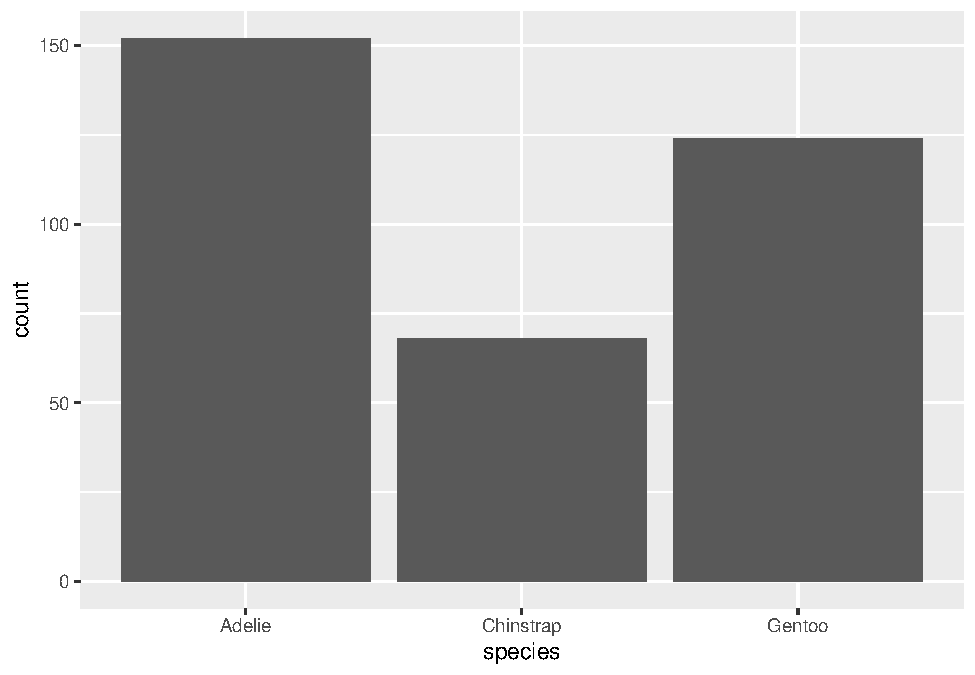
\includegraphics{intro_stats_files/figure-latex/unnamed-chunk-55-1.pdf}

We'll walk through this syntax step by step.

\begin{itemize}
\tightlist
\item
  The first argument of the \texttt{ggplot} command is the name of the tibble, in this case, \texttt{penguins}.
\item
  Next we define the aesthetics using \texttt{aes} and parentheses. Inside the parentheses, we assign any variables we want to plot to aesthetics of the graph. For this analysis, we are only interested in the variable \texttt{species} and for a bar chart, the categorical variable typically goes on the x-axis. That's why it says \texttt{x\ =\ species} inside the \texttt{aes} argument.
\item
  Finally, \texttt{ggplot} needs to know what kind of graph we want. Graph types are called ``geoms'' in the \texttt{ggplot} world, and \texttt{geom\_bar()} tells \texttt{ggplot} to add a ``bar chart layer''. Adding a layer is accomplished by literally typing a plus sign.
\end{itemize}

This can be modified somewhat to give proportions (relative frequencies) on the y-axis instead of counts. Unfortunately, the \texttt{ggplot} syntax is not very transparent here. My recommendation is to copy and paste the code below if you need to make a relative frequency bar chart in the future, making the necessary changes to the tibble and variable names, of course.

\begin{Shaded}
\begin{Highlighting}[]
\FunctionTok{ggplot}\NormalTok{(penguins, }\FunctionTok{aes}\NormalTok{(}\AttributeTok{x =}\NormalTok{ species, }\AttributeTok{y =}\NormalTok{ ..prop.., }\AttributeTok{group =} \DecValTok{1}\NormalTok{)) }\SpecialCharTok{+}
    \FunctionTok{geom\_bar}\NormalTok{()}
\end{Highlighting}
\end{Shaded}

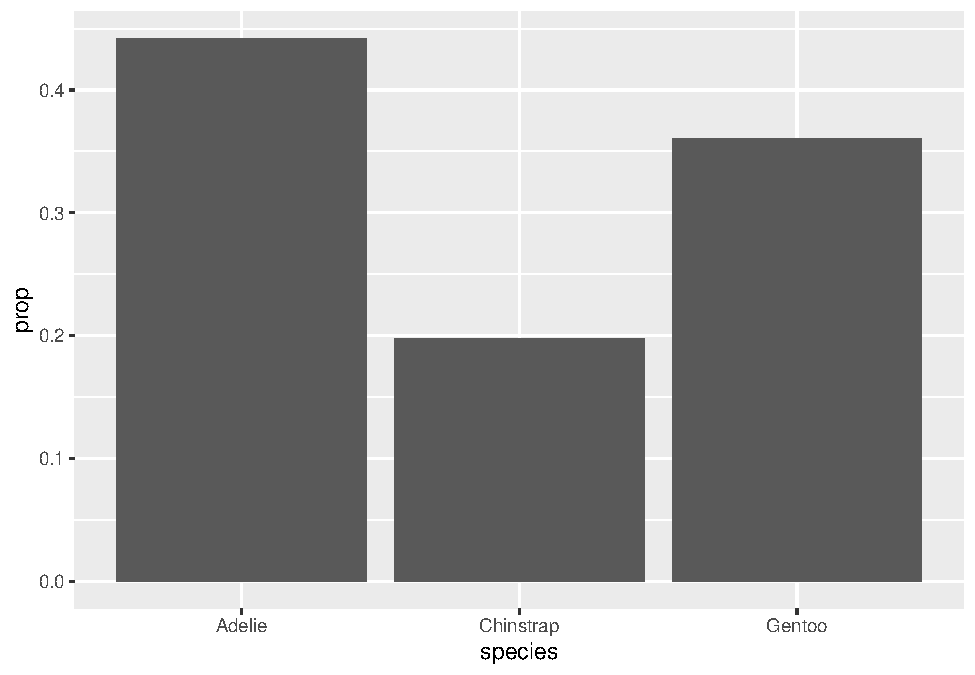
\includegraphics{intro_stats_files/figure-latex/unnamed-chunk-56-1.pdf}

These bar charts are the graphical analogues of a frequency table and a relative frequency table, respectively.

\hypertarget{exercise-4}{%
\paragraph*{Exercise 4}\label{exercise-4}}
\addcontentsline{toc}{paragraph}{Exercise 4}

In a sentence or two at most, describe the distribution of species in this data set.

Please write up your answer here.

\begin{center}\rule{0.5\linewidth}{0.5pt}\end{center}

What about pie charts? Just. Don't.

Seriously. Pie charts suck.\footnote{\url{https://medium.com/the-mission/to-pie-charts-3b1f57bcb34a}}

\hypertarget{categorical-summarizing-two}{%
\section{Summarizing two categorical variables}\label{categorical-summarizing-two}}

A table summarizing two categorical variables is called a \emph{contingency table} (or pivot table, or cross-tabulation, or probably several other terms as well).

For example, we might pose the following question: is the distribution of sex among penguins in our data more or less balanced across the three species?

When we work with two variables, typically we think of one variable as \emph{response} and the other as \emph{predictor}. The response variable is usually the variable of main interest. A predictor variable is another attribute that might predict or explain more about the response variable.

For example, our question is concerned with the sex distribution of penguins. We could create a relative frequency table of sex alone to see if male and female penguins are balanced in the data. In fact, you did that very thing above and saw that, indeed, there were roughly equal numbers of male and female penguins. But is that still true when we divide up the data into the three groups representing the separate species?

Two variables are called \emph{associated} when there is a relationship between them. For example, if sex and species were associated, then the distribution of sex would change depending on the species. Maybe one species of penguin had more females and another had fewer females. Our prediction of the sex distribution would change based on the value of the predictor variable \texttt{species}.

On the other hand, two variables that are not associated are called \emph{independent}. Independent variables are not related. If the sex distribution were the same across all species, then knowledge of the species would not change our predictions about the sex of a penguin. It wouldn't matter because there was no relationship between sex and species.

Most research questions that involve two or more variables are fundamentally questions of whether a response variable is associated with one or more predictor variables, or whether they are independent.

Let's check the contingency table. The \texttt{tabyl} command will place the first variable listed across the rows and the second one listed down the columns. Since we always include column totals, we want the predictor variable to be the column variable so we can see how the predictor groups are distributed in the data. \textbf{Always list the response variable first}.

\begin{Shaded}
\begin{Highlighting}[]
\FunctionTok{tabyl}\NormalTok{(penguins, sex, species) }\SpecialCharTok{\%\textgreater{}\%}
  \FunctionTok{adorn\_totals}\NormalTok{()}
\end{Highlighting}
\end{Shaded}

\begin{verbatim}
##     sex Adelie Chinstrap Gentoo
##  female     73        34     58
##    male     73        34     61
##    <NA>      6         0      5
##   Total    152        68    124
\end{verbatim}

Each column is a group, and our question is whether the distribution of sexes in each column is similar.

The last row of totals is called the \emph{marginal distribution} (because it sits in the ``margin'' of the contingency table). It is equivalent to a frequency table for \texttt{species}.

\hypertarget{exercise-5}{%
\paragraph{Exercise 5}\label{exercise-5}}

Counts can be misleading. For example, there are 73 female Adelie penguins, but only 34 female Chinstrap penguins. Does that mean that Adelie penguins are more likely to be female than Chinstrap penguins? Why or why not?

Please write up your answer here.

\begin{center}\rule{0.5\linewidth}{0.5pt}\end{center}

A more fair way to compare across columns is to create relative frequencies. We can do this with a slightly different \texttt{adorn} command. The following code says that we want to compute column proportions (yes, I know the command is called \texttt{adorn\_percentages}, but these are proportions):

\begin{Shaded}
\begin{Highlighting}[]
\FunctionTok{tabyl}\NormalTok{(penguins, sex, species) }\SpecialCharTok{\%\textgreater{}\%}
    \FunctionTok{adorn\_totals}\NormalTok{() }\SpecialCharTok{\%\textgreater{}\%}
    \FunctionTok{adorn\_percentages}\NormalTok{(}\StringTok{"col"}\NormalTok{)}
\end{Highlighting}
\end{Shaded}

\begin{verbatim}
##     sex     Adelie Chinstrap     Gentoo
##  female 0.48026316       0.5 0.46774194
##    male 0.48026316       0.5 0.49193548
##    <NA> 0.03947368       0.0 0.04032258
##   Total 1.00000000       1.0 1.00000000
\end{verbatim}

If we actually want percentages, we need one more line of code. This command---\texttt{adorn\_pct\_formatting}---is the same as we used before with frequency tables.

\begin{Shaded}
\begin{Highlighting}[]
\FunctionTok{tabyl}\NormalTok{(penguins, sex, species) }\SpecialCharTok{\%\textgreater{}\%}
    \FunctionTok{adorn\_totals}\NormalTok{() }\SpecialCharTok{\%\textgreater{}\%}
    \FunctionTok{adorn\_percentages}\NormalTok{(}\StringTok{"col"}\NormalTok{) }\SpecialCharTok{\%\textgreater{}\%}
    \FunctionTok{adorn\_pct\_formatting}\NormalTok{()}
\end{Highlighting}
\end{Shaded}

\begin{verbatim}
##     sex Adelie Chinstrap Gentoo
##  female  48.0%     50.0%  46.8%
##    male  48.0%     50.0%  49.2%
##    <NA>   3.9%      0.0%   4.0%
##   Total 100.0%    100.0% 100.0%
\end{verbatim}

Now we can see that each column adds up to 100\%. In other words, each species is now on equal footing, and only the distribution of sexes within each group matters.

\hypertarget{exercise-6a}{%
\paragraph{Exercise 6(a)}\label{exercise-6a}}

What percentage of Adelie penguins are male? What percentage of Chinstrap penguins are male? What percentage of Gentoo penguins are male?

Please write up your answer here.

\hypertarget{exercise-6b}{%
\paragraph{Exercise 6(b)}\label{exercise-6b}}

Does sex appear to be associated with species for the penguins in this data set? Or are these variables independent?

Please write up your answer here.

\begin{center}\rule{0.5\linewidth}{0.5pt}\end{center}

The islands of Antarctica on which the penguins were observed and measured are recorded in the variable called \texttt{island}. Is the distribution of the three species of penguin the same (or similar) on the three islands?

\hypertarget{exercise-7a}{%
\paragraph{Exercise 7(a)}\label{exercise-7a}}

Choosing which variables play the roles of response and predictor can be tricky. For the question above, with \texttt{species} and \texttt{island}, which is response and which is predictor?

One way to think about this is to ask the following two questions and see which one is closer to the question asked:

\begin{itemize}
\tightlist
\item
  Given information about the species, are you interested in which island the penguin lives on? If so, \texttt{species} is a predictor and \texttt{island} is response. (You are using \texttt{species} to predict \texttt{island}.)
\item
  Given information about the island, are you interested in the species of the penguin? If so, \texttt{island} is a predictor and \texttt{species} is response. (You are using \texttt{island} to predict \texttt{species}.)
\end{itemize}

Please write up your answer here.

\hypertarget{exercise-7b}{%
\paragraph{Exercise 7(b)}\label{exercise-7b}}

Create a contingency table with percentages. List \texttt{species} first, followed by \texttt{island}. (Hey, that's hint in case you need to go back and change your answer to part (a).)

\begin{Shaded}
\begin{Highlighting}[]
\CommentTok{\# Add code here to create a contingency table with percentages.}
\end{Highlighting}
\end{Shaded}

\hypertarget{exercise-7c}{%
\paragraph{Exercise 7(c)}\label{exercise-7c}}

Finally, comment on the association or independence of the two variables.

Please write up your answer here.

\hypertarget{categorical-graphing-two}{%
\section{Graphing two categorical variables}\label{categorical-graphing-two}}

A somewhat effective way to display two categorical variables is with a side-by-side bar chart. Here is the \texttt{ggplot} code for the relationship between \texttt{sex} and \texttt{species}.

\begin{Shaded}
\begin{Highlighting}[]
\FunctionTok{ggplot}\NormalTok{(penguins, }\FunctionTok{aes}\NormalTok{(}\AttributeTok{fill =}\NormalTok{ sex, }\AttributeTok{x =}\NormalTok{ species)) }\SpecialCharTok{+}
    \FunctionTok{geom\_bar}\NormalTok{(}\AttributeTok{position =} \StringTok{"dodge"}\NormalTok{)}
\end{Highlighting}
\end{Shaded}

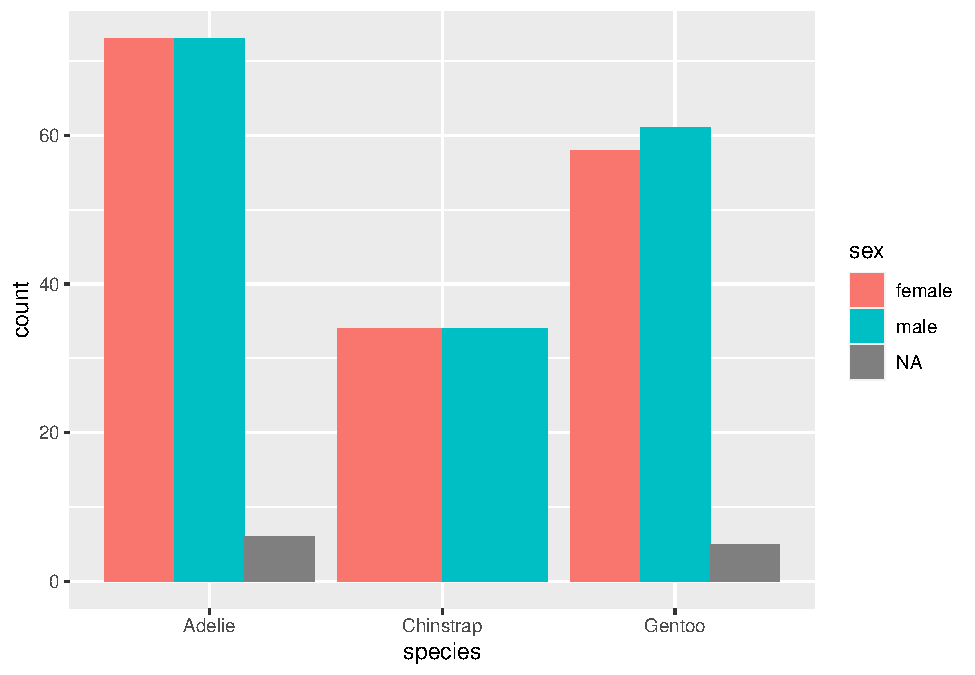
\includegraphics{intro_stats_files/figure-latex/unnamed-chunk-61-1.pdf}

This is somewhat different from the first \texttt{ggplot} example you saw above, so let's take a moment to go through it.

\begin{itemize}
\tightlist
\item
  The first argument is the data frame \texttt{penguins}; no mystery there.
\item
  The second aesthetic \texttt{x\ =\ species} also makes a lot of sense. As \texttt{species} is our predictor variable---we're using species to group the penguins, and then within each species, we're interested in the sex distribution---\texttt{species} goes on the x-axis.
\item
  However, \texttt{sex} does not go on the y-axis! (This is a very common mistake for novices.) The y-axis of a bar chart is always a count or a proportion/percentage, so no variable should ever go on the y-axis of a bar chart. In that case, how does \texttt{sex} enter the picture? Through the use of color! The aesthetic \texttt{fill\ =\ sex} says to use the \texttt{sex} variable to shade or ``fill'' the bars with different colors. You'll also notice that \texttt{ggplot} makes a legend automatically with the colors so you can see which color corresponds to which value (in this case, ``female'', ``male'', or ``NA'' for the missing data).
\end{itemize}

Another unusual feature is the argument \texttt{position\ =\ "dodge"} in the \texttt{geom\_bar} layer. Let's see what happens if we remove it.

\begin{Shaded}
\begin{Highlighting}[]
\FunctionTok{ggplot}\NormalTok{(penguins, }\FunctionTok{aes}\NormalTok{(}\AttributeTok{fill =}\NormalTok{ sex, }\AttributeTok{x =}\NormalTok{ species)) }\SpecialCharTok{+} 
    \FunctionTok{geom\_bar}\NormalTok{()}
\end{Highlighting}
\end{Shaded}

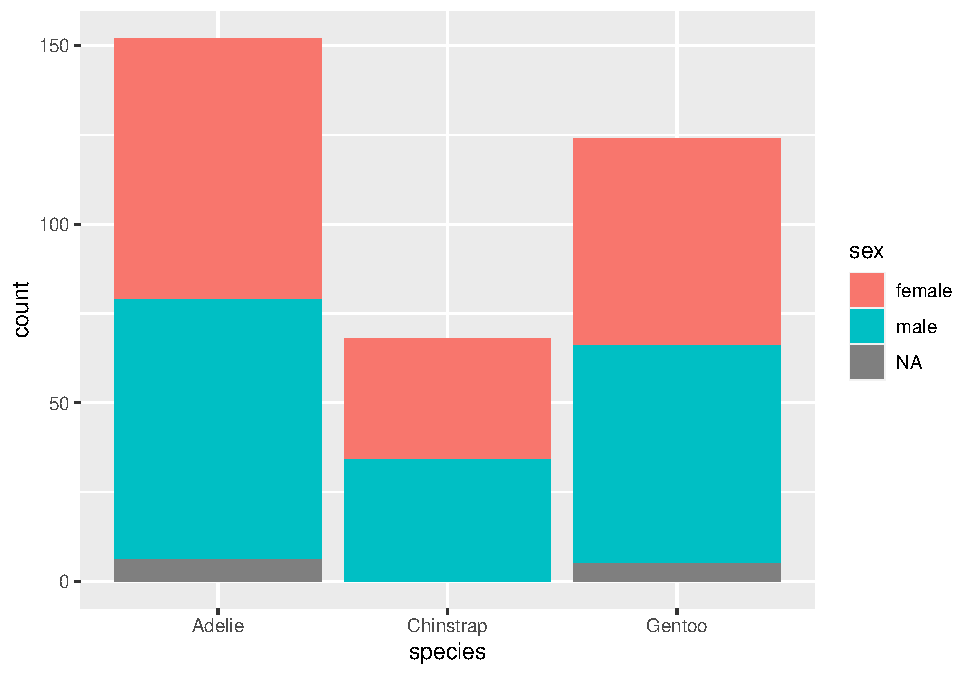
\includegraphics{intro_stats_files/figure-latex/unnamed-chunk-62-1.pdf}

We get a stacked bar chart! This is another popular way of displaying two categorical variables, but we don't tend to prefer it. Notice how difficult it is to compare the number of females across species; since there is no common baseline for the red segments of each bar, it is harder to determine which ones are bigger or smaller. (In this case, it's fairly clear, but there are plenty of data sets for which the counts might be a lot closer.)

So let's agree to use side-by-side bar charts. There is still one aspect of the side-by-side bar chart that is misleading, though. For example, the red bar for Adelie penguins is bigger than the red bar for Gentoo penguins. Does this mean Adelie penguins are more likely to be female?

This is the same issue we identified in an exercise above. To fix this problem, a better option here would be to use relative frequencies (i.e., proportions/percentages within each group) instead of counts on the y-axis. This is analogous to using proportions/percentages in a contingency table. Unfortunately, it is rather difficult to do this with \texttt{ggplot}. A compromise is available: by using \texttt{position\ =\ fill}, you can create a stacked bar chart that scales every group to 100\%. Making comparisons across groups can still be hard, as explained above for any kind of stacked bar chart, but it works okay if there are only two categories in the response variable (as is almost the case with \texttt{sex} here, although the missing data distorts things a little at the bottom).

\begin{Shaded}
\begin{Highlighting}[]
\FunctionTok{ggplot}\NormalTok{(penguins, }\FunctionTok{aes}\NormalTok{(}\AttributeTok{fill =}\NormalTok{ sex, }\AttributeTok{x =}\NormalTok{ species)) }\SpecialCharTok{+}
    \FunctionTok{geom\_bar}\NormalTok{(}\AttributeTok{position =} \StringTok{"fill"}\NormalTok{)}
\end{Highlighting}
\end{Shaded}

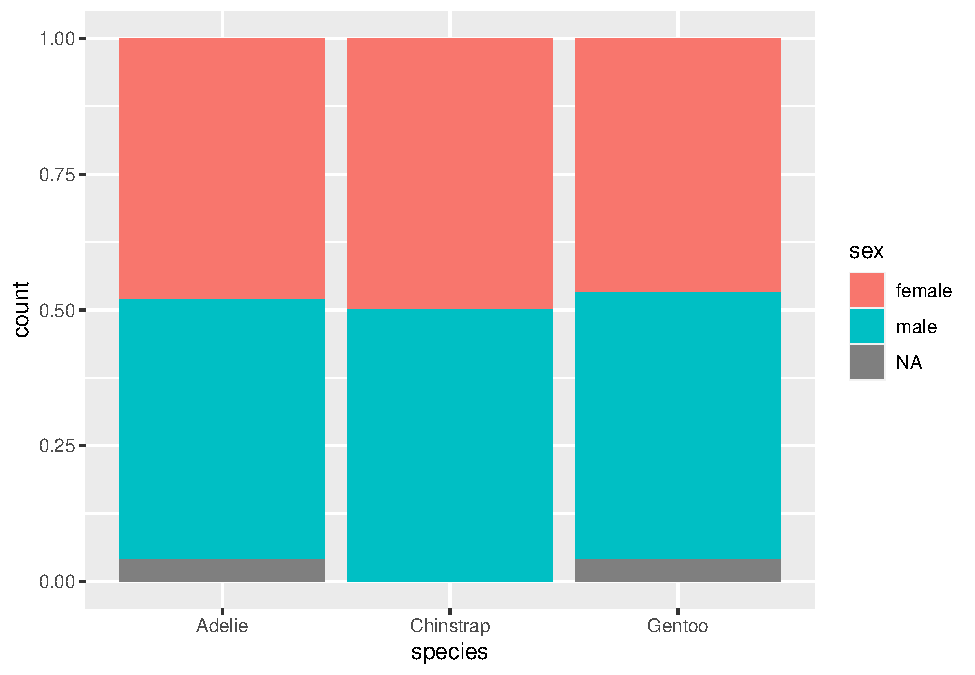
\includegraphics{intro_stats_files/figure-latex/unnamed-chunk-63-1.pdf}

This graph does correctly show that the sexes are pretty much equally balances across all three species.

\hypertarget{exercise-8a}{%
\paragraph*{Exercise 8(a)}\label{exercise-8a}}
\addcontentsline{toc}{paragraph}{Exercise 8(a)}

Using \texttt{species} and \texttt{island}, create a side-by-side bar chart. Be careful, though, to change the sample code above to make sure \texttt{species} is now the response variable (using the \texttt{fill} aesthetic) and that \texttt{island} is the explanatory variable (using \texttt{x}). (Hey, that's another hint to go back and look at the previous exercise and make sure you got part (a) right!)

\begin{Shaded}
\begin{Highlighting}[]
\CommentTok{\# Add code here to make a side{-}by{-}side bar chart.}
\end{Highlighting}
\end{Shaded}

\hypertarget{exercise-8b}{%
\paragraph*{Exercise 8(b)}\label{exercise-8b}}
\addcontentsline{toc}{paragraph}{Exercise 8(b)}

Comment on the association or independence of the two variables.

Please write up your answer here.

\hypertarget{categorical-recoding}{%
\section{Recoding factor variables}\label{categorical-recoding}}

As mentioned earlier, there are situations where a categorical variable is not recorded in R as a factor variable. Let's look at the \texttt{year} variable:

\begin{Shaded}
\begin{Highlighting}[]
\FunctionTok{glimpse}\NormalTok{(penguins}\SpecialCharTok{$}\NormalTok{year)}
\end{Highlighting}
\end{Shaded}

\begin{verbatim}
##  int [1:344] 2007 2007 2007 2007 2007 2007 2007 2007 2007 2007 ...
\end{verbatim}

These appear as integers. Yes, years are whole numbers, but why might this variable be treated as categorical data and not numerical data?

\hypertarget{exercise-9a}{%
\paragraph*{Exercise 9(a)}\label{exercise-9a}}
\addcontentsline{toc}{paragraph}{Exercise 9(a)}

Use the \texttt{tabyl} command to create a frequency table for \texttt{year}.

\begin{Shaded}
\begin{Highlighting}[]
\CommentTok{\# Add code here to make a frequency table for year.}
\end{Highlighting}
\end{Shaded}

\hypertarget{exercise-9b}{%
\paragraph*{Exercise 9(b)}\label{exercise-9b}}
\addcontentsline{toc}{paragraph}{Exercise 9(b)}

Why is \texttt{year} better thought of as categorical data and not numerical data (at least for this data set---we're not claiming years should always be treated as categorical)?

Please write up your answer here.

\begin{center}\rule{0.5\linewidth}{0.5pt}\end{center}

While the \texttt{tabyl} command seemed to work just fine with the \texttt{year} data in integer format, there are other commands that will not work so well. For example, \texttt{ggplot} often fails to do the right thing when a categorical variable is coded as a number. Therefore, we need a way to change numerically coded variables to factors.

The code below uses a command called \texttt{mutate} that takes an old variable and creates a new variable. (You'll learn more about this command in a later chapter. For now, you can just copy and paste this code if you need it again.) The name of the new variable can be anything we want; we'll just call it \texttt{year\_fct}. Then the real work is being done by the \texttt{as\_factor} command that concerts the numeric \texttt{year} variable into a factor variable.

Observe the effect below:

\begin{Shaded}
\begin{Highlighting}[]
\NormalTok{penguins }\OtherTok{\textless{}{-}}\NormalTok{ penguins }\SpecialCharTok{\%\textgreater{}\%}
    \FunctionTok{mutate}\NormalTok{(}\AttributeTok{year\_fct =} \FunctionTok{as\_factor}\NormalTok{(year))}
\FunctionTok{glimpse}\NormalTok{(penguins)}
\end{Highlighting}
\end{Shaded}

\begin{verbatim}
## Rows: 344
## Columns: 9
## $ species           <fct> Adelie, Adelie, Adelie, Adelie, Adelie, Adelie, Adel~
## $ island            <fct> Torgersen, Torgersen, Torgersen, Torgersen, Torgerse~
## $ bill_length_mm    <dbl> 39.1, 39.5, 40.3, NA, 36.7, 39.3, 38.9, 39.2, 34.1, ~
## $ bill_depth_mm     <dbl> 18.7, 17.4, 18.0, NA, 19.3, 20.6, 17.8, 19.6, 18.1, ~
## $ flipper_length_mm <int> 181, 186, 195, NA, 193, 190, 181, 195, 193, 190, 186~
## $ body_mass_g       <int> 3750, 3800, 3250, NA, 3450, 3650, 3625, 4675, 3475, ~
## $ sex               <fct> male, female, female, NA, female, male, female, male~
## $ year              <int> 2007, 2007, 2007, 2007, 2007, 2007, 2007, 2007, 2007~
## $ year_fct          <fct> 2007, 2007, 2007, 2007, 2007, 2007, 2007, 2007, 2007~
\end{verbatim}

\hypertarget{exercise-10a}{%
\paragraph*{Exercise 10(a)}\label{exercise-10a}}
\addcontentsline{toc}{paragraph}{Exercise 10(a)}

Make a contingency table of the species measured in each year using counts. Use the \texttt{species} variable first, followed by the new factor variable \texttt{year\_fct}. (Think about why that order makes sense. \textbf{We will always list the response variable first so that the categories of interest will be the rows and the groups will be the columns.})

\begin{Shaded}
\begin{Highlighting}[]
\CommentTok{\# Add code here to make a contingency table for species and year with counts.}
\end{Highlighting}
\end{Shaded}

\hypertarget{exercise-10b}{%
\paragraph*{Exercise 10(b)}\label{exercise-10b}}
\addcontentsline{toc}{paragraph}{Exercise 10(b)}

Make a contingency table of the species measured in each year using column percentages (\emph{not} proportions). (Again, be sure to use the new factor variable \texttt{year\_fct}, not the old variable \texttt{year}.)

\begin{Shaded}
\begin{Highlighting}[]
\CommentTok{\# Add code here to make a contingency table for species and year with percentages.}
\end{Highlighting}
\end{Shaded}

\hypertarget{exercise-10c}{%
\paragraph*{Exercise 10(c)}\label{exercise-10c}}
\addcontentsline{toc}{paragraph}{Exercise 10(c)}

How similar or dissimilar are the distributions of species across the three years of the study?

Please write up your answer here.

\hypertarget{categorical-pub}{%
\section{Publication-ready graphics}\label{categorical-pub}}

Let's go back to the first relative frequency bar chart from this chapter.

\begin{Shaded}
\begin{Highlighting}[]
\FunctionTok{ggplot}\NormalTok{(penguins, }\FunctionTok{aes}\NormalTok{(}\AttributeTok{x =}\NormalTok{ species, }\AttributeTok{y =}\NormalTok{ ..prop.., }\AttributeTok{group =} \DecValTok{1}\NormalTok{)) }\SpecialCharTok{+}
    \FunctionTok{geom\_bar}\NormalTok{()}
\end{Highlighting}
\end{Shaded}

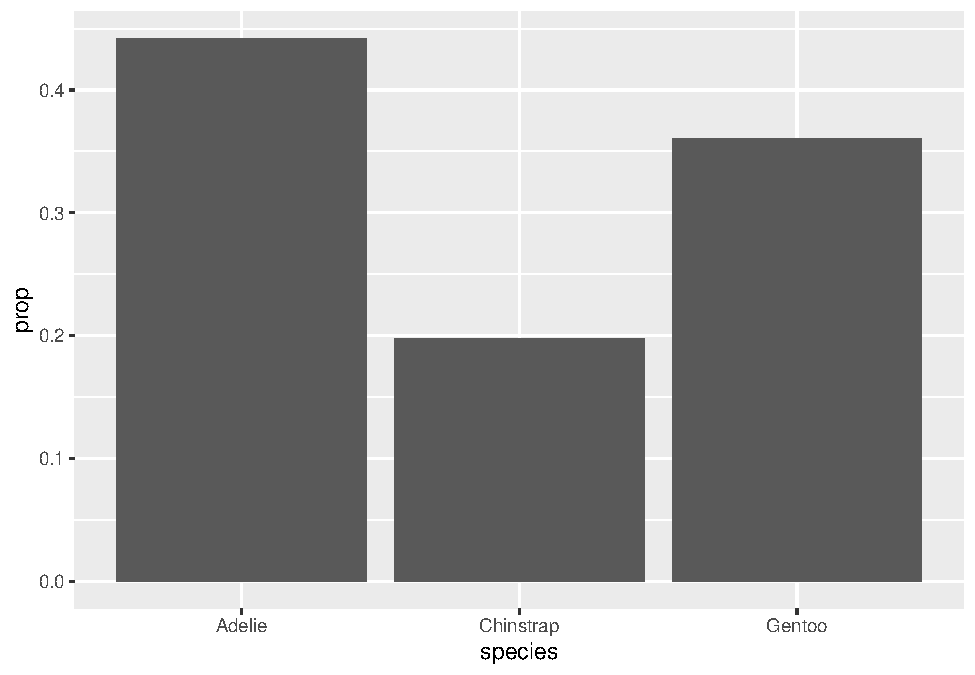
\includegraphics{intro_stats_files/figure-latex/unnamed-chunk-70-1.pdf}

The variable name \texttt{species} is already informative, but the y-axis is labeled with ``prop''. Also note that this graph could use a title. We can do all this with \texttt{labs} (for labels). Observe:

\begin{Shaded}
\begin{Highlighting}[]
\FunctionTok{ggplot}\NormalTok{(penguins, }\FunctionTok{aes}\NormalTok{(}\AttributeTok{x =}\NormalTok{ species, }\AttributeTok{y =}\NormalTok{ ..prop.., }\AttributeTok{group =} \DecValTok{1}\NormalTok{)) }\SpecialCharTok{+}
    \FunctionTok{geom\_bar}\NormalTok{() }\SpecialCharTok{+}
    \FunctionTok{labs}\NormalTok{(}\AttributeTok{title =} \StringTok{"Distribution of species"}\NormalTok{,}
         \AttributeTok{y =} \StringTok{"Proportion"}\NormalTok{,}
         \AttributeTok{x =} \StringTok{"Species"}\NormalTok{)}
\end{Highlighting}
\end{Shaded}

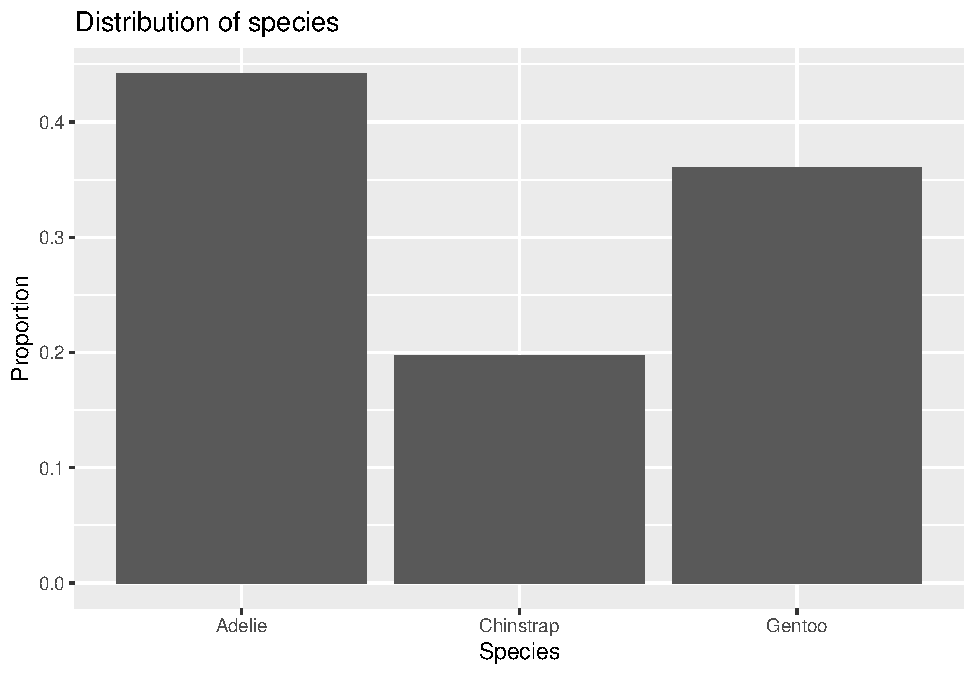
\includegraphics{intro_stats_files/figure-latex/unnamed-chunk-71-1.pdf}

\hypertarget{exercise-11}{%
\paragraph*{Exercise 11}\label{exercise-11}}
\addcontentsline{toc}{paragraph}{Exercise 11}

Modify the following side-by-side bar chart by adding a title and labels for both the fill variable and the x-axis variable. (Hint: you can use \texttt{fill\ =\ sex} inside the \texttt{labs} command just like you used \texttt{title}, \texttt{y}, and \texttt{x}.)

\begin{Shaded}
\begin{Highlighting}[]
\CommentTok{\# Modify the following side{-}by{-}side bar chart by adding a title and }
\CommentTok{\# labels for both the x{-}axis and the fill variable.}
\FunctionTok{ggplot}\NormalTok{(penguins, }\FunctionTok{aes}\NormalTok{(}\AttributeTok{fill =}\NormalTok{ sex, }\AttributeTok{x =}\NormalTok{ species)) }\SpecialCharTok{+}
    \FunctionTok{geom\_bar}\NormalTok{(}\AttributeTok{position =} \StringTok{"dodge"}\NormalTok{)}
\end{Highlighting}
\end{Shaded}

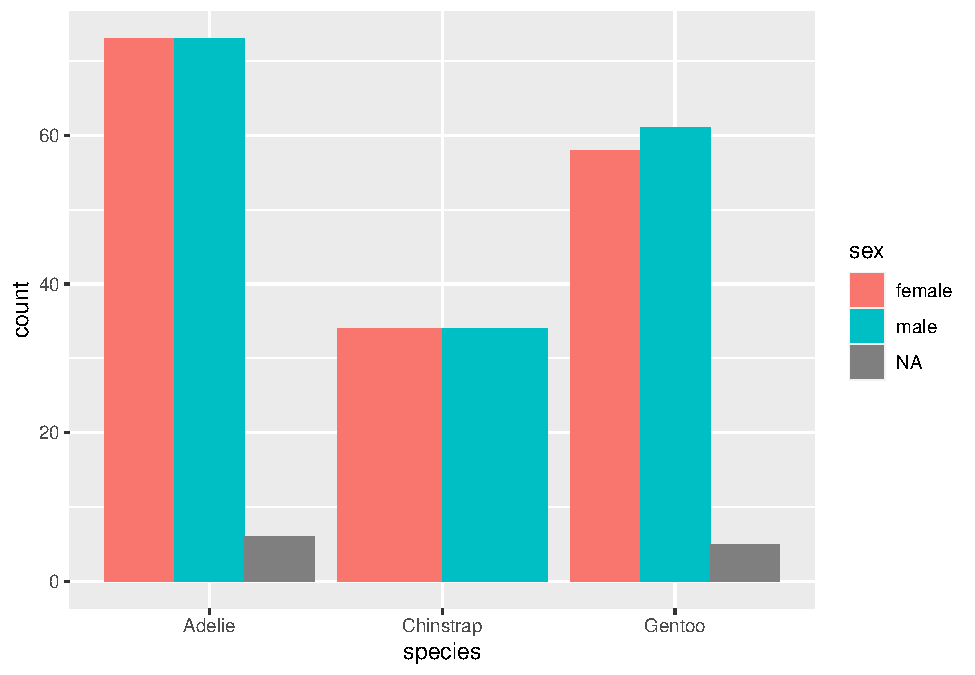
\includegraphics{intro_stats_files/figure-latex/unnamed-chunk-72-1.pdf}

\hypertarget{categorical-summary}{%
\section{Plotting summary data}\label{categorical-summary}}

Everything we did above was summarizing \emph{raw data}; that is, the data consisted of all the observations for each individual penguin. Often, though, when you find data out in the wild, that data will be summarized into a table already and you may not have access to the raw data.

For example, let's suppose that you found some data online, but it looked like this:

\begin{longtable}[]{@{}ll@{}}
\toprule()
species & count \\
\midrule()
\endhead
Adelie & 152 \\
Chinstrap & 68 \\
Gentoo & 124 \\
\bottomrule()
\end{longtable}

This raises two questions:

\begin{enumerate}
\def\labelenumi{\arabic{enumi}.}
\tightlist
\item
  How would you get this data into R?
\item
  How would you plot the data?
\end{enumerate}

To answer the first question, we show you how to create your own tibble. Here is the syntax:

\begin{Shaded}
\begin{Highlighting}[]
\NormalTok{penguin\_species\_table }\OtherTok{\textless{}{-}} \FunctionTok{tibble}\NormalTok{(}
    \AttributeTok{species =} \FunctionTok{c}\NormalTok{(}\StringTok{"Adelie"}\NormalTok{, }\StringTok{"Chinstrap"}\NormalTok{, }\StringTok{"Gentoo"}\NormalTok{),}
    \AttributeTok{count =} \FunctionTok{c}\NormalTok{(}\DecValTok{152}\NormalTok{, }\DecValTok{68}\NormalTok{, }\DecValTok{124}\NormalTok{)}
\NormalTok{)}
\NormalTok{penguin\_species\_table}
\end{Highlighting}
\end{Shaded}

\begin{verbatim}
## # A tibble: 3 x 2
##   species   count
##   <chr>     <dbl>
## 1 Adelie      152
## 2 Chinstrap    68
## 3 Gentoo      124
\end{verbatim}

Basically, the \texttt{tibble} command creates a new tibble. Then each column of data must be entered manually as a ``vector'' using the \texttt{c} to group all the data values together for each column. Be careful about the placement of quotation marks, commas, and parentheses.

Once we have our summary data, we want to make a bar chart. But this won't work:

\begin{Shaded}
\begin{Highlighting}[]
\FunctionTok{ggplot}\NormalTok{(penguin\_species\_table, }\FunctionTok{aes}\NormalTok{(}\AttributeTok{x =}\NormalTok{ species)) }\SpecialCharTok{+}
    \FunctionTok{geom\_bar}\NormalTok{()}
\end{Highlighting}
\end{Shaded}

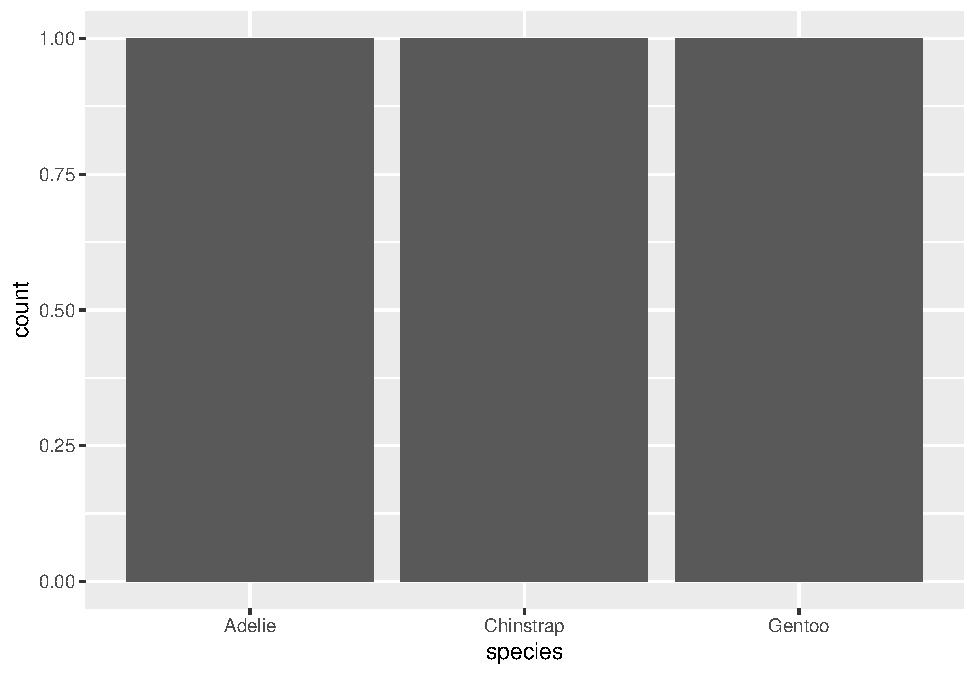
\includegraphics{intro_stats_files/figure-latex/unnamed-chunk-74-1.pdf}

\hypertarget{exercise-12}{%
\paragraph*{Exercise 12}\label{exercise-12}}
\addcontentsline{toc}{paragraph}{Exercise 12}

Explain what went wrong with the previous command? Why does \texttt{ggplot} think that each species has count 1?

Please write up your answer here.

\begin{center}\rule{0.5\linewidth}{0.5pt}\end{center}

Instead, we need to use \texttt{geom\_col}. This works a lot like \texttt{geom\_bar} except that it also requires a \texttt{y} value in its aesthetics to force the command to look for the counts in some other variable in the data.

\begin{Shaded}
\begin{Highlighting}[]
\FunctionTok{ggplot}\NormalTok{(penguin\_species\_table, }\FunctionTok{aes}\NormalTok{(}\AttributeTok{x =}\NormalTok{ species, }\AttributeTok{y =}\NormalTok{ count)) }\SpecialCharTok{+}
    \FunctionTok{geom\_col}\NormalTok{()}
\end{Highlighting}
\end{Shaded}

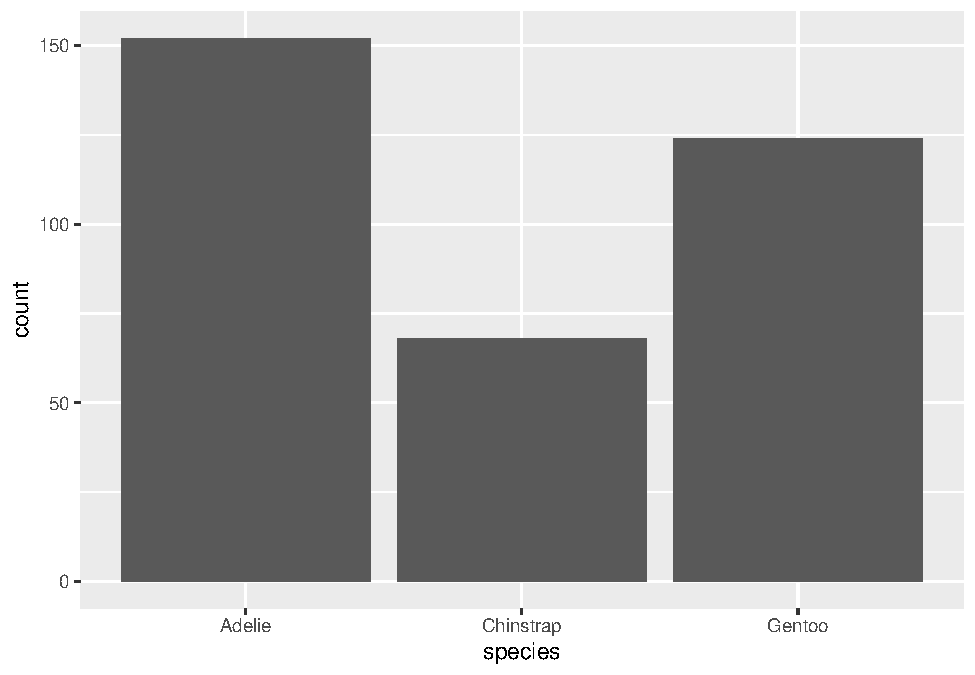
\includegraphics{intro_stats_files/figure-latex/unnamed-chunk-75-1.pdf}

\hypertarget{exercise-13a}{%
\paragraph*{Exercise 13(a)}\label{exercise-13a}}
\addcontentsline{toc}{paragraph}{Exercise 13(a)}

Use the \texttt{tabyl} command to create a frequency table for \texttt{island}.

\begin{Shaded}
\begin{Highlighting}[]
\CommentTok{\# Add code here to create a frequency table for island}
\end{Highlighting}
\end{Shaded}

\hypertarget{exercise-13b}{%
\paragraph*{Exercise 13(b)}\label{exercise-13b}}
\addcontentsline{toc}{paragraph}{Exercise 13(b)}

Use the \texttt{tibble} command to create a new tibble manually that contains the frequency data for the \texttt{island} variable. It should have two columns, one called \texttt{island} and the other called \texttt{count}. Name it \texttt{penguin\_island\_table}.

\begin{Shaded}
\begin{Highlighting}[]
\CommentTok{\# Add code here to create a tibble with frequency data for island}
\end{Highlighting}
\end{Shaded}

\hypertarget{exercise-13c}{%
\paragraph*{Exercise 13(c)}\label{exercise-13c}}
\addcontentsline{toc}{paragraph}{Exercise 13(c)}

Use \texttt{ggplot} with \texttt{geom\_col} to create a bar chart for island.

\begin{Shaded}
\begin{Highlighting}[]
\CommentTok{\# Add code here to create a bar chart for island}
\end{Highlighting}
\end{Shaded}

\hypertarget{categorical-conclusion}{%
\section{Conclusion}\label{categorical-conclusion}}

You can summarize a single categorical variable using a frequency table. For only one categorical variable, a graph is usually overkill, but if you really want a graph, the bar chart is the best option. Both raw counts and proportions/percentages can be useful.

We use contingency tables to summarize two categorical variables. Unless groups are of equal size, raw counts can be incredibly misleading here. You should include proportions/percentages to be able to compare the distributions across groups. If the proportions/percentages are roughly the same, the variables are more likely to be independent, whereas if the proportions/percentages are different, there may be an association between the variables. For graphing, the best choice is usually a side-by-side bar chart. A stacked bar chart will also work, especially if using relative frequencies on the y-axis, but it can be hard to compare across groups when the response variable has three or more categories.

Sometimes we come across categorical data that is recorded using numbers. Many R commands will not work properly if they expect factors and receive numbers, so we use the \texttt{mutate} command to create a new variable along with \texttt{as\_factor} to convert the numbers to categories.

Sometimes we come across summary data instead of raw data. We can then manually create tibbles with that summary data and use \texttt{geom\_col} instead of \texttt{geom\_bar} to graph it.

\hypertarget{categorical-prep}{%
\subsection{Preparing and submitting your assignment}\label{categorical-prep}}

\begin{enumerate}
\def\labelenumi{\arabic{enumi}.}
\tightlist
\item
  From the ``Run'' menu, select ``Restart R and Run All Chunks''.
\item
  Deal with any code errors that crop up. Repeat steps 1---2 until there are no more code errors.
\item
  Spell check your document by clicking the icon with ``ABC'' and a check mark.
\item
  Hit the ``Preview'' button one last time to generate the final draft of the \texttt{.nb.html} file.
\item
  Proofread the HTML file carefully. If there are errors, go back and fix them, then repeat steps 1--5 again.
\end{enumerate}

If you have completed this chapter as part of a statistics course, follow the directions you receive from your professor to submit your assignment.

\hypertarget{numerical}{%
\chapter{Numerical data}\label{numerical}}

2.0

\hypertarget{functions-introduced-in-this-chapter-3}{%
\subsection*{Functions introduced in this chapter}\label{functions-introduced-in-this-chapter-3}}
\addcontentsline{toc}{subsection}{Functions introduced in this chapter}

\texttt{mean}, \texttt{sd}, \texttt{var}, \texttt{median}, \texttt{sort}, \texttt{IQR}, \texttt{quantile}, \texttt{summary}, \texttt{min}, \texttt{max}, \texttt{geom\_histogram}, \texttt{geom\_point}, \texttt{geom\_boxplot}, \texttt{facet\_grid}

\hypertarget{numerical-intro}{%
\section{Introduction}\label{numerical-intro}}

In this chapter, we'll learn about numerical data and how to summarize it through summary statistics and graphs.

\hypertarget{numerical-install}{%
\subsection{Install new packages}\label{numerical-install}}

There are no new packages used in this chapter.

\hypertarget{numerical-download}{%
\subsection{Download the R notebook file}\label{numerical-download}}

Check the upper-right corner in RStudio to make sure you're in your \texttt{intro\_stats} project. Then click on the following link to download this chapter as an R notebook file (\texttt{.Rmd}).

https://vectorposse.github.io/intro\_stats/chapter\_downloads/04-numerical\_data.Rmd

Once the file is downloaded, move it to your project folder in RStudio and open it there.

\hypertarget{numerical-restart}{%
\subsection{Restart R and run all chunks}\label{numerical-restart}}

In RStudio, select ``Restart R and Run All Chunks'' from the ``Run'' menu.

\hypertarget{numerical-load}{%
\subsection{Load packages}\label{numerical-load}}

We load the \texttt{tidyverse} package to get \texttt{ggplot2} and the \texttt{palmerpenguins} package to work with the penguin data.

\begin{Shaded}
\begin{Highlighting}[]
\FunctionTok{library}\NormalTok{(tidyverse)}
\FunctionTok{library}\NormalTok{(palmerpenguins)}
\end{Highlighting}
\end{Shaded}

\hypertarget{numerical-notation}{%
\section{A note about mathematical notation}\label{numerical-notation}}

From time to time, we will use mathematical notation that can't be typed directly on the keyboard. For example, let's suppose we want to typeset the quadratic formula, which involves a complicated fraction as well as a square root symbol.

When such notation appears, it will be surrounded by double dollar signs as follows:

\[
x = \frac{-b \pm \sqrt{b^{2} - 4ac}}{2a}
\]

The R Notebook will interpret this special mathematical notation and render it on the screen as well as in the HTML document.\footnote{This notation is part of a mathematical document preparation system called LaTeX, pronounced ``Lay-tek'' (not like the rubbery substance).} If the nicely formatted formula does not appear on your screen, place your cursor anywhere inside the math formula and hit Ctrl-Enter or Cmd-Enter (PC or Mac respectively).

Sometimes, we want such math to appear inline. We can do this with single dollar signs. For example, the distance formula is \(d = \sqrt{(x_{2} - x_{1})^{2} + (y_{2} - y_{1})^{2}}\), a fact you may have learned a long time ago.

This will \emph{not} render visually in the R Notebook, but it will show up in the HTML file. If you want to check that it worked properly without having to preview the HTML, you can either hover your cursor over the math formula and wait a second, or you can place your cursor anywhere inside the math formula and hit Ctrl-Enter or Cmd-Enter (PC or Mac respectively) to see a pop-up window previewing the mathematical content properly formatted.

You will be shown examples of any mathematical notation you need to use in any given chapter, so feel free to copy/paste/modify any math notation you need.

\hypertarget{numerical-statistics}{%
\section{Statistics}\label{numerical-statistics}}

The word ``statistics'' has several meanings. On one hand, it's an entire field of study, as in the subject of this course. More specifically, though, a ``statistic'' is any kind of numerical summary of data. While there are many ways to summarize data, they mostly fall into two main flavors: measures of \emph{center} and measures of \emph{spread}. Measures of center try to estimate some kind of average, middle, or common value in data. Measures of spread try to estimate something like the width, range, variability, or uncertainty of data.

There are two pairs of measurements that we will learn about in this chapter: the mean/standard deviation, and the median/IQR.

\hypertarget{numerical-mean-sd}{%
\subsection{Mean and standard deviation}\label{numerical-mean-sd}}

The first pair of the summary statistics we'll discuss consists of the mean and the standard deviation.

The \emph{mean} of a variable \(y\)---denoted \(\bar{y}\) and pronounced ``y bar''---is calculated by summing all the values of the variable, and dividing by the total number of observations. In formula form, this is

\[
\bar{y} = \frac{\sum y}{n}.
\]

This is a measure of center since it estimates the ``middle'' of a set of numbers. It is calculated in R using the \texttt{mean} command.

Throughout this chapter, we will be using the \texttt{penguins} data set. (If you need a reminder, look at the help file for \texttt{penguins} using one of the methods discussed in Chapter 2.)

If we want to calculate the mean body mass of our penguins (in grams), we type the following:

\begin{Shaded}
\begin{Highlighting}[]
\FunctionTok{mean}\NormalTok{(penguins}\SpecialCharTok{$}\NormalTok{body\_mass\_g)}
\end{Highlighting}
\end{Shaded}

\begin{verbatim}
## [1] NA
\end{verbatim}

Unfortunately, this didn't give us an answer. As you may recall from previous chapters, this is because we are missing several values of body mass in this data. We need an extra piece of code to tell R to ignore that missing data and give us the mean of the valid data.

\begin{Shaded}
\begin{Highlighting}[]
\FunctionTok{mean}\NormalTok{(penguins}\SpecialCharTok{$}\NormalTok{body\_mass\_g, }\AttributeTok{na.rm =} \ConstantTok{TRUE}\NormalTok{)}
\end{Highlighting}
\end{Shaded}

\begin{verbatim}
## [1] 4201.754
\end{verbatim}

(The term \texttt{na.rm} stands for ``NA remove''.)

We never leave such numbers without interpretation. In a full, contextually meaningful sentence, we might say, ``The mean body mass of this group of penguins is approximately 4200 grams.''

Notice that we mentioned the penguins, placing this number in context, and we mentioned the units of measurement, grams. (Otherwise, what would this number mean? 4200 pounds? Okay, probably not, but you should always mention the units of measurement.) Also notice that we rounded the final value. A gram is a very small unit of measurement, so there is no need to report this value to many decimal places.

If we use inline code, we can say, ``The mean body mass of this group of penguins is 4201.754386 grams.'' There are ways of rounding this number as well, but it's a bit of a hassle to do so in inline code.

The corresponding measure of spread is the \emph{standard deviation}. Usually this is called \(s\) and is calculated using a much more complicated formula:

\[
s = \sqrt{\frac{\sum (y - \bar{y})^2}{n - 1}}.
\]

This is a measure of spread because the \((y - \bar{y})\) term measures the how far away each data point is from the mean.

In R, this is calculated with the \texttt{sd} command. Again, we'll need to add \texttt{na.rm\ =\ TRUE}.

\begin{Shaded}
\begin{Highlighting}[]
\FunctionTok{sd}\NormalTok{(penguins}\SpecialCharTok{$}\NormalTok{body\_mass\_g, }\AttributeTok{na.rm =} \ConstantTok{TRUE}\NormalTok{)}
\end{Highlighting}
\end{Shaded}

\begin{verbatim}
## [1] 801.9545
\end{verbatim}

``The standard deviation of this group of penguins is about 801 grams.''

Or using inline code:

``The standard deviation of this group of penguins is 801.9545357 grams.''

The mean and the standard deviation should always be reported together. One without the other is incomplete and potentially misleading.

Another related measurement is the \emph{variance}, but this is nothing more than the standard deviation squared:

\[
s^2 = \frac{\sum (y - \bar{y})^2}{n - 1}.
\]

(Compare this formula to the one for the standard deviation. Nothing has changed except for the removal of the square root.) We rarely use the variance in an introductory stats class because it's not as interpretable as the standard deviation. The main reason for this is units. If the data units are grams, then both the mean and the standard deviation are also reported in grams. The variance has units of ``grams squared'', but what does that even mean? If you need to calculate the variance in R, the command is \texttt{var}.

\begin{Shaded}
\begin{Highlighting}[]
\FunctionTok{var}\NormalTok{(penguins}\SpecialCharTok{$}\NormalTok{body\_mass\_g, }\AttributeTok{na.rm =} \ConstantTok{TRUE}\NormalTok{)}
\end{Highlighting}
\end{Shaded}

\begin{verbatim}
## [1] 643131.1
\end{verbatim}

You can check and see that the number above really is just 801.9545357 squared. Regarding the inline code in the previous sentence, remember, in the R Notebook, you can click inside the inline code and hit Ctrl-Enter or Cmd-Enter. In the HTML document, the number will be calculated and will magically appear.

\hypertarget{numerical-median-iqr}{%
\subsection{Median and IQR}\label{numerical-median-iqr}}

Another choice for measuring the center and spread of a data set is the median and the IQR.

The median is just the middle value if the list of values is ordered. In R, it is calculated using the \texttt{median} command.

\begin{Shaded}
\begin{Highlighting}[]
\FunctionTok{median}\NormalTok{(penguins}\SpecialCharTok{$}\NormalTok{body\_mass\_g, }\AttributeTok{na.rm =} \ConstantTok{TRUE}\NormalTok{)}
\end{Highlighting}
\end{Shaded}

\begin{verbatim}
## [1] 4050
\end{verbatim}

The median body mass of these penguins is 4050 grams.

The median value depends on whether there are an even or odd number of data points. If there are an odd number, there is a middle value in the list. Convince yourself this is true; for example, look at the numbers 1 through 7.

\begin{Shaded}
\begin{Highlighting}[]
\DecValTok{1}\SpecialCharTok{:}\DecValTok{7}
\end{Highlighting}
\end{Shaded}

\begin{verbatim}
## [1] 1 2 3 4 5 6 7
\end{verbatim}

The number 4 is in the middle of the list, with three numbers to either side.

However, if there are an even number of data points, there is no number right in the middle:

\begin{Shaded}
\begin{Highlighting}[]
\DecValTok{1}\SpecialCharTok{:}\DecValTok{8}
\end{Highlighting}
\end{Shaded}

\begin{verbatim}
## [1] 1 2 3 4 5 6 7 8
\end{verbatim}

The ``midpoint'' of this list would lie between 4 and 5. If this is the case, we calculate the median by taking the mean of the two numbers straddling the middle. In the case of 1 though 8 above, the median would be 4.5.

Let's print out the entire \texttt{body\_mass\_g} variable, all 342 valid values (not including the missing values, of course). If we're clever about it, we can see them in order using the \texttt{sort} command.

\begin{Shaded}
\begin{Highlighting}[]
\FunctionTok{sort}\NormalTok{(penguins}\SpecialCharTok{$}\NormalTok{body\_mass\_g)}
\end{Highlighting}
\end{Shaded}

\begin{verbatim}
##   [1] 2700 2850 2850 2900 2900 2900 2900 2925 2975 3000 3000 3050 3050 3050 3050
##  [16] 3075 3100 3150 3150 3150 3150 3175 3175 3200 3200 3200 3200 3200 3250 3250
##  [31] 3250 3250 3250 3275 3300 3300 3300 3300 3300 3300 3325 3325 3325 3325 3325
##  [46] 3350 3350 3350 3350 3350 3400 3400 3400 3400 3400 3400 3400 3400 3425 3425
##  [61] 3450 3450 3450 3450 3450 3450 3450 3450 3475 3475 3475 3500 3500 3500 3500
##  [76] 3500 3500 3500 3525 3525 3550 3550 3550 3550 3550 3550 3550 3550 3550 3575
##  [91] 3600 3600 3600 3600 3600 3600 3600 3625 3650 3650 3650 3650 3650 3650 3675
## [106] 3675 3700 3700 3700 3700 3700 3700 3700 3700 3700 3700 3700 3725 3725 3725
## [121] 3750 3750 3750 3750 3750 3775 3775 3775 3775 3800 3800 3800 3800 3800 3800
## [136] 3800 3800 3800 3800 3800 3800 3825 3850 3875 3900 3900 3900 3900 3900 3900
## [151] 3900 3900 3900 3900 3950 3950 3950 3950 3950 3950 3950 3950 3950 3950 3975
## [166] 4000 4000 4000 4000 4000 4050 4050 4050 4050 4050 4050 4075 4100 4100 4100
## [181] 4100 4100 4150 4150 4150 4150 4150 4150 4200 4200 4200 4200 4200 4250 4250
## [196] 4250 4250 4250 4275 4300 4300 4300 4300 4300 4300 4300 4300 4350 4350 4375
## [211] 4400 4400 4400 4400 4400 4400 4400 4400 4450 4450 4450 4450 4450 4475 4500
## [226] 4500 4500 4550 4550 4575 4600 4600 4600 4600 4600 4625 4625 4650 4650 4650
## [241] 4650 4650 4675 4700 4700 4700 4700 4700 4700 4725 4725 4725 4750 4750 4750
## [256] 4750 4750 4775 4800 4800 4800 4850 4850 4850 4850 4875 4875 4875 4900 4900
## [271] 4925 4925 4950 4950 4975 5000 5000 5000 5000 5000 5000 5050 5050 5050 5100
## [286] 5100 5100 5150 5150 5200 5200 5200 5200 5250 5250 5250 5300 5300 5300 5300
## [301] 5350 5350 5350 5400 5400 5400 5400 5400 5450 5500 5500 5500 5500 5500 5550
## [316] 5550 5550 5550 5550 5550 5600 5600 5650 5650 5650 5700 5700 5700 5700 5700
## [331] 5750 5800 5800 5850 5850 5850 5950 5950 6000 6000 6050 6300
\end{verbatim}

\hypertarget{exercise-1-1}{%
\paragraph*{Exercise 1}\label{exercise-1-1}}
\addcontentsline{toc}{paragraph}{Exercise 1}

If there are 342 penguins in this data set with body mass data, between which two values in the list above would the median lie? In other words, between what two positions in the list will be median be found? Verify that the median you find from this list is the same as the one we calculated with the \texttt{median} command above.

Please write up your answer here.

\begin{center}\rule{0.5\linewidth}{0.5pt}\end{center}

Calculating the \emph{interquartile range}---or \emph{IQR}---requires first the calculation of the first and third quartiles, denoted Q1 and Q3. If the median is the 50\% mark in the sorted data, the first and third quartiles are the 25\% and the 75\% marks, respectively. One way to compute these by hand is to calculate the median of the lower and upper halves of the data separately. Then again, it's hard to know how to split the data set into halves if there are an odd number of observations. There are many different methods for computing percentiles in general, but you don't need to worry too much about the particular implementation in R. One you have Q1 and Q3, the IQR is just

\[
IQR = Q3 - Q1
\]

In R, you can get the IQR by using---are you ready for this?---the \texttt{IQR} command.

\begin{Shaded}
\begin{Highlighting}[]
\FunctionTok{IQR}\NormalTok{(penguins}\SpecialCharTok{$}\NormalTok{body\_mass\_g, }\AttributeTok{na.rm =} \ConstantTok{TRUE}\NormalTok{)}
\end{Highlighting}
\end{Shaded}

\begin{verbatim}
## [1] 1200
\end{verbatim}

The IQR for this group of penguins is 1200 grams.

The IQR is a measure of spread because the distance between Q1 and Q3 measures the span of the ``middle 50\%'' of the data.

A general function for computing any percentile in R is the \texttt{quantile} function. For example, since Q1 is the 25th percentile, you can compute it as follows:

\begin{Shaded}
\begin{Highlighting}[]
\NormalTok{Q1 }\OtherTok{\textless{}{-}} \FunctionTok{quantile}\NormalTok{(penguins}\SpecialCharTok{$}\NormalTok{body\_mass\_g, }\FloatTok{0.25}\NormalTok{, }\AttributeTok{na.rm =} \ConstantTok{TRUE}\NormalTok{)}
\NormalTok{Q1}
\end{Highlighting}
\end{Shaded}

\begin{verbatim}
##  25% 
## 3550
\end{verbatim}

The 25\% label is cute, but somewhat unnecessary, and it will mess up a later command, so let's get rid of it:

\begin{Shaded}
\begin{Highlighting}[]
\NormalTok{Q1 }\OtherTok{\textless{}{-}} \FunctionTok{unname}\NormalTok{(Q1)}
\NormalTok{Q1}
\end{Highlighting}
\end{Shaded}

\begin{verbatim}
## [1] 3550
\end{verbatim}

\hypertarget{exercise-2a}{%
\paragraph*{Exercise 2(a)}\label{exercise-2a}}
\addcontentsline{toc}{paragraph}{Exercise 2(a)}

Now you compute Q3.

\begin{Shaded}
\begin{Highlighting}[]
\CommentTok{\# Add code here to compute, store, and print out Q3}
\end{Highlighting}
\end{Shaded}

\hypertarget{exercise-2b}{%
\paragraph*{Exercise 2(b)}\label{exercise-2b}}
\addcontentsline{toc}{paragraph}{Exercise 2(b)}

Reassign \texttt{Q3} using the \texttt{unname} command as we did above to strip the unnecessary label.

\begin{Shaded}
\begin{Highlighting}[]
\CommentTok{\# Add code here that uses the unname command }
\end{Highlighting}
\end{Shaded}

\hypertarget{exercise-2c}{%
\paragraph*{Exercise 2(c)}\label{exercise-2c}}
\addcontentsline{toc}{paragraph}{Exercise 2(c)}

Finally, check that the IQR calculated above matches the value you get from subtracting Q3 minus Q1.

\begin{Shaded}
\begin{Highlighting}[]
\CommentTok{\# Add code here to compute Q3 {-} Q1.}
\end{Highlighting}
\end{Shaded}

\begin{center}\rule{0.5\linewidth}{0.5pt}\end{center}

The median and the IQR should always be reported together.

Also, don't mix and match. For example, it doesn't really make sense to report the mean and the IQR. Nor should you report the median and the standard deviation. They go together in pairs: either the mean and the standard deviation together, or the median and the IQR together.

\hypertarget{numerical-robust}{%
\subsection{Robust statistics}\label{numerical-robust}}

Some statistics are more sensitive than others to features of the data. For example, outliers are data points that are far away from the bulk of the data. The mean and especially the standard deviation can change a lot when outliers are present. Also, skewness in the data frequently pulls the mean too far in the direction of the skew while simultaneously inflating the standard deviation. (We'll learn more about skewed data later in this chapter.)

On the other hand, the median and IQR are ``robust'', meaning that they do not change much (or at all) in the presence of outliers and they tend to be good summaries even for skewed data.

\hypertarget{exercise-3}{%
\paragraph*{Exercise 3}\label{exercise-3}}
\addcontentsline{toc}{paragraph}{Exercise 3}

Explain why the median and IQR are robust. In other words, why does an outlier have little or no influence on the median and IQR?

Please write up your answer here.

\begin{center}\rule{0.5\linewidth}{0.5pt}\end{center}

\hypertarget{numerical-five}{%
\subsection{Five-number summary}\label{numerical-five}}

A \emph{five-number summary} is the minimum, Q1, median, Q3, and maximum of a set of numbers.

The \texttt{summary} command in R gives you the five-number summary, and throws in the mean for good measure. (Note that it does not require \texttt{na.rm\ =\ TRUE}!)

\begin{Shaded}
\begin{Highlighting}[]
\FunctionTok{summary}\NormalTok{(penguins}\SpecialCharTok{$}\NormalTok{body\_mass\_g)}
\end{Highlighting}
\end{Shaded}

\begin{verbatim}
##    Min. 1st Qu.  Median    Mean 3rd Qu.    Max.    NA's 
##    2700    3550    4050    4202    4750    6300       2
\end{verbatim}

You can, of course, isolate the various pieces of this. You already know most of the commands below. (These individual commands all do require \texttt{na.rm\ =\ TRUE}.)

\begin{Shaded}
\begin{Highlighting}[]
\FunctionTok{min}\NormalTok{(penguins}\SpecialCharTok{$}\NormalTok{body\_mass\_g, }\AttributeTok{na.rm =} \ConstantTok{TRUE}\NormalTok{)}
\end{Highlighting}
\end{Shaded}

\begin{verbatim}
## [1] 2700
\end{verbatim}

\begin{Shaded}
\begin{Highlighting}[]
\FunctionTok{median}\NormalTok{(penguins}\SpecialCharTok{$}\NormalTok{body\_mass\_g, }\AttributeTok{na.rm =} \ConstantTok{TRUE}\NormalTok{)}
\end{Highlighting}
\end{Shaded}

\begin{verbatim}
## [1] 4050
\end{verbatim}

\begin{Shaded}
\begin{Highlighting}[]
\FunctionTok{max}\NormalTok{(penguins}\SpecialCharTok{$}\NormalTok{body\_mass\_g, }\AttributeTok{na.rm =} \ConstantTok{TRUE}\NormalTok{)}
\end{Highlighting}
\end{Shaded}

\begin{verbatim}
## [1] 6300
\end{verbatim}

Remember the \texttt{quantile} function from earlier, where we computed Q1? We're going to use it in a new way. Instead of what we did earlier,

\texttt{quantile(penguins\$body\_mass\_g,\ 0.25,\ na.rm\ =\ TRUE)},

what about this instead?

\begin{Shaded}
\begin{Highlighting}[]
\FunctionTok{quantile}\NormalTok{(penguins}\SpecialCharTok{$}\NormalTok{body\_mass\_g, }\AttributeTok{na.rm =} \ConstantTok{TRUE}\NormalTok{)}
\end{Highlighting}
\end{Shaded}

\begin{verbatim}
##   0%  25%  50%  75% 100% 
## 2700 3550 4050 4750 6300
\end{verbatim}

\hypertarget{exercise-4-1}{%
\paragraph*{Exercise 4}\label{exercise-4-1}}
\addcontentsline{toc}{paragraph}{Exercise 4}

What is the difference between the way \texttt{quantile} was used in a previous exercise versus the way it was used here? How did that change the output?

Please write up your answer here.

\begin{center}\rule{0.5\linewidth}{0.5pt}\end{center}

Also, don't forget about the trick for using R commands inline. If you need to mention a statistic in the middle of a sentence, there is no need to break the sentence and display a code chunk. Be sure you're looking at the R notebook file (not the HTML file) to note that the numbers in the next sentence are not manually entered, but are calculated on the fly:

There are 344 penguins in this data set and their median body mass is 4050 grams.

\hypertarget{exercise-5-1}{%
\paragraph*{Exercise 5}\label{exercise-5-1}}
\addcontentsline{toc}{paragraph}{Exercise 5}

Type a full, contextually meaningful sentence using inline R code (as above, but changing the commands) reporting the minimum and maximum body mass (in grams) in our data set.

Please write up your answer here.

\hypertarget{numerical-graphing-one}{%
\section{Graphing one numerical variable}\label{numerical-graphing-one}}

From the \texttt{penguins} data, let's consider again the body mass in grams. This is clearly a numerical variable.

The single most useful display of a single numerical variable is a histogram. Here is the \texttt{ggplot} command to do that:

\begin{Shaded}
\begin{Highlighting}[]
\FunctionTok{ggplot}\NormalTok{(penguins, }\FunctionTok{aes}\NormalTok{(}\AttributeTok{x =}\NormalTok{ body\_mass\_g)) }\SpecialCharTok{+}
    \FunctionTok{geom\_histogram}\NormalTok{()}
\end{Highlighting}
\end{Shaded}

\begin{verbatim}
## `stat_bin()` using `bins = 30`. Pick better value with `binwidth`.
\end{verbatim}

\begin{verbatim}
## Warning: Removed 2 rows containing non-finite values (stat_bin).
\end{verbatim}

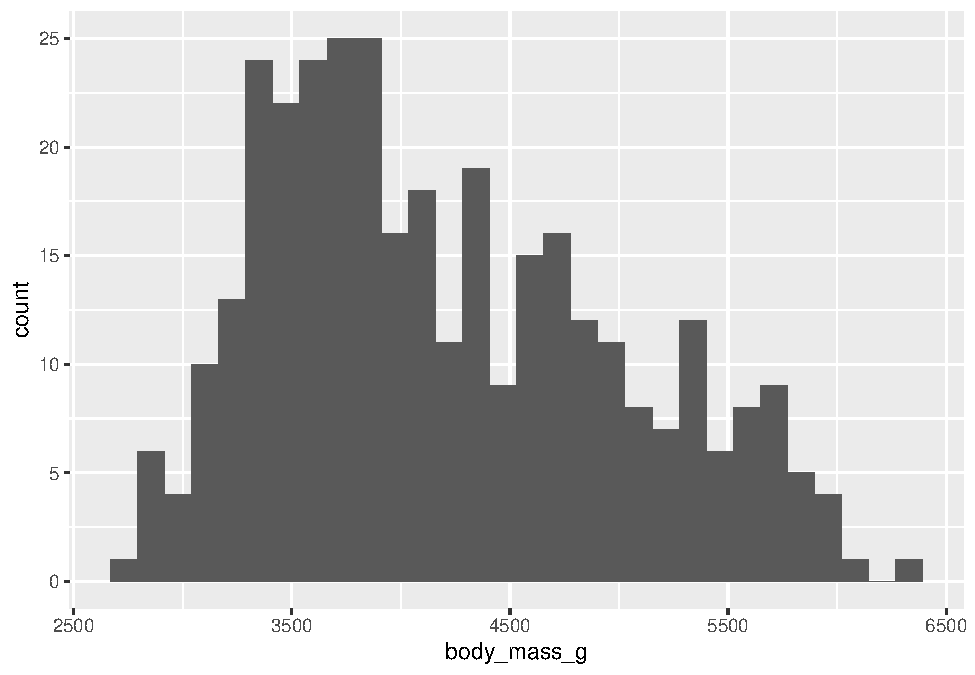
\includegraphics{intro_stats_files/figure-latex/unnamed-chunk-99-1.pdf}

\hypertarget{numerical-shape}{%
\subsection{The shape of data}\label{numerical-shape}}

The way histograms work is to create ``bins'', which are ranges of numbers along the x-axis. R goes through the data and counts how many observations fall into each bin. In that way, a histogram is somewhat like a bar chart. However, a bar chart uses bars to represent distinct, discrete categories, whereas a histogram uses bars that are all next to each other to represent values along a continuous numerical range. Histograms are meant to give you--at a quick glance--a sense of the ``shape'' of the data.

What do we mean by ``shape''? Generally, we look for three things:

\begin{enumerate}
\def\labelenumi{\arabic{enumi}.}
\tightlist
\item
  Modes
\end{enumerate}

\begin{itemize}
\tightlist
\item
  Modes are peaks in the data. These are places where data tends to cluster, representing common values of the numerical variable. In the \texttt{penguin} data, there appears to be a big mode between about 3500 and 4000 grams. When data has one clear mode, we call the data \emph{unimodal}. But data can also be \emph{bimodal}, or more generally, \emph{multimodal}. This often happens when the data contains multiple groups that are different from each other. In this case, we know there are three species of penguin in the data, so if those species are drastically different in their body mass, we might be looking at multimodal data. We'll explore this question more later in the chapter. For now, it's hard to say what's going on because the above histogram has a lot of spiky bars popping up all over. It's not completely obvious how many modes there might be.
\end{itemize}

\begin{enumerate}
\def\labelenumi{\arabic{enumi}.}
\setcounter{enumi}{1}
\tightlist
\item
  Symmetry
\end{enumerate}

\begin{itemize}
\tightlist
\item
  If there is one mode, we can also ask if the data is spread evenly to the left and right of that mode. If so, we call the data \emph{symmetric}. No data is perfectly symmetric, but we are looking for overall balance between the areas to the left and right of the mode. When data is not symmetric, we call is \emph{skewed}. Assuming that there is one big mode around 3500 or 4000, the body mass data above is skewed. There is clearly more data above the mode than below the mode. The right side of the histogram stretches out further to the right of the mode than to the left. Therefore, the body mass data is \emph{right-skewed}. There is a longer ``tail'' to the right. If it were the opposite, it would be \emph{left-skewed}. It is common for beginning students to confuse these two terms. Be aware that we are not concerned about where the mode is. We want to know which side has more data spread into a longer tail. That is the direction of the skewness.
\end{itemize}

\begin{enumerate}
\def\labelenumi{\arabic{enumi}.}
\setcounter{enumi}{2}
\tightlist
\item
  Outliers.
\end{enumerate}

\begin{itemize}
\tightlist
\item
  Outliers are data points that are far from the bulk of the data. The body mass data above appears to have no outliers. We are looking for a large gap between the main ``mass'' of data and any lingering data points far away from that mass. There is no such large gap in the histogram above.
\end{itemize}

\textbf{Whenever you are asked about the ``shape'' of a numerical variable, be sure to comment on (1) modes, (2) symmetry, and (3) outliers.}

Generally, the default binning for \texttt{ggplot} histograms is not great. This is by design. The creator of the \texttt{gglot2} package, Hadley Wickham, said the following:

\begin{quote}
``In ggplot2, a very simple heuristic is used for the default number of bins: it uses 30, regardless of the data. This is perverse, and ignores all of the research on selecting good bin sizes automatically, but sends a clear message to the user that he or she needs to think about, and experiment with, the bin width. This message is reinforced with a warning that reminds the user to manually adjust the bin width.''
\end{quote}

Indeed, if you look at the output from the graphing command above, you can see that \texttt{ggplot} informs you that you should pick a better value for the binwidth. You can also see that the bins aren't ideal. They are too narrow, which means that arbitrary differences between bins show up as ``random'' spikes all over the graph. These spikes can confuse the issue of how many modes appear in the data.

Instead, we should aim to use bins that show the overall shape of the data and smooth it out a bit. Look back at the scale of the x-axis to assess how wide each bar should be. There's no one correct answer. In this case, the bins ought to be a little wider. Since our x-axis goes from about 2500 to 6500, maybe we should try a binwidth of 250. And if 250 doesn't look good, nothing prevents us from trying a different number.

It's also easier to interpret the histogram when the bins' edges line up with numbers that are easy to see in the plot. Use \texttt{boundary} to determine where you want the bin boundaries to fall. For example, if we set the boundary to 3500, that means that one bar will start with its left edge at 3500. This is convenient because there is a tick mark labeled there on the x-axis. The boundary number is pretty arbitrary; once one boundary is set, it determines where all the other bins will line up. With a binwidth of 250, we'd get the same graph if the boundary were set to 3000 or 3250 or 5750, or even 0. Any other multiple of 250 would give the same graph.

We use \texttt{binwidth} and \texttt{boundary} inside the parentheses of the \texttt{geom\_histogram} to modify these parameters.

\begin{Shaded}
\begin{Highlighting}[]
\FunctionTok{ggplot}\NormalTok{(penguins, }\FunctionTok{aes}\NormalTok{(}\AttributeTok{x =}\NormalTok{ body\_mass\_g)) }\SpecialCharTok{+}
    \FunctionTok{geom\_histogram}\NormalTok{(}\AttributeTok{binwidth =} \DecValTok{250}\NormalTok{, }\AttributeTok{boundary =} \DecValTok{3500}\NormalTok{)}
\end{Highlighting}
\end{Shaded}

\begin{verbatim}
## Warning: Removed 2 rows containing non-finite values (stat_bin).
\end{verbatim}

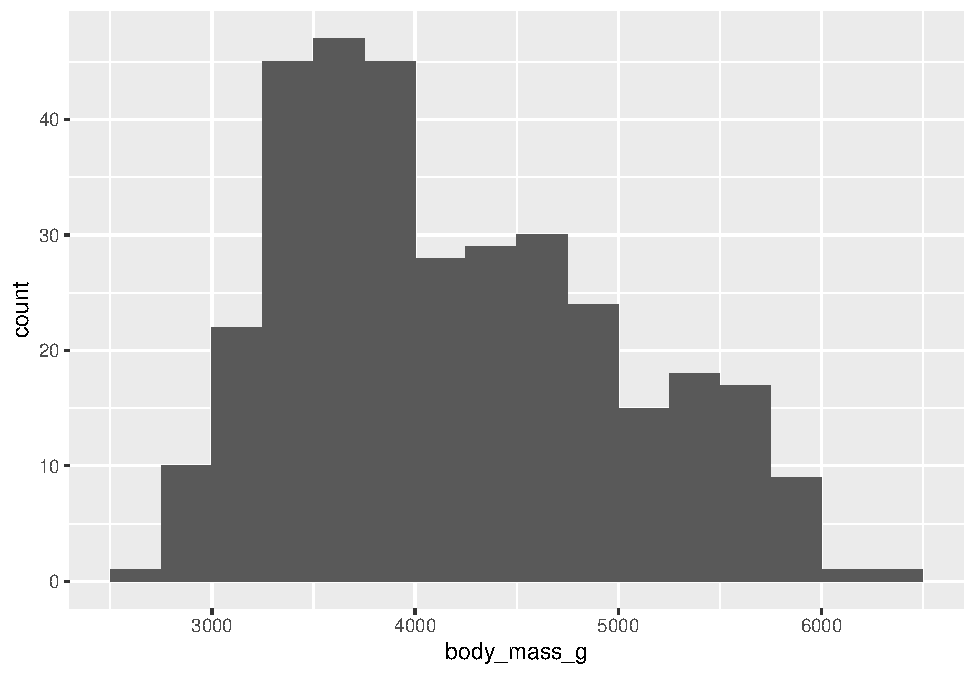
\includegraphics{intro_stats_files/figure-latex/unnamed-chunk-100-1.pdf}

Even with the smoother look, it appears that there are multiple modes, maybe three? Do these correspond to the three species of penguin? Stay tuned.

\hypertarget{exercise-6a-1}{%
\paragraph*{Exercise 6(a)}\label{exercise-6a-1}}
\addcontentsline{toc}{paragraph}{Exercise 6(a)}

Here is a histogram of the penguin bill lengths (measured in millimeters):

\begin{Shaded}
\begin{Highlighting}[]
\FunctionTok{ggplot}\NormalTok{(penguins, }\FunctionTok{aes}\NormalTok{(}\AttributeTok{x =}\NormalTok{ bill\_length\_mm)) }\SpecialCharTok{+}
    \FunctionTok{geom\_histogram}\NormalTok{(}\AttributeTok{binwidth =} \DecValTok{6}\NormalTok{, }\AttributeTok{boundary =} \DecValTok{30}\NormalTok{)}
\end{Highlighting}
\end{Shaded}

\begin{verbatim}
## Warning: Removed 2 rows containing non-finite values (stat_bin).
\end{verbatim}

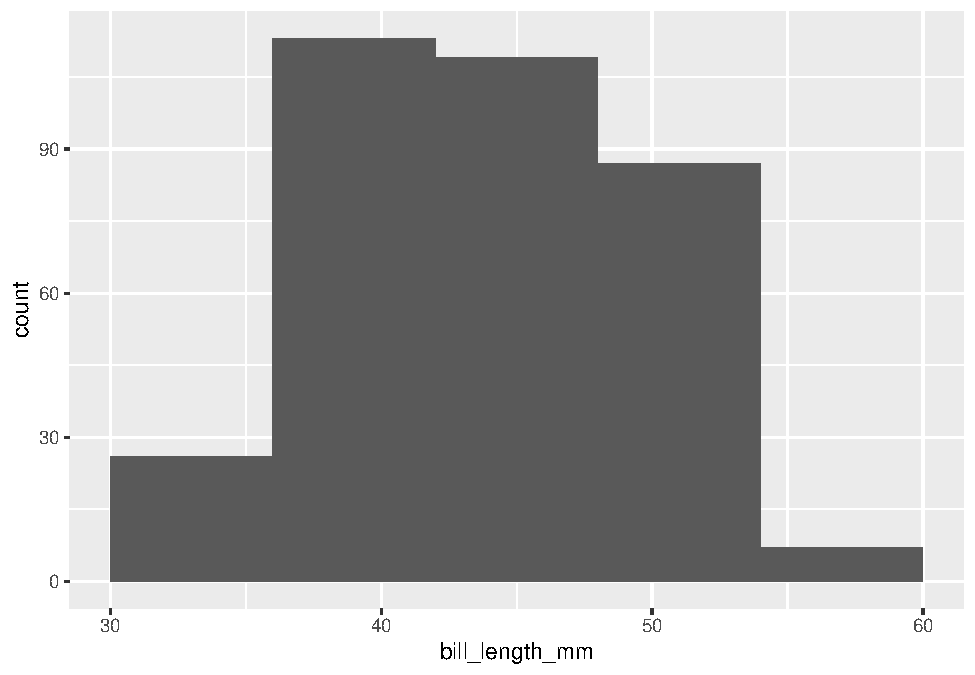
\includegraphics{intro_stats_files/figure-latex/unnamed-chunk-101-1.pdf}

Write a short paragraph describing the shape of the distribution of penguin bill lengths, focusing on the three key shape features (modes, symmetry, and outliers).

Please write up your answer here.

\hypertarget{exercise-6b-1}{%
\paragraph*{Exercise 6(b)}\label{exercise-6b-1}}
\addcontentsline{toc}{paragraph}{Exercise 6(b)}

The last question was a trick question!

Change the binwidth (no need to change the boundary) to something smaller to see more clearly the bimodal nature of the distribution.

\begin{Shaded}
\begin{Highlighting}[]
\CommentTok{\# Add code here that changes the binwidth of the last histogram to see}
\CommentTok{\# the bimodal nature of the distribution.}
\end{Highlighting}
\end{Shaded}

\hypertarget{exercise-7a-1}{%
\paragraph*{Exercise 7(a)}\label{exercise-7a-1}}
\addcontentsline{toc}{paragraph}{Exercise 7(a)}

Make a histogram of the variable \texttt{flipper\_length\_mm}. Start with a histogram where you don't modify the binwidth or boundary.

\begin{Shaded}
\begin{Highlighting}[]
\CommentTok{\# Add code here to create a histogram of flipper length}
\end{Highlighting}
\end{Shaded}

\hypertarget{exercise-7b-1}{%
\paragraph*{Exercise 7(b)}\label{exercise-7b-1}}
\addcontentsline{toc}{paragraph}{Exercise 7(b)}

By examining the scale on the x-axis above, repeat the command, but this time change the binwidth and the boundary until you are satisfied that the bins are neither too wide nor too narrow.

\begin{Shaded}
\begin{Highlighting}[]
\CommentTok{\# Add code here to modify the histogram of flipper length,}
\CommentTok{\# adding binwidth and boundary}
\end{Highlighting}
\end{Shaded}

\hypertarget{exercise-7c-1}{%
\paragraph*{Exercise 7(c)}\label{exercise-7c-1}}
\addcontentsline{toc}{paragraph}{Exercise 7(c)}

Write a short paragraph describing the shape of the distribution of penguin flipper lengths, focusing on the three key shape features (modes, symmetry, and outliers).

Please write up your answer here.

\hypertarget{numerical-less-useful}{%
\subsection{Less useful plot types}\label{numerical-less-useful}}

There are several other graph types that one might see for a single numerical variable: e.g., dotplots, stem-and-leaf plots, boxplots, etc. I'm not a big fan of dotplots or stem-and-leaf plots as they are just messier versions of histograms. I do like boxplots, but they are typically less informative than histograms. Boxplots are much better for comparing groups, and we'll see them later in the chapter.

\hypertarget{numerical-graphing-two}{%
\section{Graphing two numerical variables}\label{numerical-graphing-two}}

The proper graph for two numerical variables is a scatterplot. We graph the response variable on the y-axis and the predictor variable on the x-axis.

Let's consider a possible association between bill length and body mass. For this question, there is not really a strong preference for which variable serves as response and which variable servers as predictor. We'll consider bill length as the response variable and body mass as the predictor.

Since we are plotting two variables, we have two aesthetics, one on the y-axis (the response variable) and one on the x-axis (the predictor variable). Since scatterplots use points to plot each data value, the correct layer to add is \texttt{geom\_point()}.

\begin{Shaded}
\begin{Highlighting}[]
\FunctionTok{ggplot}\NormalTok{(penguins, }\FunctionTok{aes}\NormalTok{(}\AttributeTok{y =}\NormalTok{ bill\_length\_mm, }\AttributeTok{x =}\NormalTok{ body\_mass\_g)) }\SpecialCharTok{+}
    \FunctionTok{geom\_point}\NormalTok{()}
\end{Highlighting}
\end{Shaded}

\begin{verbatim}
## Warning: Removed 2 rows containing missing values (geom_point).
\end{verbatim}

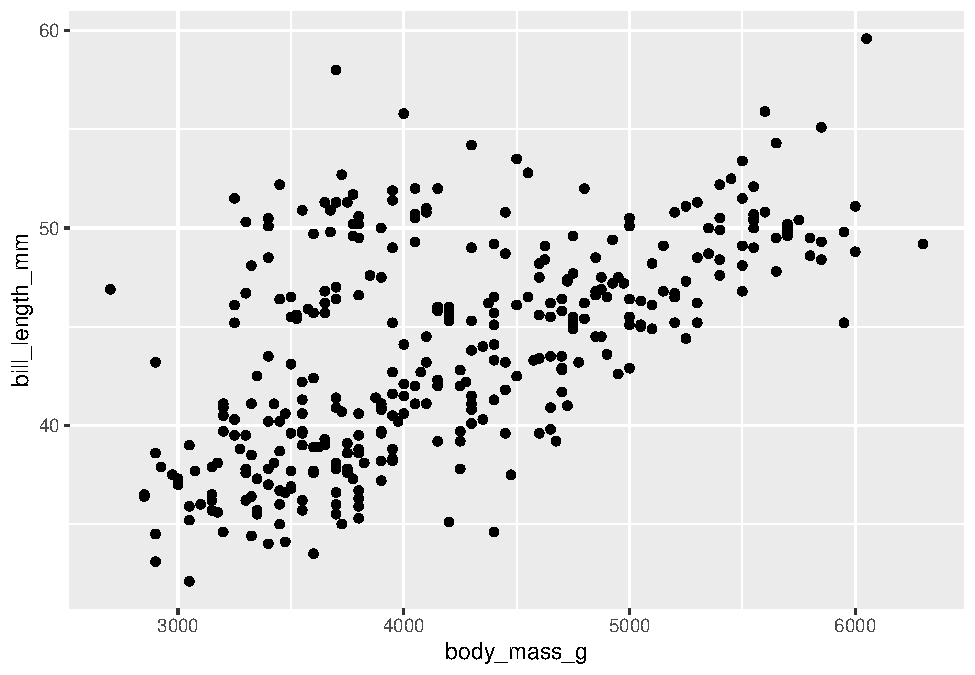
\includegraphics{intro_stats_files/figure-latex/unnamed-chunk-105-1.pdf}

We are looking for evidence of a relationship between the two variables. This will manifest as a pattern in the data. We are interested in answering the following questions:

\begin{enumerate}
\def\labelenumi{\arabic{enumi}.}
\tightlist
\item
  Linearity
\end{enumerate}

\begin{itemize}
\tightlist
\item
  Is the association linear? In other words, do the data points lie roughly in a straight line pattern? The scatterplot above is a bit ``cloudy'' but generally moves from lower left to upper right in a straight (not curved pattern). It's not a completely random scatter of dots.
\end{itemize}

\begin{enumerate}
\def\labelenumi{\arabic{enumi}.}
\setcounter{enumi}{1}
\tightlist
\item
  Direction
\end{enumerate}

\begin{itemize}
\tightlist
\item
  If the pattern is linear, it is a \emph{positive} relationship or a \emph{negative} one? Positive means that the line moves from lower left to upper right. Negative means it moves from upper left to lower right. If you recall the direction of slopes from high school algebra class, a positive association corresponds to a line with a positive slope, and similarly for a negative association. In the data above, lower values of body mass correspond to lower bill lengths, and higher values of body mass correspond to higher bill lengths. So this is a positive association.
\end{itemize}

\begin{enumerate}
\def\labelenumi{\arabic{enumi}.}
\setcounter{enumi}{2}
\tightlist
\item
  Strength
\end{enumerate}

\begin{itemize}
\tightlist
\item
  If there is a pattern, how tight is the pattern? Do the data points stay close to a straight line, or are they pretty spread out and only generally moving in one direction. A strong relationship is one that is tightly packed around a line or curve. The relationship above is not strong. We might use terms like ``weak'', ``moderately weak'', or ``moderate'', but definitely not strong.
\end{itemize}

\begin{enumerate}
\def\labelenumi{\arabic{enumi}.}
\setcounter{enumi}{3}
\tightlist
\item
  Outliers
\end{enumerate}

\begin{itemize}
\tightlist
\item
  Are there outliers? These will be points that are isolated and relatively far from the bulk of the data. There are a few points above that are borderline, but none is a particularly strong outlier, especially give how spread out the rest of the data is.
\end{itemize}

\hypertarget{exercise-8}{%
\paragraph*{Exercise 8}\label{exercise-8}}
\addcontentsline{toc}{paragraph}{Exercise 8}

Here is a scatterplot of

\begin{Shaded}
\begin{Highlighting}[]
\FunctionTok{ggplot}\NormalTok{(penguins, }\FunctionTok{aes}\NormalTok{(}\AttributeTok{y =}\NormalTok{ flipper\_length\_mm, }\AttributeTok{x =}\NormalTok{ body\_mass\_g)) }\SpecialCharTok{+}
    \FunctionTok{geom\_point}\NormalTok{()}
\end{Highlighting}
\end{Shaded}

\begin{verbatim}
## Warning: Removed 2 rows containing missing values (geom_point).
\end{verbatim}

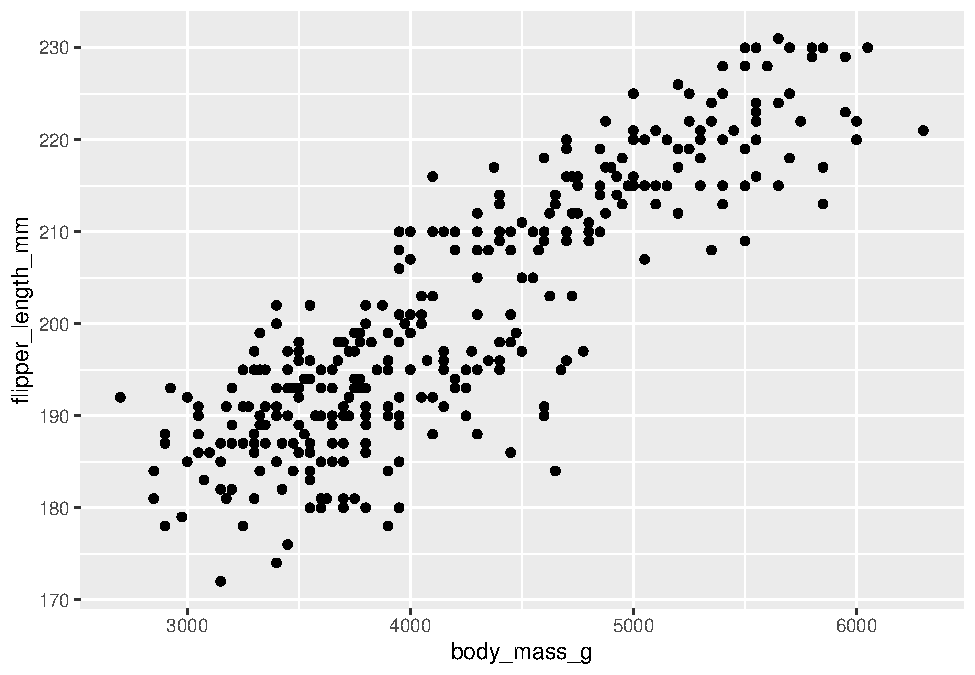
\includegraphics{intro_stats_files/figure-latex/unnamed-chunk-106-1.pdf}

Write a short paragraph describing the association of penguin flipper lengths and body mass, focusing on the four key features (linearity, direction, strength, and outliers).

Please write up your answer here.

\hypertarget{numerical-graphing-grouped}{%
\section{Graphing grouped numerical data}\label{numerical-graphing-grouped}}

Suppose you want to analyze one numerical variable and one categorical variable. Usually, the idea here is that the categorical variable divides up the data into groups and you are interested in understanding the numerical variable for each group separately. Another way to say this is that your numerical variable is response and your categorical variable is predictor. (It is also possible for a categorical variable to be response and a numerical variable to be predictor. This is common in so-called ``classification'' problems. We will not cover this possibility in this course, but it is covered in more advanced courses.)

This turns out to be exactly what we need in the penguins data. Throughout the above exercises, there was a concern that the penguin measurements are fundamentally different among three different species of penguin.

Graphically, there are two good options here. The first is a side-by-side boxplot.

\begin{Shaded}
\begin{Highlighting}[]
\FunctionTok{ggplot}\NormalTok{(penguins, }\FunctionTok{aes}\NormalTok{(}\AttributeTok{y =}\NormalTok{ body\_mass\_g, }\AttributeTok{x =}\NormalTok{ species)) }\SpecialCharTok{+}
    \FunctionTok{geom\_boxplot}\NormalTok{()}
\end{Highlighting}
\end{Shaded}

\begin{verbatim}
## Warning: Removed 2 rows containing non-finite values (stat_boxplot).
\end{verbatim}

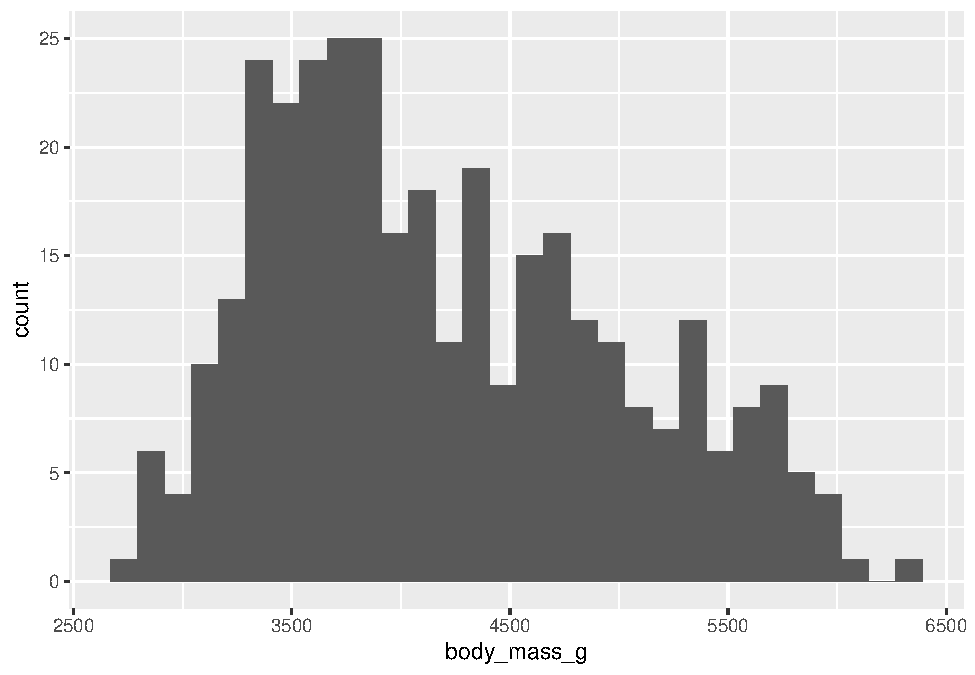
\includegraphics{intro_stats_files/figure-latex/unnamed-chunk-107-1.pdf}

Notice the placement of the variables. The y-axis is \texttt{body\_mass\_g}, the numerical variable. The x-axis variable is \texttt{species}; the groups are placed along the x-axis. This is consistent with other graph types that place the response variable on the y-axis and the predictor variable on the x-axis.

The other possible graph is a stacked histogram. This uses a feature called ``faceting'' that creates a different plot for each group. The syntax is a little unusual.

\begin{Shaded}
\begin{Highlighting}[]
\FunctionTok{ggplot}\NormalTok{(penguins, }\FunctionTok{aes}\NormalTok{(}\AttributeTok{x =}\NormalTok{ body\_mass\_g)) }\SpecialCharTok{+}
    \FunctionTok{geom\_histogram}\NormalTok{() }\SpecialCharTok{+}
    \FunctionTok{facet\_grid}\NormalTok{(species }\SpecialCharTok{\textasciitilde{}}\NormalTok{ .)}
\end{Highlighting}
\end{Shaded}

\begin{verbatim}
## `stat_bin()` using `bins = 30`. Pick better value with `binwidth`.
\end{verbatim}

\begin{verbatim}
## Warning: Removed 2 rows containing non-finite values (stat_bin).
\end{verbatim}

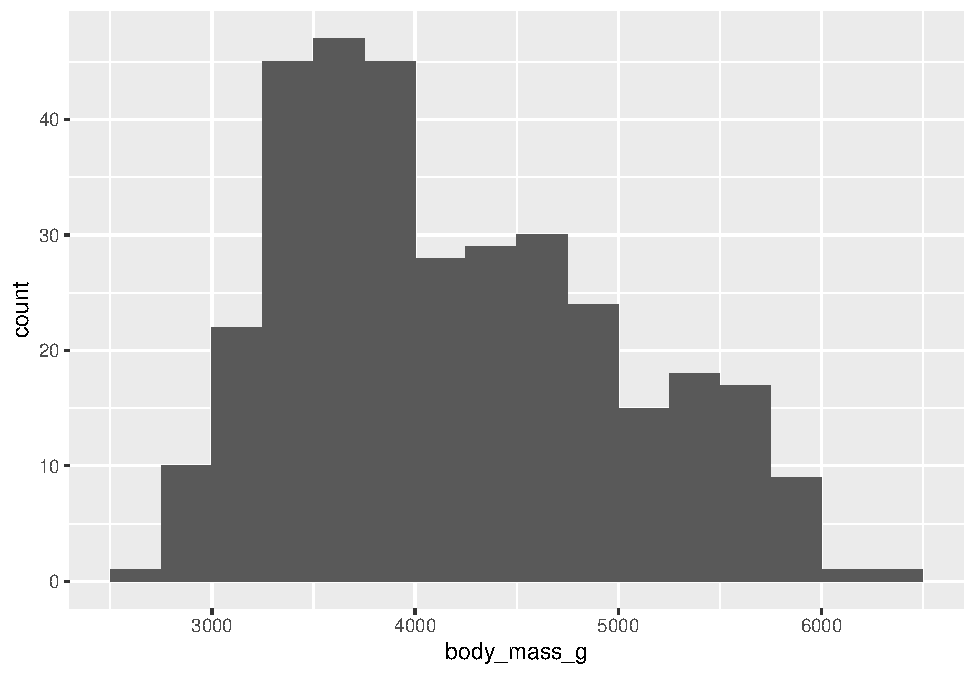
\includegraphics{intro_stats_files/figure-latex/unnamed-chunk-108-1.pdf}

The argument \texttt{species\ \textasciitilde{}\ .} in the \texttt{facet\_grid} function means, ``Put each species on a different row.'' We'll explore this notation a little later.

As always, the default bins suck, so let's change them.

\begin{Shaded}
\begin{Highlighting}[]
\FunctionTok{ggplot}\NormalTok{(penguins, }\FunctionTok{aes}\NormalTok{(}\AttributeTok{x =}\NormalTok{ body\_mass\_g)) }\SpecialCharTok{+}
    \FunctionTok{geom\_histogram}\NormalTok{(}\AttributeTok{binwidth =} \DecValTok{250}\NormalTok{, }\AttributeTok{boundary =} \DecValTok{3500}\NormalTok{) }\SpecialCharTok{+}
    \FunctionTok{facet\_grid}\NormalTok{(species }\SpecialCharTok{\textasciitilde{}}\NormalTok{ .)}
\end{Highlighting}
\end{Shaded}

\begin{verbatim}
## Warning: Removed 2 rows containing non-finite values (stat_bin).
\end{verbatim}

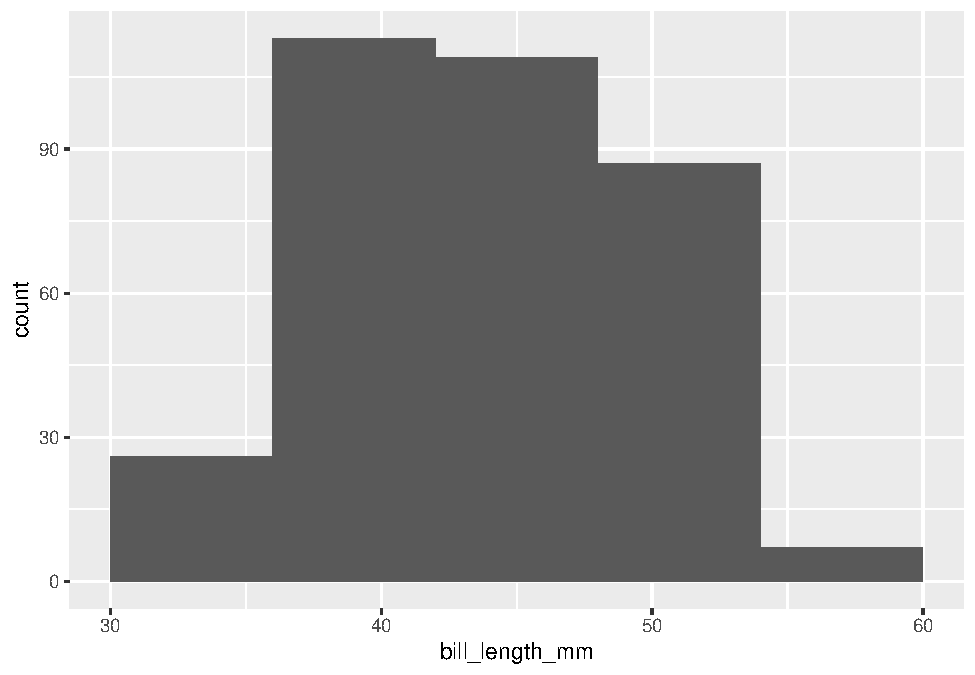
\includegraphics{intro_stats_files/figure-latex/unnamed-chunk-109-1.pdf}

Consider the following subtle change in notation:

\begin{Shaded}
\begin{Highlighting}[]
\FunctionTok{ggplot}\NormalTok{(penguins, }\FunctionTok{aes}\NormalTok{(}\AttributeTok{x =}\NormalTok{ body\_mass\_g)) }\SpecialCharTok{+}
    \FunctionTok{geom\_histogram}\NormalTok{(}\AttributeTok{binwidth =} \DecValTok{250}\NormalTok{, }\AttributeTok{boundary =} \DecValTok{3500}\NormalTok{) }\SpecialCharTok{+}
    \FunctionTok{facet\_grid}\NormalTok{(. }\SpecialCharTok{\textasciitilde{}}\NormalTok{ species)}
\end{Highlighting}
\end{Shaded}

\begin{verbatim}
## Warning: Removed 2 rows containing non-finite values (stat_bin).
\end{verbatim}

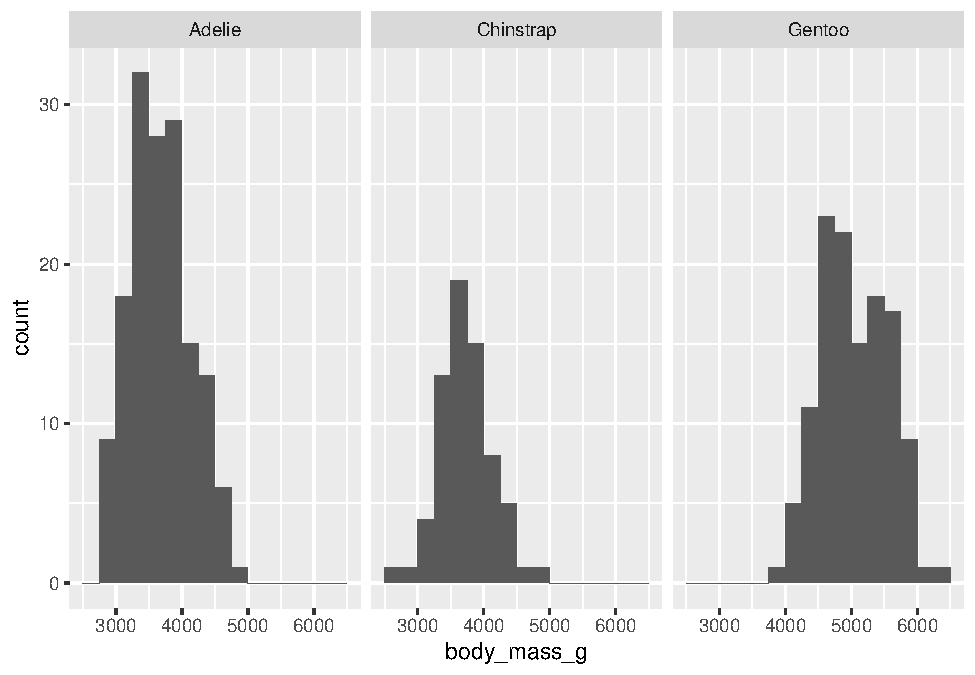
\includegraphics{intro_stats_files/figure-latex/unnamed-chunk-110-1.pdf}

\hypertarget{exercise-9a-1}{%
\paragraph*{Exercise 9(a)}\label{exercise-9a-1}}
\addcontentsline{toc}{paragraph}{Exercise 9(a)}

Explain why that last graph (which might be called a side-by-side histogram) is less effective than the earlier stacked histogram. (Hint: what stays lined up when the histograms are stacked vertically rather than horizontally?)

Please write up your answer here.

\hypertarget{exercise-9b-1}{%
\paragraph*{Exercise 9(b)}\label{exercise-9b-1}}
\addcontentsline{toc}{paragraph}{Exercise 9(b)}

Can you figure out what's going on with the weird syntax of \texttt{species\ \textasciitilde{}\ .} vs \texttt{.\ \textasciitilde{}\ species}? Explain it in your own words.

Please write up your answer here.

\begin{center}\rule{0.5\linewidth}{0.5pt}\end{center}

The other thing that kind of sucks is the fact that the y-axis is showing counts. That makes it harder to see the distribution of body mass among Chinstrap penguins, for example, as there are fewer of them in the data set. It would be nice to scale these using percentages.

\begin{Shaded}
\begin{Highlighting}[]
\FunctionTok{ggplot}\NormalTok{(penguins, }\FunctionTok{aes}\NormalTok{(}\AttributeTok{x =}\NormalTok{ body\_mass\_g)) }\SpecialCharTok{+}
    \FunctionTok{geom\_histogram}\NormalTok{(}\FunctionTok{aes}\NormalTok{(}\AttributeTok{y =}\NormalTok{ ..density..),}
                   \AttributeTok{binwidth =} \DecValTok{250}\NormalTok{, }\AttributeTok{boundary =} \DecValTok{3500}\NormalTok{) }\SpecialCharTok{+}
    \FunctionTok{facet\_grid}\NormalTok{(species }\SpecialCharTok{\textasciitilde{}}\NormalTok{ .)}
\end{Highlighting}
\end{Shaded}

\begin{verbatim}
## Warning: Removed 2 rows containing non-finite values (stat_bin).
\end{verbatim}

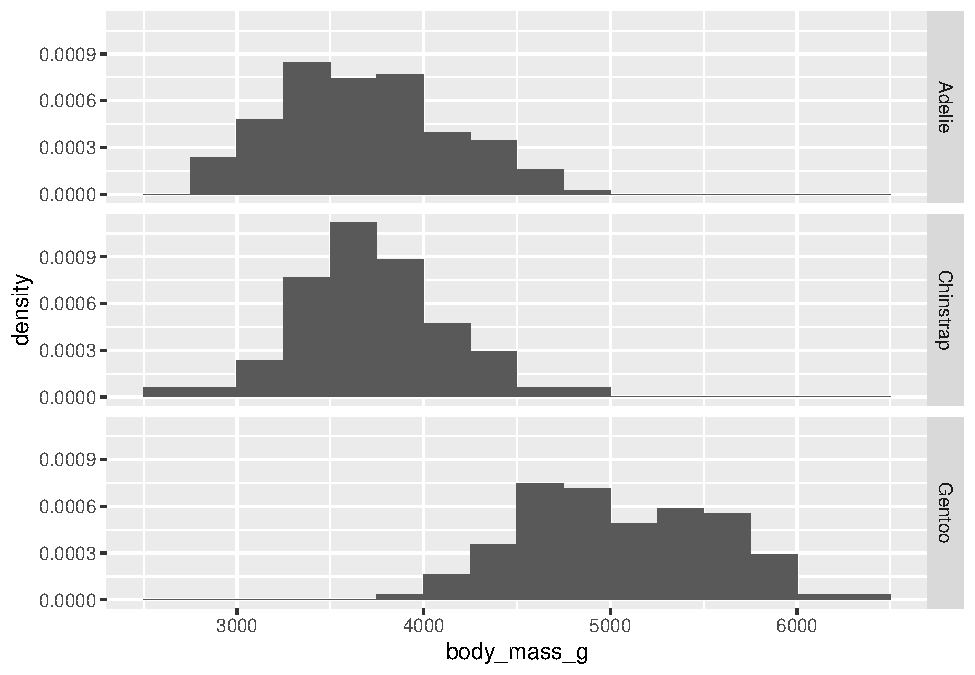
\includegraphics{intro_stats_files/figure-latex/unnamed-chunk-111-1.pdf}

Due to some technical issues in \texttt{ggplot2}, these are not strictly proportions. (If you were to add up the heights of all the bars, they would not add up to 100\%.) Nevertheless, the graph is still useful because it does scale the groups to put them on equal footing. In other words, it treats each group as if they all had the same sample size.

\hypertarget{exercise-10}{%
\paragraph*{Exercise 10}\label{exercise-10}}
\addcontentsline{toc}{paragraph}{Exercise 10}

Choose a numerical variable that's not body mass and a categorical variable that's not species from the \texttt{penguins} data set. Make both a side-by-side boxplot and a stacked histogram. Discuss the resulting graphs. Comment on the association (or independence) of the two variables. If there is an association, be sure to focus on the four key features (linearity, direction, strength, and outliers).

\begin{Shaded}
\begin{Highlighting}[]
\CommentTok{\# Add code here to create a side{-}by{-}side boxplot.}
\end{Highlighting}
\end{Shaded}

\begin{Shaded}
\begin{Highlighting}[]
\CommentTok{\# Add code here to create a stacked histogram.}
\end{Highlighting}
\end{Shaded}

Please write up your answer here.

\hypertarget{numerical-pub}{%
\section{Publication-ready graphics}\label{numerical-pub}}

The great thing about \texttt{ggplot2} graphics is that they are already quite pretty. To take them from exploratory data analysis to the next level, there are a few things we can do to tidy them up.

Let's go back to the first histogram from this chapter.

\begin{Shaded}
\begin{Highlighting}[]
\FunctionTok{ggplot}\NormalTok{(penguins, }\FunctionTok{aes}\NormalTok{(}\AttributeTok{x =}\NormalTok{ body\_mass\_g)) }\SpecialCharTok{+}
    \FunctionTok{geom\_histogram}\NormalTok{(}\AttributeTok{binwidth =} \DecValTok{250}\NormalTok{, }\AttributeTok{boundary =} \DecValTok{3500}\NormalTok{)}
\end{Highlighting}
\end{Shaded}

\begin{verbatim}
## Warning: Removed 2 rows containing non-finite values (stat_bin).
\end{verbatim}

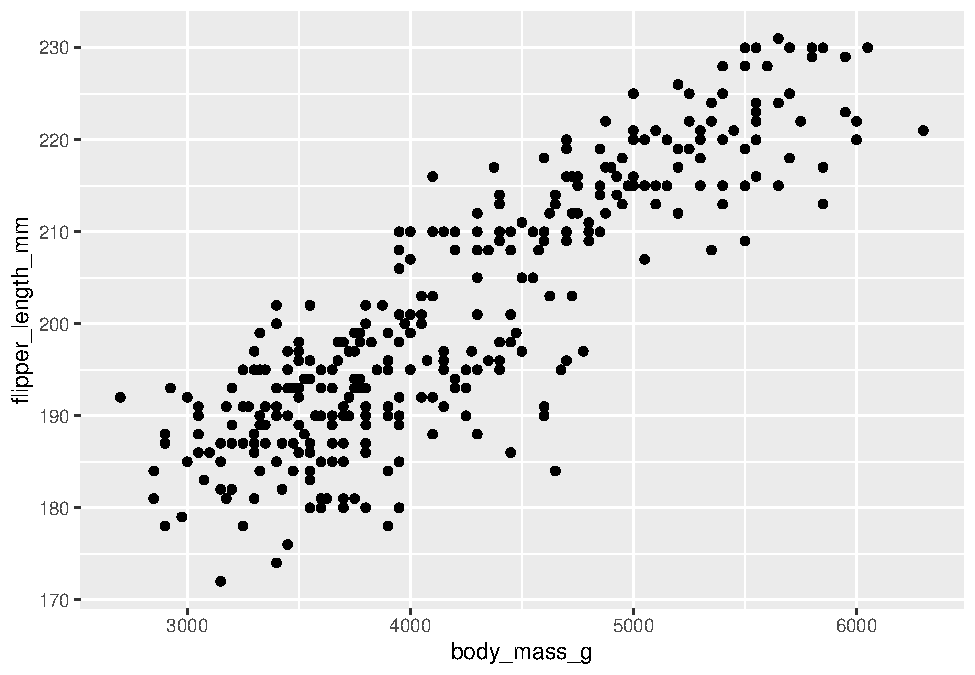
\includegraphics{intro_stats_files/figure-latex/unnamed-chunk-114-1.pdf}

The variable names of this data set are already pretty informative, but we can do a little better with \texttt{labs} (for labels). Observe:

\begin{Shaded}
\begin{Highlighting}[]
\FunctionTok{ggplot}\NormalTok{(penguins, }\FunctionTok{aes}\NormalTok{(}\AttributeTok{x =}\NormalTok{ body\_mass\_g)) }\SpecialCharTok{+}
    \FunctionTok{geom\_histogram}\NormalTok{(}\AttributeTok{binwidth =} \DecValTok{250}\NormalTok{, }\AttributeTok{boundary =} \DecValTok{3500}\NormalTok{) }\SpecialCharTok{+}
    \FunctionTok{labs}\NormalTok{(}\AttributeTok{title =} \StringTok{"Distribution of body mass for adult foraging penguins near}
\StringTok{         Palmer Station, Antarctica"}\NormalTok{,}
         \AttributeTok{x =} \StringTok{"Body mass (in grams)"}\NormalTok{,}
         \AttributeTok{y =} \StringTok{"Count"}\NormalTok{)}
\end{Highlighting}
\end{Shaded}

\begin{verbatim}
## Warning: Removed 2 rows containing non-finite values (stat_bin).
\end{verbatim}

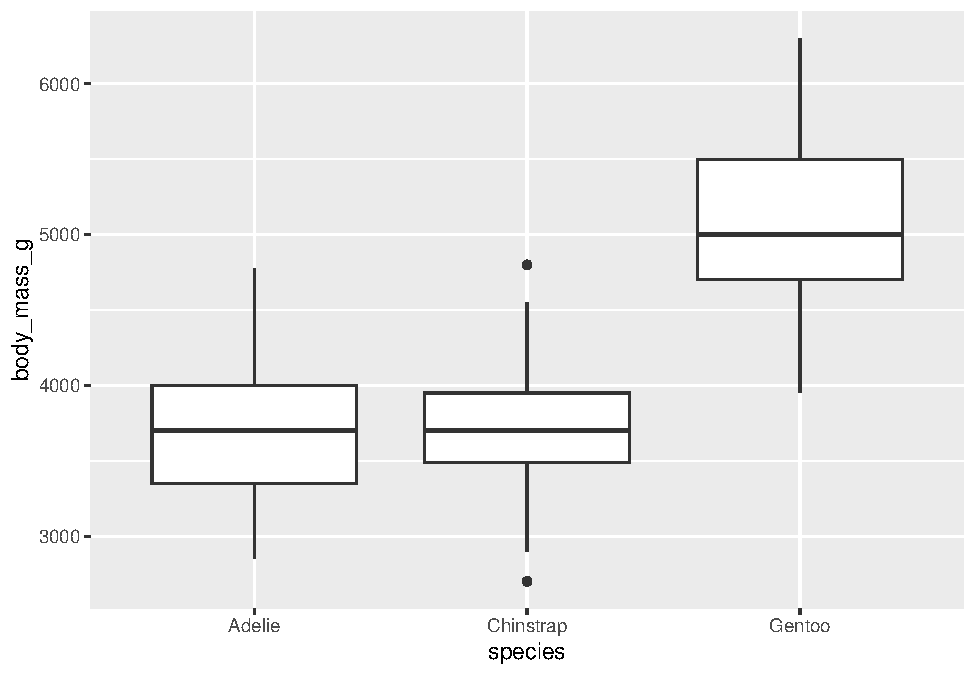
\includegraphics{intro_stats_files/figure-latex/unnamed-chunk-115-1.pdf}

You can also see that we took the opportunity to mention the units of measurement (grams) for our variable in the x-axis label. This is good practice.

A quick note about formatting in R code chunks. Notice that I put different parts of the last \texttt{ggplot} command on their own separate lines. The command would still work if I did this:

\begin{Shaded}
\begin{Highlighting}[]
\FunctionTok{ggplot}\NormalTok{(penguins, }\FunctionTok{aes}\NormalTok{(}\AttributeTok{x =}\NormalTok{ body\_mass\_g)) }\SpecialCharTok{+} \FunctionTok{geom\_histogram}\NormalTok{(}\AttributeTok{binwidth =} \DecValTok{250}\NormalTok{, }\AttributeTok{boundary =} \DecValTok{3500}\NormalTok{) }\SpecialCharTok{+} \FunctionTok{labs}\NormalTok{(}\AttributeTok{title =} \StringTok{"Distribution of body mass for adult foraging penguins near Palmer Station, Antarctica"}\NormalTok{, }\AttributeTok{x =} \StringTok{"Body mass (in grams)"}\NormalTok{, }\AttributeTok{y =} \StringTok{"Count"}\NormalTok{)}
\end{Highlighting}
\end{Shaded}

\begin{verbatim}
## Warning: Removed 2 rows containing non-finite values (stat_bin).
\end{verbatim}

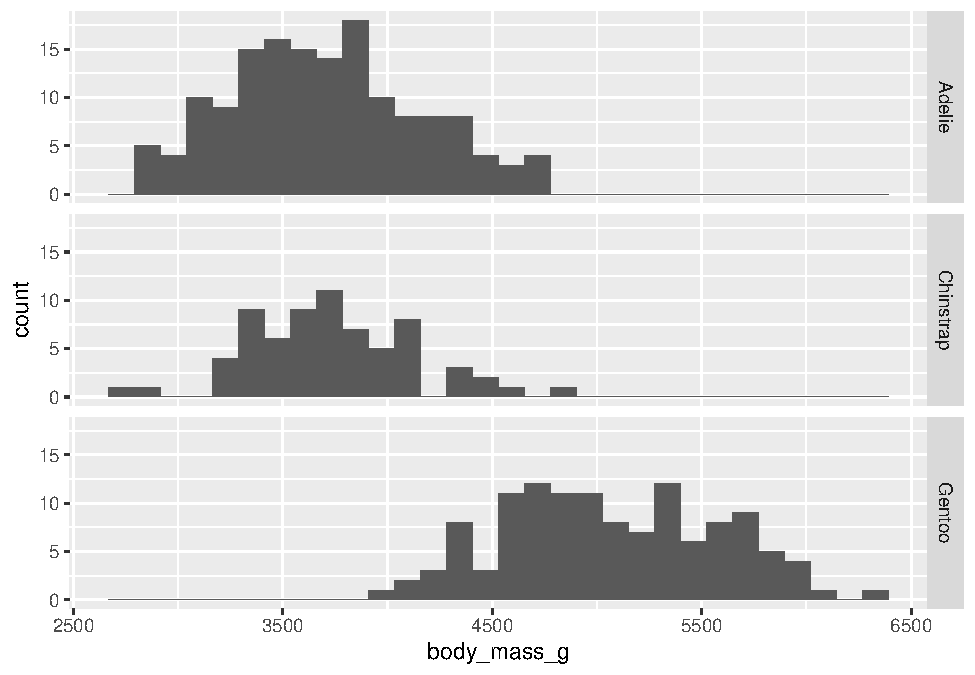
\includegraphics{intro_stats_files/figure-latex/unnamed-chunk-116-1.pdf}

But it's much harder to read. If you find that your code is ``wrapping'' to the next line, find some spots like commas or plus signs to break the code. Be sure to break the line after the comma or plus sign.

\hypertarget{exercise-11-1}{%
\paragraph*{Exercise 11}\label{exercise-11-1}}
\addcontentsline{toc}{paragraph}{Exercise 11}

Modify the following scatterplot by adding a title and labels for both the y-axis and x-axis.

\begin{Shaded}
\begin{Highlighting}[]
\CommentTok{\# Modify the following scatterplot by adding a title and }
\CommentTok{\# labels for both the y{-}axis and x{-}axis.}
\FunctionTok{ggplot}\NormalTok{(penguins, }\FunctionTok{aes}\NormalTok{(}\AttributeTok{y =}\NormalTok{ bill\_length\_mm, }\AttributeTok{x =}\NormalTok{ bill\_depth\_mm)) }\SpecialCharTok{+}
    \FunctionTok{geom\_point}\NormalTok{()}
\end{Highlighting}
\end{Shaded}

\begin{verbatim}
## Warning: Removed 2 rows containing missing values (geom_point).
\end{verbatim}

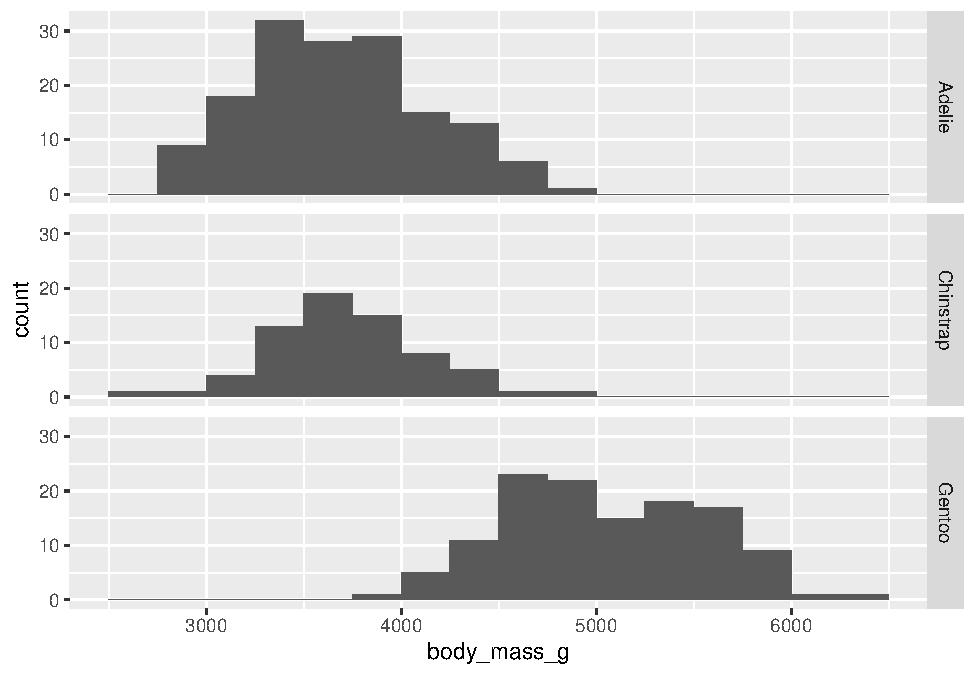
\includegraphics{intro_stats_files/figure-latex/unnamed-chunk-117-1.pdf}

\hypertarget{exercise-12-1}{%
\paragraph*{Exercise 12}\label{exercise-12-1}}
\addcontentsline{toc}{paragraph}{Exercise 12}

The previous scatterplot looked a little funny due to some odd groupings that we suspect (as usual) might be due to multiple species being measures. Add a new aesthetic (so, inside the parentheses following \texttt{aes}) to the following code to assign \texttt{color\ =\ species}. Comment on what you see.

\begin{Shaded}
\begin{Highlighting}[]
\CommentTok{\# Modify the code below to add color = species}
\FunctionTok{ggplot}\NormalTok{(penguins, }\FunctionTok{aes}\NormalTok{(}\AttributeTok{y =}\NormalTok{ bill\_length\_mm, }\AttributeTok{x =}\NormalTok{ bill\_depth\_mm)) }\SpecialCharTok{+}
    \FunctionTok{geom\_point}\NormalTok{()}
\end{Highlighting}
\end{Shaded}

\begin{verbatim}
## Warning: Removed 2 rows containing missing values (geom_point).
\end{verbatim}

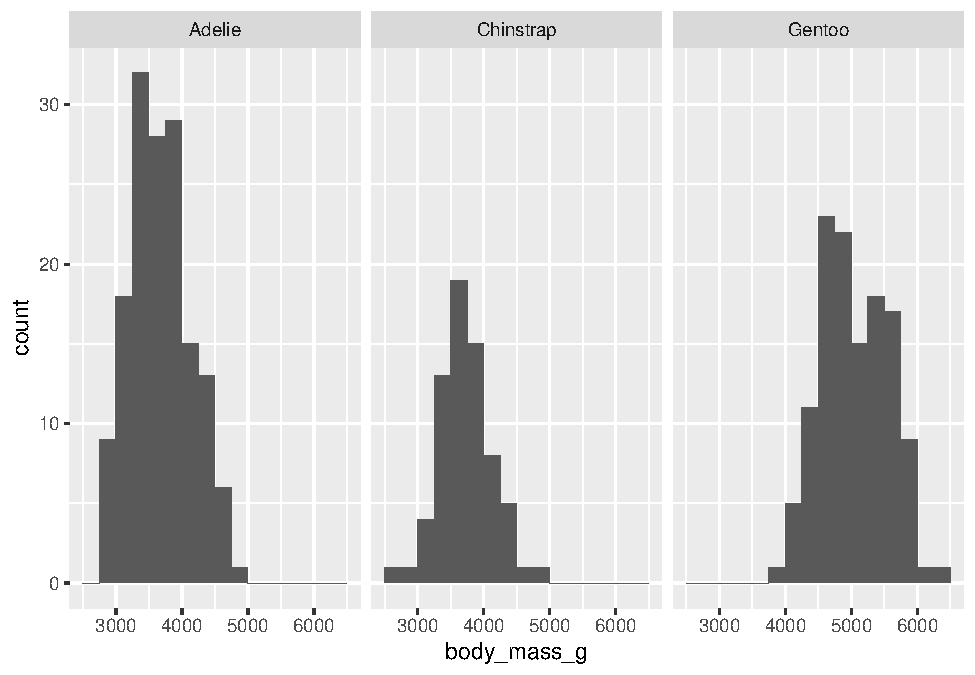
\includegraphics{intro_stats_files/figure-latex/unnamed-chunk-118-1.pdf}

Please write up your answer here.

\begin{center}\rule{0.5\linewidth}{0.5pt}\end{center}

Every part of the graph can be customized, from the color scheme to the tick marks on the axes, to the major and minor grid lines that appear on the background. We won't go into all that, but you can look at the \href{http://ggplot2.tidyverse.org/}{ggplot2 documentation} online and search Google for examples if you want to dig in and figure out how to do some of that stuff. However, the default options are often (but not always) the best, so be careful that your messing around doesn't inadvertently make the graph less clear or less appealing.

\hypertarget{numerical-conclusion}{%
\section{Conclusion}\label{numerical-conclusion}}

Summary statistics are simple numbers that describe and summarize data sets. Measures of center tell us where the ``middle'' of our numerical data lies, and measures of spread tell us how spread out our numerical data is. These measures should always be reported in pairs, for example the mean/standard deviation, or the median/IQR.

The \texttt{ggplot2} package with its \texttt{ggplot} command is a very versatile tool for creating nice graphs relatively easily. For a single numerical variable, the standard graph type is a histogram. For two numerical variables, use a scatterplot. For a numerical response with a categorical predictor, use either a side-by-side boxplot or a stacked histogram.

\hypertarget{numerical-prep}{%
\subsection{Preparing and submitting your assignment}\label{numerical-prep}}

\begin{enumerate}
\def\labelenumi{\arabic{enumi}.}
\tightlist
\item
  From the ``Run'' menu, select ``Restart R and Run All Chunks''.
\item
  Deal with any code errors that crop up. Repeat steps 1---2 until there are no more code errors.
\item
  Spell check your document by clicking the icon with ``ABC'' and a check mark.
\item
  Hit the ``Preview'' button one last time to generate the final draft of the \texttt{.nb.html} file.
\item
  Proofread the HTML file carefully. If there are errors, go back and fix them, then repeat steps 1--5 again.
\end{enumerate}

If you have completed this chapter as part of a statistics course, follow the directions you receive from your professor to submit your assignment.

\hypertarget{manipulating}{%
\chapter{Manipulating data}\label{manipulating}}

2.0

\hypertarget{functions-introduced-in-this-chapter-4}{%
\subsection*{Functions introduced in this chapter}\label{functions-introduced-in-this-chapter-4}}
\addcontentsline{toc}{subsection}{Functions introduced in this chapter}

\texttt{read\_csv}, \texttt{select}, \texttt{rename}, \texttt{rm}, \texttt{filter}, \texttt{slice}, \texttt{arrange}, \texttt{mutate}, \texttt{all.equal}, \texttt{ifelse}, \texttt{transmute}, \texttt{summarise}, \texttt{group\_by}, \texttt{\%\textgreater{}\%}, \texttt{count}

\hypertarget{manipulating-intro}{%
\section{Introduction}\label{manipulating-intro}}

This tutorial will import some data from the web and then explore it using the amazing \texttt{dplyr} package, a package which is quickly becoming the \emph{de facto} standard among R users for manipulating data. It's part of the \texttt{tidyverse} that we've already used in several chapters.

\hypertarget{manipulating-install}{%
\subsection{Install new packages}\label{manipulating-install}}

There are no new packages used in this chapter.

\hypertarget{manipulating-download}{%
\subsection{Download the R notebook file}\label{manipulating-download}}

Check the upper-right corner in RStudio to make sure you're in your \texttt{intro\_stats} project. Then click on the following link to download this chapter as an R notebook file (\texttt{.Rmd}).

https://vectorposse.github.io/intro\_stats/chapter\_downloads/05-manipulating\_data.Rmd

Once the file is downloaded, move it to your project folder in RStudio and open it there.

\hypertarget{manipulating-restart}{%
\subsection{Restart R and run all chunks}\label{manipulating-restart}}

In RStudio, select ``Restart R and Run All Chunks'' from the ``Run'' menu.

\hypertarget{manipulating-load}{%
\subsection{Load packages}\label{manipulating-load}}

We load the \texttt{tidyverse} package as usual, but this time it is to give us access to the \texttt{dplyr} package, which is loaded alongside our other \texttt{tidyverse} packages like \texttt{ggplot2}. The \texttt{tidyverse} also has a package called \texttt{readr} that will allow us to import data from an external source (in this case, a web site).

\begin{Shaded}
\begin{Highlighting}[]
\FunctionTok{library}\NormalTok{(tidyverse)}
\end{Highlighting}
\end{Shaded}

\hypertarget{manipulating-csv}{%
\section{Importing CSV data}\label{manipulating-csv}}

For most of the chapters, we use data sets that are either included in base R or included in a package that can be loaded into R. But it is useful to see how to get a data set from outside the R ecosystem. This depends a lot on the format of the data file, but a common format is a ``comma-separated values'' file, or CSV file. If you have a data set that is not formatted as a CSV file, it is usually pretty easy to open it in something like Google Spreadsheets or Microsoft Excel and then re-save it as a CSV file.

The file we'll import is a random sample from all the commercial domestic flights that departed from Houston, Texas, in 2011.

We use the \texttt{read\_csv} command to import a CSV file. In this case, we're grabbing the file from a web page where the file is hosted. If you have a file on your computer, you can also put the file into your project directory and import it from there. Put the URL (for a web page) or the filename (for a file in your project directory) in quotes inside the \texttt{read\_csv}command. We also need to assign the output to a tibble, so we've called it \texttt{hf} for ``Houston flights''.

\begin{Shaded}
\begin{Highlighting}[]
\NormalTok{hf }\OtherTok{\textless{}{-}} \FunctionTok{read\_csv}\NormalTok{(}\StringTok{"https://vectorposse.github.io/intro\_stats/data/hf.csv"}\NormalTok{)}
\end{Highlighting}
\end{Shaded}

\begin{verbatim}
## Rows: 22758 Columns: 21
## -- Column specification --------------------------------------------------------
## Delimiter: ","
## chr  (5): UniqueCarrier, TailNum, Origin, Dest, CancellationCode
## dbl (16): Year, Month, DayofMonth, DayOfWeek, DepTime, ArrTime, FlightNum, A...
## 
## i Use `spec()` to retrieve the full column specification for this data.
## i Specify the column types or set `show_col_types = FALSE` to quiet this message.
\end{verbatim}

\begin{Shaded}
\begin{Highlighting}[]
\NormalTok{hf}
\end{Highlighting}
\end{Shaded}

\begin{verbatim}
## # A tibble: 22,758 x 21
##     Year Month DayofMonth DayOfWeek DepTime ArrTime UniqueCarrier FlightNum
##    <dbl> <dbl>      <dbl>     <dbl>   <dbl>   <dbl> <chr>             <dbl>
##  1  2011     1         12         3    1419    1515 AA                  428
##  2  2011     1         17         1    1530    1634 AA                  428
##  3  2011     1         24         1    1356    1513 AA                  428
##  4  2011     1          9         7     714     829 AA                  460
##  5  2011     1         18         2     721     827 AA                  460
##  6  2011     1         22         6     717     829 AA                  460
##  7  2011     1         11         2    1953    2051 AA                  533
##  8  2011     1         14         5    2119    2229 AA                  533
##  9  2011     1         26         3    2009    2103 AA                  533
## 10  2011     1         14         5    1629    1734 AA                 1121
## # ... with 22,748 more rows, and 13 more variables: TailNum <chr>,
## #   ActualElapsedTime <dbl>, AirTime <dbl>, ArrDelay <dbl>, DepDelay <dbl>,
## #   Origin <chr>, Dest <chr>, Distance <dbl>, TaxiIn <dbl>, TaxiOut <dbl>,
## #   Cancelled <dbl>, CancellationCode <chr>, Diverted <dbl>
\end{verbatim}

\begin{Shaded}
\begin{Highlighting}[]
\FunctionTok{glimpse}\NormalTok{(hf)}
\end{Highlighting}
\end{Shaded}

\begin{verbatim}
## Rows: 22,758
## Columns: 21
## $ Year              <dbl> 2011, 2011, 2011, 2011, 2011, 2011, 2011, 2011, 2011~
## $ Month             <dbl> 1, 1, 1, 1, 1, 1, 1, 1, 1, 1, 1, 1, 1, 1, 1, 1, 1, 1~
## $ DayofMonth        <dbl> 12, 17, 24, 9, 18, 22, 11, 14, 26, 14, 18, 20, 3, 12~
## $ DayOfWeek         <dbl> 3, 1, 1, 7, 2, 6, 2, 5, 3, 5, 2, 4, 1, 3, 6, 4, 1, 3~
## $ DepTime           <dbl> 1419, 1530, 1356, 714, 721, 717, 1953, 2119, 2009, 1~
## $ ArrTime           <dbl> 1515, 1634, 1513, 829, 827, 829, 2051, 2229, 2103, 1~
## $ UniqueCarrier     <chr> "AA", "AA", "AA", "AA", "AA", "AA", "AA", "AA", "AA"~
## $ FlightNum         <dbl> 428, 428, 428, 460, 460, 460, 533, 533, 533, 1121, 1~
## $ TailNum           <chr> "N577AA", "N518AA", "N531AA", "N586AA", "N558AA", "N~
## $ ActualElapsedTime <dbl> 56, 64, 77, 75, 66, 72, 58, 70, 54, 65, 135, 144, 64~
## $ AirTime           <dbl> 41, 48, 43, 51, 46, 47, 44, 45, 39, 47, 114, 111, 46~
## $ ArrDelay          <dbl> 5, 84, 3, -6, -8, -6, -29, 69, -17, -11, 39, -1, -2,~
## $ DepDelay          <dbl> 19, 90, -4, -6, 1, -3, -12, 74, 4, -1, 44, -5, -1, 1~
## $ Origin            <chr> "IAH", "IAH", "IAH", "IAH", "IAH", "IAH", "IAH", "IA~
## $ Dest              <chr> "DFW", "DFW", "DFW", "DFW", "DFW", "DFW", "DFW", "DF~
## $ Distance          <dbl> 224, 224, 224, 224, 224, 224, 224, 224, 224, 224, 96~
## $ TaxiIn            <dbl> 4, 8, 6, 11, 7, 18, 3, 5, 9, 8, 7, 20, 5, 8, 8, 7, 4~
## $ TaxiOut           <dbl> 11, 8, 28, 13, 13, 7, 11, 20, 6, 10, 14, 13, 13, 10,~
## $ Cancelled         <dbl> 0, 0, 0, 0, 0, 0, 0, 0, 0, 0, 0, 0, 0, 0, 0, 0, 0, 0~
## $ CancellationCode  <chr> NA, NA, NA, NA, NA, NA, NA, NA, NA, NA, NA, NA, NA, ~
## $ Diverted          <dbl> 0, 0, 0, 0, 0, 0, 0, 0, 0, 0, 0, 0, 0, 0, 0, 0, 0, 0~
\end{verbatim}

The one disadvantage of a file imported from the internet or your computer is that it does not come with a help file. (Only packages in R have help files.) Hopefully you have access to some kind of information about the data you're importing. In this case, we get lucky because the full Houston flights data set happens to be available in a package called \texttt{hflights}.

\hypertarget{exercise-1-2}{%
\paragraph*{Exercise 1}\label{exercise-1-2}}
\addcontentsline{toc}{paragraph}{Exercise 1}

Go to the help tab in RStudio and search for \texttt{hflights}. Of the several options that appear, click the one from the \texttt{hflights} package (listed as \texttt{hflights::hflights}). Review the help file so you know what all the variables mean. Report below how many cases are in the original \texttt{hflights} data. What fraction of the original data has been sampled in the CSV file we imported above?

Please write up your answer here.

\hypertarget{manipulating-dplyr}{%
\section{\texorpdfstring{Introduction to \texttt{dplyr}}{Introduction to dplyr}}\label{manipulating-dplyr}}

The \texttt{dplyr} package (pronounced ``dee-ply-er'') contains tools for manipulating the rows and columns of tibbles. The key to using \texttt{dplyr} is to familiarize yourself with the ``key verbs'':

\begin{itemize}
\tightlist
\item
  \texttt{select} (and \texttt{rename})
\item
  \texttt{filter} (and \texttt{slice})
\item
  \texttt{arrange}
\item
  \texttt{mutate} (and \texttt{transmute})
\item
  \texttt{summarise} (with \texttt{group\_by})
\end{itemize}

We'll consider these one by one. We won't have time to cover every aspect of these functions. More information appears in the help files, as well as this very helpful ``cheat sheet'': \url{https://raw.githubusercontent.com/rstudio/cheatsheets/main/data-transformation.pdf}

\hypertarget{manipulating-select}{%
\section{\texorpdfstring{\texttt{select}}{select}}\label{manipulating-select}}

The \texttt{select} verb is very easy. It just selects some subset of variables (the columns of your data set).

The \texttt{select} command from the \texttt{dplyr} package illustrates one of the common issues R users face. Because the word ``select'' is pretty common, and selecting things is a common task, there are multiple packages that have a function called \texttt{select}. Depending on the order in which packages were loaded, R might get confused as to which version of \texttt{select} you want and try to apply the wrong one. One way to get the correct version is to specify the package in the syntax. Instead of typing \texttt{select}, we can type \texttt{dplyr::select} to ensure we get the version from the \texttt{dplyr} package. We'll do this in all future uses of the \texttt{select} function. (The other functions in this chapter don't cause us trouble because we don't use any other packages whose functions conflict like this.)

Suppose all we wanted to see was the carrier, origin, and destination. We would type

\begin{Shaded}
\begin{Highlighting}[]
\NormalTok{hf\_select }\OtherTok{\textless{}{-}}\NormalTok{ dplyr}\SpecialCharTok{::}\FunctionTok{select}\NormalTok{(hf, UniqueCarrier, Origin, Dest)}
\NormalTok{hf\_select}
\end{Highlighting}
\end{Shaded}

\begin{verbatim}
## # A tibble: 22,758 x 3
##    UniqueCarrier Origin Dest 
##    <chr>         <chr>  <chr>
##  1 AA            IAH    DFW  
##  2 AA            IAH    DFW  
##  3 AA            IAH    DFW  
##  4 AA            IAH    DFW  
##  5 AA            IAH    DFW  
##  6 AA            IAH    DFW  
##  7 AA            IAH    DFW  
##  8 AA            IAH    DFW  
##  9 AA            IAH    DFW  
## 10 AA            IAH    DFW  
## # ... with 22,748 more rows
\end{verbatim}

A brief but important aside here: there is nothing special about the variable name \texttt{hf\_select}. I could have typed

\texttt{beef\_gravy\ \textless{}-\ dplyr::select(hf,\ UniqueCarrier,\ Origin,\ Dest)}

and it would work just as well. Generally speaking, though, you want to give variables a name that reflects the intent of your analysis.

Also, \textbf{it is important to assign the result to a new variable}. If I had typed

\texttt{hf\ \textless{}-\ dplyr::select(hf,\ UniqueCarrier,\ Origin,\ Dest)}

this would have overwritten the original tibble \texttt{hf} with this new version with only three variables. I want to preserve \texttt{hf} because I want to do other things with the entire data set later. The take-home message here is this: \textbf{Major modifications to your data should generally be given a new variable name.} There are caveats here, though. Every time you create a new variable, you also fill up more memory with your creation. If you check your Global Environment, you'll see that both \texttt{hf} and \texttt{hf\_select} are sitting in there. We'll have more to say about this in a moment.

Okay, back to the \texttt{select} function. The first argument of \texttt{select} is the tibble. After that, just list all the names of the variables you want to select.

If you don't like the names of the variables, you can change them as part of the select process.

\begin{Shaded}
\begin{Highlighting}[]
\NormalTok{hf\_select }\OtherTok{\textless{}{-}}\NormalTok{ dplyr}\SpecialCharTok{::}\FunctionTok{select}\NormalTok{(hf,}
                           \AttributeTok{carrier =}\NormalTok{ UniqueCarrier,}
                           \AttributeTok{origin =}\NormalTok{ Origin,}
                           \AttributeTok{dest =}\NormalTok{ Dest)}
\NormalTok{hf\_select}
\end{Highlighting}
\end{Shaded}

\begin{verbatim}
## # A tibble: 22,758 x 3
##    carrier origin dest 
##    <chr>   <chr>  <chr>
##  1 AA      IAH    DFW  
##  2 AA      IAH    DFW  
##  3 AA      IAH    DFW  
##  4 AA      IAH    DFW  
##  5 AA      IAH    DFW  
##  6 AA      IAH    DFW  
##  7 AA      IAH    DFW  
##  8 AA      IAH    DFW  
##  9 AA      IAH    DFW  
## 10 AA      IAH    DFW  
## # ... with 22,748 more rows
\end{verbatim}

(Note here that I am overwriting \texttt{hf\_select} which had been defined slightly differently before. However, these two versions of \texttt{hf\_select} are basically the same object, so no need to keep two copies here.)

There are a few notational shortcuts. For example, see what the following do.

\begin{Shaded}
\begin{Highlighting}[]
\NormalTok{hf\_select2 }\OtherTok{\textless{}{-}}\NormalTok{ dplyr}\SpecialCharTok{::}\FunctionTok{select}\NormalTok{(hf, DayOfWeek}\SpecialCharTok{:}\NormalTok{UniqueCarrier)}
\NormalTok{hf\_select2}
\end{Highlighting}
\end{Shaded}

\begin{verbatim}
## # A tibble: 22,758 x 4
##    DayOfWeek DepTime ArrTime UniqueCarrier
##        <dbl>   <dbl>   <dbl> <chr>        
##  1         3    1419    1515 AA           
##  2         1    1530    1634 AA           
##  3         1    1356    1513 AA           
##  4         7     714     829 AA           
##  5         2     721     827 AA           
##  6         6     717     829 AA           
##  7         2    1953    2051 AA           
##  8         5    2119    2229 AA           
##  9         3    2009    2103 AA           
## 10         5    1629    1734 AA           
## # ... with 22,748 more rows
\end{verbatim}

\begin{Shaded}
\begin{Highlighting}[]
\NormalTok{hf\_select3 }\OtherTok{\textless{}{-}}\NormalTok{ dplyr}\SpecialCharTok{::}\FunctionTok{select}\NormalTok{(hf, }\FunctionTok{starts\_with}\NormalTok{(}\StringTok{"Taxi"}\NormalTok{))}
\NormalTok{hf\_select3}
\end{Highlighting}
\end{Shaded}

\begin{verbatim}
## # A tibble: 22,758 x 2
##    TaxiIn TaxiOut
##     <dbl>   <dbl>
##  1      4      11
##  2      8       8
##  3      6      28
##  4     11      13
##  5      7      13
##  6     18       7
##  7      3      11
##  8      5      20
##  9      9       6
## 10      8      10
## # ... with 22,748 more rows
\end{verbatim}

\hypertarget{exercise-2-1}{%
\paragraph*{Exercise 2}\label{exercise-2-1}}
\addcontentsline{toc}{paragraph}{Exercise 2}

What is contained in the new tibbles \texttt{hf\_select2} and \texttt{hf\_select3}? In other words, what does the colon (:) appear to do and what does \texttt{starts\_with} appear to do in the \texttt{select} function?

Please write up your answer here.

\begin{center}\rule{0.5\linewidth}{0.5pt}\end{center}

The cheat sheet shows a lot more of these ``helper functions'' if you're interested.

The other command that's related to \texttt{select} is \texttt{rename}. The only difference is that \texttt{select} will throw away any columns you don't select (which is what you want and expect, typically), whereas \texttt{rename} will keep all the columns, but rename those you designate.

\hypertarget{exercise-3-1}{%
\paragraph*{Exercise 3}\label{exercise-3-1}}
\addcontentsline{toc}{paragraph}{Exercise 3}

Putting a minus sign in front of a variable name in the \texttt{select} command will remove the variable. Create a tibble called \texttt{hf\_select4} that removes \texttt{Year}, \texttt{DayofMonth}, \texttt{DayOfWeek}, \texttt{FlightNum}, and \texttt{Diverted}. (Be careful with the unusual---and inconsistent!---capitalization in those variable names.) In the second part of the code chunk below, type \texttt{hf\_select4} so that the tibble prints to the screen (just like in all the above examples).

\begin{Shaded}
\begin{Highlighting}[]
\CommentTok{\# Add code here to define hf\_select4.}
\CommentTok{\# Add code here to print hf\_select4.}
\end{Highlighting}
\end{Shaded}

\hypertarget{manipulating-rm}{%
\section{\texorpdfstring{The \texttt{rm} command}{The rm command}}\label{manipulating-rm}}

Recall that earlier we mentioned the pros and cons of creating a new tibble every time we make a change. On one hand, making a new tibble instead of overwriting the original one will keep the original one available so that we can run different commands on it. On the other hand, making a new tibble does eat up a lot of memory.

One way to get rid of an object once we are done with it is the \texttt{rm} command, where \texttt{rm} is short for ``remove''. When you run the code chunk below, you'll see that all the tibbles we created with \texttt{select} will disappear from your Global Environment.

\begin{Shaded}
\begin{Highlighting}[]
\FunctionTok{rm}\NormalTok{(hf\_select, hf\_select2, hf\_select3)}
\end{Highlighting}
\end{Shaded}

If you need one these tibbles back later, you can always go back and re-run the code chunk that defined it.

We'll use \texttt{rm} at the end of some of the following sections so that we don't use up too much memory.

\hypertarget{exercise-4-2}{%
\paragraph*{Exercise 4}\label{exercise-4-2}}
\addcontentsline{toc}{paragraph}{Exercise 4}

Remove \texttt{hf\_select4} (that you created in Exercise 3) from the Global Environment.

\begin{Shaded}
\begin{Highlighting}[]
\CommentTok{\# Add code here to remove hf\_select4.}
\end{Highlighting}
\end{Shaded}

\hypertarget{manipulating-filter}{%
\section{\texorpdfstring{\texttt{filter}}{filter}}\label{manipulating-filter}}

The \texttt{filter} verb works a lot like \texttt{select}, but for rows instead of columns.

For example, let's say we only want to see Delta flights. We use \texttt{filter}:

\begin{Shaded}
\begin{Highlighting}[]
\NormalTok{hf\_filter }\OtherTok{\textless{}{-}} \FunctionTok{filter}\NormalTok{(hf, UniqueCarrier }\SpecialCharTok{==} \StringTok{"DL"}\NormalTok{)}
\NormalTok{hf\_filter}
\end{Highlighting}
\end{Shaded}

\begin{verbatim}
## # A tibble: 265 x 21
##     Year Month DayofMonth DayOfWeek DepTime ArrTime UniqueCarrier FlightNum
##    <dbl> <dbl>      <dbl>     <dbl>   <dbl>   <dbl> <chr>             <dbl>
##  1  2011     1          4         2    1834    2134 DL                   54
##  2  2011     1          5         3    1606    1903 DL                    8
##  3  2011     1          5         3     543     834 DL                 1248
##  4  2011     1          7         5    1603    1902 DL                    8
##  5  2011     1          7         5    1245    1539 DL                 1204
##  6  2011     1          7         5     933    1225 DL                 1590
##  7  2011     1          8         6     921    1210 DL                 1590
##  8  2011     1         12         3      NA      NA DL                 1590
##  9  2011     1         13         4     928    1224 DL                 1590
## 10  2011     1         13         4     656     947 DL                 1900
## # ... with 255 more rows, and 13 more variables: TailNum <chr>,
## #   ActualElapsedTime <dbl>, AirTime <dbl>, ArrDelay <dbl>, DepDelay <dbl>,
## #   Origin <chr>, Dest <chr>, Distance <dbl>, TaxiIn <dbl>, TaxiOut <dbl>,
## #   Cancelled <dbl>, CancellationCode <chr>, Diverted <dbl>
\end{verbatim}

In the printout of the tibble above, if you can't see the \texttt{UniqueCarrier} column, click the black arrow on the right to scroll through the columns until you can see it. You can click ``Next'' at the bottom to scroll through the rows.

\hypertarget{exercise-5-2}{%
\paragraph*{Exercise 5}\label{exercise-5-2}}
\addcontentsline{toc}{paragraph}{Exercise 5}

How many rows did we get in the \texttt{hf\_filter} tibble? What do you notice about the \texttt{UniqueCarrier} of all those rows?

Please write up your answer here.

\begin{center}\rule{0.5\linewidth}{0.5pt}\end{center}

Just like \texttt{select}, the first argument of \texttt{filter} is the name of the tibble. Following that, you must specify some condition. Only rows meeting that condition will be included in the output.

One thing that is unusual here is the double equal sign (\texttt{UniqueCarrier\ ==\ "DL"}). This won't be a mystery to people with programming experience, but it tends to be a sticking point for the rest of us. A single equals sign represents assignment. If I type \texttt{x\ =\ 3}, what I mean is, ``Take the letter x and assign it the value 3.'' In R, we would also write \texttt{x\ \textless{}-\ 3} to mean the same thing. The first line of the code chunk below assigns \texttt{x} to be 3. Therefore, the following line that just says \texttt{x} creates the output ``3''.

\begin{Shaded}
\begin{Highlighting}[]
\NormalTok{x }\OtherTok{=} \DecValTok{3}
\NormalTok{x}
\end{Highlighting}
\end{Shaded}

\begin{verbatim}
## [1] 3
\end{verbatim}

On the other hand, \texttt{x\ ==\ 3} means something completely different. This is a logical statement that is either true or false. Either \texttt{x} is 3, in which case we get \texttt{TRUE} or \texttt{x} is not 3, and we get \texttt{FALSE}.

\begin{Shaded}
\begin{Highlighting}[]
\NormalTok{x }\SpecialCharTok{==} \DecValTok{3}
\end{Highlighting}
\end{Shaded}

\begin{verbatim}
## [1] TRUE
\end{verbatim}

(It's true because we just assigned \texttt{x} to be 3 in the previous code chunk!)

In the above \texttt{filter} command, we are saying, ``Give me the rows where the value of \texttt{UniqueCarrier} is \texttt{"DL"}, or, in other words, where the statement \texttt{UniqueCarrier\ ==\ "DL"} is true.

As another example, suppose we wanted to find out all flights that leave before 6:00 a.m.

\begin{Shaded}
\begin{Highlighting}[]
\NormalTok{hf\_filter2 }\OtherTok{\textless{}{-}} \FunctionTok{filter}\NormalTok{(hf, DepTime }\SpecialCharTok{\textless{}} \DecValTok{600}\NormalTok{)}
\NormalTok{hf\_filter2}
\end{Highlighting}
\end{Shaded}

\begin{verbatim}
## # A tibble: 230 x 21
##     Year Month DayofMonth DayOfWeek DepTime ArrTime UniqueCarrier FlightNum
##    <dbl> <dbl>      <dbl>     <dbl>   <dbl>   <dbl> <chr>             <dbl>
##  1  2011     1         20         4     556     912 AA                 1994
##  2  2011     1         21         5     555     822 CO                  446
##  3  2011     1         18         2     555     831 CO                  446
##  4  2011     1         16         7     556     722 CO                  199
##  5  2011     1          5         3     558    1009 CO                   89
##  6  2011     1          1         6     558    1006 CO                   89
##  7  2011     1          5         3     543     834 DL                 1248
##  8  2011     1          3         1     555     749 US                  270
##  9  2011     1          6         4     556     801 US                  270
## 10  2011     1         13         4     552     713 US                  270
## # ... with 220 more rows, and 13 more variables: TailNum <chr>,
## #   ActualElapsedTime <dbl>, AirTime <dbl>, ArrDelay <dbl>, DepDelay <dbl>,
## #   Origin <chr>, Dest <chr>, Distance <dbl>, TaxiIn <dbl>, TaxiOut <dbl>,
## #   Cancelled <dbl>, CancellationCode <chr>, Diverted <dbl>
\end{verbatim}

\hypertarget{exercise-6}{%
\paragraph*{Exercise 6}\label{exercise-6}}
\addcontentsline{toc}{paragraph}{Exercise 6}

Look at the help file for \texttt{hflights} again. Why do we have to use the number 600 in the command above? (Read the description of the \texttt{DepTime} variable.)

Please write up your answer here.

\begin{center}\rule{0.5\linewidth}{0.5pt}\end{center}

If we need two or more conditions, we use \texttt{\&} for ``and'' and \texttt{\textbar{}} for ``or''. The following will give us only the Delta flights that departed before 6:00 a.m.

\begin{Shaded}
\begin{Highlighting}[]
\NormalTok{hf\_filter3 }\OtherTok{\textless{}{-}} \FunctionTok{filter}\NormalTok{(hf, UniqueCarrier }\SpecialCharTok{==} \StringTok{"DL"} \SpecialCharTok{\&}\NormalTok{ DepTime }\SpecialCharTok{\textless{}} \DecValTok{600}\NormalTok{)}
\NormalTok{hf\_filter3}
\end{Highlighting}
\end{Shaded}

\begin{verbatim}
## # A tibble: 30 x 21
##     Year Month DayofMonth DayOfWeek DepTime ArrTime UniqueCarrier FlightNum
##    <dbl> <dbl>      <dbl>     <dbl>   <dbl>   <dbl> <chr>             <dbl>
##  1  2011     1          5         3     543     834 DL                 1248
##  2  2011     1         16         7     542     834 DL                 1248
##  3  2011     1         19         3     538     844 DL                 1248
##  4  2011     1         22         6     540     850 DL                 1248
##  5  2011     1         26         3     540     851 DL                 1248
##  6  2011     2         12         6     538     823 DL                 1248
##  7  2011     2         15         2     539     840 DL                 1248
##  8  2011     2         16         3     540     829 DL                 1248
##  9  2011     2         21         1     552     856 DL                 1248
## 10  2011     3          2         3     557     902 DL                 2375
## # ... with 20 more rows, and 13 more variables: TailNum <chr>,
## #   ActualElapsedTime <dbl>, AirTime <dbl>, ArrDelay <dbl>, DepDelay <dbl>,
## #   Origin <chr>, Dest <chr>, Distance <dbl>, TaxiIn <dbl>, TaxiOut <dbl>,
## #   Cancelled <dbl>, CancellationCode <chr>, Diverted <dbl>
\end{verbatim}

Again, check the cheat sheet for more complicated condition-checking if needed.

\hypertarget{exercise-7a-2}{%
\paragraph*{Exercise 7(a)}\label{exercise-7a-2}}
\addcontentsline{toc}{paragraph}{Exercise 7(a)}

The symbol \texttt{!=} means ``not equal to'' in R. Use the \texttt{filter} command to create a tibble called \texttt{hf\_filter4} that finds all flights \emph{except} those flying into Salt Lake City (``SLC''). As before, print the output to the screen.

\begin{Shaded}
\begin{Highlighting}[]
\CommentTok{\# Add code here to define hf\_filter4.}
\CommentTok{\# Add code here to print hf\_filter4.}
\end{Highlighting}
\end{Shaded}

\hypertarget{exercise-7b-2}{%
\paragraph*{Exercise 7(b)}\label{exercise-7b-2}}
\addcontentsline{toc}{paragraph}{Exercise 7(b)}

Based on the output of the previous part, how many flights were there flying into SLC? (In other words, how many rows were removed from the original \texttt{hf} tibble to produce \texttt{hf\_filter4}?)

Please write up your answer here.

\hypertarget{exercise-8-1}{%
\paragraph*{Exercise 8}\label{exercise-8-1}}
\addcontentsline{toc}{paragraph}{Exercise 8}

Use the \texttt{rm} command to remove all the extra tibbles you created in this section with \texttt{filter}.

\begin{Shaded}
\begin{Highlighting}[]
\CommentTok{\# Add code here to remove all filtered tibbles.}
\end{Highlighting}
\end{Shaded}

\begin{center}\rule{0.5\linewidth}{0.5pt}\end{center}

The \texttt{slice} command is related, but fairly useless in practice. It will allow you to extract rows by position. So \texttt{slice(hf,\ 1:10)} will give you the first 10 rows. As a general rule, the information available in a tibble should never depend on the order in which the rows appear. Therefore, no function you run should make any assumptions about the ordering of your data. The only reason one might want to think about the order of data is for convenience in presenting that data visually for someone to inspect. And that brings us to\ldots{}

\hypertarget{manipulating-arrange}{%
\section{\texorpdfstring{\texttt{arrange}}{arrange}}\label{manipulating-arrange}}

This just re-orders the rows, sorting on the values of one or more specified columns. As I mentioned before, in most data analyses you work with summaries of the data that do not depend on the order of the rows, so this is not quite as interesting as some of the other verbs. In fact, since the re-ordering is usually for the visual benefit of the reader, there is often no need to store the output in a new variable. We'll just print the output to the screen.

\begin{Shaded}
\begin{Highlighting}[]
\FunctionTok{arrange}\NormalTok{(hf, ActualElapsedTime)}
\end{Highlighting}
\end{Shaded}

\begin{verbatim}
## # A tibble: 22,758 x 21
##     Year Month DayofMonth DayOfWeek DepTime ArrTime UniqueCarrier FlightNum
##    <dbl> <dbl>      <dbl>     <dbl>   <dbl>   <dbl> <chr>             <dbl>
##  1  2011    10          5         3    1656    1731 WN                 2493
##  2  2011     4         13         3    1207    1243 WN                 2025
##  3  2011     7         19         2    1043    1119 CO                 1583
##  4  2011     2         22         2    1426    1503 WN                 1773
##  5  2011     3         19         6    1629    1706 WN                 3805
##  6  2011     5         31         2    1937    2014 WN                  819
##  7  2011     7         16         6    1632    1709 WN                  912
##  8  2011     8         22         1    1708    1745 WN                 1754
##  9  2011     9         30         5    1955    2032 WN                 1959
## 10  2011     9          1         4    1735    1812 WN                 1754
## # ... with 22,748 more rows, and 13 more variables: TailNum <chr>,
## #   ActualElapsedTime <dbl>, AirTime <dbl>, ArrDelay <dbl>, DepDelay <dbl>,
## #   Origin <chr>, Dest <chr>, Distance <dbl>, TaxiIn <dbl>, TaxiOut <dbl>,
## #   Cancelled <dbl>, CancellationCode <chr>, Diverted <dbl>
\end{verbatim}

Scroll over to the \texttt{ActualElapsedTime} variable in the output above (using the black right arrow) to see that these are now sorted in ascending order.

\hypertarget{exercise-9}{%
\paragraph*{Exercise 9}\label{exercise-9}}
\addcontentsline{toc}{paragraph}{Exercise 9}

How long is the shortest actual elapsed time? Why is this flight so short? (Hint: look at the destination.) Which airline flies that route? You may have to use your best friend Google to look up airport and airline codes.

Please write up your answer here.

\begin{center}\rule{0.5\linewidth}{0.5pt}\end{center}

If you want descending order, do this:

\begin{Shaded}
\begin{Highlighting}[]
\FunctionTok{arrange}\NormalTok{(hf, }\FunctionTok{desc}\NormalTok{(ActualElapsedTime))}
\end{Highlighting}
\end{Shaded}

\begin{verbatim}
## # A tibble: 22,758 x 21
##     Year Month DayofMonth DayOfWeek DepTime ArrTime UniqueCarrier FlightNum
##    <dbl> <dbl>      <dbl>     <dbl>   <dbl>   <dbl> <chr>             <dbl>
##  1  2011     2          4         5     941    1428 CO                    1
##  2  2011    11          8         2     937    1417 CO                    1
##  3  2011    11         11         5     930    1408 CO                    1
##  4  2011    12         30         5     936    1413 CO                    1
##  5  2011    12          8         4     935    1410 CO                    1
##  6  2011    10         17         1     938    1311 CO                    1
##  7  2011     6         27         1     936    1308 CO                    1
##  8  2011     3         24         4     926    1256 CO                    1
##  9  2011    12         27         2     935    1405 CO                    1
## 10  2011     3          9         3     933    1402 CO                    1
## # ... with 22,748 more rows, and 13 more variables: TailNum <chr>,
## #   ActualElapsedTime <dbl>, AirTime <dbl>, ArrDelay <dbl>, DepDelay <dbl>,
## #   Origin <chr>, Dest <chr>, Distance <dbl>, TaxiIn <dbl>, TaxiOut <dbl>,
## #   Cancelled <dbl>, CancellationCode <chr>, Diverted <dbl>
\end{verbatim}

\hypertarget{exercise-10-1}{%
\paragraph*{Exercise 10}\label{exercise-10-1}}
\addcontentsline{toc}{paragraph}{Exercise 10}

How long is the longest actual elapsed time? Why is this flight so long? Which airline flies that route? Again, you may have to use your best friend Google to look up airport and airline codes.

Please write up your answer here.

\hypertarget{exercise-11a}{%
\paragraph*{Exercise 11(a)}\label{exercise-11a}}
\addcontentsline{toc}{paragraph}{Exercise 11(a)}

You can sort by multiple columns. The first column listed will be the first in the sort order, and then within each level of that first variable, the next column will be sorted, etc. Print a tibble that sorts first by destination (\texttt{Dest}) and then by arrival time (\texttt{ArrTime}), both in the default ascending order.

\begin{Shaded}
\begin{Highlighting}[]
\CommentTok{\# Add code here to sort hf first by Dest and then by ArrTime.}
\end{Highlighting}
\end{Shaded}

\hypertarget{exercise-11b}{%
\paragraph*{Exercise 11(b)}\label{exercise-11b}}
\addcontentsline{toc}{paragraph}{Exercise 11(b)}

Based on the output of the previous part, what is the first airport code alphabetically and to what city does it correspond? (Use Google if you need to link the airport code to a city name.) At what time did the earliest flight to that city arrive?

Please write up your answer here.

\hypertarget{manipulating-mutate}{%
\section{\texorpdfstring{\texttt{mutate}}{mutate}}\label{manipulating-mutate}}

Frequently, we want to create new variables that combine information from one or more existing variables. We use \texttt{mutate} for this. For example, suppose we wanted to find the total time of the flight. We might do this by adding up the minutes from several variables: \texttt{TaxiOut}, \texttt{AirTime}, and \texttt{TaxiIn}, and assigning that sum to a new variable called \texttt{total}. Scroll all the way to the right in the output below (using the black right arrow) to see the new \texttt{total} variable.

\begin{Shaded}
\begin{Highlighting}[]
\NormalTok{hf\_mutate }\OtherTok{\textless{}{-}} \FunctionTok{mutate}\NormalTok{(hf, }\AttributeTok{total =}\NormalTok{ TaxiOut }\SpecialCharTok{+}\NormalTok{ AirTime }\SpecialCharTok{+}\NormalTok{ TaxiIn)}
\NormalTok{hf\_mutate}
\end{Highlighting}
\end{Shaded}

\begin{verbatim}
## # A tibble: 22,758 x 22
##     Year Month DayofMonth DayOfWeek DepTime ArrTime UniqueCarrier FlightNum
##    <dbl> <dbl>      <dbl>     <dbl>   <dbl>   <dbl> <chr>             <dbl>
##  1  2011     1         12         3    1419    1515 AA                  428
##  2  2011     1         17         1    1530    1634 AA                  428
##  3  2011     1         24         1    1356    1513 AA                  428
##  4  2011     1          9         7     714     829 AA                  460
##  5  2011     1         18         2     721     827 AA                  460
##  6  2011     1         22         6     717     829 AA                  460
##  7  2011     1         11         2    1953    2051 AA                  533
##  8  2011     1         14         5    2119    2229 AA                  533
##  9  2011     1         26         3    2009    2103 AA                  533
## 10  2011     1         14         5    1629    1734 AA                 1121
## # ... with 22,748 more rows, and 14 more variables: TailNum <chr>,
## #   ActualElapsedTime <dbl>, AirTime <dbl>, ArrDelay <dbl>, DepDelay <dbl>,
## #   Origin <chr>, Dest <chr>, Distance <dbl>, TaxiIn <dbl>, TaxiOut <dbl>,
## #   Cancelled <dbl>, CancellationCode <chr>, Diverted <dbl>, total <dbl>
\end{verbatim}

As it turns out, that was wasted effort because that variable already exists in \texttt{ActualElapsedTime}. The \texttt{all.equal} command below checks that both specified columns contain the exact same values.

\begin{Shaded}
\begin{Highlighting}[]
\FunctionTok{all.equal}\NormalTok{(hf\_mutate}\SpecialCharTok{$}\NormalTok{total, hf}\SpecialCharTok{$}\NormalTok{ActualElapsedTime)}
\end{Highlighting}
\end{Shaded}

\begin{verbatim}
## [1] TRUE
\end{verbatim}

Perhaps we want a variable that just classifies a flight as arriving late or not. Scroll all the way to the right in the output below to see the new \texttt{late} variable.

\begin{Shaded}
\begin{Highlighting}[]
\NormalTok{hf\_mutate2 }\OtherTok{\textless{}{-}} \FunctionTok{mutate}\NormalTok{(hf, }\AttributeTok{late =}\NormalTok{ (ArrDelay }\SpecialCharTok{\textgreater{}} \DecValTok{0}\NormalTok{))}
\NormalTok{hf\_mutate2}
\end{Highlighting}
\end{Shaded}

\begin{verbatim}
## # A tibble: 22,758 x 22
##     Year Month DayofMonth DayOfWeek DepTime ArrTime UniqueCarrier FlightNum
##    <dbl> <dbl>      <dbl>     <dbl>   <dbl>   <dbl> <chr>             <dbl>
##  1  2011     1         12         3    1419    1515 AA                  428
##  2  2011     1         17         1    1530    1634 AA                  428
##  3  2011     1         24         1    1356    1513 AA                  428
##  4  2011     1          9         7     714     829 AA                  460
##  5  2011     1         18         2     721     827 AA                  460
##  6  2011     1         22         6     717     829 AA                  460
##  7  2011     1         11         2    1953    2051 AA                  533
##  8  2011     1         14         5    2119    2229 AA                  533
##  9  2011     1         26         3    2009    2103 AA                  533
## 10  2011     1         14         5    1629    1734 AA                 1121
## # ... with 22,748 more rows, and 14 more variables: TailNum <chr>,
## #   ActualElapsedTime <dbl>, AirTime <dbl>, ArrDelay <dbl>, DepDelay <dbl>,
## #   Origin <chr>, Dest <chr>, Distance <dbl>, TaxiIn <dbl>, TaxiOut <dbl>,
## #   Cancelled <dbl>, CancellationCode <chr>, Diverted <dbl>, late <lgl>
\end{verbatim}

This one is a little tricky. Keep in mind that \texttt{ArrDelay\ \textgreater{}\ 0} is a logical condition that is either true or false, so that truth value is what is recorded in the \texttt{late} variable. If the arrival delay is a positive number of minutes, the flight is considered ``late'', and if the arrival delay is zero or negative, it's not late.

If we would rather see more descriptive words than \texttt{TRUE} or \texttt{FALSE}, we have to do something even more tricky. Look at the \texttt{late} variable in the output below.

\begin{Shaded}
\begin{Highlighting}[]
\NormalTok{hf\_mutate3 }\OtherTok{\textless{}{-}} \FunctionTok{mutate}\NormalTok{(hf,}
                     \AttributeTok{late =} \FunctionTok{as\_factor}\NormalTok{(}\FunctionTok{ifelse}\NormalTok{(ArrDelay }\SpecialCharTok{\textgreater{}} \DecValTok{0}\NormalTok{, }
                                             \StringTok{"Late"}\NormalTok{, }\StringTok{"On time"}\NormalTok{)))}
\NormalTok{hf\_mutate3}
\end{Highlighting}
\end{Shaded}

\begin{verbatim}
## # A tibble: 22,758 x 22
##     Year Month DayofMonth DayOfWeek DepTime ArrTime UniqueCarrier FlightNum
##    <dbl> <dbl>      <dbl>     <dbl>   <dbl>   <dbl> <chr>             <dbl>
##  1  2011     1         12         3    1419    1515 AA                  428
##  2  2011     1         17         1    1530    1634 AA                  428
##  3  2011     1         24         1    1356    1513 AA                  428
##  4  2011     1          9         7     714     829 AA                  460
##  5  2011     1         18         2     721     827 AA                  460
##  6  2011     1         22         6     717     829 AA                  460
##  7  2011     1         11         2    1953    2051 AA                  533
##  8  2011     1         14         5    2119    2229 AA                  533
##  9  2011     1         26         3    2009    2103 AA                  533
## 10  2011     1         14         5    1629    1734 AA                 1121
## # ... with 22,748 more rows, and 14 more variables: TailNum <chr>,
## #   ActualElapsedTime <dbl>, AirTime <dbl>, ArrDelay <dbl>, DepDelay <dbl>,
## #   Origin <chr>, Dest <chr>, Distance <dbl>, TaxiIn <dbl>, TaxiOut <dbl>,
## #   Cancelled <dbl>, CancellationCode <chr>, Diverted <dbl>, late <fct>
\end{verbatim}

The \texttt{as\_factor} command tells R that \texttt{late} should be a categorical variable. Without it, the variable would be a ``character'' variable, meaning a list of character strings. It won't matter for us here, but in any future analysis, you want categorical data to be treated as such by R.

The main focus here is on the \texttt{ifelse} construction. The \texttt{ifelse} function takes a condition as its first argument. If the condition is true, it returns the value in the second slot, and if it's false (the ``else'' part of if/else), it returns the value in the third slot. In other words, if \texttt{ArrDelay\ \textgreater{}\ 0}, this means the flight is late, so the new \texttt{late} variable should say ``Late''; whereas, if \texttt{ArrDelay} is not greater than zero (so either zero or possibly negative if the flight arrived early), then the new variable should say ``On Time''.

Having said that, I would generally recommend that you leave these kinds of variables as logical types. It's much easier to summarize such variables in R, namely because R treats \texttt{TRUE} as 1 and \texttt{FALSE} as 0, allowing us to do things like this:

\begin{Shaded}
\begin{Highlighting}[]
\FunctionTok{mean}\NormalTok{(hf\_mutate2}\SpecialCharTok{$}\NormalTok{late, }\AttributeTok{na.rm =} \ConstantTok{TRUE}\NormalTok{)}
\end{Highlighting}
\end{Shaded}

\begin{verbatim}
## [1] 0.4761522
\end{verbatim}

This gives us the proportion of late flights.

Note that we needed \texttt{na.rm} as you've seen in previous chapter. For example, look at the 93rd row of the tibble:

\begin{Shaded}
\begin{Highlighting}[]
\FunctionTok{slice}\NormalTok{(hf\_mutate2, }\DecValTok{93}\NormalTok{)}
\end{Highlighting}
\end{Shaded}

\begin{verbatim}
## # A tibble: 1 x 22
##    Year Month DayofMonth DayOfWeek DepTime ArrTime UniqueCarrier FlightNum
##   <dbl> <dbl>      <dbl>     <dbl>   <dbl>   <dbl> <chr>             <dbl>
## 1  2011     1         27         4      NA      NA CO                  258
## # ... with 14 more variables: TailNum <chr>, ActualElapsedTime <dbl>,
## #   AirTime <dbl>, ArrDelay <dbl>, DepDelay <dbl>, Origin <chr>, Dest <chr>,
## #   Distance <dbl>, TaxiIn <dbl>, TaxiOut <dbl>, Cancelled <dbl>,
## #   CancellationCode <chr>, Diverted <dbl>, late <lgl>
\end{verbatim}

Notice that all the times are missing. There are a bunch of rows like this. Since there is not always an arrival delay listed, the \texttt{ArrDelay} variable doesn't always have a value, and if \texttt{ArrDelay} is \texttt{NA}, the \texttt{late} variable will be too. So if we try to calculate the mean with just the \texttt{mean} command, this happens:

\begin{Shaded}
\begin{Highlighting}[]
\FunctionTok{mean}\NormalTok{(hf\_mutate2}\SpecialCharTok{$}\NormalTok{late)}
\end{Highlighting}
\end{Shaded}

\begin{verbatim}
## [1] NA
\end{verbatim}

\hypertarget{exercise-12-2}{%
\paragraph*{Exercise 12}\label{exercise-12-2}}
\addcontentsline{toc}{paragraph}{Exercise 12}

Why does taking the mean of a bunch of zeros and ones give us the proportion of ones? (Think about the formula for the mean. What happens when we take the sum of all the zeros and ones, and what happens when we divide by the total?)

Please write up your answer here.

\hypertarget{exercise-13}{%
\paragraph*{Exercise 13}\label{exercise-13}}
\addcontentsline{toc}{paragraph}{Exercise 13}

Create a new tibble called \texttt{hf\_mutate4} that uses the \texttt{mutate} command to create a new variable called \texttt{dist\_k} which measures the flight distance in kilometers instead of miles. (Hint: to get from miles to kilometers, multiply the distance by 1.60934.) Print the output to the screen.

\begin{Shaded}
\begin{Highlighting}[]
\CommentTok{\# Add code here to define hf\_mutate4.}
\CommentTok{\# Add code here to print hf\_mutate4.}
\end{Highlighting}
\end{Shaded}

\begin{center}\rule{0.5\linewidth}{0.5pt}\end{center}

A related verb is \texttt{transmute}. The only difference between \texttt{mutate} and \texttt{transmute} is that \texttt{mutate} creates the new column(s) and keeps all the old ones too, whereas \texttt{transmute} will throw away all the columns except the newly created ones. This is not something that you generally want to do, but there are exceptions. For example, if I was preparing a report and I needed only to talk about flights being late or not, it would do no harm (and would save some memory) to throw away everything except the \texttt{late} variable.

Before moving on to the next section, we'll clean up the extra tibbles lying around. You'll need to manually click the run button in the next code chunk since you have defined \texttt{hf\_mutate4}.

\begin{Shaded}
\begin{Highlighting}[]
\FunctionTok{rm}\NormalTok{(hf\_mutate, hf\_mutate2, hf\_mutate3, hf\_mutate4)}
\end{Highlighting}
\end{Shaded}

\begin{verbatim}
## Warning in rm(hf_mutate, hf_mutate2, hf_mutate3, hf_mutate4): object
## 'hf_mutate4' not found
\end{verbatim}

\hypertarget{manipulating-summ-group}{%
\section{\texorpdfstring{\texttt{summarise} (with \texttt{group\_by})}{summarise (with group\_by)}}\label{manipulating-summ-group}}

First, before you mention that \texttt{summarise} is spelled wrong\ldots well, the author of the \texttt{dplyr} package is named Hadley Wickham (same author as the \texttt{ggplot2} package) and he is from New Zealand. So that's the way he spells it. He was nice enough to include the \texttt{summarize} function as an alias if you need to use it 'cause this is 'Murica!

The \texttt{summarise} function, by itself, is kind of boring, and doesn't do anything that couldn't be done more easily with base R functions.

\begin{Shaded}
\begin{Highlighting}[]
\FunctionTok{summarise}\NormalTok{(hf, }\FunctionTok{mean}\NormalTok{(Distance))}
\end{Highlighting}
\end{Shaded}

\begin{verbatim}
## # A tibble: 1 x 1
##   `mean(Distance)`
##              <dbl>
## 1             791.
\end{verbatim}

\begin{Shaded}
\begin{Highlighting}[]
\FunctionTok{mean}\NormalTok{(hf}\SpecialCharTok{$}\NormalTok{Distance)}
\end{Highlighting}
\end{Shaded}

\begin{verbatim}
## [1] 790.5861
\end{verbatim}

Where \texttt{summarise} shines is in combination with \texttt{group\_by}. For example, let's suppose that we want to see average flight distances, but broken down by airline. We can do the following:

\begin{Shaded}
\begin{Highlighting}[]
\NormalTok{hf\_summ\_grouped }\OtherTok{\textless{}{-}} \FunctionTok{group\_by}\NormalTok{(hf, UniqueCarrier)}
\NormalTok{hf\_summ }\OtherTok{\textless{}{-}} \FunctionTok{summarise}\NormalTok{(hf\_summ\_grouped, }\FunctionTok{mean}\NormalTok{(Distance))}
\NormalTok{hf\_summ}
\end{Highlighting}
\end{Shaded}

\begin{verbatim}
## # A tibble: 15 x 2
##    UniqueCarrier `mean(Distance)`
##    <chr>                    <dbl>
##  1 AA                        470.
##  2 AS                       1874 
##  3 B6                       1428 
##  4 CO                       1097.
##  5 DL                        723.
##  6 EV                        788.
##  7 F9                        883 
##  8 FL                        686.
##  9 MQ                        701.
## 10 OO                        823.
## 11 UA                       1204.
## 12 US                        982.
## 13 WN                        613.
## 14 XE                        590.
## 15 YV                        982.
\end{verbatim}

\hypertarget{manipulating-piping}{%
\subsection{Piping}\label{manipulating-piping}}

This is a good spot to introduce a time-saving and helpful device called ``piping'', denoted by the symbol \texttt{\%\textgreater{}\%}. We've seen this weird combination of symbols in past chapters, but we haven't really explained what they do.

Piping always looks more complicated than it really is. The technical definition is that

\texttt{x\ \%\textgreater{}\%\ f(y)}

is equivalent to

\texttt{f(x,\ y)}.

As a simple example, we could add two numbers like this:

\begin{Shaded}
\begin{Highlighting}[]
\FunctionTok{sum}\NormalTok{(}\DecValTok{2}\NormalTok{, }\DecValTok{3}\NormalTok{)}
\end{Highlighting}
\end{Shaded}

\begin{verbatim}
## [1] 5
\end{verbatim}

Or using the pipe, we could do it like this:

\begin{Shaded}
\begin{Highlighting}[]
\DecValTok{2} \SpecialCharTok{\%\textgreater{}\%} \FunctionTok{sum}\NormalTok{(}\DecValTok{3}\NormalTok{)}
\end{Highlighting}
\end{Shaded}

\begin{verbatim}
## [1] 5
\end{verbatim}

All this is really saying is that the pipe takes the thing on its left, and plugs it into the first slot of the function on its right. So why do we care?

Let's revisit the combination \texttt{group\_by}/\texttt{summarise} example above. There are two ways to do this without pipes, and both are a little ugly. One way is above, where you have to keep reassigning the output to new variables (in the case above, to \texttt{hf\_summ\_grouped} and then \texttt{hf\_summ}). The other way is to nest the functions:

\begin{Shaded}
\begin{Highlighting}[]
\FunctionTok{summarise}\NormalTok{(}\FunctionTok{group\_by}\NormalTok{(hf, UniqueCarrier), }\FunctionTok{mean}\NormalTok{(Distance))}
\end{Highlighting}
\end{Shaded}

\begin{verbatim}
## # A tibble: 15 x 2
##    UniqueCarrier `mean(Distance)`
##    <chr>                    <dbl>
##  1 AA                        470.
##  2 AS                       1874 
##  3 B6                       1428 
##  4 CO                       1097.
##  5 DL                        723.
##  6 EV                        788.
##  7 F9                        883 
##  8 FL                        686.
##  9 MQ                        701.
## 10 OO                        823.
## 11 UA                       1204.
## 12 US                        982.
## 13 WN                        613.
## 14 XE                        590.
## 15 YV                        982.
\end{verbatim}

This requires a lot of brain power to parse. In part, this is because the function is inside-out: first you group \texttt{hf} by \texttt{UniqueCarrier}, and then the result of that is summarized. Here's how the pipe fixes it:

\begin{Shaded}
\begin{Highlighting}[]
\NormalTok{hf }\SpecialCharTok{\%\textgreater{}\%}
    \FunctionTok{group\_by}\NormalTok{(UniqueCarrier) }\SpecialCharTok{\%\textgreater{}\%}
    \FunctionTok{summarise}\NormalTok{(}\FunctionTok{mean}\NormalTok{(Distance))}
\end{Highlighting}
\end{Shaded}

\begin{verbatim}
## # A tibble: 15 x 2
##    UniqueCarrier `mean(Distance)`
##    <chr>                    <dbl>
##  1 AA                        470.
##  2 AS                       1874 
##  3 B6                       1428 
##  4 CO                       1097.
##  5 DL                        723.
##  6 EV                        788.
##  7 F9                        883 
##  8 FL                        686.
##  9 MQ                        701.
## 10 OO                        823.
## 11 UA                       1204.
## 12 US                        982.
## 13 WN                        613.
## 14 XE                        590.
## 15 YV                        982.
\end{verbatim}

Look at the \texttt{group\_by} line. The \texttt{group\_by} function should take two arguments, the tibble, and then the grouping variable. It appears to have only one argument. But look at the previous line. The pipe says to insert whatever is on its left (\texttt{hf}) into the first slot of the function on its right (\texttt{group\_by}). So the net effect is still to evaluate the function \texttt{group\_by(hf,\ UniqueCarrier)}.

Now look at the \texttt{summarise} line. Again, \texttt{summarise} is a function of two inputs, but all we see is the part that finds the mean. The pipe at the end of the previous line tells the \texttt{summarise} function to insert the stuff already computed (the grouped tibble returned by \texttt{group\_by(hf,\ UniqueCarrier)}) into the first slot of the \texttt{summarise} function.

Piping takes a little getting used to, but once you're good at it, you'll never go back. It's just makes more sense semantically. When I read the above set of commands, I see a set of instructions in chronological order:

\begin{itemize}
\tightlist
\item
  Start with the tibble \texttt{hf}.
\item
  Next, group by the carrier.
\item
  Next, summarize each group using the mean distance.
\end{itemize}

Now we can assign the result of all that to the new variable \texttt{hf\_summ}:

\begin{Shaded}
\begin{Highlighting}[]
\NormalTok{hf\_summ }\OtherTok{\textless{}{-}}\NormalTok{ hf }\SpecialCharTok{\%\textgreater{}\%}
    \FunctionTok{group\_by}\NormalTok{(UniqueCarrier) }\SpecialCharTok{\%\textgreater{}\%}
    \FunctionTok{summarise}\NormalTok{(}\FunctionTok{mean}\NormalTok{(Distance))}
\NormalTok{hf\_summ}
\end{Highlighting}
\end{Shaded}

\begin{verbatim}
## # A tibble: 15 x 2
##    UniqueCarrier `mean(Distance)`
##    <chr>                    <dbl>
##  1 AA                        470.
##  2 AS                       1874 
##  3 B6                       1428 
##  4 CO                       1097.
##  5 DL                        723.
##  6 EV                        788.
##  7 F9                        883 
##  8 FL                        686.
##  9 MQ                        701.
## 10 OO                        823.
## 11 UA                       1204.
## 12 US                        982.
## 13 WN                        613.
## 14 XE                        590.
## 15 YV                        982.
\end{verbatim}

Some people even take this one step further. The result of all the above is assigned to a new variable \texttt{hf\_summ} that currently appears as the first command (\texttt{hf\_summ\ \textless{}-\ ...}) But you could write this as

\begin{Shaded}
\begin{Highlighting}[]
\NormalTok{hf }\SpecialCharTok{\%\textgreater{}\%}
    \FunctionTok{group\_by}\NormalTok{(UniqueCarrier) }\SpecialCharTok{\%\textgreater{}\%}
    \FunctionTok{summarise}\NormalTok{(}\FunctionTok{mean}\NormalTok{(Distance)) }\OtherTok{{-}\textgreater{}}\NormalTok{ hf\_summ}
\end{Highlighting}
\end{Shaded}

Now it says the following:

\begin{itemize}
\tightlist
\item
  Start with the tibble \texttt{hf}.
\item
  Next, group by the carrier.
\item
  Next, summarize each group using the mean distance.
\item
  \emph{Finally}, assign the result to a new variable called \texttt{hf\_summ}.
\end{itemize}

In other words, the arrow operator for assignment works both directions!

Let's try some counting. This one is common enough that \texttt{dplyr} doesn't even make us use \texttt{group\_by} and \texttt{summarise}. We can just use the command \texttt{count}. What if we wanted to know how many flights correspond to each carrier?

\begin{Shaded}
\begin{Highlighting}[]
\NormalTok{hf\_summ2 }\OtherTok{\textless{}{-}}\NormalTok{ hf }\SpecialCharTok{\%\textgreater{}\%}
    \FunctionTok{count}\NormalTok{(UniqueCarrier)}
\NormalTok{hf\_summ2}
\end{Highlighting}
\end{Shaded}

\begin{verbatim}
## # A tibble: 15 x 2
##    UniqueCarrier     n
##    <chr>         <int>
##  1 AA              325
##  2 AS               37
##  3 B6               70
##  4 CO             7004
##  5 DL              265
##  6 EV              221
##  7 F9               84
##  8 FL              214
##  9 MQ              465
## 10 OO             1607
## 11 UA              208
## 12 US              409
## 13 WN             4535
## 14 XE             7306
## 15 YV                8
\end{verbatim}

Also note that we can give summary columns a new name if we wish. In \texttt{hf\_summ}, we didn't give the new column an explicit name, so it showed up in our tibble as a column called \texttt{mean(Distance)}. If we want to change it, we can do this:

\begin{Shaded}
\begin{Highlighting}[]
\NormalTok{hf\_summ }\OtherTok{\textless{}{-}}\NormalTok{ hf }\SpecialCharTok{\%\textgreater{}\%}
    \FunctionTok{group\_by}\NormalTok{(UniqueCarrier) }\SpecialCharTok{\%\textgreater{}\%}
    \FunctionTok{summarise}\NormalTok{(}\AttributeTok{mean\_dist =} \FunctionTok{mean}\NormalTok{(Distance))}
\NormalTok{hf\_summ}
\end{Highlighting}
\end{Shaded}

\begin{verbatim}
## # A tibble: 15 x 2
##    UniqueCarrier mean_dist
##    <chr>             <dbl>
##  1 AA                 470.
##  2 AS                1874 
##  3 B6                1428 
##  4 CO                1097.
##  5 DL                 723.
##  6 EV                 788.
##  7 F9                 883 
##  8 FL                 686.
##  9 MQ                 701.
## 10 OO                 823.
## 11 UA                1204.
## 12 US                 982.
## 13 WN                 613.
## 14 XE                 590.
## 15 YV                 982.
\end{verbatim}

Look at the earlier version of \texttt{hf\_summ} and compare it to the one above. Make sure you see that the name of the second column changed.

The new count column of \texttt{hf\_summ2} is just called \texttt{n}. That's okay, but if we insist on giving it a more user-friendly name, we can do so as follows:

\begin{Shaded}
\begin{Highlighting}[]
\NormalTok{hf\_summ2 }\OtherTok{\textless{}{-}}\NormalTok{ hf }\SpecialCharTok{\%\textgreater{}\%}
    \FunctionTok{count}\NormalTok{(UniqueCarrier, }\AttributeTok{name =} \StringTok{"total\_count"}\NormalTok{)}
\NormalTok{hf\_summ2}
\end{Highlighting}
\end{Shaded}

\begin{verbatim}
## # A tibble: 15 x 2
##    UniqueCarrier total_count
##    <chr>               <int>
##  1 AA                    325
##  2 AS                     37
##  3 B6                     70
##  4 CO                   7004
##  5 DL                    265
##  6 EV                    221
##  7 F9                     84
##  8 FL                    214
##  9 MQ                    465
## 10 OO                   1607
## 11 UA                    208
## 12 US                    409
## 13 WN                   4535
## 14 XE                   7306
## 15 YV                      8
\end{verbatim}

This is a little different because it requires us to use a \texttt{name} argument and put the new name in quotes.

\hypertarget{exercise-14a}{%
\paragraph*{Exercise 14(a)}\label{exercise-14a}}
\addcontentsline{toc}{paragraph}{Exercise 14(a)}

Create a tibble called \texttt{hf\_summ3} that lists the total count of flights for each day of the week. Be sure to use the pipe as above. Print the output to the screen. (You don't need to give the count column a new name.)

\begin{Shaded}
\begin{Highlighting}[]
\CommentTok{\# Add code here to define hf\_summ3.}
\CommentTok{\# Add code here to print hf\_summ3.}
\end{Highlighting}
\end{Shaded}

\hypertarget{exercise-14b}{%
\paragraph*{Exercise 14(b)}\label{exercise-14b}}
\addcontentsline{toc}{paragraph}{Exercise 14(b)}

According to the output in the previous part, what day of the week had the fewest flights? (Assume 1 = Monday.)

Please write up your answer here.

\begin{center}\rule{0.5\linewidth}{0.5pt}\end{center}

The tibbles created in this section are all just a few rows each. They don't take up much memory, so we don't really need to remove them. You can if you want, but it's not necessary.

\hypertarget{manipulating-all-together}{%
\section{Putting it all together}\label{manipulating-all-together}}

Often we need more than one of these verbs. In many data analyses, we need to do a sequence of operations to get at the answer we seek. This is most easily accomplished using a more complicated sequence of pipes.

Here's a example of multi-step piping. Let's say that we only care about Delta flights, and even then, we only want to know about the month of the flight and the departure delay. From there, we wish to group by month so we can find the maximum departure delay by month. Here is a solution, piping hot and ready to go. {[}groan{]}

\begin{Shaded}
\begin{Highlighting}[]
\NormalTok{hf\_grand\_finale }\OtherTok{\textless{}{-}}\NormalTok{ hf }\SpecialCharTok{\%\textgreater{}\%}
    \FunctionTok{filter}\NormalTok{(UniqueCarrier }\SpecialCharTok{==} \StringTok{"DL"}\NormalTok{) }\SpecialCharTok{\%\textgreater{}\%}
\NormalTok{    dplyr}\SpecialCharTok{::}\FunctionTok{select}\NormalTok{(Month, DepDelay) }\SpecialCharTok{\%\textgreater{}\%}
    \FunctionTok{group\_by}\NormalTok{(Month) }\SpecialCharTok{\%\textgreater{}\%}
    \FunctionTok{summarise}\NormalTok{(}\AttributeTok{max\_delay =} \FunctionTok{max}\NormalTok{(DepDelay, }\AttributeTok{na.rm =} \ConstantTok{TRUE}\NormalTok{))}
\NormalTok{hf\_grand\_finale}
\end{Highlighting}
\end{Shaded}

\begin{verbatim}
## # A tibble: 12 x 2
##    Month max_delay
##    <dbl>     <dbl>
##  1     1        26
##  2     2       460
##  3     3       202
##  4     4        23
##  5     5       127
##  6     6       184
##  7     7       360
##  8     8        48
##  9     9       292
## 10    10        90
## 11    11        10
## 12    12        14
\end{verbatim}

Go through each line of code carefully and translate it into English:

\begin{itemize}
\tightlist
\item
  We define a variable called \texttt{hf\_grand\_finale} that starts with the original \texttt{hf} data.
\item
  We \texttt{filter} this data so that only Delta flights will be analyzed.
\item
  We \texttt{select} the variables \texttt{Month} and \texttt{DepDelay}, throwing away all other variables that are not of interest to us. (Don't forget to use the \texttt{dplyr::select} syntax to make sure we get the right function!)
\item
  We \texttt{group\_by} month so that the results will be displayed by month.
\item
  We \texttt{summarise} each month by listing the maximum value of \texttt{DepDelay} that appears within each month.
\item
  We print the result to the screen.
\end{itemize}

Notice in the \texttt{summarise} line, we again took advantage of \texttt{dplyr}'s ability to rename any variable along the way, assigning our computation to the new variable \texttt{max\_delay}. Also note the need for \texttt{na.rm\ =\ TRUE} so that the \texttt{max} command ignores any missing values.

A minor simplification results from the realization that \texttt{summarise} must throw away any variables it doesn't need. (Think about why for a second: what would \texttt{summarise} do with, say, \texttt{ArrTime} if we've only asked it to calculate the maximum value of \texttt{DepDelay} for each month?) So you could write this instead, removing the \texttt{select} clause:

\begin{Shaded}
\begin{Highlighting}[]
\NormalTok{hf\_grand\_finale }\OtherTok{\textless{}{-}}\NormalTok{ hf }\SpecialCharTok{\%\textgreater{}\%}
    \FunctionTok{filter}\NormalTok{(UniqueCarrier }\SpecialCharTok{==} \StringTok{"DL"}\NormalTok{) }\SpecialCharTok{\%\textgreater{}\%}
    \FunctionTok{group\_by}\NormalTok{(Month) }\SpecialCharTok{\%\textgreater{}\%}
    \FunctionTok{summarise}\NormalTok{(}\AttributeTok{max\_delay =} \FunctionTok{max}\NormalTok{(DepDelay, }\AttributeTok{na.rm =} \ConstantTok{TRUE}\NormalTok{))}
\NormalTok{hf\_grand\_finale}
\end{Highlighting}
\end{Shaded}

\begin{verbatim}
## # A tibble: 12 x 2
##    Month max_delay
##    <dbl>     <dbl>
##  1     1        26
##  2     2       460
##  3     3       202
##  4     4        23
##  5     5       127
##  6     6       184
##  7     7       360
##  8     8        48
##  9     9       292
## 10    10        90
## 11    11        10
## 12    12        14
\end{verbatim}

Check that you get the same result. With \emph{massive} data sets, it's possible that the selection and sequence of these verbs matter, but you don't see an appreciable difference here, even with 22758 rows. (There are ways of benchmarking performance in R, but that is a more advanced topic.)

\hypertarget{exercise-15}{%
\paragraph*{Exercise 15}\label{exercise-15}}
\addcontentsline{toc}{paragraph}{Exercise 15}

Summarize in your own words what information is contained in the \texttt{hf\_grand\_finale} tibble. In other words, what are the numbers in the \texttt{max\_delay} column telling us? Be specific!

Please write up your answer here.

The remaining exercises are probably the most challenging you've seen so far in the course. Take each slowly. Read the instructions carefully. Go back through the chapter and identify which ``verb'' needs to be used for each part of the task. Examine the sample code in those sections carefully to make sure you get the syntax right. Create a sequence of ``pipes'' to do each task, one-by-one. Copy and paste pieces of code from earlier and make minor changes to adapt the code to the given task.

\hypertarget{exercise-16}{%
\paragraph*{Exercise 16}\label{exercise-16}}
\addcontentsline{toc}{paragraph}{Exercise 16}

Create a tibble that counts the flights to LAX grouped by day of the week. (Hint: you need to \texttt{filter} to get flights to LAX. Then you'll need to \texttt{count} using \texttt{DayOfWeek} as a grouping variable. Because you're using \texttt{count}, you don't need \texttt{group\_by} or \texttt{summarise}.) Print the output to the screen.

\begin{Shaded}
\begin{Highlighting}[]
\CommentTok{\# Add code here to count the flights to LAX}
\CommentTok{\# grouped by day of the week.}
\CommentTok{\# Print the output to the screen.}
\end{Highlighting}
\end{Shaded}

\hypertarget{exercise-17}{%
\paragraph*{Exercise 17}\label{exercise-17}}
\addcontentsline{toc}{paragraph}{Exercise 17}

Create a tibble that finds the median distance flight for each airline. Sort the resulting tibble from highest distance to lowest. (Hint: You'll need to \texttt{group\_by} carrier and \texttt{summarise} using the \texttt{median} function. Finally, you'll need to \texttt{arrange} the result according to the median distance variable that you just created.) Print the output to the screen.

\begin{Shaded}
\begin{Highlighting}[]
\CommentTok{\# Add code here to find the median distance by airline.}
\CommentTok{\# Print the output to the screen.}
\end{Highlighting}
\end{Shaded}

\hypertarget{manipulating-conclusion}{%
\section{Conclusion}\label{manipulating-conclusion}}

Raw data often doesn't come in the right form for us to run our analyses. The \texttt{dplyr} verbs are powerful tools for manipulating tibbles until they are in the right form.

\hypertarget{manipulating-prep}{%
\subsection{Preparing and submitting your assignment}\label{manipulating-prep}}

\begin{enumerate}
\def\labelenumi{\arabic{enumi}.}
\tightlist
\item
  From the ``Run'' menu, select ``Restart R and Run All Chunks''.
\item
  Deal with any code errors that crop up. Repeat steps 1---2 until there are no more code errors.
\item
  Spell check your document by clicking the icon with ``ABC'' and a check mark.
\item
  Hit the ``Preview'' button one last time to generate the final draft of the \texttt{.nb.html} file.
\item
  Proofread the HTML file carefully. If there are errors, go back and fix them, then repeat steps 1--5 again.
\end{enumerate}

If you have completed this chapter as part of a statistics course, follow the directions you receive from your professor to submit your assignment.

\hypertarget{correlation}{%
\chapter{Correlation}\label{correlation}}

2.0

\hypertarget{functions-introduced-in-this-chapter-5}{%
\subsection*{Functions introduced in this chapter}\label{functions-introduced-in-this-chapter-5}}
\addcontentsline{toc}{subsection}{Functions introduced in this chapter}

\texttt{cor}

\hypertarget{correlation-intro}{%
\section{Introduction}\label{correlation-intro}}

In this chapter, we will learn about the concept of correlation, which is a way of measuring a linear relationship between two numerical variables.

\hypertarget{correlation-install}{%
\subsection{Install new packages}\label{correlation-install}}

If you are using RStudio Workbench, you do not need to install any packages. (Any packages you need should already be installed by the server administrators.)

If you are using R and RStudio on your own machine instead of accessing RStudio Workbench through a browser, you'll need to type the following command at the Console:

\begin{verbatim}
install.packages("faraway")
\end{verbatim}

\hypertarget{correlation-download}{%
\subsection{Download the R notebook file}\label{correlation-download}}

Check the upper-right corner in RStudio to make sure you're in your \texttt{intro\_stats} project. Then click on the following link to download this chapter as an R notebook file (\texttt{.Rmd}).

https://vectorposse.github.io/intro\_stats/chapter\_downloads/06-correlation.Rmd

Once the file is downloaded, move it to your project folder in RStudio and open it there.

\hypertarget{correlation-restart}{%
\subsection{Restart R and run all chunks}\label{correlation-restart}}

In RStudio, select ``Restart R and Run All Chunks'' from the ``Run'' menu.

\hypertarget{correlation-load}{%
\subsection{Load packages}\label{correlation-load}}

We load the now-standard \texttt{tidyverse} package. We also include the \texttt{faraway} package to access data about Chicago in the 1970s.

\begin{Shaded}
\begin{Highlighting}[]
\FunctionTok{library}\NormalTok{(tidyverse)}
\FunctionTok{library}\NormalTok{(faraway)}
\end{Highlighting}
\end{Shaded}

\hypertarget{correlation-redlining}{%
\section{Redlining in Chicago}\label{correlation-redlining}}

The data set we will use throughout this chapter is from Chicago in the 1970s studying the practice of ``redlining''.

\hypertarget{exercise-1-3}{%
\paragraph*{Exercise 1}\label{exercise-1-3}}
\addcontentsline{toc}{paragraph}{Exercise 1}

Do an internet search for ``redlining''.

Consult at least two or three sources. Then, in your own words (not copied and pasted from any of the websites you consulted), explain what ``redlining'' means.

Please write up your answer here.

\begin{center}\rule{0.5\linewidth}{0.5pt}\end{center}

The \texttt{chredlin} data set appears in the \texttt{faraway} package accompanying a book by Julian Faraway (\emph{Practical Regression and Anova using R}, 2002.) Faraway explains:

\begin{quote}
``In a study of insurance availability in Chicago, the U.S. Commission on Civil Rights attempted to examine charges by several community organizations that insurance companies were redlining their neighborhoods, i.e.~canceling policies or refusing to insure or renew. First the Illinois Department of Insurance provided the number of cancellations, non-renewals, new policies, and renewals of homeowners and residential fire insurance policies by ZIP code for the months of December 1977 through February 1978. The companies that provided this information account for more than 70\% of the homeowners insurance policies written in the City of Chicago. The department also supplied the number of FAIR plan policies written an renewed in Chicago by zip code for the months of December 1977 through May 1978. Since most FAIR plan policyholders secure such coverage only after they have been rejected by the voluntary market, rather than as a result of a preference for that type of insurance, the distribution of FAIR plan policies is another measure of insurance availability in the voluntary market.''
\end{quote}

In other words, the degree to which residents obtained FAIR policies can be seen as an indirect measure of redlining. This participation in an ``involuntary'' market is thought to be largely driven by rejection of coverage under more traditional insurance plans.

\hypertarget{correlation-eda}{%
\subsection{Exploratory data analysis}\label{correlation-eda}}

Before we learn about correlation, let's get to know our data a little better.

Type \texttt{?chredlin} at the Console to read the help file. While it's not very informative about how the data was collected, it does have crucial information about the way the data is structured.

Here is the data set:

\begin{Shaded}
\begin{Highlighting}[]
\NormalTok{chredlin}
\end{Highlighting}
\end{Shaded}

\begin{verbatim}
##       race fire theft  age involact income side
## 60626 10.0  6.2    29 60.4      0.0 11.744    n
## 60640 22.2  9.5    44 76.5      0.1  9.323    n
## 60613 19.6 10.5    36 73.5      1.2  9.948    n
## 60657 17.3  7.7    37 66.9      0.5 10.656    n
## 60614 24.5  8.6    53 81.4      0.7  9.730    n
## 60610 54.0 34.1    68 52.6      0.3  8.231    n
## 60611  4.9 11.0    75 42.6      0.0 21.480    n
## 60625  7.1  6.9    18 78.5      0.0 11.104    n
## 60618  5.3  7.3    31 90.1      0.4 10.694    n
## 60647 21.5 15.1    25 89.8      1.1  9.631    n
## 60622 43.1 29.1    34 82.7      1.9  7.995    n
## 60631  1.1  2.2    14 40.2      0.0 13.722    n
## 60646  1.0  5.7    11 27.9      0.0 16.250    n
## 60656  1.7  2.0    11  7.7      0.0 13.686    n
## 60630  1.6  2.5    22 63.8      0.0 12.405    n
## 60634  1.5  3.0    17 51.2      0.0 12.198    n
## 60641  1.8  5.4    27 85.1      0.0 11.600    n
## 60635  1.0  2.2     9 44.4      0.0 12.765    n
## 60639  2.5  7.2    29 84.2      0.2 11.084    n
## 60651 13.4 15.1    30 89.8      0.8 10.510    n
## 60644 59.8 16.5    40 72.7      0.8  9.784    n
## 60624 94.4 18.4    32 72.9      1.8  7.342    n
## 60612 86.2 36.2    41 63.1      1.8  6.565    n
## 60607 50.2 39.7   147 83.0      0.9  7.459    n
## 60623 74.2 18.5    22 78.3      1.9  8.014    s
## 60608 55.5 23.3    29 79.0      1.5  8.177    s
## 60616 62.3 12.2    46 48.0      0.6  8.212    s
## 60632  4.4  5.6    23 71.5      0.3 11.230    s
## 60609 46.2 21.8     4 73.1      1.3  8.330    s
## 60653 99.7 21.6    31 65.0      0.9  5.583    s
## 60615 73.5  9.0    39 75.4      0.4  8.564    s
## 60638 10.7  3.6    15 20.8      0.0 12.102    s
## 60629  1.5  5.0    32 61.8      0.0 11.876    s
## 60636 48.8 28.6    27 78.1      1.4  9.742    s
## 60621 98.9 17.4    32 68.6      2.2  7.520    s
## 60637 90.6 11.3    34 73.4      0.8  7.388    s
## 60652  1.4  3.4    17  2.0      0.0 13.842    s
## 60620 71.2 11.9    46 57.0      0.9 11.040    s
## 60619 94.1 10.5    42 55.9      0.9 10.332    s
## 60649 66.1 10.7    43 67.5      0.4 10.908    s
## 60617 36.4 10.8    34 58.0      0.9 11.156    s
## 60655  1.0  4.8    19 15.2      0.0 13.323    s
## 60643 42.5 10.4    25 40.8      0.5 12.960    s
## 60628 35.1 15.6    28 57.8      1.0 11.260    s
## 60627 47.4  7.0     3 11.4      0.2 10.080    s
## 60633 34.0  7.1    23 49.2      0.3 11.428    s
## 60645  3.1  4.9    27 46.6      0.0 13.731    n
\end{verbatim}

\hypertarget{exercise-2-2}{%
\paragraph*{Exercise 2}\label{exercise-2-2}}
\addcontentsline{toc}{paragraph}{Exercise 2}

What do each of the rows of this data set represent? You'll need to refer to the help file. (They are \emph{not} individual people.)

Please write up your answer here.

\hypertarget{exercise-3-2}{%
\paragraph*{Exercise 3}\label{exercise-3-2}}
\addcontentsline{toc}{paragraph}{Exercise 3}

The \texttt{race} variable is numeric. Why? What do these numbers represent? (Again, refer to the help file.)

Please write up your answer here.

\begin{center}\rule{0.5\linewidth}{0.5pt}\end{center}

The \texttt{glimpse} command gives a concise overview of all the variables present.

\begin{Shaded}
\begin{Highlighting}[]
\FunctionTok{glimpse}\NormalTok{(chredlin)}
\end{Highlighting}
\end{Shaded}

\begin{verbatim}
## Rows: 47
## Columns: 7
## $ race     <dbl> 10.0, 22.2, 19.6, 17.3, 24.5, 54.0, 4.9, 7.1, 5.3, 21.5, 43.1~
## $ fire     <dbl> 6.2, 9.5, 10.5, 7.7, 8.6, 34.1, 11.0, 6.9, 7.3, 15.1, 29.1, 2~
## $ theft    <dbl> 29, 44, 36, 37, 53, 68, 75, 18, 31, 25, 34, 14, 11, 11, 22, 1~
## $ age      <dbl> 60.4, 76.5, 73.5, 66.9, 81.4, 52.6, 42.6, 78.5, 90.1, 89.8, 8~
## $ involact <dbl> 0.0, 0.1, 1.2, 0.5, 0.7, 0.3, 0.0, 0.0, 0.4, 1.1, 1.9, 0.0, 0~
## $ income   <dbl> 11.744, 9.323, 9.948, 10.656, 9.730, 8.231, 21.480, 11.104, 1~
## $ side     <fct> n, n, n, n, n, n, n, n, n, n, n, n, n, n, n, n, n, n, n, n, n~
\end{verbatim}

\hypertarget{exercise-4a}{%
\paragraph*{Exercise 4(a)}\label{exercise-4a}}
\addcontentsline{toc}{paragraph}{Exercise 4(a)}

Which variable listed above represents participation in the FAIR plan? How is it measured? (Again, refer to the help file.)

Please write up your answer here.

\hypertarget{exercise-4b}{%
\paragraph*{Exercise 4(b)}\label{exercise-4b}}
\addcontentsline{toc}{paragraph}{Exercise 4(b)}

Why is it important to analyze the number of plans \emph{per 100 housing units} as opposed to the total number of plans across each ZIP code? (Hint: what happens if some ZIP codes are larger than others?)

Please write up your answer here.

\begin{center}\rule{0.5\linewidth}{0.5pt}\end{center}

We are interested in the association between \texttt{race} and \texttt{involact}. If redlining plays a role in driving people toward FAIR plan policies, we would expect there to be a relationship between the racial composition of a ZIP code and the number of FAIR plan policies obtained in that ZIP code.

\hypertarget{exercise-5a}{%
\paragraph*{Exercise 5(a)}\label{exercise-5a}}
\addcontentsline{toc}{paragraph}{Exercise 5(a)}

Since \texttt{race} is a numerical variable, what type of graph or chart is appropriate for visualizing it? (You may need to refer back to the ``Numerical data'' chapter.)

Please write up your answer here.

\hypertarget{exercise-5b}{%
\paragraph*{Exercise 5(b)}\label{exercise-5b}}
\addcontentsline{toc}{paragraph}{Exercise 5(b)}

Using \texttt{ggplot} code, create the type of graph you identified above. (Again, refer back to the ``Numerical data'' chapter for sample code if you've forgotten.) After creating the initial plot, be sure to go back and set the \texttt{binwidth} and \texttt{boundary} to sensible values.

\begin{Shaded}
\begin{Highlighting}[]
\CommentTok{\# Add code here to create a plot of race}
\end{Highlighting}
\end{Shaded}

\hypertarget{exercise-5c}{%
\paragraph*{Exercise 5(c)}\label{exercise-5c}}
\addcontentsline{toc}{paragraph}{Exercise 5(c)}

Describe the shape of the \texttt{race} variable using the three key shape descriptors (modes, symmetry, and outliers).

Please write up your answer here.

\hypertarget{exercise-5d}{%
\paragraph*{Exercise 5(d)}\label{exercise-5d}}
\addcontentsline{toc}{paragraph}{Exercise 5(d)}

Create the same kind of graph as above, but for \texttt{involact}. (Again, go back and set the \texttt{binwidth} and \texttt{boundary} to sensible values.)

\begin{Shaded}
\begin{Highlighting}[]
\CommentTok{\# Add code here to create a plot of race}
\end{Highlighting}
\end{Shaded}

\hypertarget{exercise-5e}{%
\paragraph*{Exercise 5(e)}\label{exercise-5e}}
\addcontentsline{toc}{paragraph}{Exercise 5(e)}

Describe the shape of the \texttt{involact} variable using the three key shape descriptors (modes, symmetry, and outliers).

Please write up your answer here.

\hypertarget{exercise-5f}{%
\paragraph*{Exercise 5(f)}\label{exercise-5f}}
\addcontentsline{toc}{paragraph}{Exercise 5(f)}

Since both \texttt{race} and \texttt{involact} are numerical variables, what type of graph or chart is appropriate for visualizing the relationship between them?

Please write up your answer here.

\hypertarget{exercise-5g}{%
\paragraph*{Exercise 5(g)}\label{exercise-5g}}
\addcontentsline{toc}{paragraph}{Exercise 5(g)}

For our research question, is \texttt{race} functioning as a predictor variable or as the response variable? What about \texttt{involact}? Why? Explain why it makes more sense to think of one of them as the predictor and the other as the response.

Please write up your answer here.

\hypertarget{exercise-5h}{%
\paragraph*{Exercise 5(h)}\label{exercise-5h}}
\addcontentsline{toc}{paragraph}{Exercise 5(h)}

Using \texttt{ggplot} code, create the type of graph you identified above. Be sure to put \texttt{involact} on the y-axis and race` on the x-axis.

\begin{Shaded}
\begin{Highlighting}[]
\CommentTok{\# Add code here to create a plot of involact against race}
\end{Highlighting}
\end{Shaded}

\begin{center}\rule{0.5\linewidth}{0.5pt}\end{center}

\hypertarget{correlation-correlation}{%
\section{Correlation}\label{correlation-correlation}}

The word \emph{correlation} describes a linear relationship between two numerical variables. As long as certain conditions are met, we can calculate a statistic called the \emph{correlation coefficient}, often denoted with a lowercase r.

There are several different ways to compute a statistic that measures correlation. The most common way, and the way we will learn in this chapter, is often attributed to an English mathematician named Karl Pearson. According to his \href{https://en.wikipedia.org/wiki/Karl_Pearson}{Wikipedia page},

\begin{quote}
``Pearson was also a proponent of social Darwinism, eugenics and scientific racism.''
\end{quote}

\hypertarget{exercise-6-1}{%
\paragraph*{Exercise 6}\label{exercise-6-1}}
\addcontentsline{toc}{paragraph}{Exercise 6}

Do an internet search for each of the following terms:

\begin{itemize}
\tightlist
\item
  Social Darwinism
\item
  Eugenics
\item
  Scientific racism
\end{itemize}

Consult at least two or three sources for each term. Then, in your own words (not copied and pasted from any of the websites you consulted), explain what these terms mean.

Please write up your answer here.

\begin{center}\rule{0.5\linewidth}{0.5pt}\end{center}

While Pearson is often credited with its discovery, the so-called ``Pearson correlation coefficient'' was first developed by a French scientist, Auguste Bravais. Due to the misattribution of discovery, along with the desire to disassociate the useful tool of correlation from its problematic applications to racism and eugenics, we will just refer to it as the \emph{correlation coefficient} (without a name attached).

The correlation coefficient, r, has some important properties.

\begin{itemize}
\tightlist
\item
  The correlation coefficient is a number between -1 and 1.
\item
  A value close to 0 indicates little or no correlation.
\item
  A value close to 1 indicates strong positive correlation.
\item
  A value close to -1 indicates strong negative correlation.
\end{itemize}

In between 0 and 1 (or -1), we often use words like weak, moderately weak, moderate, and moderately strong. There are no exact cutoffs for when such words apply. You must learn from experience how to judge scatterplots and r values to make such determinations.

A correlation is positive when low values of one variable are associated with low values of the other value. Similarly, high values of one variable are associated with high values of the other. For example, exercise is positively correlated with burning calories. Low exercise levels will burn a few calories; high exercise levels burn more calories, on average.

A correlation is negative when low values of one variable are associated with high values of the other value, and vice versa. For example, tooth brushing is negatively correlated with cavities. Less tooth brushing may result in more cavities; more tooth brushing is associated with fewer calories, on average.

\hypertarget{correlation-conditions}{%
\section{Conditions for correlation}\label{correlation-conditions}}

Two variables are considered ``associated'' any time there is any type of relationship between them (i.e., they are not independent). However, in statistics, we reserve the word ``correlation'' for situations meeting more stringent conditions:

\begin{enumerate}
\def\labelenumi{\arabic{enumi}.}
\tightlist
\item
  The two variables must be numerical.\footnote{There are other ways of measuring association for variables that are not numerical, but these aren't covered in this course.}
\item
  There is a somewhat linear relationship between the variables, as shown in a scatterplot.
\item
  There are no serious outliers.
\end{enumerate}

For condition (2) above, keep in mind that real data in scatterplots very rarely lines up in a perfect straight line. Instead, you will see a ``cloud'' of dots. All we want to know is whether that cloud of dots mostly moves from one corner of the scatterplot to the other. Violations of this condition will usually be for one of two reasons:

\begin{itemize}
\tightlist
\item
  The dots are scattered completely randomly with no discernible pattern.
\item
  The dots have a pattern or shape to them, but that shape is curved and not linear.
\end{itemize}

\hypertarget{exercise-7}{%
\paragraph*{Exercise 7}\label{exercise-7}}
\addcontentsline{toc}{paragraph}{Exercise 7}

Check the three conditions for the relationship between \texttt{involact} and \texttt{race}. For conditions (2) and (3), you'll need to check the scatterplot you created above. (You did create a scatterplot for one of the exercises above, right?)

Please write up your answer here.

\begin{enumerate}
\def\labelenumi{\arabic{enumi}.}
\tightlist
\item
\item
\item
\end{enumerate}

\hypertarget{correlation-calculating}{%
\section{Calculating correlation}\label{correlation-calculating}}

Since the conditions are met, We calculate the correlation coefficient using the \texttt{cor} command.

\begin{Shaded}
\begin{Highlighting}[]
\FunctionTok{cor}\NormalTok{(chredlin}\SpecialCharTok{$}\NormalTok{race, chredlin}\SpecialCharTok{$}\NormalTok{involact)}
\end{Highlighting}
\end{Shaded}

\begin{verbatim}
## [1] 0.713754
\end{verbatim}

The order of the variables doesn't matter; correlation is symmetric, so the r value is the same independent of the choice of response and predictor variables.

Since the correlation between \texttt{involact} and \texttt{race} is a positive number and slightly closer to 1 than 0, we might call this a ``moderate'' positive correlation. You can tell from the scatterplot above that the relationship is not a strong relationship. The words you choose should match the graphs you create and the statistics you calculate.

\hypertarget{exercise-8a-1}{%
\paragraph*{Exercise 8(a)}\label{exercise-8a-1}}
\addcontentsline{toc}{paragraph}{Exercise 8(a)}

Create a scatterplot of \texttt{income} against \texttt{race}. (Put \texttt{income} on the y-axis and \texttt{race} on the x-axis.)

\begin{Shaded}
\begin{Highlighting}[]
\CommentTok{\# Add code here to create a scatterplot of income against race}
\end{Highlighting}
\end{Shaded}

\hypertarget{exercise-8b-1}{%
\paragraph*{Exercise 8(b)}\label{exercise-8b-1}}
\addcontentsline{toc}{paragraph}{Exercise 8(b)}

Check the three conditions for the relationship between \texttt{income} and \texttt{race}. Which condition is pretty seriously violated here?

Please write up your answer here.

\begin{enumerate}
\def\labelenumi{\arabic{enumi}.}
\tightlist
\item
\item
\item
\end{enumerate}

\hypertarget{exercise-9a-2}{%
\paragraph*{Exercise 9(a)}\label{exercise-9a-2}}
\addcontentsline{toc}{paragraph}{Exercise 9(a)}

Create a scatterplot of \texttt{theft} against \texttt{fire}. (Put \texttt{theft} on the y-axis and \texttt{fire} on the x-axis.)

\begin{Shaded}
\begin{Highlighting}[]
\CommentTok{\# Add code here to create a scatterplot of theft against fire}
\end{Highlighting}
\end{Shaded}

\hypertarget{exercise-9b-2}{%
\paragraph*{Exercise 9(b)}\label{exercise-9b-2}}
\addcontentsline{toc}{paragraph}{Exercise 9(b)}

Check the three conditions for the relationship between \texttt{theft} and \texttt{fire}. Which condition is pretty seriously violated here?

\begin{enumerate}
\def\labelenumi{\arabic{enumi}.}
\tightlist
\item
\item
\item
\end{enumerate}

Please write up your answer here.

\hypertarget{exercise-9c}{%
\paragraph*{Exercise 9(c)}\label{exercise-9c}}
\addcontentsline{toc}{paragraph}{Exercise 9(c)}

Even though the conditions are not met, what if you calculated the correlation coefficient anyway? Try it.

\begin{Shaded}
\begin{Highlighting}[]
\CommentTok{\# Add code here to calculate the correlation coefficient between theft and fire}
\end{Highlighting}
\end{Shaded}

\hypertarget{exercise-9d}{%
\paragraph*{Exercise 9(d)}\label{exercise-9d}}
\addcontentsline{toc}{paragraph}{Exercise 9(d)}

Suppose you hadn't looked at the scatterplot and you only saw the correlation coefficient you calculated in the previous part. What would your conclusion be about the relationship between \texttt{theft} and \texttt{fire}. Why would that conclusion be misleading?

Please write up your answer here.

The lesson learned here is that you should never try to interpret a correlation coefficient without looking at a plot of the data to assure that the conditions are met and that the result is a sensible thing to interpret.

\hypertarget{correlation-causation}{%
\section{Correlation is not causation}\label{correlation-causation}}

When two variables are correlated---indeed, associated in any way, not just in a linear relationship---that means that there is a relationship between them. However, that does not mean that one variable \emph{causes} the other variable.

For example, we discovered above that there was a moderate correlation between the racial composition of a ZIP code and the new FAIR policies created in those ZIP codes. However, being part of a racial minority does not cause someone to seek out alternative forms of insurance, at least not directly. In this case, the racial composition of certain neighborhoods, though racist policies, affected the availability of certain forms of insurance for residents in those neighborhoods. And that, in turn, caused residents to seek other forms of insurance.

In the Chicago example, there is still likely a causal connection between one variable (\texttt{race}) and the other (\texttt{involact}), but it was indirect. In other cases, there is no causal connection at all. Here are a few of my favorite examples.

\hypertarget{exercise-10-2}{%
\paragraph*{Exercise 10}\label{exercise-10-2}}
\addcontentsline{toc}{paragraph}{Exercise 10}

Ice cream sales are positively correlated with drowning deaths. Does eating ice cream cause you to drown? (Perhaps the myth about swimming within one hour of eating is really true!) Does drowning deaths cause ice cream sales to rise? (Perhaps people are so sad about all the drownings that they have to go out for ice cream to cheer themselves up?)

See if you can figure out the real reason why ice cream sales are positively correlated with drowning deaths.

Please write up your answer here.

\begin{center}\rule{0.5\linewidth}{0.5pt}\end{center}

In the Chicago example, the causal effect was indirect. In the example from the exercise above, there is no causation whatsoever between the two variables. Instead, the causal effect was generated by a third factor that caused both ice cream sales to go up, and also happened to cause drowning deaths to go up. (Or, equivalently stated, it caused ice cream sales to be low during certain times of the year and also caused the drowning deaths to be low as well.) Such a factor is called a \emph{lurking variable}. When a correlation between two variables exists due solely to the intervention of a lurking variable, that correlation is called a \emph{spurious correlation}. The correlation is real; a scatterplot of ice cream sales and drowning deaths would show a positive relationship. But the reasons for that correlation to exist have nothing to do with any kind of direct causal link between the two.

Here's another one:

\hypertarget{exercise-11-2}{%
\paragraph*{Exercise 11}\label{exercise-11-2}}
\addcontentsline{toc}{paragraph}{Exercise 11}

Most studies involving children create a number of weird correlations. For example, the height of children is very strongly correlated to pretty much everything you can measure about scholastic aptitude. For example, vocabulary count (the number of words children can use fluently in a sentence) is strongly correlated to height. Are tall people just smarter than short people?

The answer is, of course, no. The correlation is spurious. So what's the lurking variable?

Please write up your answer here.

\hypertarget{correlation-obs-exp}{%
\section{Observational studies versus experiments}\label{correlation-obs-exp}}

So when is a statistical finding (like correlation, for example) evidence of a causal relationship? Before we can answer that question, we need a few more definitions.

A lot of data comes from ``observational studies'' where we simply observe or measure things as they are ``in the wild,'' so to speak. We don't interfere in any way. We just write down what we see. Polls are usually observational in that we ask people questions and record their responses. We do not try to manipulate their responses in any way. We just ask the questions and observe the answers. Field studies are often observational. We go out in nature and write stuff down as we observe it.

Another way to gather data is an \emph{experiment}. In an experiment, we introduce a manipulation or treatment to try to ascertain its effect. For example. if we're testing a new drug, we will likely give the drug to one group of patients and a \emph{placebo} to the other.

\hypertarget{exercise-12-3}{%
\paragraph*{Exercise 12}\label{exercise-12-3}}
\addcontentsline{toc}{paragraph}{Exercise 12}

Here's another internet rabbit hole for you. First, look up the definition of placebo. You do not need to write up your own version of that definition here; just familiarize yourself with the term if you're not already familiar with it. Next, find some websites about the \emph{placebo effect} and read those.

Given what you have learned about the placebo effect, why is it important to have a placebo group in a drug trial? Why not just give one set of patients the drug and compare them to another group that takes no pill at all?

Please write up your answer here.

\begin{center}\rule{0.5\linewidth}{0.5pt}\end{center}

The goal of the experiment is to learn whether the \emph{treatment} (in this example, the drug) is effective when compared to the \emph{control} (in this example, the placebo).

Note that the word ``effective'' implies a causal claim. We want to know if the drug \emph{causes} patients to get better.

Unlike an observational study, in which the relationship between variables can be caused by a lurking variable, in an experiment, we purposefully manipulate one of the variables and try to control all others. For example, we manipulate the drug variable (we purposefully give some people the drug and others the placebo). But we control the amount of the drug given and the schedule on which patients are required to take the pills.

There are lots of things we cannot control. For example, it would be very difficult to control the diet of every person in the experiment. Could diet play a role in whether a patient gets better? Sure, so how do we know diet is not a lurking variable? In the context of an experiment, lurking variables are often called ``confounders'' or ``confounding variables''. (The two terms are basically synonymous.)

One way to mitigate the effect of confounders that we cannot directly control is to \emph{randomize} the patients into the treatment and control groups. With random selection, there will likely be people who have relatively healthy diets in both the control and treatment groups. If the drugs work, in theory they should still work better for the treatment group than for those taking the placebo. And likewise, patients with less healthy diets will generally be mixed up in both groups, and the drug should also work better for them.

The mantra of experimental design is, ``Control as much as you can. Randomize to take care of the rest.''

There are lots of aspects of experimental design that we will not go into here (for example, blinding and blocking). But we will continue to mention the differences between observational studies and experiments in future chapters as we exercise caution in making causal claims.

\hypertarget{correlation-pred-exp}{%
\section{Prediction versus explanation}\label{correlation-pred-exp}}

Even when claims are not causal, we can use associations (and correlations more specifically) for purposes of \emph{prediction}.

\hypertarget{exercise-13-1}{%
\paragraph*{Exercise 13}\label{exercise-13-1}}
\addcontentsline{toc}{paragraph}{Exercise 13}

If I tell you that ice cream sales are high right now, can you make a reasonable prediction about the relative number of drowning deaths this month (high or low)? Why or why not?

Please write up your answer here.

\begin{center}\rule{0.5\linewidth}{0.5pt}\end{center}

So even when there is no direct causal link between two variables, if they are positively correlated, then large values of one variable are associated with large values of the other variable. So if I tell you one value is large, it is reasonable to predict that the other value will be large as well.

We use the language ``predictor'' variable and ``response'' variable to reinforce this idea.

In a properly designed and controlled experiment, we can use different language. In this case, we can \emph{explain} the outcome using the treatment variable. If we've controlled for everything else, the only possible explanation for a difference between the treatment and control groups must be the treatment variable. If the patients get better on the drug (more so than those on the placebo) and we've controlled for every other possible confounding variable, the only possible explanation is that the drug works. The drug ``explains'' the difference in the response variable.

Be careful, as sometimes statisticians use the term ``explanatory variable'' to mean any kind of variable that predicts or explains. In this course, we will try to use the term ``predictor variable'' exclusively.

\hypertarget{correlation-conclusion}{%
\section{Conclusion}\label{correlation-conclusion}}

If we have two numerical variables that have a linear association between them (also assuming there are no serious outliers), we can compute the correlation coefficient that measures the strength and direction of that linear association.

Keep in mind that in an observational study, this correlation is a measure of association, but it does not signify that one variable causes the other. It's possible that one variable causes the other, but it's also possible that a third ``lurking'' variable is responsible for the association. Either way, the fact that a relationship exists means it is possible to use values of one variable to make reasonable predictions about the values of the other variable.

In a properly designed experiment, the manipulation of one variable while controlling for others (and randomizing to take care of other confounders) ensures that there is a causal link between the treatment variable and the response of interest. In this case, the treatment can ``explain'' the response, not just predict it.

\hypertarget{correlation-prep}{%
\subsection{Preparing and submitting your assignment}\label{correlation-prep}}

\begin{enumerate}
\def\labelenumi{\arabic{enumi}.}
\tightlist
\item
  From the ``Run'' menu, select ``Restart R and Run All Chunks''.
\item
  Deal with any code errors that crop up. Repeat steps 1---2 until there are no more code errors.
\item
  Spell check your document by clicking the icon with ``ABC'' and a check mark.
\item
  Hit the ``Preview'' button one last time to generate the final draft of the \texttt{.nb.html} file.
\item
  Proofread the HTML file carefully. If there are errors, go back and fix them, then repeat steps 1--5 again.
\end{enumerate}

If you have completed this chapter as part of a statistics course, follow the directions you receive from your professor to submit your assignment.

\hypertarget{regression}{%
\chapter{Regression}\label{regression}}

2.0

\hypertarget{functions-introduced-in-this-chapter-6}{%
\subsection*{Functions introduced in this chapter}\label{functions-introduced-in-this-chapter-6}}
\addcontentsline{toc}{subsection}{Functions introduced in this chapter}

\texttt{geom\_smooth}, \texttt{lm}, \texttt{tidy}, \texttt{augment}, \texttt{glance}

\hypertarget{regression-intro}{%
\section{Introduction}\label{regression-intro}}

In this chapter we will learn how to run a regression analysis. Regression provides a model for the linear relationship between two numerical variables.

\hypertarget{install-new-packages}{%
\subsection{Install new packages}\label{install-new-packages}}

If you are using RStudio Workbench, you do not need to install any packages. (Any packages you need should already be installed by the server administrators.)

If you are using R and RStudio on your own machine instead of accessing RStudio Workbench through a browser, you'll need to type the following command at the Console:

\begin{verbatim}
install.packages("broom")
\end{verbatim}

\hypertarget{regression-download}{%
\subsection{Download the R notebook file}\label{regression-download}}

Check the upper-right corner in RStudio to make sure you're in your \texttt{intro\_stats} project. Then click on the following link to download this chapter as an R notebook file (\texttt{.Rmd}).

https://vectorposse.github.io/intro\_stats/chapter\_downloads/07-regression.Rmd

Once the file is downloaded, move it to your project folder in RStudio and open it there.

\hypertarget{regression-restart}{%
\subsection{Restart R and run all chunks}\label{regression-restart}}

In RStudio, select ``Restart R and Run All Chunks'' from the ``Run'' menu.

\hypertarget{regression-load}{%
\subsection{Load packages}\label{regression-load}}

We load the \texttt{tidyverse} package. The \texttt{faraway} package will give access to the Chicago redlining data introduced in the previous chapter and the \texttt{palmerpenguins} package gives us the \texttt{penguins} data. Finally, the \texttt{broom} package will provide tools for cleaning up the output of the regression analysis we perform.

\begin{Shaded}
\begin{Highlighting}[]
\FunctionTok{library}\NormalTok{(tidyverse)}
\FunctionTok{library}\NormalTok{(faraway)}
\FunctionTok{library}\NormalTok{(palmerpenguins)}
\FunctionTok{library}\NormalTok{(broom)}
\end{Highlighting}
\end{Shaded}

\hypertarget{regression-regression}{%
\section{Regression}\label{regression-regression}}

When we have a linear relationship between two numerical variables, we learned in the last chapter that we can compute the correlation coefficient. One serious limitation of the correlation coefficient is that it is only a single number, and therefore, it doesn't provide a whole lot of information about the nature of the linear relationship itself. It only gives clues as to the strength and direction of the association.

It will be helpful to model this linear relationship with an actual straight line. Such a line is called a \emph{regression line}. It is also known as a \emph{best-fit line} or \emph{least-squares line} for reasons that we will get to later in the chapter.

The mathematics involved in figuring out what this line should be is more complicated than we cover in this book. Fortunately, R will do all the complicated calculations for us and we'll focus on understanding what they mean.

Recall the \texttt{chredlin} data set from the last chapter investigating the practice of redlining in Chicago in the 1970s. Let's review the scatterplot of \texttt{involact}, the number of FAIR policies per 100 housing units, against \texttt{race}, the racial composition of each ZIP code as a percentage of minority residents. (Recall that each row of the data represents an entire ZIP code.)

\begin{Shaded}
\begin{Highlighting}[]
\FunctionTok{ggplot}\NormalTok{(chredlin, }\FunctionTok{aes}\NormalTok{(}\AttributeTok{y =}\NormalTok{ involact, }\AttributeTok{x =}\NormalTok{ race)) }\SpecialCharTok{+}
    \FunctionTok{geom\_point}\NormalTok{()}
\end{Highlighting}
\end{Shaded}

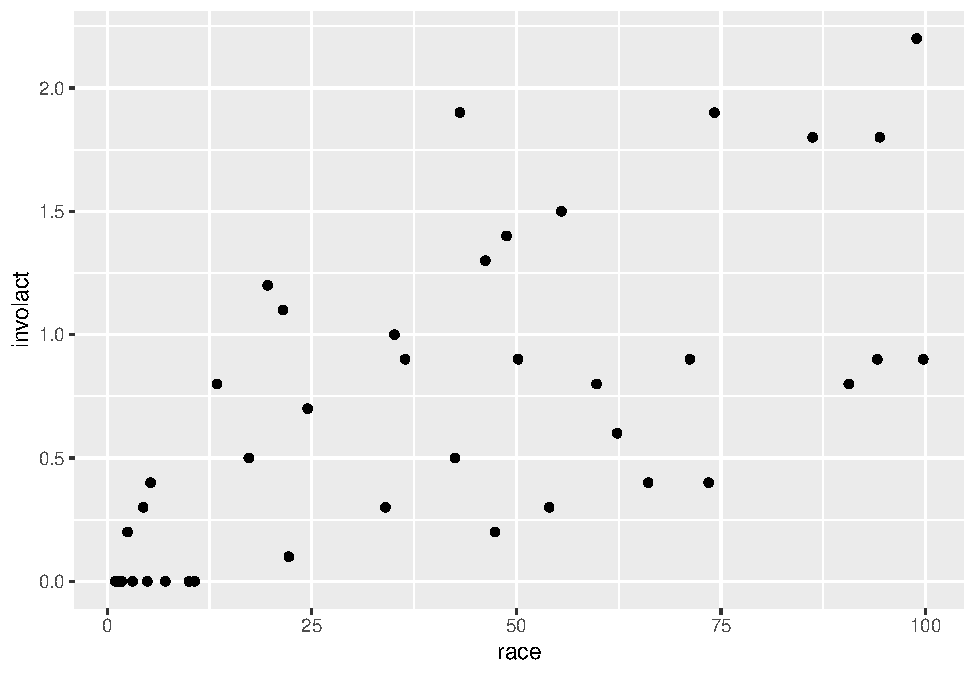
\includegraphics{intro_stats_files/figure-latex/unnamed-chunk-177-1.pdf}

\hypertarget{exercise-1-4}{%
\paragraph*{Exercise 1}\label{exercise-1-4}}
\addcontentsline{toc}{paragraph}{Exercise 1}

Does the Chicago redlining data come from an observational study or an experiment? How do you know?

Please write up your answer here.

\begin{center}\rule{0.5\linewidth}{0.5pt}\end{center}

If certain conditions are met, we can graph a regression line; just add a \texttt{geom\_smooth} layer to the scatterplot:

\begin{Shaded}
\begin{Highlighting}[]
\FunctionTok{ggplot}\NormalTok{(chredlin, }\FunctionTok{aes}\NormalTok{(}\AttributeTok{y =}\NormalTok{ involact, }\AttributeTok{x =}\NormalTok{ race)) }\SpecialCharTok{+}
    \FunctionTok{geom\_point}\NormalTok{() }\SpecialCharTok{+}
    \FunctionTok{geom\_smooth}\NormalTok{(}\AttributeTok{method =}\NormalTok{ lm, }\AttributeTok{se =} \ConstantTok{FALSE}\NormalTok{)}
\end{Highlighting}
\end{Shaded}

\begin{verbatim}
## `geom_smooth()` using formula 'y ~ x'
\end{verbatim}

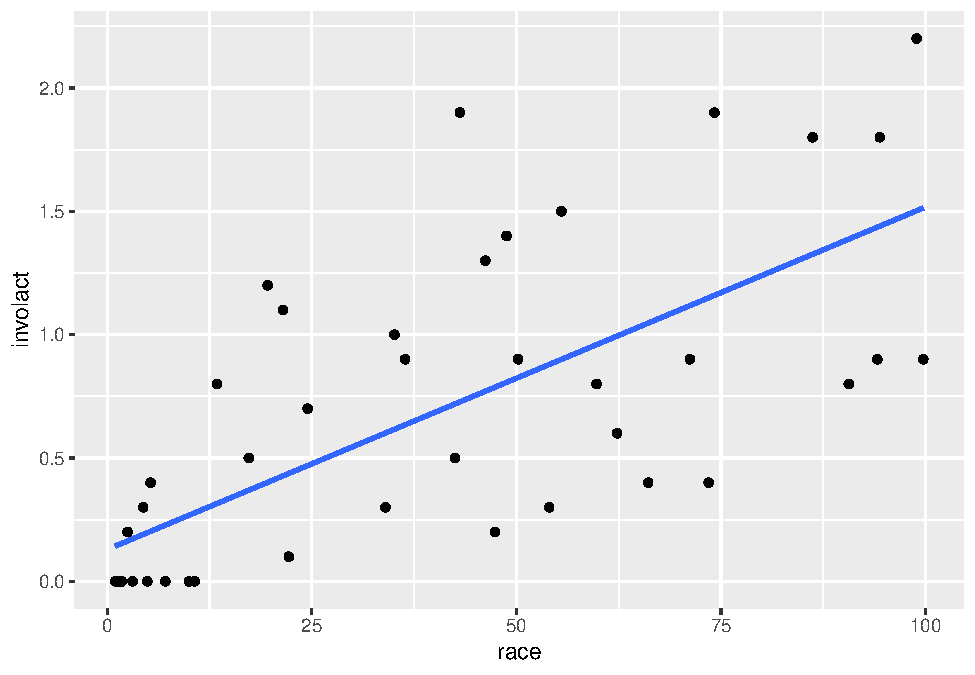
\includegraphics{intro_stats_files/figure-latex/unnamed-chunk-178-1.pdf}

The \texttt{method\ =\ lm} argument is telling \texttt{ggplot} to use a ``linear model''. The \texttt{se\ =\ FALSE} argument tells \texttt{ggplot} to draw just the line and nothing else. (What else might it try to draw? You are encouraged to go back to the code above and take out \texttt{se\ =\ FALSE} to see for yourself. However, we are not yet in a position to be able to explain the gray band that appears. We will return to this mystery in a future chapter.)

Of all possible lines, the blue line comes the closest to each point in the scatterplot. If we wiggled the line a little bit, it might get closer to a few points, but the net effect would be to make it further from other points. This is the mathematically optimal line of best fit.

\hypertarget{regression-models}{%
\section{Models}\label{regression-models}}

We used the word ``model'' when referring to the regression line above. What does that word mean in this context?

A model is something that represents something else, often on a smaller scale or in simplified form. A model is often an idealized form of something that may be quite messy or complex in reality. In statistics, a model is a representation of the way data is generated. For example, we may believe that as minority representation increases in a neighborhood, that neighborhood is more likely to be subject to racially discriminatory practices. We may even posit that the relationship is linear; i.e., for every percentage point increase in racial minorities, we expect some kind of proportional increase in racial discrimination, as measured in this case by FAIR policies. We say that this is our hypothesis about the \emph{data-generating process}: we suspect that the data we see results from a sociological process that uses the minority representation of a neighborhood to generate data about FAIR policies.

The assumption of a linear relationship between these two quantities is just that---an assumption. It is not necessarily ``true'', whatever ``true'' might mean in this kind of question. It is a convenient device that makes a simplifying assumption in order to allow us to do something meaningful in a statistical analysis. If such a model---despite its simplifying caricature---helps us make meaningful predictions to study something important like racial discrimination, then the model is useful.

The first thing we acknowledge when working with a model is that the model does not generate the data in a rigid, deterministic way. If you look at the scatterplot above, even assuming the blue line represents a ``correct'' data-generating process, the data points don't fall on the blue line. The blue line gives us only a sense of where the data might be, but there is additional space between the line and the points. These spaces are often referred to as \emph{errors}. In statistics, the word ``error'' does not mean the same thing as ``mistake''. Error is just the difference between an idealized model prediction and the real location of data. In the context of linear regression, we will use the term \emph{residual} instead. After the model is done making a prediction, the residuals are ``left over'' to account for the different between the model and the actual data.

The most important thing to remember about models is that they aren't real. They are idealizations and simplifications. The degree to which we can trust models, then, comes down to certain assumptions we make about the data-generating process. These assumptions cannot be completely verified---after all, we will never know the exact data-generating process. But there are certain \emph{conditions} we can check to know if the assumptions we make are reasonable.

\hypertarget{exercise-2-3}{%
\paragraph*{Exercise 2}\label{exercise-2-3}}
\addcontentsline{toc}{paragraph}{Exercise 2}

Do an internet search for the phrase ``statistical model'' and/or ``statistical modeling''. Read at least two or three sources. List below one important aspect of statistical modeling you find in your search that wasn't mentioned in the paragraphs above. (Some of the sources you find may be a little technical. You should, for now, skip over the technical explanations. Try to find several sources that address the issue in non-technical ways. The additional information you mention below should be something non-technical that you understand.)

Please write up your answer here.

\begin{center}\rule{0.5\linewidth}{0.5pt}\end{center}

\hypertarget{regression-conditions}{%
\section{Checking conditions}\label{regression-conditions}}

We need to be careful here. Although we graphed the blue regression line above, we have not checked any conditions. Therefore, it is inappropriate to fit a regression line at this point. Once the line is seen, it cannot easily be ``unseen'', and it's crucial that you don't trick your eyes into believing there is a linear relationship before checking the conditions that justify that belief.

The regression line we saw above makes no sense unless we know that regression is appropriate. The conditions for running a regression analysis include all the conditions you checked for a correlation analysis in the last chapter:

\begin{enumerate}
\def\labelenumi{\arabic{enumi}.}
\tightlist
\item
  The two variables must be numerical.
\item
  There is a somewhat linear relationship between the variables, as shown in a scatterplot.
\item
  There are no serious outliers.
\end{enumerate}

\hypertarget{exercise-3-3}{%
\paragraph*{Exercise 3}\label{exercise-3-3}}
\addcontentsline{toc}{paragraph}{Exercise 3}

Check these three conditions for the regression between \texttt{involact} and \texttt{race} (using the scatterplot above for conditions (2) and (3).)

\begin{enumerate}
\def\labelenumi{\arabic{enumi}.}
\tightlist
\item
\item
\item
\end{enumerate}

\begin{center}\rule{0.5\linewidth}{0.5pt}\end{center}

However, there is an additional condition to check to ensure that our regression model is appropriate. It concerns the residuals, but as we haven't computed anything yet, we have nothing to analyze. We'll return to this condition later.

\hypertarget{regression-calculating}{%
\section{Calculating the regression line}\label{regression-calculating}}

What is the equation of the regression line? In your algebra class you learned that a line takes the form \(y = mx + b\) where \(m\) is the slope and \(b\) is the y-intercept. Statisticians write the equation in a slightly different form:

\[
\hat{y} = b_{0} + b_{1} x
\]

The intercept is \(b_{0}\) and the slope is \(b_{1}\). We use \(\hat{y}\) (pronounced ``y hat'') instead of \(y\) because when we plug in values of \(x\), we do not get back the exact values of \(y\) from the data. The line, after all, does not actually pass through most (if any) actual data points. Instead, this equation gives us ``predicted'' values of \(y\) that lie on the regression line. These predicted \(y\) values are called \(\hat{y}\).

To run a regression analysis and calculate the values of the intercept and slope, we use the \texttt{lm} command in R. (Again, \texttt{lm} stands for ``linear model''.) This command requires us to specify a ``formula'' that tells R the relationship we want to model. It uses special syntax in a very specific order:

\begin{itemize}
\tightlist
\item
  The response variable,
\item
  a ``tilde'' \textasciitilde{} (this key is usually in the upper-left corner of your keyboard, above the backtick),
\item
  the predictor variable.
\end{itemize}

After a comma, we then specify the data set in which those variables live using \texttt{data\ =}. Here's the whole command:

\begin{Shaded}
\begin{Highlighting}[]
\FunctionTok{lm}\NormalTok{(involact }\SpecialCharTok{\textasciitilde{}}\NormalTok{ race, }\AttributeTok{data =}\NormalTok{ chredlin)}
\end{Highlighting}
\end{Shaded}

\begin{verbatim}
## 
## Call:
## lm(formula = involact ~ race, data = chredlin)
## 
## Coefficients:
## (Intercept)         race  
##     0.12922      0.01388
\end{verbatim}

\textbf{The response variable always goes before the tilde and the predictor variable always goes after.}

Let's store that result for future use. The convention we'll use in this book is to name things using the variables involved. For example,

\begin{Shaded}
\begin{Highlighting}[]
\NormalTok{involact\_race\_lm }\OtherTok{\textless{}{-}} \FunctionTok{lm}\NormalTok{(involact }\SpecialCharTok{\textasciitilde{}}\NormalTok{ race, }\AttributeTok{data =}\NormalTok{ chredlin)}
\NormalTok{involact\_race\_lm}
\end{Highlighting}
\end{Shaded}

\begin{verbatim}
## 
## Call:
## lm(formula = involact ~ race, data = chredlin)
## 
## Coefficients:
## (Intercept)         race  
##     0.12922      0.01388
\end{verbatim}

The variable \texttt{involact\_race\_lm} now contains all the information we need about the linear regression model.

\hypertarget{regression-interpreting}{%
\section{Interpreting the coefficients}\label{regression-interpreting}}

Look at the output of the \texttt{lm} command above.

The intercept is 0.12922 and the slope is 0.01388. The number 0.12922 is labeled with \texttt{(Intercept)}, so that's pretty obvious. But how do we know the number 0.01388 corresponds to the slope? Process of elimination, I suppose. But there's another good reason too. The equation of the regression line can be written

\[
\hat{y} = 0.12922 + 0.01388 x
\]

When we report the equation of the regression line, we typically use words instead of \(\hat{y}\) and \(x\) to make the equation more interpretable in the context of the problem. For example, for this data, we would write the equation as

\[
\widehat{involact} = 0.12922 + 0.01388 race
\]

The slope is the \emph{coefficient} of \texttt{race}, or the number attached to \texttt{race}. (The intercept is not attached to anything; it's just a constant term out front there.)

The slope \(b_{1}\) is always interpretable. This model predicts that one unit of increase in the x-direction corresponds to a change of 0.01388 units in the y-direction. Let's phrase it this way:

\begin{quote}
The model predicts that an increase of one percentage point in the composition of racial minorities corresponds to an increase of 0.01388 new FAIR policies per 100 housing units.
\end{quote}

The intercept \(b_{0}\) is a different story. There is always a literal interpretation:

\begin{quote}
The model predicts that a ZIP code with 0\% racial minorites will generate 0.12922 new FAIR policies.
\end{quote}

In some cases (rarely), that interpretation might make sense. In most cases, though, it is physically impossible for the predictor variable to take a value of 0, or the value 0 is way outside the range of the data. Whenever we use a model to make a prediction outside of reasonable values, we call that \emph{extrapolation}.

For the Chicago data, we likely don't have a case of extrapolation. While it is not literally true that any ZIP code has 0\% racial minorities, we can see in the scatterplot that there are values very close to zero.

\hypertarget{exercise-4-3}{%
\paragraph*{Exercise 4}\label{exercise-4-3}}
\addcontentsline{toc}{paragraph}{Exercise 4}

Use the \texttt{arrange} command from \texttt{dplyr} to sort the \texttt{chredlin} data frame by race (using the default ascending order). What is the value of \texttt{race} for the three ZIP codes with the smallest percentage of minority residents?

\begin{Shaded}
\begin{Highlighting}[]
\CommentTok{\# Add code here to sort by race}
\end{Highlighting}
\end{Shaded}

Please write up your answer here.

\begin{center}\rule{0.5\linewidth}{0.5pt}\end{center}

Again, even though there are no ZIP codes with 0\% racial minorities, there are a bunch that are close to zero, so the literal interpretation of the intercept is also likely a sensible one in this case.

\hypertarget{exercise-5-3}{%
\paragraph*{Exercise 5}\label{exercise-5-3}}
\addcontentsline{toc}{paragraph}{Exercise 5}

Let's think through something else the intercept might be telling us in this case. The presumption is that FAIR policies are obtained mostly by folks who can't get insurance policies in other ways. Some of that is driven by racial discrimination, but maybe not all of it. What does the intercept have to say about the number of FAIR policies that are obtained \emph{not} due to denial of coverage from racial discrimination?

Please write up your answer here.

\hypertarget{regression-rescaling}{%
\section{Rescaling to make interpretations more meaningful}\label{regression-rescaling}}

Let's revisit the interpretation of the slope:

\begin{quote}
The model predicts that an increase of one percentage point in the composition of racial minorities corresponds to an increase of 0.01388 new FAIR policies per 100 housing units.
\end{quote}

This is a perfectly correct statement, but one percentage point change is not very much. It's hard to think about comparing two neighborhoods that differ by only one percent. This scale also makes the predicted change in the response variable hard to interpret. How many policies is 0.01388 per 100 housing units?

One way to make these kinds of statements more interpretable is to change the scale. What if we increase 10 percentage points instead of only 1 percentage point? In other words, what if we move 10 times as far along the x-axis. The response variable will also have to move 10 times as far. This is the new statement:

\begin{quote}
The model predicts that an increase of 10 percentage points in the composition of racial minorities corresponds to an increase of 0.1388 new FAIR policies per 100 housing units.
\end{quote}

In this case, the decimal 0.1388 is maybe still not completely clear, but at least an increase of 10 percentage points is a meaningful difference between neighborhoods.

\hypertarget{exercise-6-2}{%
\paragraph*{Exercise 6}\label{exercise-6-2}}
\addcontentsline{toc}{paragraph}{Exercise 6}

Since the last number is a \emph{per capita} type measure, we can also rescale it. If the model predicts an increase in 0.1388 new FAIR policies per 100 households (corresponding to 10 percentage points increase in racial minorities), how many FAIR policies would that be in 1000 households?

Please write up your answer here.

\hypertarget{regression-tidy}{%
\section{\texorpdfstring{The \texttt{tidy} command}{The tidy command}}\label{regression-tidy}}

Recall the output of the \texttt{lm} command:

\begin{Shaded}
\begin{Highlighting}[]
\NormalTok{involact\_race\_lm}
\end{Highlighting}
\end{Shaded}

\begin{verbatim}
## 
## Call:
## lm(formula = involact ~ race, data = chredlin)
## 
## Coefficients:
## (Intercept)         race  
##     0.12922      0.01388
\end{verbatim}

(We did not have to run \texttt{lm} again. We had this output stored in the variable \texttt{involact\_race\_lm}.)

That summary is fine, but what if we needed to reference the slope and intercept using inline code? Or what if we wanted to grab those numbers and use them in further calculations?

The problem is that the results of \texttt{lm} just print the output in an unstructured way. If we want structured input, we can use the \texttt{tidy} command from the \texttt{broom} package. This will take the results of \texttt{lm} and organize the output into a tibble.

\begin{Shaded}
\begin{Highlighting}[]
\FunctionTok{tidy}\NormalTok{(involact\_race\_lm)}
\end{Highlighting}
\end{Shaded}

\begin{verbatim}
## # A tibble: 2 x 5
##   term        estimate std.error statistic      p.value
##   <chr>          <dbl>     <dbl>     <dbl>        <dbl>
## 1 (Intercept)   0.129    0.0966       1.34 0.188       
## 2 race          0.0139   0.00203      6.84 0.0000000178
\end{verbatim}

Let's store that tibble so we can refer to it in the future.

\begin{Shaded}
\begin{Highlighting}[]
\NormalTok{involact\_race\_tidy }\OtherTok{\textless{}{-}} \FunctionTok{tidy}\NormalTok{(involact\_race\_lm)}
\NormalTok{involact\_race\_tidy}
\end{Highlighting}
\end{Shaded}

\begin{verbatim}
## # A tibble: 2 x 5
##   term        estimate std.error statistic      p.value
##   <chr>          <dbl>     <dbl>     <dbl>        <dbl>
## 1 (Intercept)   0.129    0.0966       1.34 0.188       
## 2 race          0.0139   0.00203      6.84 0.0000000178
\end{verbatim}

The intercept is stored in the \texttt{estimate} column, in the first row. The slope is stored in the same column, but in the second row. (There is a lot more information here to the right of the \texttt{estimate} column, but we will not know what these numbers mean until later in the course.)

We can grab the \texttt{estimate} column with the dollar sign as we've seen before:

\begin{Shaded}
\begin{Highlighting}[]
\NormalTok{involact\_race\_tidy}\SpecialCharTok{$}\NormalTok{estimate}
\end{Highlighting}
\end{Shaded}

\begin{verbatim}
## [1] 0.12921803 0.01388235
\end{verbatim}

This is a ``vector'' of two values, the intercept and the slope, respectively.

What if we want only one value at a time? We can grab individual elements of a vector using square brackets as follows:

\begin{Shaded}
\begin{Highlighting}[]
\NormalTok{involact\_race\_tidy}\SpecialCharTok{$}\NormalTok{estimate[}\DecValTok{1}\NormalTok{]}
\end{Highlighting}
\end{Shaded}

\begin{verbatim}
## [1] 0.129218
\end{verbatim}

\begin{Shaded}
\begin{Highlighting}[]
\NormalTok{involact\_race\_tidy}\SpecialCharTok{$}\NormalTok{estimate[}\DecValTok{2}\NormalTok{]}
\end{Highlighting}
\end{Shaded}

\begin{verbatim}
## [1] 0.01388235
\end{verbatim}

Here is the interpretation of the slope again, but this time, we'll use inline code:

\begin{quote}
The model predicts that an increase of 1 percentage points in the composition of racial minorities corresponds to an increase of 0.0138824 new FAIR policies per 100 housing units.
\end{quote}

Click somewhere inside the backticks on the line above and hit Ctrl-Enter or Cmd-Enter (PC or Mac respectively). You should see the number 0.01388235 pop up. If you Preview the HTML version of the document, you will also see the number there (not the code).

What if we want to apply re-scaling to make this number more interpretable? The stuff inside the inline code chunk is just R code, so we can do any kind of calculation with it we want.

\begin{quote}
The model predicts that an increase of 10 percentage points in the composition of racial minorities corresponds to an increase of 0.1388235 new FAIR policies per 100 housing units.
\end{quote}

Now the number will be 0.1388235, ten times as large.

\hypertarget{exercise-7-1}{%
\paragraph*{Exercise 7}\label{exercise-7-1}}
\addcontentsline{toc}{paragraph}{Exercise 7}

Copy and paste the interpretation of the intercept from earlier, but replace the number 0.12922 with an inline code chunk that grabs that number from the \texttt{estimate} column of the \texttt{involact\_race\_tidy} tibble. (Remember that the intercept is the \emph{first} element of that vector, not the second element like the slope.)

Please write up your answer here.

\hypertarget{regression-residuals}{%
\section{Residuals}\label{regression-residuals}}

Earlier, we promised to revisit the topic of residuals. Residuals are measured as the vertical distances from each data point to the regression line. We can see that visually below. (Don't worry about the complexity of the \texttt{ggplot} code used to create this picture. You will not need to create a plot like this on your own, so just focus on the graph that is created below.)

\begin{Shaded}
\begin{Highlighting}[]
\FunctionTok{ggplot}\NormalTok{(chredlin, }\FunctionTok{aes}\NormalTok{(}\AttributeTok{y =}\NormalTok{ involact, }\AttributeTok{x =}\NormalTok{ race)) }\SpecialCharTok{+}
    \FunctionTok{geom\_segment}\NormalTok{(}\AttributeTok{x =} \FloatTok{35.1}\NormalTok{, }\AttributeTok{xend  =} \FloatTok{35.1}\NormalTok{,}
                 \AttributeTok{y =} \FloatTok{0.6164886}\NormalTok{, }\AttributeTok{yend =} \FloatTok{0.6164886} \SpecialCharTok{+} \FloatTok{0.38351139}\NormalTok{,}
                 \AttributeTok{color =} \StringTok{"red"}\NormalTok{, }\AttributeTok{size =} \DecValTok{2}\NormalTok{) }\SpecialCharTok{+}
    \FunctionTok{geom\_segment}\NormalTok{(}\AttributeTok{x =} \FloatTok{66.1}\NormalTok{, }\AttributeTok{xend =} \FloatTok{66.1}\NormalTok{,}
                 \AttributeTok{y =} \FloatTok{1.0468415}\NormalTok{, }\AttributeTok{yend =} \FloatTok{1.0468415} \SpecialCharTok{{-}} \FloatTok{0.64684154}\NormalTok{,}
                 \AttributeTok{color =} \StringTok{"red"}\NormalTok{, }\AttributeTok{size =} \DecValTok{2}\NormalTok{) }\SpecialCharTok{+}
    \FunctionTok{geom\_point}\NormalTok{() }\SpecialCharTok{+}
    \FunctionTok{geom\_smooth}\NormalTok{(}\AttributeTok{method =}\NormalTok{ lm, }\AttributeTok{se =} \ConstantTok{FALSE}\NormalTok{)}
\end{Highlighting}
\end{Shaded}

\begin{verbatim}
## `geom_smooth()` using formula 'y ~ x'
\end{verbatim}

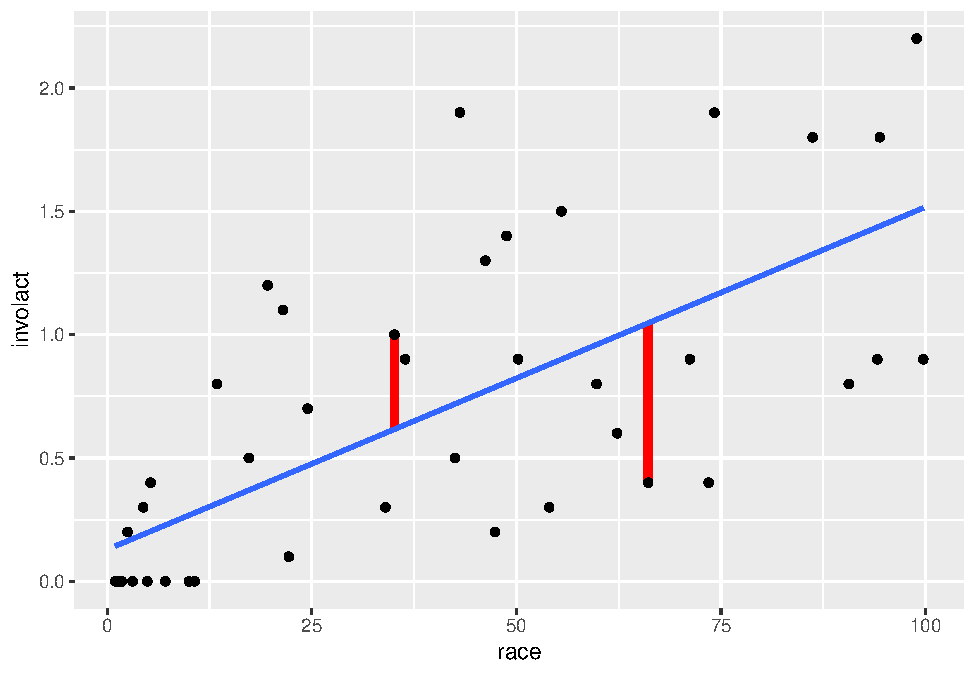
\includegraphics{intro_stats_files/figure-latex/unnamed-chunk-188-1.pdf}

The graph above shows the regression line and two of the residuals as red line segments. (There is a residual for all 47 ZIP codes; only two are shown in this graph.) The one on the left corresponds to ZIP code with 35\% racial minority. The regression line predicts that, if the model were true, such a ZIP code would have a value of \texttt{involact} of about 0.6. But the actual data for that ZIP code has an \texttt{involact} value of 1. The residual is the difference, about 0.4. In other words, the true data point is 0.4 units higher than the model prediction. This represents a \emph{positive} residual; the actual data is 0.4 units \emph{above} the line. Data points that lie below the regression line have \emph{negative} residuals.

\hypertarget{exercise-8-2}{%
\paragraph*{Exercise 8}\label{exercise-8-2}}
\addcontentsline{toc}{paragraph}{Exercise 8}

Look at the residual on the right. This corresponds to a ZIP code with about 66\% racial minorities. First, estimate the value of \texttt{involact} that the model predicts for this ZIP code. (This is the y-value of the point on the regression line.) Next, report the actual \texttt{involact} value for this ZIP code. Finally, subtract these two numbers to get an approximate value for the residual. Should this residual be a positive number or a negative number?

You can just estimate with your eyeballs for now. You don't need to be super precise.

Please write up your answer here.

\begin{center}\rule{0.5\linewidth}{0.5pt}\end{center}

More formally, let's call the residual \(e\). This is standard notation, as ``e'' stands for ``error''. Again, though, it's not an error in the sense of a mistake. It's an error in the sense that the model is not perfectly accurate, so it doesn't predict the data points exactly. The degree to which the prediction misses is the ``error'' or ``residual''. It is given by the following formula:

\[
e = y - \hat{y}
\]

\hypertarget{exercise-9-1}{%
\paragraph*{Exercise 9}\label{exercise-9-1}}
\addcontentsline{toc}{paragraph}{Exercise 9}

There are two symbols on the right-hand side of the equation above, \(y\) and \(\hat{y}\). Which one is the actual data value and which one is the predicted value (the one on the line)?

Please write up your answer here.

\begin{center}\rule{0.5\linewidth}{0.5pt}\end{center}

The residuals are used to determine the regression line. The correct regression line will be the one that results in the smallest residuals overall. How do we measure the overall set of residuals? We can't just calculate the average residual. Because the regression line should go through the middle of the data, the positive residuals will cancel out the negative residuals and the mean residual will just be zero. That's not very useful.

Instead, what we do is \emph{square} the residuals. That makes all of them positive. Then we add together all the squared residuals and that sum is the thing we try to minimize. Well, we don't do that manually because it's hard, so we let the computer do that for us. Because the regression line minimizes the sum of the squared residuals, the regression line is often called the \emph{least-squares} line.

Recall earlier when we mentioned that there was one additional condition to check in order for linear regression to make sense. This condition is that \textbf{there should not be any kind of pattern in the residuals}.

We know that some of the points are going to lie above the line (positive residuals) and some of the points will lie below the line (negative residuals). What we need is for the spread of the residuals to be pretty balanced across the length of the regression line and for the residuals not to form any kind of curved pattern.

To check this condition, we'll need to calculate the residuals first. To do so, we introduce a new function from the \texttt{broom} package. Whereas \texttt{tidy} serves up information about the intercept and the slope of the regression line, \texttt{augment} gives us extra information for each data point.

\begin{Shaded}
\begin{Highlighting}[]
\NormalTok{involact\_race\_aug }\OtherTok{\textless{}{-}} \FunctionTok{augment}\NormalTok{(involact\_race\_lm)}
\NormalTok{involact\_race\_aug}
\end{Highlighting}
\end{Shaded}

\begin{verbatim}
## # A tibble: 47 x 9
##    .rownames involact  race .fitted .resid   .hat .sigma .cooksd .std.resid
##    <chr>        <dbl> <dbl>   <dbl>  <dbl>  <dbl>  <dbl>   <dbl>      <dbl>
##  1 60626          0    10     0.268 -0.268 0.0341  0.452 0.00651     -0.608
##  2 60640          0.1  22.2   0.437 -0.337 0.0246  0.451 0.00731     -0.761
##  3 60613          1.2  19.6   0.401  0.799 0.0261  0.437 0.0436       1.80 
##  4 60657          0.5  17.3   0.369  0.131 0.0277  0.453 0.00124      0.295
##  5 60614          0.7  24.5   0.469  0.231 0.0235  0.453 0.00326      0.520
##  6 60610          0.3  54     0.879 -0.579 0.0287  0.445 0.0253      -1.31 
##  7 60611          0     4.9   0.197 -0.197 0.0398  0.453 0.00417     -0.448
##  8 60625          0     7.1   0.228 -0.228 0.0372  0.453 0.00517     -0.517
##  9 60618          0.4   5.3   0.203  0.197 0.0393  0.453 0.00411      0.448
## 10 60647          1.1  21.5   0.428  0.672 0.0250  0.442 0.0295       1.52 
## # ... with 37 more rows
\end{verbatim}

The first three columns consist of the row names (the ZIP codes) followed by the actual data values we started with for \texttt{involact} and \texttt{race}. But now we've ``augmented'' the original data with some new stuff too. (We won't learn about anything past the fifth column in this course, though.)

The fourth column---called \texttt{.fitted}---is \(\hat{y}\), or the point on the line that corresponds to the given \(x\) value. Let's check and make sure this is working as advertised.

The regression equation from above is

\[
\widehat{involact} = 0.12922 + 0.01388 race
\]

Take, for example, the first row in the tibble above, the one corresponding to ZIP code 60626. The value of \texttt{race} is 10.0. Plug that value into the equation above:

\[
\widehat{involact} = 0.12922 + 0.01388(10.0) = 0.268
\]

The model predicts that a ZIP code with 10\% racial minorities will have about 0.268 new FAIR policies per 100 housing units. The corresponding number in the \texttt{.fitted} column is 0.2680416, so that's correct.

Now skip over to the fifth column of the \texttt{augment} output, the one that says \texttt{.resid}. If this is the residual \(e\), then it should be \(y - \hat{y}\). Since \(y\) is the actual value of \texttt{involact} and \(\hat{y}\) is the value predicted by the model, we should get for the first row of output

\[
e = y - \hat{y} = 0.0 - 0.268 = -0.268
\]

Yup, it works!

To check for patterns in the residuals, we'll create a \emph{residual plot}. A residual plot graphs the residuals above each value along the x-axis. (In the command below, we also add a blue horizontal reference line so that it is clear which points have positive or negative residuals.)

\begin{Shaded}
\begin{Highlighting}[]
\FunctionTok{ggplot}\NormalTok{(involact\_race\_aug, }\FunctionTok{aes}\NormalTok{(}\AttributeTok{y =}\NormalTok{ .resid, }\AttributeTok{x =}\NormalTok{ race)) }\SpecialCharTok{+}
    \FunctionTok{geom\_point}\NormalTok{() }\SpecialCharTok{+}
    \FunctionTok{geom\_hline}\NormalTok{(}\AttributeTok{yintercept =} \DecValTok{0}\NormalTok{, }\AttributeTok{color =} \StringTok{"blue"}\NormalTok{)}
\end{Highlighting}
\end{Shaded}

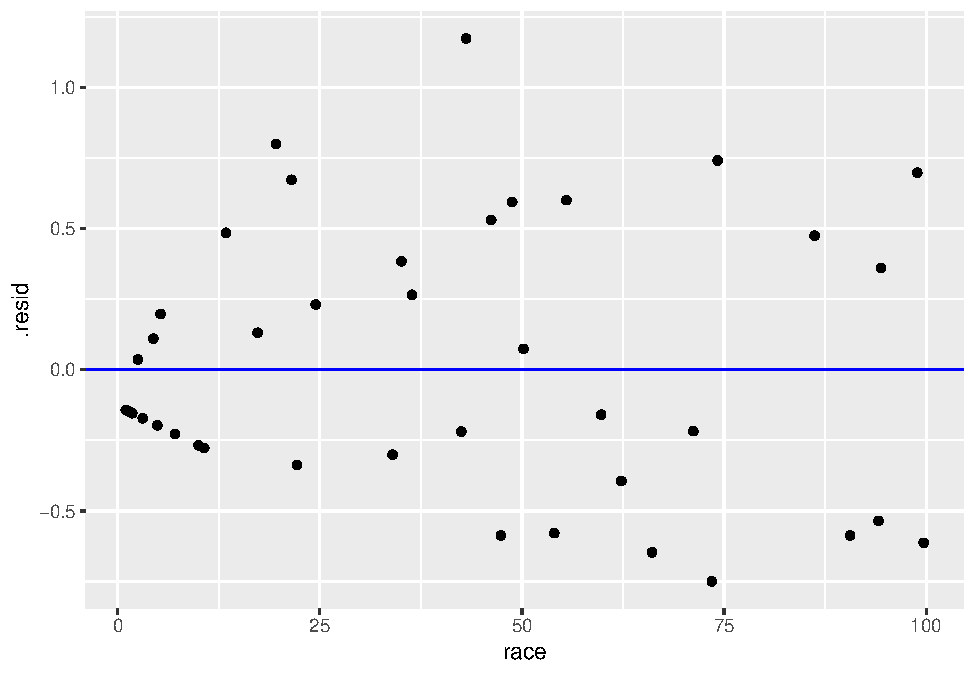
\includegraphics{intro_stats_files/figure-latex/unnamed-chunk-190-1.pdf}

Pay close attention to the \texttt{ggplot} code. Notice that the tibble in the first slot is \emph{not} \texttt{chredlin} as it was before. The residuals we need to plot are not stored in the raw \texttt{chredlin} data. We had to calculate the residuals using the \texttt{augment} command, and those residuals are then stored in a different place that we named \texttt{involact\_race\_aug}. In the latter tibble, the residuals themselves are stored in a variable called \texttt{.resid}. (Don't forget the dot in \texttt{.resid}.)

We are looking for systematic patterns in the residuals. A good residual plot should look like the most boring plot you've ever seen.

For the most part, the residual plot above looks pretty good. The one exception is the clustering near the left edge of the graph.

\hypertarget{exercise-10-3}{%
\paragraph*{Exercise 10}\label{exercise-10-3}}
\addcontentsline{toc}{paragraph}{Exercise 10}

Refer back and forth between the original scatterplot created earlier (with the regression line) and the residual plot above. Can you explain why there is a line of data points with negative residuals along the left edge of the residual plot?

Please write up your answer here.

\begin{center}\rule{0.5\linewidth}{0.5pt}\end{center}

Residual patterns that are problematic often involve curved data (where the dots follow a curve around the horizontal reference line instead of spreading evenly around it) and \emph{heteroscedasticity}, which is a fanning out pattern from left to right.

Other than the weird cluster of points at the left, the rest of the residual plot looks pretty good. Ignoring those ZIP codes with 0 FAIR policies, the rest of the residuals stretch, on average, about the same height above and below the line across the whole width of the plot. There is only one slightly large residual at about the 40\% mark, but it's not extreme, and it doesn't look like a severe outlier in the original scatterplot.

What does a bad residual plot look like? The code below will run an ill-advised regression analysis on \texttt{fire}, the number of fires (per 100 housing units), against \texttt{age}, the percent of housing units built before 1939. The residual plot appears below.

\begin{Shaded}
\begin{Highlighting}[]
\NormalTok{fire\_age\_lm }\OtherTok{\textless{}{-}} \FunctionTok{lm}\NormalTok{(fire }\SpecialCharTok{\textasciitilde{}}\NormalTok{ age, }\AttributeTok{data =}\NormalTok{ chredlin)}
\NormalTok{fire\_age\_aug }\OtherTok{\textless{}{-}} \FunctionTok{augment}\NormalTok{(fire\_age\_lm)}
\FunctionTok{ggplot}\NormalTok{(fire\_age\_aug, }\FunctionTok{aes}\NormalTok{(}\AttributeTok{y =}\NormalTok{ .resid, }\AttributeTok{x =}\NormalTok{ age)) }\SpecialCharTok{+}
    \FunctionTok{geom\_point}\NormalTok{() }\SpecialCharTok{+}
    \FunctionTok{geom\_hline}\NormalTok{(}\AttributeTok{yintercept =} \DecValTok{0}\NormalTok{, }\AttributeTok{color =} \StringTok{"blue"}\NormalTok{)}
\end{Highlighting}
\end{Shaded}

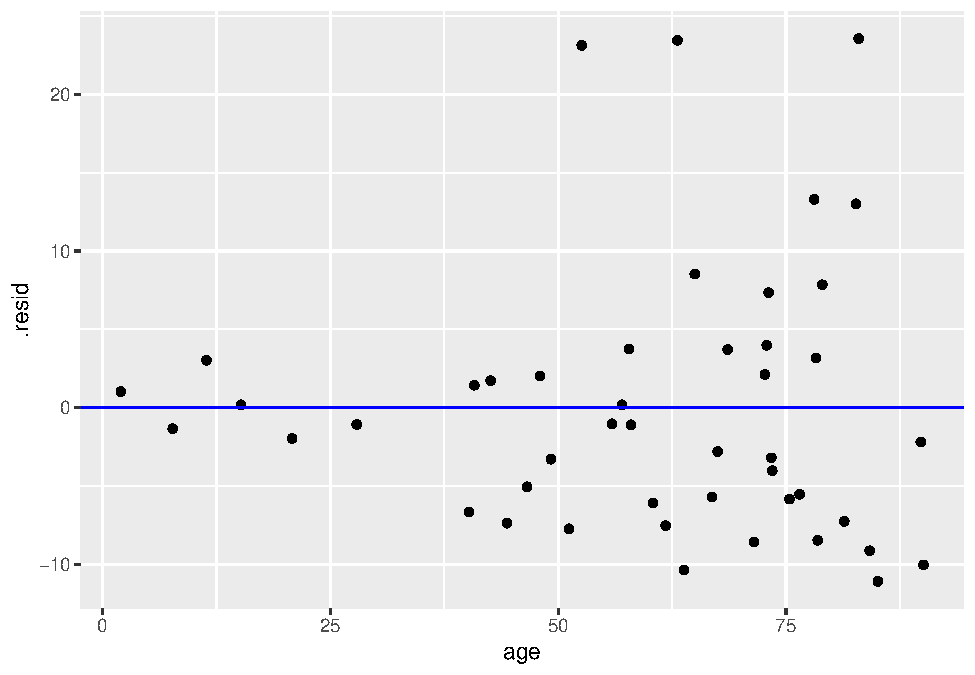
\includegraphics{intro_stats_files/figure-latex/unnamed-chunk-191-1.pdf}

\hypertarget{exercise-11-3}{%
\paragraph*{Exercise 11}\label{exercise-11-3}}
\addcontentsline{toc}{paragraph}{Exercise 11}

Using the vocabulary established above, explain why the residual plot above is bad.

Please write up your answer here.

\begin{center}\rule{0.5\linewidth}{0.5pt}\end{center}

Of course, we should never even get as far as running a regression analysis and making a residual plot if we perform exploratory data analysis as we're supposed to.

\hypertarget{exercise-12a}{%
\paragraph*{Exercise 12(a)}\label{exercise-12a}}
\addcontentsline{toc}{paragraph}{Exercise 12(a)}

If you were truly interested in investigating an association between the fire risk and the age of buildings in a ZIP code, the first thing you would do is create a scatterplot. Go ahead and do that below. Use \texttt{fire} as the response variable and \texttt{age} as the predictor.

\begin{Shaded}
\begin{Highlighting}[]
\CommentTok{\# Add code here to create a scatterplot of fire against age}
\end{Highlighting}
\end{Shaded}

\hypertarget{exercise-12b}{%
\paragraph*{Exercise 12(b)}\label{exercise-12b}}
\addcontentsline{toc}{paragraph}{Exercise 12(b)}

From the scatterplot above, explain why you wouldn't even get as far as running a regression analysis. (Think of the conditions.)

Please write up your answer here.

\begin{center}\rule{0.5\linewidth}{0.5pt}\end{center}

To review, the conditions for a regression analysis are as follows (including the newest fourth condition):

\begin{enumerate}
\def\labelenumi{\arabic{enumi}.}
\tightlist
\item
  The two variables must be numerical.
\item
  There is a somewhat linear relationship between the variables, as shown in a scatterplot.
\item
  There are no serious outliers.
\item
  \textbf{There is no pattern in the residuals.}
\end{enumerate}

\hypertarget{regression-r2}{%
\section{\texorpdfstring{\(R^2\)}{R\^{}2}}\label{regression-r2}}

We've seen that the correlation coefficient r is of limited utility. In addition to being only a single statistic to summarize a linear association, the number doesn't have any kind of intrinsic meaning. It can only be judged by how close it is to 0 or 1 (or -1) in conjunction with a scatterplot to give you a sense of the strength of the correlation. \textbf{In particular, some people try to interpret r as some kind of percentage, but it's not.}

On the other hand, when we square the correlation coefficient, we \emph{do} get an interpretable number. For some reason, instead of writing \(r^2\), statisticians write \(R^2\), with a capital R. (I can't find the historical reason why this is so.) In any event, \(R^2\) can be interpreted as a percentage! It represents the percent of variation in the y variable that can be explained by variation in the x variable.

Here we introduce the last of the \texttt{broom} functions: \texttt{glance}. Whereas \texttt{tidy} reports the intercept and slope, and \texttt{augment} reports values associated to each data point separately, the \texttt{glance} function gathers up summaries for the entire model. (Do not confuse \texttt{glance} with \texttt{glimpse}. The latter is a nicer version of \texttt{str} that just summarizes the variables in a tibble.)

\begin{Shaded}
\begin{Highlighting}[]
\NormalTok{involact\_race\_glance }\OtherTok{\textless{}{-}} \FunctionTok{glance}\NormalTok{(involact\_race\_lm)}
\NormalTok{involact\_race\_glance}
\end{Highlighting}
\end{Shaded}

\begin{verbatim}
## # A tibble: 1 x 12
##   r.squared adj.r.squared sigma statistic      p.value    df logLik   AIC   BIC
##       <dbl>         <dbl> <dbl>     <dbl>        <dbl> <dbl>  <dbl> <dbl> <dbl>
## 1     0.509         0.499 0.449      46.7 0.0000000178     1  -28.0  62.0  67.6
## # ... with 3 more variables: deviance <dbl>, df.residual <int>, nobs <int>
\end{verbatim}

A more advanced statistics course might discuss the other model summaries present in the \texttt{glance} output. The \(R^{2}\) value is stored in the \texttt{r.squared} (inexplicably, now written with a lowercase r). Its value is 0.51. We will word it this way:

\begin{quote}
51\% of the variability in FAIR policies can be accounted for by variability in racial composition.
\end{quote}

Another way to think about this is to imagine all the factors that might go into the number of FAIR policies obtained in a ZIP code. That number varies across ZIP codes, with some ZIP codes having essentially 0 FAIR policies per 100 housing units, and others having quite a bit more, up to 2 or more per 100 housing units. What accounts for this discrepancy among ZIP codes? Is it the varying racial composition of those neighborhoods? To some degree, yes. We have seen that more racially diverse neighborhoods, on average, require more FAIR policies. But is race the only factor? Probably not. Income, for example, might play a role. People in low income neighborhoods may not be able to acquire traditional insurance due to its cost or their poor credit, etc. That also accounts for some of the variability among ZIP codes. Are there likely even more factors? Most assuredly. In fact, if 51\% of the variability in FAIR policies can be accounted for by variability in racial composition. then 49\% must be accounted for by other variables. These other variables may or may not be collected in our data, and we will never be able to determine all the factors that go into varying FAIR policy numbers.

\(R^2\) is a measure of the fit of the model. High values of \(R^2\) mean that the line predicts the data values closely, whereas lower values of \(R^2\) mean that there is still a lot of variability left in the residuals (again, due to other factors that are not measured in the model).

\hypertarget{exercise-13-2}{%
\paragraph*{Exercise 13}\label{exercise-13-2}}
\addcontentsline{toc}{paragraph}{Exercise 13}

Calculate the correlation coefficient r between \texttt{involact} and \texttt{race} using the \texttt{cor} command. (You might have to look back at the last chapter to remember the syntax.) Store that value as r.

In a separate code chunk, square that value using the command \texttt{r\^{}2}. Verify that the square of the correlation coefficient is the same as the \(R^2\) value reported in the \texttt{glance} output above.

\begin{Shaded}
\begin{Highlighting}[]
\CommentTok{\# Add code here to calculate the correlation coefficient}
\end{Highlighting}
\end{Shaded}

\begin{Shaded}
\begin{Highlighting}[]
\CommentTok{\# Add code here to square the correlation coefficient}
\end{Highlighting}
\end{Shaded}

\hypertarget{regression-multiple}{%
\section{Multiple predictors}\label{regression-multiple}}

The discussion of \(R^2\) above highlights the fact that a single predictor will rarely account for all or even most of the variability in a response variable. Is there a way to take other predictors into account?

The answer is yes, and the statistical technique involved is called multiple regression. Multiple regression is a deep subject, worthy of entire courses. Suffice it to say here that more advanced stats courses go into the ways in which multiple predictors can be included in a regression.

One easy thing we can do is incorporate a categorical variable into a graph and see if that categorical variable might play a role in the regression analysis. For example, there is a variance called \texttt{side} in \texttt{chredlin} that indicates whether the ZIP code is on the north side (n) or south side(s) of Chicago. As described in an earlier chapter, we can use color to distinguish between the ZIP codes.

\begin{Shaded}
\begin{Highlighting}[]
\FunctionTok{ggplot}\NormalTok{(chredlin, }\FunctionTok{aes}\NormalTok{(}\AttributeTok{y =}\NormalTok{ involact, }\AttributeTok{x =}\NormalTok{ race, }\AttributeTok{color =}\NormalTok{ side)) }\SpecialCharTok{+}
    \FunctionTok{geom\_point}\NormalTok{()}
\end{Highlighting}
\end{Shaded}

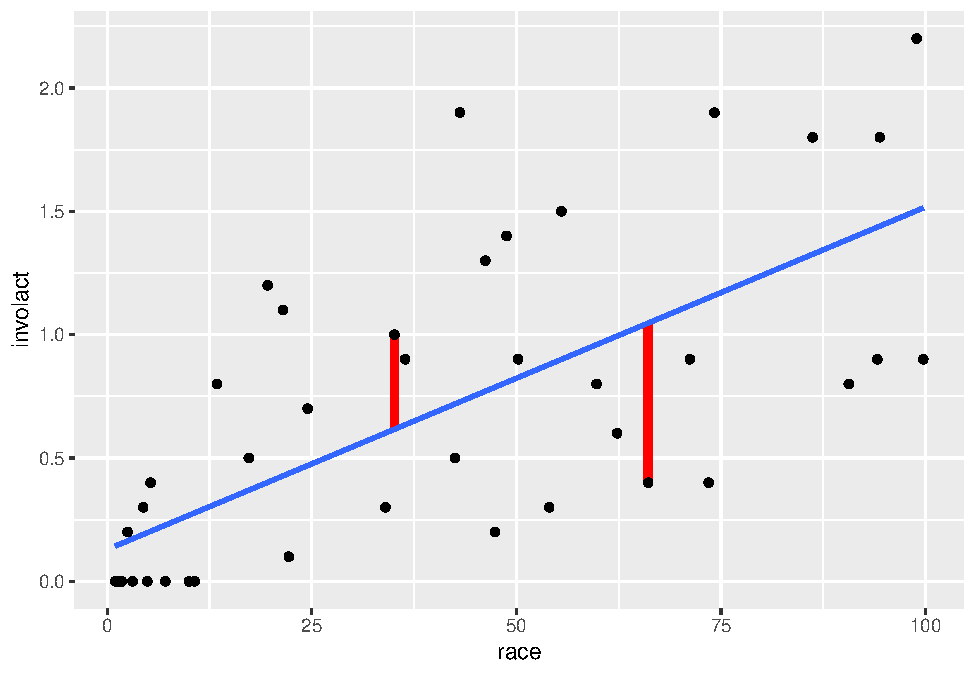
\includegraphics{intro_stats_files/figure-latex/unnamed-chunk-196-1.pdf}

\hypertarget{exercise-14}{%
\paragraph*{Exercise 14}\label{exercise-14}}
\addcontentsline{toc}{paragraph}{Exercise 14}

Do neighborhoods with higher percent racial minorities tend to be on the north or south side of Chicago?

Please write up your answer here.

\begin{center}\rule{0.5\linewidth}{0.5pt}\end{center}

Does this affect the regression? We haven't checked the conditions carefully for this new question, so we will exercise caution in coming to any definitive conclusions. But visually, there does appear to be a difference in the models generated for ZIP codes on the north versus south sides:

\begin{Shaded}
\begin{Highlighting}[]
\FunctionTok{ggplot}\NormalTok{(chredlin, }\FunctionTok{aes}\NormalTok{(}\AttributeTok{y =}\NormalTok{ involact, }\AttributeTok{x =}\NormalTok{ race, }\AttributeTok{color =}\NormalTok{ side)) }\SpecialCharTok{+}
    \FunctionTok{geom\_point}\NormalTok{() }\SpecialCharTok{+}
    \FunctionTok{geom\_smooth}\NormalTok{(}\AttributeTok{method =}\NormalTok{ lm, }\AttributeTok{se =} \ConstantTok{FALSE}\NormalTok{)}
\end{Highlighting}
\end{Shaded}

\begin{verbatim}
## `geom_smooth()` using formula 'y ~ x'
\end{verbatim}

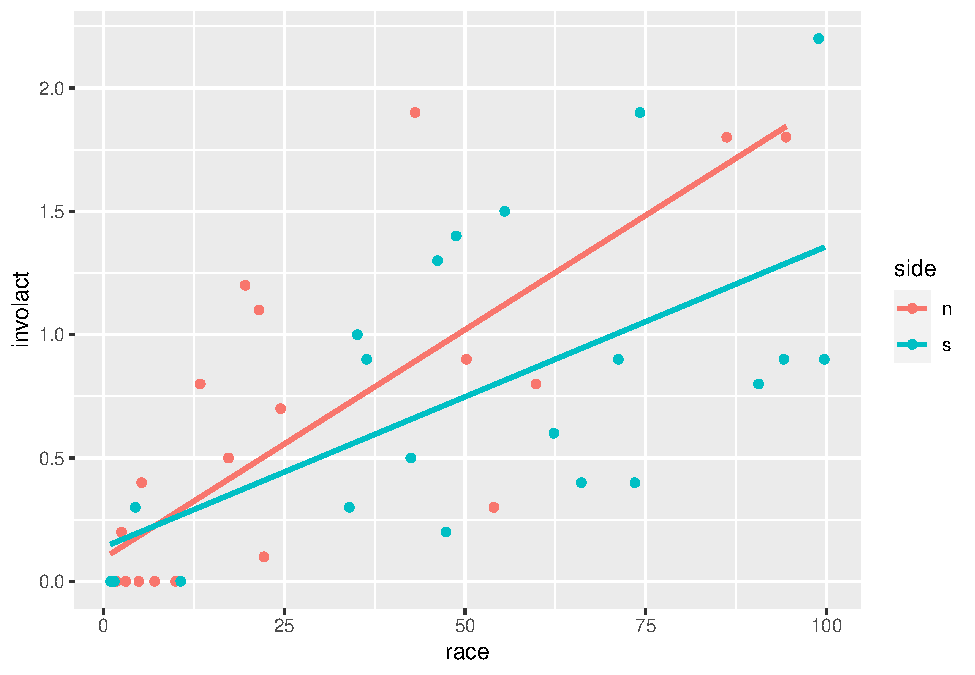
\includegraphics{intro_stats_files/figure-latex/unnamed-chunk-197-1.pdf}

\hypertarget{exercise-15-1}{%
\paragraph*{Exercise 15}\label{exercise-15-1}}
\addcontentsline{toc}{paragraph}{Exercise 15}

Although the slopes appear to be different, this is quite misleading. Focus on just the red dots. Which regression condition appears to be violated if we only consider the north side regression? How does that violation appear to affect the slope of the regression line?

Please write up your answer here.

\hypertarget{regression-your-turn}{%
\section{Your turn}\label{regression-your-turn}}

Let's revisit the \texttt{penguins} data. Imagine that it was much easier to measure body mass than it was to measure flipper length. (I'm not a penguin expert, so I don't know if that's true, but it seems plausible. Weighing a penguin can be done without human contact, for example.) Can we accurately predict flipper length from body mass? (This means that \texttt{flipper\_length\_mm} should be the response variable on the y-axis and \texttt{body\_mass\_g} should be the predictor variable on the x-axis.)

\hypertarget{exercise-16a}{%
\paragraph*{Exercise 16(a)}\label{exercise-16a}}
\addcontentsline{toc}{paragraph}{Exercise 16(a)}

Create a scatterplot of the data. Do \emph{not} include a regression line yet. (In other words, there should be no \texttt{geom\_smooth} in this plot.)

\begin{Shaded}
\begin{Highlighting}[]
\CommentTok{\# Add code here to create a scatterplot of the data}
\end{Highlighting}
\end{Shaded}

\hypertarget{exercise-16b}{%
\paragraph*{Exercise 16(b)}\label{exercise-16b}}
\addcontentsline{toc}{paragraph}{Exercise 16(b)}

Use the scatterplot above to check the first three conditions of regression.

\begin{enumerate}
\def\labelenumi{\arabic{enumi}.}
\tightlist
\item
\item
\item
\end{enumerate}

\hypertarget{exercise-16c}{%
\paragraph*{Exercise 16(c)}\label{exercise-16c}}
\addcontentsline{toc}{paragraph}{Exercise 16(c)}

As we're reasonably satisfied that the first three conditions are met and regression is worth pursuing, run the \texttt{lm} command to perform the regression analysis. Assign the output to the name \texttt{fl\_bm\_lm}. Be sure to type the variable name \texttt{fl\_bm\_lm} on its own line so that the output is printed in this file.

Then use \texttt{tidy}, \texttt{augment}, and \texttt{glance} respectively on the output. Assign the output to the names \texttt{fl\_bm\_tidy}, \texttt{fl\_bm\_aug}, and \texttt{fl\_bm\_glance}. Again, in each code chunk, type the output variable name on its own line to ensure that it prints in this file.

\begin{Shaded}
\begin{Highlighting}[]
\CommentTok{\# Add code here to generate and print regression output with lm}
\end{Highlighting}
\end{Shaded}

\begin{Shaded}
\begin{Highlighting}[]
\CommentTok{\# Add code here to "tidy" and print the output from lm}
\end{Highlighting}
\end{Shaded}

\begin{Shaded}
\begin{Highlighting}[]
\CommentTok{\# Add code here to "augment" and print the output from lm}
\end{Highlighting}
\end{Shaded}

\begin{Shaded}
\begin{Highlighting}[]
\CommentTok{\# Add code here to "glance" at and print the output from lm}
\end{Highlighting}
\end{Shaded}

\hypertarget{exercise-16d}{%
\paragraph*{Exercise 16(d)}\label{exercise-16d}}
\addcontentsline{toc}{paragraph}{Exercise 16(d)}

Use the \texttt{glance} output from above to create a residual plot with a blue horizontal reference line.

\begin{Shaded}
\begin{Highlighting}[]
\CommentTok{\# Add code here to create a residual plot}
\end{Highlighting}
\end{Shaded}

\hypertarget{exercise-16e}{%
\paragraph*{Exercise 16(e)}\label{exercise-16e}}
\addcontentsline{toc}{paragraph}{Exercise 16(e)}

Use the residual plot to check the fourth regression condition.

Please write up your answer here.

\hypertarget{exercise-16f}{%
\paragraph*{Exercise 16(f)}\label{exercise-16f}}
\addcontentsline{toc}{paragraph}{Exercise 16(f)}

With all the conditions met, plot the regression line on top of the scatterplot of the data. (Use \texttt{geom\_smooth} with \texttt{method\ =\ lm} and \texttt{se\ =\ FALSE} as in the examples earlier.)

\begin{Shaded}
\begin{Highlighting}[]
\CommentTok{\# Add code here to plot the regression line on the scatterplot}
\end{Highlighting}
\end{Shaded}

\hypertarget{exercise-16g}{%
\paragraph*{Exercise 16(g)}\label{exercise-16g}}
\addcontentsline{toc}{paragraph}{Exercise 16(g)}

Using the values of the intercept and slope from the \texttt{tidy} output, write the regression equation mathematically (enclosing your answer in double dollar signs as above), using contextually meaningful variable names.

\[
write-math-here
\]

\hypertarget{exercise-16h}{%
\paragraph*{Exercise 16(h)}\label{exercise-16h}}
\addcontentsline{toc}{paragraph}{Exercise 16(h)}

Interpret the slope in a full, contextually meaningful sentence.

Please write up your answer here.

\hypertarget{exercise-16i}{%
\paragraph*{Exercise 16(i)}\label{exercise-16i}}
\addcontentsline{toc}{paragraph}{Exercise 16(i)}

Give a literal interpretation of the intercept. Then comment on the appropriateness of that interpretation. (In other words, does the intercept make sense, or is it a case of extrapolation?)

Please write up your answer here.

\hypertarget{exercise-16j}{%
\paragraph*{Exercise 16(j)}\label{exercise-16j}}
\addcontentsline{toc}{paragraph}{Exercise 16(j)}

Use the equation of the regression line to predict the FAIR policy rate per 100 housing units for a ZIP code with 80\% racial minorities. Show your work. Then put that prediction into a full, contextually meaningful sentence.

Please write up your answer here.

\hypertarget{exercise-16k}{%
\paragraph*{Exercise 16(k)}\label{exercise-16k}}
\addcontentsline{toc}{paragraph}{Exercise 16(k)}

Using the value of \(R^2\) from the \texttt{glance} output, write a full, contextually meaningful sentence interpreting that value.

Please write up your answer here.

\hypertarget{exercise-16l}{%
\paragraph*{Exercise 16(l)}\label{exercise-16l}}
\addcontentsline{toc}{paragraph}{Exercise 16(l)}

Add \texttt{color\ =\ species} to the \texttt{aes} portion of the \texttt{ggplot} command to look at the regression lines for the three different species separately. Comment on the slopes of those three regression lines.

\begin{Shaded}
\begin{Highlighting}[]
\CommentTok{\# Add code here to plot regressions by species}
\end{Highlighting}
\end{Shaded}

Please write up your answer here.

\hypertarget{regression-conclusion}{%
\section{Conclusion}\label{regression-conclusion}}

Going beyond mere correlation, a regression analysis allows us to specify a linear model in the form of an equation. Assuming the conditions are met, this allows us to say more about the association. For example, the slope predicts how the response changes when comparing two values of the predictor. In fact, we can use the regression line to make a prediction for any reasonable value of the predictor (being careful not to extrapolate). Because regression is only a model, these predictions will not be exactly correct. Real data comes with residuals, meaning deviations from the idealized predictions of the model. But if those residuals are relatively small then the \(R^2\) value will be large and the model does a good job making reasonably accurate predictions.

\hypertarget{regression-prep}{%
\subsection{Preparing and submitting your assignment}\label{regression-prep}}

\begin{enumerate}
\def\labelenumi{\arabic{enumi}.}
\tightlist
\item
  From the ``Run'' menu, select ``Restart R and Run All Chunks''.
\item
  Deal with any code errors that crop up. Repeat steps 1---2 until there are no more code errors.
\item
  Spell check your document by clicking the icon with ``ABC'' and a check mark.
\item
  Hit the ``Preview'' button one last time to generate the final draft of the \texttt{.nb.html} file.
\item
  Proofread the HTML file carefully. If there are errors, go back and fix them, then repeat steps 1--5 again.
\end{enumerate}

If you have completed this chapter as part of a statistics course, follow the directions you receive from your professor to submit your assignment.

\hypertarget{randomization1}{%
\chapter{Introduction to randomization, Part 1}\label{randomization1}}

2.0

\hypertarget{functions-introduced-in-this-chapter-7}{%
\subsection*{Functions introduced in this chapter}\label{functions-introduced-in-this-chapter-7}}
\addcontentsline{toc}{subsection}{Functions introduced in this chapter}

\texttt{set.seed}, \texttt{rflip}, \texttt{do}

\hypertarget{randomization1-intro}{%
\section{Introduction}\label{randomization1-intro}}

In this module, we'll learn about randomization and simulation. When we want to understand how sampling works, it's helpful to simulate the process of drawing samples repeatedly from a population. In the days before computing, this was very difficult to do. Now, a few simple lines of computer code can generate thousands (even millions) of random samples, often in a matter of seconds or less.

\hypertarget{randomization1-install}{%
\subsection{Install new packages}\label{randomization1-install}}

If you are using RStudio Workbench, you do not need to install any packages. (Any packages you need should already be installed by the server administrators.)

If you are using R and RStudio on your own machine instead of accessing RStudio Workbench through a browser, you'll need to type the following command at the Console:

\begin{verbatim}
install.packages("mosaic")
\end{verbatim}

\hypertarget{randomization1-download}{%
\subsection{Download the R notebook file}\label{randomization1-download}}

Check the upper-right corner in RStudio to make sure you're in your \texttt{intro\_stats} project. Then click on the following link to download this chapter as an R notebook file (\texttt{.Rmd}).

https://vectorposse.github.io/intro\_stats/chapter\_downloads/08-intro\_to\_randomization\_1.Rmd

Once the file is downloaded, move it to your project folder in RStudio and open it there.

\hypertarget{randomization1-restart}{%
\subsection{Restart R and run all chunks}\label{randomization1-restart}}

In RStudio, select ``Restart R and Run All Chunks'' from the ``Run'' menu.

\hypertarget{randomization1-load}{%
\subsection{Load packages}\label{randomization1-load}}

We load the \texttt{tidyverse} package. The \texttt{mosaic} package contains some tools for making it easier to learn about randomization and simulation.

\begin{Shaded}
\begin{Highlighting}[]
\FunctionTok{library}\NormalTok{(tidyverse)}
\FunctionTok{library}\NormalTok{(mosaic)}
\end{Highlighting}
\end{Shaded}

\begin{verbatim}
## Registered S3 method overwritten by 'mosaic':
##   method                           from   
##   fortify.SpatialPolygonsDataFrame ggplot2
\end{verbatim}

\begin{verbatim}
## 
## The 'mosaic' package masks several functions from core packages in order to add 
## additional features.  The original behavior of these functions should not be affected by this.
\end{verbatim}

\begin{verbatim}
## 
## Attaching package: 'mosaic'
\end{verbatim}

\begin{verbatim}
## The following object is masked from 'package:Matrix':
## 
##     mean
\end{verbatim}

\begin{verbatim}
## The following objects are masked from 'package:faraway':
## 
##     ilogit, logit
\end{verbatim}

\begin{verbatim}
## The following objects are masked from 'package:dplyr':
## 
##     count, do, tally
\end{verbatim}

\begin{verbatim}
## The following object is masked from 'package:purrr':
## 
##     cross
\end{verbatim}

\begin{verbatim}
## The following object is masked from 'package:ggplot2':
## 
##     stat
\end{verbatim}

\begin{verbatim}
## The following objects are masked from 'package:stats':
## 
##     binom.test, cor, cor.test, cov, fivenum, IQR, median, prop.test,
##     quantile, sd, t.test, var
\end{verbatim}

\begin{verbatim}
## The following objects are masked from 'package:base':
## 
##     max, mean, min, prod, range, sample, sum
\end{verbatim}

\hypertarget{randomization1-sample-pop}{%
\section{Sample and population}\label{randomization1-sample-pop}}

The goal of the next few chapters is to help you think about the process of sampling from a population. What do these terms mean?

A \emph{population} is a group of objects we would like to study. If that sounds vague, that's because it is. A population can be a group of any size and of any type of thing in which we're interested. Often, populations refer to groups of people. For example, in an election, the population of interest is all voters. But if you're a biologist, you might study populations of other kinds of organisms. If you're an engineer, you might study populations of bolts on bridges. If you're in finance, you might study populations of loans.

Populations are usually inaccessible in their entirety. It is impossible to survey every voter in any reasonably sized election, for example. Therefore, to study them, we have to collect a \emph{sample}. A sample is a subset of the population. We might conduct a poll of 2000 voters to try to learn about voting intentions for the entire population. Of course, for that to work, the sample has to be \emph{representative} of its population. We'll have more to say about that in the future.

\hypertarget{randomization1-coin}{%
\section{Flipping a coin}\label{randomization1-coin}}

Before we talk about how samples are obtained from populations in the real world, we're going to perform some simulations.

One of the simplest acts to simulate is flipping a coin. We could get an actual coin and physically flip it over and over again, but that is time-consuming and annoying. It is much easier to flip a ``virtual'' coin inside the computer. One way to accomplish this in R is to use the \texttt{rflip} command from the \texttt{mosaic} package.

One more bit of technical detail. Since there will be some randomness involved here, we will need to include an R command to ensure that we all get the same results every time this code runs. This is called ``setting the seed''. Don't worry too much about what this is doing under the hood. The basic idea is that two people who start with the same seed will generate the same sequence of ``random'' numbers.

The seed \texttt{1234} in the chunk below is totally arbitrary. It could have been any number at all. (And, in fact, we'll use different numbers just for fun.) If you change the seed, you will get different output, so we all need to use the same seed. But the actual common value we all use for the seed is irrelevant.

Here is one coin flip:

\begin{Shaded}
\begin{Highlighting}[]
\FunctionTok{set.seed}\NormalTok{(}\DecValTok{1234}\NormalTok{)}
\FunctionTok{rflip}\NormalTok{(}\DecValTok{1}\NormalTok{)}
\end{Highlighting}
\end{Shaded}

\begin{verbatim}
## 
## Flipping 1 coin [ Prob(Heads) = 0.5 ] ...
## 
## T
## 
## Number of Heads: 0 [Proportion Heads: 0]
\end{verbatim}

Here are ten coin flips:

\begin{Shaded}
\begin{Highlighting}[]
\FunctionTok{set.seed}\NormalTok{(}\DecValTok{1234}\NormalTok{)}
\FunctionTok{rflip}\NormalTok{(}\DecValTok{10}\NormalTok{)}
\end{Highlighting}
\end{Shaded}

\begin{verbatim}
## 
## Flipping 10 coins [ Prob(Heads) = 0.5 ] ...
## 
## T H H H H H T T H H
## 
## Number of Heads: 7 [Proportion Heads: 0.7]
\end{verbatim}

Just to confirm that this is a random process, let's flip ten coins again (but without setting the seed again):

\begin{Shaded}
\begin{Highlighting}[]
\FunctionTok{rflip}\NormalTok{(}\DecValTok{10}\NormalTok{)}
\end{Highlighting}
\end{Shaded}

\begin{verbatim}
## 
## Flipping 10 coins [ Prob(Heads) = 0.5 ] ...
## 
## H H T H T H T T T T
## 
## Number of Heads: 4 [Proportion Heads: 0.4]
\end{verbatim}

If we return to the previous seed of 1234, we should obtain the same ten coin flips we did at first:

\begin{Shaded}
\begin{Highlighting}[]
\FunctionTok{set.seed}\NormalTok{(}\DecValTok{1234}\NormalTok{)}
\FunctionTok{rflip}\NormalTok{(}\DecValTok{10}\NormalTok{)}
\end{Highlighting}
\end{Shaded}

\begin{verbatim}
## 
## Flipping 10 coins [ Prob(Heads) = 0.5 ] ...
## 
## T H H H H H T T H H
## 
## Number of Heads: 7 [Proportion Heads: 0.7]
\end{verbatim}

And just to see the effect of setting a different seed:

\begin{Shaded}
\begin{Highlighting}[]
\FunctionTok{set.seed}\NormalTok{(}\DecValTok{9999}\NormalTok{)}
\FunctionTok{rflip}\NormalTok{(}\DecValTok{10}\NormalTok{)}
\end{Highlighting}
\end{Shaded}

\begin{verbatim}
## 
## Flipping 10 coins [ Prob(Heads) = 0.5 ] ...
## 
## H H H T H H T H H H
## 
## Number of Heads: 8 [Proportion Heads: 0.8]
\end{verbatim}

\hypertarget{exercise-1-5}{%
\paragraph*{Exercise 1}\label{exercise-1-5}}
\addcontentsline{toc}{paragraph}{Exercise 1}

In ten coin flips, how many would you generally expect to come up heads? Is that the actual number of heads you saw in the simulations above? Why aren't the simulations coming up with the expected number of heads each time?

Please write up your answer here.

\hypertarget{randomization1-multiple}{%
\section{Multiple simulations}\label{randomization1-multiple}}

Suppose now that you are not the only person flipping coins. Suppose a bunch of people in a room are all flipping coins. We'll start with ten coin flips per person, a task that could be reasonably done even without a computer.

You might observe three heads in ten flips. Fine, but what about everyone else in the room? What numbers of heads will they see?

The \texttt{do} command from \texttt{mosaic} is a way of doing something multiple times. Imagine there are twenty people in the room, each flipping a coin ten times. Observe:

\begin{Shaded}
\begin{Highlighting}[]
\FunctionTok{set.seed}\NormalTok{(}\DecValTok{12345}\NormalTok{)}
\FunctionTok{do}\NormalTok{(}\DecValTok{20}\NormalTok{) }\SpecialCharTok{*} \FunctionTok{rflip}\NormalTok{(}\DecValTok{10}\NormalTok{)}
\end{Highlighting}
\end{Shaded}

\begin{verbatim}
##     n heads tails prop
## 1  10     2     8  0.2
## 2  10     5     5  0.5
## 3  10     5     5  0.5
## 4  10     4     6  0.4
## 5  10     4     6  0.4
## 6  10     7     3  0.7
## 7  10     6     4  0.6
## 8  10     5     5  0.5
## 9  10     7     3  0.7
## 10 10     7     3  0.7
## 11 10     6     4  0.6
## 12 10     7     3  0.7
## 13 10     7     3  0.7
## 14 10     6     4  0.6
## 15 10     7     3  0.7
## 16 10     6     4  0.6
## 17 10     7     3  0.7
## 18 10     3     7  0.3
## 19 10     4     6  0.4
## 20 10     7     3  0.7
\end{verbatim}

The syntax could not be any simpler: \texttt{do(20)\ *} means, literally, ``do twenty times.'' In other words, this command is telling R to repeat an action twenty times, where the action is flipping a single coin ten times.

You'll notice that in place of a list of outcomes (H or T) of all the individual flips, we have instead a summary of the number of heads and tails each person sees. Each row represents a person, and the columns give information about each person's flips. (There are \texttt{n\ =\ 10} flips for each person, but then the number of heads/tails---and the corresponding ``proportion'' of heads---changes from person to person.)

Looking at the above rows and columns, we see that the output of our little coin-flipping experiment is actually stored in a data frame! Let's give it a name and work with it.

\begin{Shaded}
\begin{Highlighting}[]
\FunctionTok{set.seed}\NormalTok{(}\DecValTok{12345}\NormalTok{)}
\NormalTok{coin\_flips\_20\_10 }\OtherTok{\textless{}{-}} \FunctionTok{do}\NormalTok{(}\DecValTok{20}\NormalTok{) }\SpecialCharTok{*} \FunctionTok{rflip}\NormalTok{(}\DecValTok{10}\NormalTok{)}
\NormalTok{coin\_flips\_20\_10}
\end{Highlighting}
\end{Shaded}

\begin{verbatim}
##     n heads tails prop
## 1  10     2     8  0.2
## 2  10     5     5  0.5
## 3  10     5     5  0.5
## 4  10     4     6  0.4
## 5  10     4     6  0.4
## 6  10     7     3  0.7
## 7  10     6     4  0.6
## 8  10     5     5  0.5
## 9  10     7     3  0.7
## 10 10     7     3  0.7
## 11 10     6     4  0.6
## 12 10     7     3  0.7
## 13 10     7     3  0.7
## 14 10     6     4  0.6
## 15 10     7     3  0.7
## 16 10     6     4  0.6
## 17 10     7     3  0.7
## 18 10     3     7  0.3
## 19 10     4     6  0.4
## 20 10     7     3  0.7
\end{verbatim}

It is significant that we can store our outcomes this way. Because we have a data frame, we can apply all our data analysis tools (graphs, charts, tables, summary statistics, etc.) to the ``data'' generated from our set of simulations.

For example, what is the mean number of heads these twenty people observed?

\begin{Shaded}
\begin{Highlighting}[]
\FunctionTok{mean}\NormalTok{(coin\_flips\_20\_10}\SpecialCharTok{$}\NormalTok{heads)}
\end{Highlighting}
\end{Shaded}

\begin{verbatim}
## [1] 5.6
\end{verbatim}

\hypertarget{exercise-2-4}{%
\paragraph*{Exercise 2}\label{exercise-2-4}}
\addcontentsline{toc}{paragraph}{Exercise 2}

The data frame \texttt{coin\_flips\_20\_10} contains four variables: \texttt{n}, \texttt{heads}, \texttt{tails}, and \texttt{prop}. In the code chunk above, we calculated \texttt{mean(coin\_flips\_20\_10\$heads)} which gave us the mean count of heads for all people flipping coins. Instead of calculating the mean count of heads, change the variable from \texttt{heads} to \texttt{prop} to calculate the mean \emph{proportion} of heads. Then explain why your answer makes sense in light of the mean count of heads calculated above.

\begin{Shaded}
\begin{Highlighting}[]
\CommentTok{\# Add code here to calculate the mean proportion of heads.}
\end{Highlighting}
\end{Shaded}

Please write up your answer here.

\begin{center}\rule{0.5\linewidth}{0.5pt}\end{center}

Let's look at a histogram of the number of heads we see in the simulated flips. (The fancy stuff in \texttt{scale\_x\_continuous} is just making sure that the x-axis goes from 0 to 10 and that the tick marks appear on each whole number.)

\begin{Shaded}
\begin{Highlighting}[]
\FunctionTok{ggplot}\NormalTok{(coin\_flips\_20\_10, }\FunctionTok{aes}\NormalTok{(}\AttributeTok{x =}\NormalTok{ heads)) }\SpecialCharTok{+}
    \FunctionTok{geom\_histogram}\NormalTok{(}\AttributeTok{binwidth =} \FloatTok{0.5}\NormalTok{) }\SpecialCharTok{+}
    \FunctionTok{scale\_x\_continuous}\NormalTok{(}\AttributeTok{limits =} \FunctionTok{c}\NormalTok{(}\SpecialCharTok{{-}}\DecValTok{1}\NormalTok{, }\DecValTok{11}\NormalTok{), }\AttributeTok{breaks =} \FunctionTok{seq}\NormalTok{(}\DecValTok{0}\NormalTok{, }\DecValTok{10}\NormalTok{, }\DecValTok{1}\NormalTok{))}
\end{Highlighting}
\end{Shaded}

\begin{verbatim}
## Warning: Removed 2 rows containing missing values (geom_bar).
\end{verbatim}

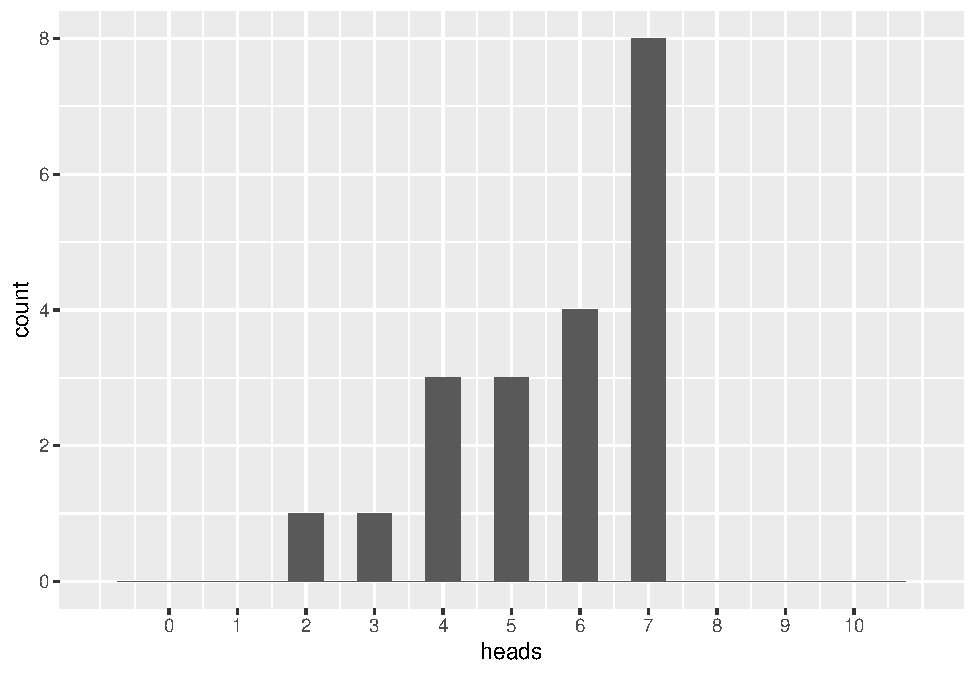
\includegraphics{intro_stats_files/figure-latex/unnamed-chunk-216-1.pdf}

Let's do the same thing, but now let's consider the \emph{proportion} of heads.

\begin{Shaded}
\begin{Highlighting}[]
\FunctionTok{ggplot}\NormalTok{(coin\_flips\_20\_10, }\FunctionTok{aes}\NormalTok{(}\AttributeTok{x =}\NormalTok{ prop)) }\SpecialCharTok{+}
    \FunctionTok{geom\_histogram}\NormalTok{(}\AttributeTok{binwidth =} \FloatTok{0.05}\NormalTok{) }\SpecialCharTok{+}
    \FunctionTok{scale\_x\_continuous}\NormalTok{(}\AttributeTok{limits =} \FunctionTok{c}\NormalTok{(}\SpecialCharTok{{-}}\FloatTok{0.1}\NormalTok{, }\FloatTok{1.1}\NormalTok{), }\AttributeTok{breaks =} \FunctionTok{seq}\NormalTok{(}\DecValTok{0}\NormalTok{, }\DecValTok{1}\NormalTok{, }\FloatTok{0.1}\NormalTok{))}
\end{Highlighting}
\end{Shaded}

\begin{verbatim}
## Warning: Removed 2 rows containing missing values (geom_bar).
\end{verbatim}

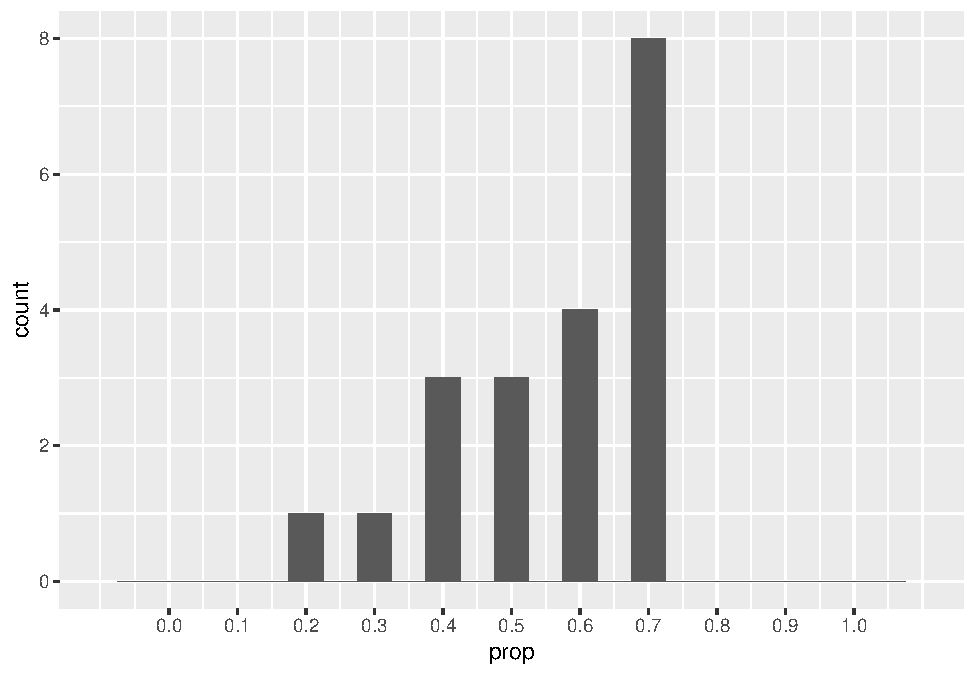
\includegraphics{intro_stats_files/figure-latex/unnamed-chunk-217-1.pdf}

\hypertarget{randomization1-bigger}{%
\section{Bigger and better!}\label{randomization1-bigger}}

With only twenty people, it was possible that, for example, nobody would get all heads or all tails. Indeed, in \texttt{coin\_flips\_20\_10} there were no people who got all heads or all tails. Also, there were more people with six and seven heads than with five heads, even though we ``expected'' the average to be five heads. There is nothing particularly significant about that; it happened by pure chance alone. Another run through the above commands would generate a somewhat different outcome. That's what happens when things are random.

Instead, let's imagine that we recruited way more people to flip coins with us. Let's try it again with 2000 people:

\begin{Shaded}
\begin{Highlighting}[]
\FunctionTok{set.seed}\NormalTok{(}\DecValTok{1234}\NormalTok{)}
\NormalTok{coin\_flips\_2000\_10 }\OtherTok{\textless{}{-}} \FunctionTok{do}\NormalTok{(}\DecValTok{2000}\NormalTok{) }\SpecialCharTok{*} \FunctionTok{rflip}\NormalTok{(}\DecValTok{10}\NormalTok{)}
\NormalTok{coin\_flips\_2000\_10}
\end{Highlighting}
\end{Shaded}

\begin{verbatim}
##       n heads tails prop
## 1    10     4     6  0.4
## 2    10     4     6  0.4
## 3    10     4     6  0.4
## 4    10     6     4  0.6
## 5    10     5     5  0.5
## 6    10     4     6  0.4
## 7    10     4     6  0.4
## 8    10     4     6  0.4
## 9    10     3     7  0.3
## 10   10     1     9  0.1
## 11   10     5     5  0.5
## 12   10     5     5  0.5
## 13   10     7     3  0.7
## 14   10     7     3  0.7
## 15   10     5     5  0.5
## 16   10     3     7  0.3
## 17   10     5     5  0.5
## 18   10     5     5  0.5
## 19   10     9     1  0.9
## 20   10     6     4  0.6
## 21   10     7     3  0.7
## 22   10     2     8  0.2
## 23   10     6     4  0.6
## 24   10     6     4  0.6
## 25   10     5     5  0.5
## 26   10     4     6  0.4
## 27   10     5     5  0.5
## 28   10     5     5  0.5
## 29   10     6     4  0.6
## 30   10     6     4  0.6
## 31   10     3     7  0.3
## 32   10     3     7  0.3
## 33   10     4     6  0.4
## 34   10     5     5  0.5
## 35   10     7     3  0.7
## 36   10     6     4  0.6
## 37   10     4     6  0.4
## 38   10     3     7  0.3
## 39   10     7     3  0.7
## 40   10     6     4  0.6
## 41   10     6     4  0.6
## 42   10     3     7  0.3
## 43   10     7     3  0.7
## 44   10     9     1  0.9
## 45   10     7     3  0.7
## 46   10     5     5  0.5
## 47   10     4     6  0.4
## 48   10     6     4  0.6
## 49   10     7     3  0.7
## 50   10     8     2  0.8
## 51   10     6     4  0.6
## 52   10     5     5  0.5
## 53   10     7     3  0.7
## 54   10     7     3  0.7
## 55   10     5     5  0.5
## 56   10     6     4  0.6
## 57   10     5     5  0.5
## 58   10     5     5  0.5
## 59   10     7     3  0.7
## 60   10     3     7  0.3
## 61   10     4     6  0.4
## 62   10     6     4  0.6
## 63   10     6     4  0.6
## 64   10     6     4  0.6
## 65   10     5     5  0.5
## 66   10     6     4  0.6
## 67   10     5     5  0.5
## 68   10     4     6  0.4
## 69   10     4     6  0.4
## 70   10     4     6  0.4
## 71   10     4     6  0.4
## 72   10     4     6  0.4
## 73   10     7     3  0.7
## 74   10     3     7  0.3
## 75   10     7     3  0.7
## 76   10     6     4  0.6
## 77   10     6     4  0.6
## 78   10     4     6  0.4
## 79   10     7     3  0.7
## 80   10     4     6  0.4
## 81   10     4     6  0.4
## 82   10     1     9  0.1
## 83   10     7     3  0.7
## 84   10     7     3  0.7
## 85   10     7     3  0.7
## 86   10     3     7  0.3
## 87   10     6     4  0.6
## 88   10     4     6  0.4
## 89   10     7     3  0.7
## 90   10     4     6  0.4
## 91   10     3     7  0.3
## 92   10     4     6  0.4
## 93   10     5     5  0.5
## 94   10     6     4  0.6
## 95   10     6     4  0.6
## 96   10     4     6  0.4
## 97   10     7     3  0.7
## 98   10     5     5  0.5
## 99   10     5     5  0.5
## 100  10     4     6  0.4
## 101  10     6     4  0.6
## 102  10     3     7  0.3
## 103  10     5     5  0.5
## 104  10     6     4  0.6
## 105  10     5     5  0.5
## 106  10     6     4  0.6
## 107  10     2     8  0.2
## 108  10     4     6  0.4
## 109  10     4     6  0.4
## 110  10     2     8  0.2
## 111  10     5     5  0.5
## 112  10     4     6  0.4
## 113  10     5     5  0.5
## 114  10     4     6  0.4
## 115  10     1     9  0.1
## 116  10     5     5  0.5
## 117  10     2     8  0.2
## 118  10     8     2  0.8
## 119  10     4     6  0.4
## 120  10     7     3  0.7
## 121  10     5     5  0.5
## 122  10     7     3  0.7
## 123  10     5     5  0.5
## 124  10     6     4  0.6
## 125  10     4     6  0.4
## 126  10     6     4  0.6
## 127  10     8     2  0.8
## 128  10     2     8  0.2
## 129  10     6     4  0.6
## 130  10     4     6  0.4
## 131  10     6     4  0.6
## 132  10     3     7  0.3
## 133  10     3     7  0.3
## 134  10     5     5  0.5
## 135  10     6     4  0.6
## 136  10     3     7  0.3
## 137  10     7     3  0.7
## 138  10     6     4  0.6
## 139  10     5     5  0.5
## 140  10     5     5  0.5
## 141  10     4     6  0.4
## 142  10     7     3  0.7
## 143  10     3     7  0.3
## 144  10     4     6  0.4
## 145  10     4     6  0.4
## 146  10     6     4  0.6
## 147  10     6     4  0.6
## 148  10     6     4  0.6
## 149  10     7     3  0.7
## 150  10     8     2  0.8
## 151  10     3     7  0.3
## 152  10     3     7  0.3
## 153  10     4     6  0.4
## 154  10     4     6  0.4
## 155  10     3     7  0.3
## 156  10     2     8  0.2
## 157  10     3     7  0.3
## 158  10     7     3  0.7
## 159  10     5     5  0.5
## 160  10     3     7  0.3
## 161  10     4     6  0.4
## 162  10     6     4  0.6
## 163  10     4     6  0.4
## 164  10     5     5  0.5
## 165  10     4     6  0.4
## 166  10     4     6  0.4
## 167  10     3     7  0.3
## 168  10     4     6  0.4
## 169  10     4     6  0.4
## 170  10     4     6  0.4
## 171  10     4     6  0.4
## 172  10     4     6  0.4
## 173  10     7     3  0.7
## 174  10     3     7  0.3
## 175  10     8     2  0.8
## 176  10     5     5  0.5
## 177  10     8     2  0.8
## 178  10     4     6  0.4
## 179  10     5     5  0.5
## 180  10     3     7  0.3
## 181  10     7     3  0.7
## 182  10     5     5  0.5
## 183  10     4     6  0.4
## 184  10     3     7  0.3
## 185  10     6     4  0.6
## 186  10     6     4  0.6
## 187  10     7     3  0.7
## 188  10     3     7  0.3
## 189  10     5     5  0.5
## 190  10     7     3  0.7
## 191  10     4     6  0.4
## 192  10     6     4  0.6
## 193  10     4     6  0.4
## 194  10     5     5  0.5
## 195  10     5     5  0.5
## 196  10     8     2  0.8
## 197  10     9     1  0.9
## 198  10     5     5  0.5
## 199  10     7     3  0.7
## 200  10     5     5  0.5
## 201  10     4     6  0.4
## 202  10     5     5  0.5
## 203  10     3     7  0.3
## 204  10     5     5  0.5
## 205  10     6     4  0.6
## 206  10     3     7  0.3
## 207  10     4     6  0.4
## 208  10     3     7  0.3
## 209  10     4     6  0.4
## 210  10     9     1  0.9
## 211  10     4     6  0.4
## 212  10     5     5  0.5
## 213  10     6     4  0.6
## 214  10     3     7  0.3
## 215  10     5     5  0.5
## 216  10     7     3  0.7
## 217  10     4     6  0.4
## 218  10     6     4  0.6
## 219  10     4     6  0.4
## 220  10     4     6  0.4
## 221  10     4     6  0.4
## 222  10     4     6  0.4
## 223  10    10     0  1.0
## 224  10     4     6  0.4
## 225  10     3     7  0.3
## 226  10     8     2  0.8
## 227  10     7     3  0.7
## 228  10     6     4  0.6
## 229  10     6     4  0.6
## 230  10     4     6  0.4
## 231  10     6     4  0.6
## 232  10     4     6  0.4
## 233  10     6     4  0.6
## 234  10     3     7  0.3
## 235  10     4     6  0.4
## 236  10     4     6  0.4
## 237  10     5     5  0.5
## 238  10     3     7  0.3
## 239  10     4     6  0.4
## 240  10     7     3  0.7
## 241  10     8     2  0.8
## 242  10     6     4  0.6
## 243  10     6     4  0.6
## 244  10     7     3  0.7
## 245  10     6     4  0.6
## 246  10     6     4  0.6
## 247  10     8     2  0.8
## 248  10     4     6  0.4
## 249  10     4     6  0.4
## 250  10     4     6  0.4
## 251  10     4     6  0.4
## 252  10     5     5  0.5
## 253  10     5     5  0.5
## 254  10     3     7  0.3
## 255  10     4     6  0.4
## 256  10     5     5  0.5
## 257  10     6     4  0.6
## 258  10     6     4  0.6
## 259  10     6     4  0.6
## 260  10     8     2  0.8
## 261  10     5     5  0.5
## 262  10     5     5  0.5
## 263  10     1     9  0.1
## 264  10     6     4  0.6
## 265  10     3     7  0.3
## 266  10     4     6  0.4
## 267  10     6     4  0.6
## 268  10     7     3  0.7
## 269  10     7     3  0.7
## 270  10     5     5  0.5
## 271  10     5     5  0.5
## 272  10     5     5  0.5
## 273  10     5     5  0.5
## 274  10     6     4  0.6
## 275  10     5     5  0.5
## 276  10     6     4  0.6
## 277  10     6     4  0.6
## 278  10     5     5  0.5
## 279  10     5     5  0.5
## 280  10     5     5  0.5
## 281  10    10     0  1.0
## 282  10     5     5  0.5
## 283  10     7     3  0.7
## 284  10     4     6  0.4
## 285  10     5     5  0.5
## 286  10     6     4  0.6
## 287  10     6     4  0.6
## 288  10     3     7  0.3
## 289  10     6     4  0.6
## 290  10     5     5  0.5
## 291  10     7     3  0.7
## 292  10     4     6  0.4
## 293  10     4     6  0.4
## 294  10     3     7  0.3
## 295  10     8     2  0.8
## 296  10     2     8  0.2
## 297  10     5     5  0.5
## 298  10     4     6  0.4
## 299  10     7     3  0.7
## 300  10     3     7  0.3
## 301  10     3     7  0.3
## 302  10     6     4  0.6
## 303  10     6     4  0.6
## 304  10     6     4  0.6
## 305  10     4     6  0.4
## 306  10     5     5  0.5
## 307  10     4     6  0.4
## 308  10     5     5  0.5
## 309  10     3     7  0.3
## 310  10     6     4  0.6
## 311  10     6     4  0.6
## 312  10     5     5  0.5
## 313  10     4     6  0.4
## 314  10     3     7  0.3
## 315  10     5     5  0.5
## 316  10     3     7  0.3
## 317  10     4     6  0.4
## 318  10     6     4  0.6
## 319  10     4     6  0.4
## 320  10     2     8  0.2
## 321  10     5     5  0.5
## 322  10     6     4  0.6
## 323  10     4     6  0.4
## 324  10     6     4  0.6
## 325  10     4     6  0.4
## 326  10     4     6  0.4
## 327  10     6     4  0.6
## 328  10     5     5  0.5
## 329  10     7     3  0.7
## 330  10     4     6  0.4
## 331  10     3     7  0.3
## 332  10     4     6  0.4
## 333  10     5     5  0.5
## 334  10     5     5  0.5
## 335  10     6     4  0.6
## 336  10     4     6  0.4
## 337  10     3     7  0.3
## 338  10     6     4  0.6
## 339  10     4     6  0.4
## 340  10     2     8  0.2
## 341  10     7     3  0.7
## 342  10     3     7  0.3
## 343  10     6     4  0.6
## 344  10     4     6  0.4
## 345  10     0    10  0.0
## 346  10     3     7  0.3
## 347  10     6     4  0.6
## 348  10     5     5  0.5
## 349  10     7     3  0.7
## 350  10     3     7  0.3
## 351  10     6     4  0.6
## 352  10     7     3  0.7
## 353  10     6     4  0.6
## 354  10     8     2  0.8
## 355  10     6     4  0.6
## 356  10     4     6  0.4
## 357  10     8     2  0.8
## 358  10     2     8  0.2
## 359  10     4     6  0.4
## 360  10     6     4  0.6
## 361  10     2     8  0.2
## 362  10     4     6  0.4
## 363  10     5     5  0.5
## 364  10     4     6  0.4
## 365  10     7     3  0.7
## 366  10     6     4  0.6
## 367  10     6     4  0.6
## 368  10     2     8  0.2
## 369  10     4     6  0.4
## 370  10     6     4  0.6
## 371  10     2     8  0.2
## 372  10     4     6  0.4
## 373  10     2     8  0.2
## 374  10     4     6  0.4
## 375  10     8     2  0.8
## 376  10     6     4  0.6
## 377  10     6     4  0.6
## 378  10     6     4  0.6
## 379  10     6     4  0.6
## 380  10     6     4  0.6
## 381  10     6     4  0.6
## 382  10     8     2  0.8
## 383  10     4     6  0.4
## 384  10     6     4  0.6
## 385  10     4     6  0.4
## 386  10     3     7  0.3
## 387  10     6     4  0.6
## 388  10     4     6  0.4
## 389  10     6     4  0.6
## 390  10     5     5  0.5
## 391  10     4     6  0.4
## 392  10     6     4  0.6
## 393  10     6     4  0.6
## 394  10     5     5  0.5
## 395  10     4     6  0.4
## 396  10     6     4  0.6
## 397  10     4     6  0.4
## 398  10     7     3  0.7
## 399  10     4     6  0.4
## 400  10     6     4  0.6
## 401  10     3     7  0.3
## 402  10     6     4  0.6
## 403  10     7     3  0.7
## 404  10     4     6  0.4
## 405  10     6     4  0.6
## 406  10     3     7  0.3
## 407  10     7     3  0.7
## 408  10     8     2  0.8
## 409  10     4     6  0.4
## 410  10     6     4  0.6
## 411  10     4     6  0.4
## 412  10     3     7  0.3
## 413  10     4     6  0.4
## 414  10     7     3  0.7
## 415  10     3     7  0.3
## 416  10     5     5  0.5
## 417  10     5     5  0.5
## 418  10     7     3  0.7
## 419  10     6     4  0.6
## 420  10     5     5  0.5
## 421  10     6     4  0.6
## 422  10     3     7  0.3
## 423  10     5     5  0.5
## 424  10     4     6  0.4
## 425  10     5     5  0.5
## 426  10     5     5  0.5
## 427  10     3     7  0.3
## 428  10     6     4  0.6
## 429  10     4     6  0.4
## 430  10     6     4  0.6
## 431  10     7     3  0.7
## 432  10     7     3  0.7
## 433  10     5     5  0.5
## 434  10     4     6  0.4
## 435  10     4     6  0.4
## 436  10     3     7  0.3
## 437  10     4     6  0.4
## 438  10     5     5  0.5
## 439  10     7     3  0.7
## 440  10     5     5  0.5
## 441  10     5     5  0.5
## 442  10     7     3  0.7
## 443  10     8     2  0.8
## 444  10     6     4  0.6
## 445  10     5     5  0.5
## 446  10     4     6  0.4
## 447  10     3     7  0.3
## 448  10     5     5  0.5
## 449  10     6     4  0.6
## 450  10     7     3  0.7
## 451  10     9     1  0.9
## 452  10     5     5  0.5
## 453  10     5     5  0.5
## 454  10     3     7  0.3
## 455  10     5     5  0.5
## 456  10     5     5  0.5
## 457  10     5     5  0.5
## 458  10     3     7  0.3
## 459  10     3     7  0.3
## 460  10     5     5  0.5
## 461  10     4     6  0.4
## 462  10     7     3  0.7
## 463  10     7     3  0.7
## 464  10     3     7  0.3
## 465  10     4     6  0.4
## 466  10     5     5  0.5
## 467  10     5     5  0.5
## 468  10     3     7  0.3
## 469  10     8     2  0.8
## 470  10     5     5  0.5
## 471  10     6     4  0.6
## 472  10     5     5  0.5
## 473  10     7     3  0.7
## 474  10     4     6  0.4
## 475  10     4     6  0.4
## 476  10     5     5  0.5
## 477  10     2     8  0.2
## 478  10     6     4  0.6
## 479  10     6     4  0.6
## 480  10     2     8  0.2
## 481  10     6     4  0.6
## 482  10     5     5  0.5
## 483  10     5     5  0.5
## 484  10     6     4  0.6
## 485  10     4     6  0.4
## 486  10     5     5  0.5
## 487  10     6     4  0.6
## 488  10     3     7  0.3
## 489  10     3     7  0.3
## 490  10     6     4  0.6
## 491  10     4     6  0.4
## 492  10     7     3  0.7
## 493  10     4     6  0.4
## 494  10     6     4  0.6
## 495  10     4     6  0.4
## 496  10     8     2  0.8
## 497  10     5     5  0.5
## 498  10     6     4  0.6
## 499  10     6     4  0.6
## 500  10     4     6  0.4
## 501  10     4     6  0.4
## 502  10     5     5  0.5
## 503  10     3     7  0.3
## 504  10     3     7  0.3
## 505  10     6     4  0.6
## 506  10     5     5  0.5
## 507  10     6     4  0.6
## 508  10     5     5  0.5
## 509  10     5     5  0.5
## 510  10     6     4  0.6
## 511  10     5     5  0.5
## 512  10     4     6  0.4
## 513  10     6     4  0.6
## 514  10     5     5  0.5
## 515  10     5     5  0.5
## 516  10     9     1  0.9
## 517  10     4     6  0.4
## 518  10     2     8  0.2
## 519  10     3     7  0.3
## 520  10     4     6  0.4
## 521  10     2     8  0.2
## 522  10     6     4  0.6
## 523  10     6     4  0.6
## 524  10     7     3  0.7
## 525  10     5     5  0.5
## 526  10     7     3  0.7
## 527  10     7     3  0.7
## 528  10     2     8  0.2
## 529  10     4     6  0.4
## 530  10     8     2  0.8
## 531  10     5     5  0.5
## 532  10     6     4  0.6
## 533  10     8     2  0.8
## 534  10     3     7  0.3
## 535  10     4     6  0.4
## 536  10     6     4  0.6
## 537  10     8     2  0.8
## 538  10     4     6  0.4
## 539  10     4     6  0.4
## 540  10     6     4  0.6
## 541  10     5     5  0.5
## 542  10     4     6  0.4
## 543  10     5     5  0.5
## 544  10     5     5  0.5
## 545  10     3     7  0.3
## 546  10     4     6  0.4
## 547  10     6     4  0.6
## 548  10     4     6  0.4
## 549  10     6     4  0.6
## 550  10     4     6  0.4
## 551  10     6     4  0.6
## 552  10     3     7  0.3
## 553  10     5     5  0.5
## 554  10     6     4  0.6
## 555  10     5     5  0.5
## 556  10     8     2  0.8
## 557  10     2     8  0.2
## 558  10     5     5  0.5
## 559  10     4     6  0.4
## 560  10     5     5  0.5
## 561  10     4     6  0.4
## 562  10     6     4  0.6
## 563  10     6     4  0.6
## 564  10     4     6  0.4
## 565  10     2     8  0.2
## 566  10     3     7  0.3
## 567  10     6     4  0.6
## 568  10     3     7  0.3
## 569  10     5     5  0.5
## 570  10     7     3  0.7
## 571  10     8     2  0.8
## 572  10     6     4  0.6
## 573  10     4     6  0.4
## 574  10     6     4  0.6
## 575  10     3     7  0.3
## 576  10     4     6  0.4
## 577  10     5     5  0.5
## 578  10     7     3  0.7
## 579  10     4     6  0.4
## 580  10     4     6  0.4
## 581  10     2     8  0.2
## 582  10     6     4  0.6
## 583  10     5     5  0.5
## 584  10     5     5  0.5
## 585  10     5     5  0.5
## 586  10     6     4  0.6
## 587  10     6     4  0.6
## 588  10     8     2  0.8
## 589  10     5     5  0.5
## 590  10     8     2  0.8
## 591  10     5     5  0.5
## 592  10     6     4  0.6
## 593  10     7     3  0.7
## 594  10     3     7  0.3
## 595  10     4     6  0.4
## 596  10     2     8  0.2
## 597  10     5     5  0.5
## 598  10     6     4  0.6
## 599  10     6     4  0.6
## 600  10     7     3  0.7
## 601  10     4     6  0.4
## 602  10     6     4  0.6
## 603  10     6     4  0.6
## 604  10     5     5  0.5
## 605  10     5     5  0.5
## 606  10     7     3  0.7
## 607  10     7     3  0.7
## 608  10     6     4  0.6
## 609  10     3     7  0.3
## 610  10     4     6  0.4
## 611  10     9     1  0.9
## 612  10     6     4  0.6
## 613  10     5     5  0.5
## 614  10     4     6  0.4
## 615  10     6     4  0.6
## 616  10     4     6  0.4
## 617  10     7     3  0.7
## 618  10     3     7  0.3
## 619  10     6     4  0.6
## 620  10     5     5  0.5
## 621  10     7     3  0.7
## 622  10     5     5  0.5
## 623  10     5     5  0.5
## 624  10     5     5  0.5
## 625  10     6     4  0.6
## 626  10     3     7  0.3
## 627  10     4     6  0.4
## 628  10     8     2  0.8
## 629  10     6     4  0.6
## 630  10     6     4  0.6
## 631  10     5     5  0.5
## 632  10     3     7  0.3
## 633  10     5     5  0.5
## 634  10     4     6  0.4
## 635  10     6     4  0.6
## 636  10     7     3  0.7
## 637  10     5     5  0.5
## 638  10     4     6  0.4
## 639  10     4     6  0.4
## 640  10     5     5  0.5
## 641  10     3     7  0.3
## 642  10     4     6  0.4
## 643  10     5     5  0.5
## 644  10     7     3  0.7
## 645  10     5     5  0.5
## 646  10     5     5  0.5
## 647  10     5     5  0.5
## 648  10     4     6  0.4
## 649  10     5     5  0.5
## 650  10     7     3  0.7
## 651  10     3     7  0.3
## 652  10     6     4  0.6
## 653  10     6     4  0.6
## 654  10     8     2  0.8
## 655  10     7     3  0.7
## 656  10     4     6  0.4
## 657  10     7     3  0.7
## 658  10     5     5  0.5
## 659  10     7     3  0.7
## 660  10     6     4  0.6
## 661  10     2     8  0.2
## 662  10     8     2  0.8
## 663  10     2     8  0.2
## 664  10     6     4  0.6
## 665  10     4     6  0.4
## 666  10     3     7  0.3
## 667  10     5     5  0.5
## 668  10     6     4  0.6
## 669  10     6     4  0.6
## 670  10     4     6  0.4
## 671  10     7     3  0.7
## 672  10     2     8  0.2
## 673  10     2     8  0.2
## 674  10     6     4  0.6
## 675  10     5     5  0.5
## 676  10     8     2  0.8
## 677  10     5     5  0.5
## 678  10     5     5  0.5
## 679  10     5     5  0.5
## 680  10     5     5  0.5
## 681  10     6     4  0.6
## 682  10     4     6  0.4
## 683  10     2     8  0.2
## 684  10     6     4  0.6
## 685  10     4     6  0.4
## 686  10     5     5  0.5
## 687  10     5     5  0.5
## 688  10     6     4  0.6
## 689  10     6     4  0.6
## 690  10     4     6  0.4
## 691  10     4     6  0.4
## 692  10     4     6  0.4
## 693  10     5     5  0.5
## 694  10     5     5  0.5
## 695  10     5     5  0.5
## 696  10     5     5  0.5
## 697  10     6     4  0.6
## 698  10     6     4  0.6
## 699  10     5     5  0.5
## 700  10     7     3  0.7
## 701  10     2     8  0.2
## 702  10     7     3  0.7
## 703  10     7     3  0.7
## 704  10     1     9  0.1
## 705  10     5     5  0.5
## 706  10     5     5  0.5
## 707  10     4     6  0.4
## 708  10     4     6  0.4
## 709  10     6     4  0.6
## 710  10     3     7  0.3
## 711  10     4     6  0.4
## 712  10     5     5  0.5
## 713  10     8     2  0.8
## 714  10     3     7  0.3
## 715  10     6     4  0.6
## 716  10     5     5  0.5
## 717  10     4     6  0.4
## 718  10     2     8  0.2
## 719  10     3     7  0.3
## 720  10     1     9  0.1
## 721  10     3     7  0.3
## 722  10     6     4  0.6
## 723  10     3     7  0.3
## 724  10     5     5  0.5
## 725  10     5     5  0.5
## 726  10     7     3  0.7
## 727  10     7     3  0.7
## 728  10     3     7  0.3
## 729  10     4     6  0.4
## 730  10     5     5  0.5
## 731  10     7     3  0.7
## 732  10     6     4  0.6
## 733  10     7     3  0.7
## 734  10     8     2  0.8
## 735  10     6     4  0.6
## 736  10     2     8  0.2
## 737  10     6     4  0.6
## 738  10     6     4  0.6
## 739  10     5     5  0.5
## 740  10     4     6  0.4
## 741  10     6     4  0.6
## 742  10     5     5  0.5
## 743  10     5     5  0.5
## 744  10     4     6  0.4
## 745  10     5     5  0.5
## 746  10     4     6  0.4
## 747  10     3     7  0.3
## 748  10     5     5  0.5
## 749  10     6     4  0.6
## 750  10     6     4  0.6
## 751  10     7     3  0.7
## 752  10     4     6  0.4
## 753  10     4     6  0.4
## 754  10     5     5  0.5
## 755  10     6     4  0.6
## 756  10     6     4  0.6
## 757  10     3     7  0.3
## 758  10     5     5  0.5
## 759  10     4     6  0.4
## 760  10     5     5  0.5
## 761  10     5     5  0.5
## 762  10     5     5  0.5
## 763  10     5     5  0.5
## 764  10     4     6  0.4
## 765  10     5     5  0.5
## 766  10     5     5  0.5
## 767  10     5     5  0.5
## 768  10     5     5  0.5
## 769  10     7     3  0.7
## 770  10     3     7  0.3
## 771  10     2     8  0.2
## 772  10     6     4  0.6
## 773  10     8     2  0.8
## 774  10     5     5  0.5
## 775  10     7     3  0.7
## 776  10     6     4  0.6
## 777  10     5     5  0.5
## 778  10     7     3  0.7
## 779  10     3     7  0.3
## 780  10     5     5  0.5
## 781  10     6     4  0.6
## 782  10     3     7  0.3
## 783  10     4     6  0.4
## 784  10     5     5  0.5
## 785  10     5     5  0.5
## 786  10     7     3  0.7
## 787  10     5     5  0.5
## 788  10     5     5  0.5
## 789  10     2     8  0.2
## 790  10     6     4  0.6
## 791  10     5     5  0.5
## 792  10     8     2  0.8
## 793  10     5     5  0.5
## 794  10     4     6  0.4
## 795  10     6     4  0.6
## 796  10     5     5  0.5
## 797  10     7     3  0.7
## 798  10     6     4  0.6
## 799  10     5     5  0.5
## 800  10     5     5  0.5
## 801  10     3     7  0.3
## 802  10     4     6  0.4
## 803  10     3     7  0.3
## 804  10     3     7  0.3
## 805  10     3     7  0.3
## 806  10     5     5  0.5
## 807  10     5     5  0.5
## 808  10     7     3  0.7
## 809  10     4     6  0.4
## 810  10     7     3  0.7
## 811  10     5     5  0.5
## 812  10     5     5  0.5
## 813  10     5     5  0.5
## 814  10     5     5  0.5
## 815  10     5     5  0.5
## 816  10     4     6  0.4
## 817  10     7     3  0.7
## 818  10     4     6  0.4
## 819  10     4     6  0.4
## 820  10     3     7  0.3
## 821  10     6     4  0.6
## 822  10     6     4  0.6
## 823  10     6     4  0.6
## 824  10     8     2  0.8
## 825  10     3     7  0.3
## 826  10     3     7  0.3
## 827  10     6     4  0.6
## 828  10     7     3  0.7
## 829  10     5     5  0.5
## 830  10     3     7  0.3
## 831  10     6     4  0.6
## 832  10     6     4  0.6
## 833  10     5     5  0.5
## 834  10     6     4  0.6
## 835  10     5     5  0.5
## 836  10     8     2  0.8
## 837  10     5     5  0.5
## 838  10     5     5  0.5
## 839  10     3     7  0.3
## 840  10     2     8  0.2
## 841  10     4     6  0.4
## 842  10     6     4  0.6
## 843  10     7     3  0.7
## 844  10     7     3  0.7
## 845  10     3     7  0.3
## 846  10     3     7  0.3
## 847  10     3     7  0.3
## 848  10     4     6  0.4
## 849  10     5     5  0.5
## 850  10     6     4  0.6
## 851  10     4     6  0.4
## 852  10     3     7  0.3
## 853  10     4     6  0.4
## 854  10     5     5  0.5
## 855  10     4     6  0.4
## 856  10     6     4  0.6
## 857  10     6     4  0.6
## 858  10     7     3  0.7
## 859  10     5     5  0.5
## 860  10     5     5  0.5
## 861  10     4     6  0.4
## 862  10     6     4  0.6
## 863  10     4     6  0.4
## 864  10     6     4  0.6
## 865  10     6     4  0.6
## 866  10     6     4  0.6
## 867  10     2     8  0.2
## 868  10     4     6  0.4
## 869  10     3     7  0.3
## 870  10     5     5  0.5
## 871  10     7     3  0.7
## 872  10     5     5  0.5
## 873  10     5     5  0.5
## 874  10     4     6  0.4
## 875  10     6     4  0.6
## 876  10     7     3  0.7
## 877  10     4     6  0.4
## 878  10     3     7  0.3
## 879  10     5     5  0.5
## 880  10     7     3  0.7
## 881  10     6     4  0.6
## 882  10     7     3  0.7
## 883  10     8     2  0.8
## 884  10     6     4  0.6
## 885  10     3     7  0.3
## 886  10     6     4  0.6
## 887  10     4     6  0.4
## 888  10     4     6  0.4
## 889  10     5     5  0.5
## 890  10     5     5  0.5
## 891  10     7     3  0.7
## 892  10     5     5  0.5
## 893  10     7     3  0.7
## 894  10     5     5  0.5
## 895  10     6     4  0.6
## 896  10     3     7  0.3
## 897  10     6     4  0.6
## 898  10     4     6  0.4
## 899  10     4     6  0.4
## 900  10     2     8  0.2
## 901  10     7     3  0.7
## 902  10     7     3  0.7
## 903  10     6     4  0.6
## 904  10     7     3  0.7
## 905  10     4     6  0.4
## 906  10     3     7  0.3
## 907  10     3     7  0.3
## 908  10     3     7  0.3
## 909  10     6     4  0.6
## 910  10     5     5  0.5
## 911  10     5     5  0.5
## 912  10     8     2  0.8
## 913  10     7     3  0.7
## 914  10     5     5  0.5
## 915  10     3     7  0.3
## 916  10     6     4  0.6
## 917  10     3     7  0.3
## 918  10     6     4  0.6
## 919  10     4     6  0.4
## 920  10     8     2  0.8
## 921  10     5     5  0.5
## 922  10     6     4  0.6
## 923  10     2     8  0.2
## 924  10     6     4  0.6
## 925  10     3     7  0.3
## 926  10     5     5  0.5
## 927  10     4     6  0.4
## 928  10     3     7  0.3
## 929  10     6     4  0.6
## 930  10     5     5  0.5
## 931  10     5     5  0.5
## 932  10     4     6  0.4
## 933  10     4     6  0.4
## 934  10     4     6  0.4
## 935  10     7     3  0.7
## 936  10     3     7  0.3
## 937  10     2     8  0.2
## 938  10     5     5  0.5
## 939  10     3     7  0.3
## 940  10     6     4  0.6
## 941  10     5     5  0.5
## 942  10     6     4  0.6
## 943  10     5     5  0.5
## 944  10     4     6  0.4
## 945  10     4     6  0.4
## 946  10     3     7  0.3
## 947  10     3     7  0.3
## 948  10     4     6  0.4
## 949  10     4     6  0.4
## 950  10     5     5  0.5
## 951  10     9     1  0.9
## 952  10     3     7  0.3
## 953  10     7     3  0.7
## 954  10     8     2  0.8
## 955  10     7     3  0.7
## 956  10     6     4  0.6
## 957  10     5     5  0.5
## 958  10     5     5  0.5
## 959  10     7     3  0.7
## 960  10     5     5  0.5
## 961  10     4     6  0.4
## 962  10     5     5  0.5
## 963  10     7     3  0.7
## 964  10     5     5  0.5
## 965  10     4     6  0.4
## 966  10     5     5  0.5
## 967  10     8     2  0.8
## 968  10     5     5  0.5
## 969  10     4     6  0.4
## 970  10     6     4  0.6
## 971  10     6     4  0.6
## 972  10     3     7  0.3
## 973  10     5     5  0.5
## 974  10     4     6  0.4
## 975  10     6     4  0.6
## 976  10     4     6  0.4
## 977  10     4     6  0.4
## 978  10     5     5  0.5
## 979  10     8     2  0.8
## 980  10     5     5  0.5
## 981  10     6     4  0.6
## 982  10     5     5  0.5
## 983  10     4     6  0.4
## 984  10     3     7  0.3
## 985  10     7     3  0.7
## 986  10     6     4  0.6
## 987  10     4     6  0.4
## 988  10     4     6  0.4
## 989  10     4     6  0.4
## 990  10     5     5  0.5
## 991  10     7     3  0.7
## 992  10     2     8  0.2
## 993  10     4     6  0.4
## 994  10     5     5  0.5
## 995  10     5     5  0.5
## 996  10     4     6  0.4
## 997  10     7     3  0.7
## 998  10     4     6  0.4
## 999  10     4     6  0.4
## 1000 10     2     8  0.2
## 1001 10     8     2  0.8
## 1002 10     5     5  0.5
## 1003 10     4     6  0.4
## 1004 10     6     4  0.6
## 1005 10     5     5  0.5
## 1006 10     3     7  0.3
## 1007 10     7     3  0.7
## 1008 10     5     5  0.5
## 1009 10     6     4  0.6
## 1010 10     5     5  0.5
## 1011 10     6     4  0.6
## 1012 10     7     3  0.7
## 1013 10     4     6  0.4
## 1014 10     3     7  0.3
## 1015 10     7     3  0.7
## 1016 10     5     5  0.5
## 1017 10     7     3  0.7
## 1018 10     8     2  0.8
## 1019 10     5     5  0.5
## 1020 10     6     4  0.6
## 1021 10     4     6  0.4
## 1022 10     6     4  0.6
## 1023 10     7     3  0.7
## 1024 10     5     5  0.5
## 1025 10     6     4  0.6
## 1026 10     5     5  0.5
## 1027 10     4     6  0.4
## 1028 10     5     5  0.5
## 1029 10     6     4  0.6
## 1030 10     3     7  0.3
## 1031 10     4     6  0.4
## 1032 10     5     5  0.5
## 1033 10     3     7  0.3
## 1034 10     6     4  0.6
## 1035 10     5     5  0.5
## 1036 10     5     5  0.5
## 1037 10     4     6  0.4
## 1038 10     5     5  0.5
## 1039 10     4     6  0.4
## 1040 10     7     3  0.7
## 1041 10     5     5  0.5
## 1042 10     6     4  0.6
## 1043 10     4     6  0.4
## 1044 10     9     1  0.9
## 1045 10     4     6  0.4
## 1046 10     6     4  0.6
## 1047 10     6     4  0.6
## 1048 10     5     5  0.5
## 1049 10     3     7  0.3
## 1050 10     8     2  0.8
## 1051 10     4     6  0.4
## 1052 10     6     4  0.6
## 1053 10     6     4  0.6
## 1054 10     7     3  0.7
## 1055 10     5     5  0.5
## 1056 10     5     5  0.5
## 1057 10     6     4  0.6
## 1058 10     5     5  0.5
## 1059 10     7     3  0.7
## 1060 10     7     3  0.7
## 1061 10     3     7  0.3
## 1062 10     4     6  0.4
## 1063 10     8     2  0.8
## 1064 10     5     5  0.5
## 1065 10     7     3  0.7
## 1066 10     6     4  0.6
## 1067 10     6     4  0.6
## 1068 10     4     6  0.4
## 1069 10     6     4  0.6
## 1070 10     5     5  0.5
## 1071 10     6     4  0.6
## 1072 10     6     4  0.6
## 1073 10     4     6  0.4
## 1074 10     5     5  0.5
## 1075 10     4     6  0.4
## 1076 10     4     6  0.4
## 1077 10     5     5  0.5
## 1078 10     6     4  0.6
## 1079 10     6     4  0.6
## 1080 10     4     6  0.4
## 1081 10     7     3  0.7
## 1082 10     3     7  0.3
## 1083 10     3     7  0.3
## 1084 10     3     7  0.3
## 1085 10     2     8  0.2
## 1086 10     4     6  0.4
## 1087 10     4     6  0.4
## 1088 10     4     6  0.4
## 1089 10     9     1  0.9
## 1090 10     7     3  0.7
## 1091 10     8     2  0.8
## 1092 10     6     4  0.6
## 1093 10     4     6  0.4
## 1094 10     4     6  0.4
## 1095 10     5     5  0.5
## 1096 10     4     6  0.4
## 1097 10     7     3  0.7
## 1098 10     5     5  0.5
## 1099 10     8     2  0.8
## 1100 10     3     7  0.3
## 1101 10     3     7  0.3
## 1102 10     6     4  0.6
## 1103 10     7     3  0.7
## 1104 10     6     4  0.6
## 1105 10     5     5  0.5
## 1106 10     5     5  0.5
## 1107 10     6     4  0.6
## 1108 10     8     2  0.8
## 1109 10     5     5  0.5
## 1110 10     7     3  0.7
## 1111 10     7     3  0.7
## 1112 10     5     5  0.5
## 1113 10     3     7  0.3
## 1114 10     5     5  0.5
## 1115 10     4     6  0.4
## 1116 10     3     7  0.3
## 1117 10     5     5  0.5
## 1118 10     4     6  0.4
## 1119 10     4     6  0.4
## 1120 10     2     8  0.2
## 1121 10     7     3  0.7
## 1122 10     5     5  0.5
## 1123 10     8     2  0.8
## 1124 10     6     4  0.6
## 1125 10     5     5  0.5
## 1126 10     6     4  0.6
## 1127 10     5     5  0.5
## 1128 10     4     6  0.4
## 1129 10     5     5  0.5
## 1130 10     7     3  0.7
## 1131 10     5     5  0.5
## 1132 10     4     6  0.4
## 1133 10     4     6  0.4
## 1134 10     6     4  0.6
## 1135 10     5     5  0.5
## 1136 10     6     4  0.6
## 1137 10     5     5  0.5
## 1138 10     4     6  0.4
## 1139 10     3     7  0.3
## 1140 10     6     4  0.6
## 1141 10     6     4  0.6
## 1142 10     4     6  0.4
## 1143 10     4     6  0.4
## 1144 10     2     8  0.2
## 1145 10     2     8  0.2
## 1146 10     8     2  0.8
## 1147 10     5     5  0.5
## 1148 10     4     6  0.4
## 1149 10     4     6  0.4
## 1150 10     5     5  0.5
## 1151 10     5     5  0.5
## 1152 10     5     5  0.5
## 1153 10     6     4  0.6
## 1154 10     6     4  0.6
## 1155 10     7     3  0.7
## 1156 10     4     6  0.4
## 1157 10     3     7  0.3
## 1158 10     7     3  0.7
## 1159 10     4     6  0.4
## 1160 10     5     5  0.5
## 1161 10     5     5  0.5
## 1162 10     5     5  0.5
## 1163 10     7     3  0.7
## 1164 10     6     4  0.6
## 1165 10     5     5  0.5
## 1166 10     4     6  0.4
## 1167 10     7     3  0.7
## 1168 10     6     4  0.6
## 1169 10     7     3  0.7
## 1170 10     5     5  0.5
## 1171 10     6     4  0.6
## 1172 10     6     4  0.6
## 1173 10     7     3  0.7
## 1174 10     4     6  0.4
## 1175 10     7     3  0.7
## 1176 10     7     3  0.7
## 1177 10     3     7  0.3
## 1178 10     6     4  0.6
## 1179 10     5     5  0.5
## 1180 10     5     5  0.5
## 1181 10     5     5  0.5
## 1182 10     6     4  0.6
## 1183 10     2     8  0.2
## 1184 10     5     5  0.5
## 1185 10     2     8  0.2
## 1186 10     6     4  0.6
## 1187 10     6     4  0.6
## 1188 10     3     7  0.3
## 1189 10     4     6  0.4
## 1190 10     4     6  0.4
## 1191 10     4     6  0.4
## 1192 10     6     4  0.6
## 1193 10     7     3  0.7
## 1194 10     3     7  0.3
## 1195 10     3     7  0.3
## 1196 10     3     7  0.3
## 1197 10     4     6  0.4
## 1198 10     3     7  0.3
## 1199 10     1     9  0.1
## 1200 10     6     4  0.6
## 1201 10     7     3  0.7
## 1202 10     2     8  0.2
## 1203 10     4     6  0.4
## 1204 10     5     5  0.5
## 1205 10     6     4  0.6
## 1206 10     4     6  0.4
## 1207 10     4     6  0.4
## 1208 10     5     5  0.5
## 1209 10     6     4  0.6
## 1210 10     3     7  0.3
## 1211 10     2     8  0.2
## 1212 10     3     7  0.3
## 1213 10     3     7  0.3
## 1214 10     4     6  0.4
## 1215 10     5     5  0.5
## 1216 10     5     5  0.5
## 1217 10     6     4  0.6
## 1218 10     6     4  0.6
## 1219 10     4     6  0.4
## 1220 10     3     7  0.3
## 1221 10     5     5  0.5
## 1222 10     5     5  0.5
## 1223 10     4     6  0.4
## 1224 10     7     3  0.7
## 1225 10     5     5  0.5
## 1226 10     4     6  0.4
## 1227 10     5     5  0.5
## 1228 10     5     5  0.5
## 1229 10     3     7  0.3
## 1230 10     6     4  0.6
## 1231 10     5     5  0.5
## 1232 10     5     5  0.5
## 1233 10     5     5  0.5
## 1234 10     6     4  0.6
## 1235 10     4     6  0.4
## 1236 10     5     5  0.5
## 1237 10     4     6  0.4
## 1238 10     6     4  0.6
## 1239 10     6     4  0.6
## 1240 10     7     3  0.7
## 1241 10     8     2  0.8
## 1242 10     6     4  0.6
## 1243 10     6     4  0.6
## 1244 10     5     5  0.5
## 1245 10     4     6  0.4
## 1246 10     6     4  0.6
## 1247 10     4     6  0.4
## 1248 10     8     2  0.8
## 1249 10     2     8  0.2
## 1250 10     5     5  0.5
## 1251 10     4     6  0.4
## 1252 10     6     4  0.6
## 1253 10     6     4  0.6
## 1254 10     4     6  0.4
## 1255 10     2     8  0.2
## 1256 10     7     3  0.7
## 1257 10     5     5  0.5
## 1258 10     7     3  0.7
## 1259 10     5     5  0.5
## 1260 10     6     4  0.6
## 1261 10     6     4  0.6
## 1262 10     5     5  0.5
## 1263 10     6     4  0.6
## 1264 10     4     6  0.4
## 1265 10     7     3  0.7
## 1266 10     4     6  0.4
## 1267 10     3     7  0.3
## 1268 10     4     6  0.4
## 1269 10     5     5  0.5
## 1270 10     3     7  0.3
## 1271 10     5     5  0.5
## 1272 10     4     6  0.4
## 1273 10     7     3  0.7
## 1274 10     5     5  0.5
## 1275 10     4     6  0.4
## 1276 10     8     2  0.8
## 1277 10     5     5  0.5
## 1278 10     4     6  0.4
## 1279 10     3     7  0.3
## 1280 10     4     6  0.4
## 1281 10     5     5  0.5
## 1282 10     5     5  0.5
## 1283 10     4     6  0.4
## 1284 10     7     3  0.7
## 1285 10     4     6  0.4
## 1286 10     3     7  0.3
## 1287 10     4     6  0.4
## 1288 10     4     6  0.4
## 1289 10     5     5  0.5
## 1290 10     3     7  0.3
## 1291 10     7     3  0.7
## 1292 10     6     4  0.6
## 1293 10     5     5  0.5
## 1294 10     5     5  0.5
## 1295 10     7     3  0.7
## 1296 10     2     8  0.2
## 1297 10     4     6  0.4
## 1298 10     2     8  0.2
## 1299 10     4     6  0.4
## 1300 10     6     4  0.6
## 1301 10     4     6  0.4
## 1302 10     6     4  0.6
## 1303 10     5     5  0.5
## 1304 10     9     1  0.9
## 1305 10     5     5  0.5
## 1306 10     5     5  0.5
## 1307 10     5     5  0.5
## 1308 10     5     5  0.5
## 1309 10     6     4  0.6
## 1310 10     1     9  0.1
## 1311 10     6     4  0.6
## 1312 10     2     8  0.2
## 1313 10     6     4  0.6
## 1314 10     6     4  0.6
## 1315 10     7     3  0.7
## 1316 10     9     1  0.9
## 1317 10     5     5  0.5
## 1318 10     4     6  0.4
## 1319 10     6     4  0.6
## 1320 10     3     7  0.3
## 1321 10     4     6  0.4
## 1322 10     3     7  0.3
## 1323 10     6     4  0.6
## 1324 10     6     4  0.6
## 1325 10     6     4  0.6
## 1326 10     4     6  0.4
## 1327 10     6     4  0.6
## 1328 10     6     4  0.6
## 1329 10     5     5  0.5
## 1330 10     5     5  0.5
## 1331 10     3     7  0.3
## 1332 10     6     4  0.6
## 1333 10     2     8  0.2
## 1334 10     4     6  0.4
## 1335 10     8     2  0.8
## 1336 10     3     7  0.3
## 1337 10     4     6  0.4
## 1338 10     5     5  0.5
## 1339 10     4     6  0.4
## 1340 10     7     3  0.7
## 1341 10     3     7  0.3
## 1342 10     3     7  0.3
## 1343 10     7     3  0.7
## 1344 10     7     3  0.7
## 1345 10     4     6  0.4
## 1346 10     3     7  0.3
## 1347 10     7     3  0.7
## 1348 10     3     7  0.3
## 1349 10     4     6  0.4
## 1350 10     4     6  0.4
## 1351 10     7     3  0.7
## 1352 10     5     5  0.5
## 1353 10     6     4  0.6
## 1354 10     8     2  0.8
## 1355 10     3     7  0.3
## 1356 10     7     3  0.7
## 1357 10     4     6  0.4
## 1358 10     4     6  0.4
## 1359 10     4     6  0.4
## 1360 10     3     7  0.3
## 1361 10     4     6  0.4
## 1362 10     7     3  0.7
## 1363 10     7     3  0.7
## 1364 10     9     1  0.9
## 1365 10     5     5  0.5
## 1366 10     8     2  0.8
## 1367 10     5     5  0.5
## 1368 10     7     3  0.7
## 1369 10     3     7  0.3
## 1370 10     8     2  0.8
## 1371 10     9     1  0.9
## 1372 10     5     5  0.5
## 1373 10     6     4  0.6
## 1374 10     6     4  0.6
## 1375 10     8     2  0.8
## 1376 10     6     4  0.6
## 1377 10     3     7  0.3
## 1378 10     3     7  0.3
## 1379 10     5     5  0.5
## 1380 10     6     4  0.6
## 1381 10     4     6  0.4
## 1382 10     7     3  0.7
## 1383 10     8     2  0.8
## 1384 10     7     3  0.7
## 1385 10     5     5  0.5
## 1386 10     5     5  0.5
## 1387 10     6     4  0.6
## 1388 10     4     6  0.4
## 1389 10     6     4  0.6
## 1390 10     6     4  0.6
## 1391 10     6     4  0.6
## 1392 10     3     7  0.3
## 1393 10     5     5  0.5
## 1394 10     4     6  0.4
## 1395 10     2     8  0.2
## 1396 10     5     5  0.5
## 1397 10     4     6  0.4
## 1398 10     6     4  0.6
## 1399 10     3     7  0.3
## 1400 10     6     4  0.6
## 1401 10     6     4  0.6
## 1402 10     3     7  0.3
## 1403 10     4     6  0.4
## 1404 10     6     4  0.6
## 1405 10     5     5  0.5
## 1406 10     6     4  0.6
## 1407 10     6     4  0.6
## 1408 10     4     6  0.4
## 1409 10     4     6  0.4
## 1410 10     6     4  0.6
## 1411 10     4     6  0.4
## 1412 10     7     3  0.7
## 1413 10     5     5  0.5
## 1414 10     6     4  0.6
## 1415 10     5     5  0.5
## 1416 10     4     6  0.4
## 1417 10     7     3  0.7
## 1418 10     7     3  0.7
## 1419 10     6     4  0.6
## 1420 10     3     7  0.3
## 1421 10     6     4  0.6
## 1422 10     3     7  0.3
## 1423 10     6     4  0.6
## 1424 10     8     2  0.8
## 1425 10     5     5  0.5
## 1426 10     6     4  0.6
## 1427 10     3     7  0.3
## 1428 10     8     2  0.8
## 1429 10     5     5  0.5
## 1430 10     4     6  0.4
## 1431 10     6     4  0.6
## 1432 10     6     4  0.6
## 1433 10     6     4  0.6
## 1434 10     3     7  0.3
## 1435 10     7     3  0.7
## 1436 10     5     5  0.5
## 1437 10     5     5  0.5
## 1438 10     3     7  0.3
## 1439 10     6     4  0.6
## 1440 10     4     6  0.4
## 1441 10     5     5  0.5
## 1442 10     7     3  0.7
## 1443 10     4     6  0.4
## 1444 10     6     4  0.6
## 1445 10     4     6  0.4
## 1446 10     7     3  0.7
## 1447 10     6     4  0.6
## 1448 10     3     7  0.3
## 1449 10     4     6  0.4
## 1450 10     6     4  0.6
## 1451 10     5     5  0.5
## 1452 10     5     5  0.5
## 1453 10     8     2  0.8
## 1454 10     6     4  0.6
## 1455 10     5     5  0.5
## 1456 10     4     6  0.4
## 1457 10     7     3  0.7
## 1458 10     7     3  0.7
## 1459 10     5     5  0.5
## 1460 10     4     6  0.4
## 1461 10     5     5  0.5
## 1462 10     7     3  0.7
## 1463 10     3     7  0.3
## 1464 10     6     4  0.6
## 1465 10     5     5  0.5
## 1466 10     5     5  0.5
## 1467 10     4     6  0.4
## 1468 10     2     8  0.2
## 1469 10     4     6  0.4
## 1470 10     6     4  0.6
## 1471 10     6     4  0.6
## 1472 10     7     3  0.7
## 1473 10     5     5  0.5
## 1474 10     6     4  0.6
## 1475 10     3     7  0.3
## 1476 10     6     4  0.6
## 1477 10     7     3  0.7
## 1478 10     6     4  0.6
## 1479 10     5     5  0.5
## 1480 10     9     1  0.9
## 1481 10     7     3  0.7
## 1482 10     6     4  0.6
## 1483 10     6     4  0.6
## 1484 10     5     5  0.5
## 1485 10     3     7  0.3
## 1486 10     4     6  0.4
## 1487 10     6     4  0.6
## 1488 10     6     4  0.6
## 1489 10     3     7  0.3
## 1490 10     6     4  0.6
## 1491 10     5     5  0.5
## 1492 10     6     4  0.6
## 1493 10     4     6  0.4
## 1494 10     5     5  0.5
## 1495 10     3     7  0.3
## 1496 10     7     3  0.7
## 1497 10     5     5  0.5
## 1498 10     6     4  0.6
## 1499 10     5     5  0.5
## 1500 10     0    10  0.0
## 1501 10     4     6  0.4
## 1502 10     3     7  0.3
## 1503 10     6     4  0.6
## 1504 10     4     6  0.4
## 1505 10     5     5  0.5
## 1506 10     6     4  0.6
## 1507 10     3     7  0.3
## 1508 10     4     6  0.4
## 1509 10     4     6  0.4
## 1510 10     6     4  0.6
## 1511 10     5     5  0.5
## 1512 10     4     6  0.4
## 1513 10     4     6  0.4
## 1514 10     3     7  0.3
## 1515 10     2     8  0.2
## 1516 10     1     9  0.1
## 1517 10     3     7  0.3
## 1518 10     8     2  0.8
## 1519 10     4     6  0.4
## 1520 10     6     4  0.6
## 1521 10     7     3  0.7
## 1522 10     5     5  0.5
## 1523 10     2     8  0.2
## 1524 10     4     6  0.4
## 1525 10     5     5  0.5
## 1526 10     6     4  0.6
## 1527 10     5     5  0.5
## 1528 10     6     4  0.6
## 1529 10     6     4  0.6
## 1530 10     7     3  0.7
## 1531 10     7     3  0.7
## 1532 10     3     7  0.3
## 1533 10     7     3  0.7
## 1534 10     5     5  0.5
## 1535 10     3     7  0.3
## 1536 10     5     5  0.5
## 1537 10     3     7  0.3
## 1538 10     2     8  0.2
## 1539 10     4     6  0.4
## 1540 10     3     7  0.3
## 1541 10     4     6  0.4
## 1542 10     3     7  0.3
## 1543 10     6     4  0.6
## 1544 10     3     7  0.3
## 1545 10     5     5  0.5
## 1546 10     8     2  0.8
## 1547 10     6     4  0.6
## 1548 10     5     5  0.5
## 1549 10     5     5  0.5
## 1550 10     3     7  0.3
## 1551 10     6     4  0.6
## 1552 10     6     4  0.6
## 1553 10     2     8  0.2
## 1554 10     5     5  0.5
## 1555 10     5     5  0.5
## 1556 10     2     8  0.2
## 1557 10     7     3  0.7
## 1558 10     6     4  0.6
## 1559 10     4     6  0.4
## 1560 10     7     3  0.7
## 1561 10     7     3  0.7
## 1562 10     4     6  0.4
## 1563 10     4     6  0.4
## 1564 10     6     4  0.6
## 1565 10     4     6  0.4
## 1566 10     6     4  0.6
## 1567 10     4     6  0.4
## 1568 10     6     4  0.6
## 1569 10     6     4  0.6
## 1570 10     5     5  0.5
## 1571 10     6     4  0.6
## 1572 10     6     4  0.6
## 1573 10     4     6  0.4
## 1574 10     4     6  0.4
## 1575 10     6     4  0.6
## 1576 10     9     1  0.9
## 1577 10     4     6  0.4
## 1578 10     6     4  0.6
## 1579 10     4     6  0.4
## 1580 10     4     6  0.4
## 1581 10     5     5  0.5
## 1582 10     2     8  0.2
## 1583 10     6     4  0.6
## 1584 10     4     6  0.4
## 1585 10     8     2  0.8
## 1586 10     8     2  0.8
## 1587 10     4     6  0.4
## 1588 10     3     7  0.3
## 1589 10     6     4  0.6
## 1590 10     4     6  0.4
## 1591 10     4     6  0.4
## 1592 10     6     4  0.6
## 1593 10     4     6  0.4
## 1594 10     3     7  0.3
## 1595 10     4     6  0.4
## 1596 10     7     3  0.7
## 1597 10     5     5  0.5
## 1598 10     4     6  0.4
## 1599 10     8     2  0.8
## 1600 10     6     4  0.6
## 1601 10     7     3  0.7
## 1602 10     5     5  0.5
## 1603 10     5     5  0.5
## 1604 10     3     7  0.3
## 1605 10     5     5  0.5
## 1606 10     5     5  0.5
## 1607 10     4     6  0.4
## 1608 10     7     3  0.7
## 1609 10     4     6  0.4
## 1610 10     5     5  0.5
## 1611 10     6     4  0.6
## 1612 10     4     6  0.4
## 1613 10     6     4  0.6
## 1614 10     3     7  0.3
## 1615 10     7     3  0.7
## 1616 10     6     4  0.6
## 1617 10     5     5  0.5
## 1618 10     3     7  0.3
## 1619 10     6     4  0.6
## 1620 10     9     1  0.9
## 1621 10     6     4  0.6
## 1622 10     7     3  0.7
## 1623 10     8     2  0.8
## 1624 10     5     5  0.5
## 1625 10     4     6  0.4
## 1626 10     3     7  0.3
## 1627 10     3     7  0.3
## 1628 10     4     6  0.4
## 1629 10     8     2  0.8
## 1630 10     6     4  0.6
## 1631 10     5     5  0.5
## 1632 10     5     5  0.5
## 1633 10     5     5  0.5
## 1634 10     5     5  0.5
## 1635 10     4     6  0.4
## 1636 10     8     2  0.8
## 1637 10     6     4  0.6
## 1638 10     4     6  0.4
## 1639 10     6     4  0.6
## 1640 10     7     3  0.7
## 1641 10     4     6  0.4
## 1642 10     7     3  0.7
## 1643 10     5     5  0.5
## 1644 10     6     4  0.6
## 1645 10     3     7  0.3
## 1646 10     6     4  0.6
## 1647 10     4     6  0.4
## 1648 10     3     7  0.3
## 1649 10     4     6  0.4
## 1650 10     4     6  0.4
## 1651 10     6     4  0.6
## 1652 10     3     7  0.3
## 1653 10     6     4  0.6
## 1654 10     8     2  0.8
## 1655 10     4     6  0.4
## 1656 10     4     6  0.4
## 1657 10     5     5  0.5
## 1658 10     6     4  0.6
## 1659 10     3     7  0.3
## 1660 10     5     5  0.5
## 1661 10     5     5  0.5
## 1662 10     5     5  0.5
## 1663 10     3     7  0.3
## 1664 10     8     2  0.8
## 1665 10     5     5  0.5
## 1666 10     6     4  0.6
## 1667 10     5     5  0.5
## 1668 10     4     6  0.4
## 1669 10     7     3  0.7
## 1670 10     4     6  0.4
## 1671 10     5     5  0.5
## 1672 10     3     7  0.3
## 1673 10     3     7  0.3
## 1674 10     3     7  0.3
## 1675 10     6     4  0.6
## 1676 10     3     7  0.3
## 1677 10     6     4  0.6
## 1678 10     4     6  0.4
## 1679 10     8     2  0.8
## 1680 10     4     6  0.4
## 1681 10     6     4  0.6
## 1682 10     4     6  0.4
## 1683 10     6     4  0.6
## 1684 10     6     4  0.6
## 1685 10     4     6  0.4
## 1686 10     6     4  0.6
## 1687 10     7     3  0.7
## 1688 10     6     4  0.6
## 1689 10     5     5  0.5
## 1690 10     5     5  0.5
## 1691 10     6     4  0.6
## 1692 10     6     4  0.6
## 1693 10     7     3  0.7
## 1694 10     5     5  0.5
## 1695 10     6     4  0.6
## 1696 10     5     5  0.5
## 1697 10     5     5  0.5
## 1698 10     5     5  0.5
## 1699 10     3     7  0.3
## 1700 10     7     3  0.7
## 1701 10     6     4  0.6
## 1702 10     5     5  0.5
## 1703 10     4     6  0.4
## 1704 10     5     5  0.5
## 1705 10     8     2  0.8
## 1706 10     3     7  0.3
## 1707 10     7     3  0.7
## 1708 10     5     5  0.5
## 1709 10     4     6  0.4
## 1710 10     4     6  0.4
## 1711 10     6     4  0.6
## 1712 10     6     4  0.6
## 1713 10     6     4  0.6
## 1714 10     6     4  0.6
## 1715 10     5     5  0.5
## 1716 10     7     3  0.7
## 1717 10     3     7  0.3
## 1718 10     7     3  0.7
## 1719 10     4     6  0.4
## 1720 10     6     4  0.6
## 1721 10     5     5  0.5
## 1722 10     1     9  0.1
## 1723 10     6     4  0.6
## 1724 10     1     9  0.1
## 1725 10     5     5  0.5
## 1726 10     4     6  0.4
## 1727 10     5     5  0.5
## 1728 10     4     6  0.4
## 1729 10     5     5  0.5
## 1730 10     6     4  0.6
## 1731 10     6     4  0.6
## 1732 10     5     5  0.5
## 1733 10     5     5  0.5
## 1734 10     4     6  0.4
## 1735 10     5     5  0.5
## 1736 10     5     5  0.5
## 1737 10     3     7  0.3
## 1738 10     5     5  0.5
## 1739 10     5     5  0.5
## 1740 10     7     3  0.7
## 1741 10     4     6  0.4
## 1742 10     4     6  0.4
## 1743 10     5     5  0.5
## 1744 10     4     6  0.4
## 1745 10     2     8  0.2
## 1746 10     8     2  0.8
## 1747 10     5     5  0.5
## 1748 10     4     6  0.4
## 1749 10     6     4  0.6
## 1750 10     6     4  0.6
## 1751 10     7     3  0.7
## 1752 10     5     5  0.5
## 1753 10     4     6  0.4
## 1754 10     4     6  0.4
## 1755 10     5     5  0.5
## 1756 10     2     8  0.2
## 1757 10     7     3  0.7
## 1758 10     2     8  0.2
## 1759 10     4     6  0.4
## 1760 10     5     5  0.5
## 1761 10     6     4  0.6
## 1762 10     5     5  0.5
## 1763 10     3     7  0.3
## 1764 10     5     5  0.5
## 1765 10     8     2  0.8
## 1766 10     5     5  0.5
## 1767 10     6     4  0.6
## 1768 10     4     6  0.4
## 1769 10     7     3  0.7
## 1770 10     6     4  0.6
## 1771 10     5     5  0.5
## 1772 10     4     6  0.4
## 1773 10     5     5  0.5
## 1774 10     6     4  0.6
## 1775 10     6     4  0.6
## 1776 10     3     7  0.3
## 1777 10     3     7  0.3
## 1778 10     4     6  0.4
## 1779 10     3     7  0.3
## 1780 10     5     5  0.5
## 1781 10     6     4  0.6
## 1782 10     5     5  0.5
## 1783 10     5     5  0.5
## 1784 10     4     6  0.4
## 1785 10     3     7  0.3
## 1786 10     6     4  0.6
## 1787 10     5     5  0.5
## 1788 10     7     3  0.7
## 1789 10     2     8  0.2
## 1790 10     4     6  0.4
## 1791 10     5     5  0.5
## 1792 10     5     5  0.5
## 1793 10     5     5  0.5
## 1794 10     6     4  0.6
## 1795 10     7     3  0.7
## 1796 10     5     5  0.5
## 1797 10     6     4  0.6
## 1798 10     4     6  0.4
## 1799 10     5     5  0.5
## 1800 10     6     4  0.6
## 1801 10     6     4  0.6
## 1802 10     6     4  0.6
## 1803 10     2     8  0.2
## 1804 10     4     6  0.4
## 1805 10     5     5  0.5
## 1806 10     5     5  0.5
## 1807 10     7     3  0.7
## 1808 10     2     8  0.2
## 1809 10     5     5  0.5
## 1810 10     6     4  0.6
## 1811 10     5     5  0.5
## 1812 10     4     6  0.4
## 1813 10     5     5  0.5
## 1814 10     4     6  0.4
## 1815 10     4     6  0.4
## 1816 10     7     3  0.7
## 1817 10     7     3  0.7
## 1818 10     8     2  0.8
## 1819 10     3     7  0.3
## 1820 10     5     5  0.5
## 1821 10     4     6  0.4
## 1822 10     6     4  0.6
## 1823 10     6     4  0.6
## 1824 10     6     4  0.6
## 1825 10     5     5  0.5
## 1826 10     5     5  0.5
## 1827 10     5     5  0.5
## 1828 10     5     5  0.5
## 1829 10     7     3  0.7
## 1830 10     4     6  0.4
## 1831 10     4     6  0.4
## 1832 10     6     4  0.6
## 1833 10     4     6  0.4
## 1834 10     3     7  0.3
## 1835 10     5     5  0.5
## 1836 10     7     3  0.7
## 1837 10     6     4  0.6
## 1838 10     7     3  0.7
## 1839 10     4     6  0.4
## 1840 10     6     4  0.6
## 1841 10     6     4  0.6
## 1842 10     8     2  0.8
## 1843 10     4     6  0.4
## 1844 10     6     4  0.6
## 1845 10     3     7  0.3
## 1846 10     2     8  0.2
## 1847 10     4     6  0.4
## 1848 10     5     5  0.5
## 1849 10     3     7  0.3
## 1850 10     6     4  0.6
## 1851 10     5     5  0.5
## 1852 10     9     1  0.9
## 1853 10     1     9  0.1
## 1854 10     6     4  0.6
## 1855 10     7     3  0.7
## 1856 10     5     5  0.5
## 1857 10     9     1  0.9
## 1858 10     8     2  0.8
## 1859 10     6     4  0.6
## 1860 10     5     5  0.5
## 1861 10     4     6  0.4
## 1862 10     5     5  0.5
## 1863 10     4     6  0.4
## 1864 10     8     2  0.8
## 1865 10     4     6  0.4
## 1866 10     6     4  0.6
## 1867 10     3     7  0.3
## 1868 10     7     3  0.7
## 1869 10     5     5  0.5
## 1870 10     7     3  0.7
## 1871 10     7     3  0.7
## 1872 10     9     1  0.9
## 1873 10     4     6  0.4
## 1874 10     7     3  0.7
## 1875 10     6     4  0.6
## 1876 10     7     3  0.7
## 1877 10     7     3  0.7
## 1878 10     5     5  0.5
## 1879 10     6     4  0.6
## 1880 10     6     4  0.6
## 1881 10     4     6  0.4
## 1882 10     5     5  0.5
## 1883 10     5     5  0.5
## 1884 10     4     6  0.4
## 1885 10     5     5  0.5
## 1886 10     6     4  0.6
## 1887 10     5     5  0.5
## 1888 10     3     7  0.3
## 1889 10     6     4  0.6
## 1890 10     2     8  0.2
## 1891 10     4     6  0.4
## 1892 10     6     4  0.6
## 1893 10     4     6  0.4
## 1894 10     6     4  0.6
## 1895 10     4     6  0.4
## 1896 10     4     6  0.4
## 1897 10     4     6  0.4
## 1898 10     6     4  0.6
## 1899 10     5     5  0.5
## 1900 10     7     3  0.7
## 1901 10     4     6  0.4
## 1902 10     3     7  0.3
## 1903 10     6     4  0.6
## 1904 10     6     4  0.6
## 1905 10     2     8  0.2
## 1906 10     5     5  0.5
## 1907 10     3     7  0.3
## 1908 10     4     6  0.4
## 1909 10     5     5  0.5
## 1910 10     4     6  0.4
## 1911 10     5     5  0.5
## 1912 10     6     4  0.6
## 1913 10     8     2  0.8
## 1914 10     7     3  0.7
## 1915 10     3     7  0.3
## 1916 10     4     6  0.4
## 1917 10     4     6  0.4
## 1918 10     4     6  0.4
## 1919 10     4     6  0.4
## 1920 10     4     6  0.4
## 1921 10     4     6  0.4
## 1922 10     3     7  0.3
## 1923 10     5     5  0.5
## 1924 10     4     6  0.4
## 1925 10     8     2  0.8
## 1926 10     5     5  0.5
## 1927 10     5     5  0.5
## 1928 10     3     7  0.3
## 1929 10     6     4  0.6
## 1930 10     7     3  0.7
## 1931 10     4     6  0.4
## 1932 10     5     5  0.5
## 1933 10     4     6  0.4
## 1934 10     3     7  0.3
## 1935 10     6     4  0.6
## 1936 10     7     3  0.7
## 1937 10     5     5  0.5
## 1938 10     5     5  0.5
## 1939 10     5     5  0.5
## 1940 10     5     5  0.5
## 1941 10     3     7  0.3
## 1942 10     4     6  0.4
## 1943 10     3     7  0.3
## 1944 10     7     3  0.7
## 1945 10     4     6  0.4
## 1946 10     3     7  0.3
## 1947 10     4     6  0.4
## 1948 10     5     5  0.5
## 1949 10     6     4  0.6
## 1950 10     6     4  0.6
## 1951 10     4     6  0.4
## 1952 10     9     1  0.9
## 1953 10     5     5  0.5
## 1954 10     5     5  0.5
## 1955 10     5     5  0.5
## 1956 10     4     6  0.4
## 1957 10     3     7  0.3
## 1958 10     7     3  0.7
## 1959 10     6     4  0.6
## 1960 10     3     7  0.3
## 1961 10     4     6  0.4
## 1962 10     7     3  0.7
## 1963 10     7     3  0.7
## 1964 10     6     4  0.6
## 1965 10     6     4  0.6
## 1966 10     4     6  0.4
## 1967 10     7     3  0.7
## 1968 10     6     4  0.6
## 1969 10     5     5  0.5
## 1970 10     4     6  0.4
## 1971 10     4     6  0.4
## 1972 10     1     9  0.1
## 1973 10     7     3  0.7
## 1974 10     3     7  0.3
## 1975 10     4     6  0.4
## 1976 10     5     5  0.5
## 1977 10     4     6  0.4
## 1978 10     4     6  0.4
## 1979 10     3     7  0.3
## 1980 10     3     7  0.3
## 1981 10     4     6  0.4
## 1982 10     4     6  0.4
## 1983 10     5     5  0.5
## 1984 10     4     6  0.4
## 1985 10     2     8  0.2
## 1986 10     4     6  0.4
## 1987 10     4     6  0.4
## 1988 10     4     6  0.4
## 1989 10     5     5  0.5
## 1990 10     7     3  0.7
## 1991 10     3     7  0.3
## 1992 10     4     6  0.4
## 1993 10     6     4  0.6
## 1994 10     4     6  0.4
## 1995 10     7     3  0.7
## 1996 10     4     6  0.4
## 1997 10     6     4  0.6
## 1998 10     6     4  0.6
## 1999 10     3     7  0.3
## 2000 10     8     2  0.8
\end{verbatim}

This is the same idea as before, but now there are 2000 rows in the data frame instead of 20.

\begin{Shaded}
\begin{Highlighting}[]
\FunctionTok{mean}\NormalTok{(coin\_flips\_2000\_10}\SpecialCharTok{$}\NormalTok{heads)}
\end{Highlighting}
\end{Shaded}

\begin{verbatim}
## [1] 5.0245
\end{verbatim}

\begin{Shaded}
\begin{Highlighting}[]
\FunctionTok{ggplot}\NormalTok{(coin\_flips\_2000\_10, }\FunctionTok{aes}\NormalTok{(}\AttributeTok{x =}\NormalTok{ heads)) }\SpecialCharTok{+}
    \FunctionTok{geom\_histogram}\NormalTok{(}\AttributeTok{binwidth =} \FloatTok{0.5}\NormalTok{) }\SpecialCharTok{+}
    \FunctionTok{scale\_x\_continuous}\NormalTok{(}\AttributeTok{limits =} \FunctionTok{c}\NormalTok{(}\SpecialCharTok{{-}}\DecValTok{1}\NormalTok{, }\DecValTok{11}\NormalTok{), }\AttributeTok{breaks =} \FunctionTok{seq}\NormalTok{(}\DecValTok{0}\NormalTok{, }\DecValTok{10}\NormalTok{, }\DecValTok{1}\NormalTok{))}
\end{Highlighting}
\end{Shaded}

\begin{verbatim}
## Warning: Removed 2 rows containing missing values (geom_bar).
\end{verbatim}

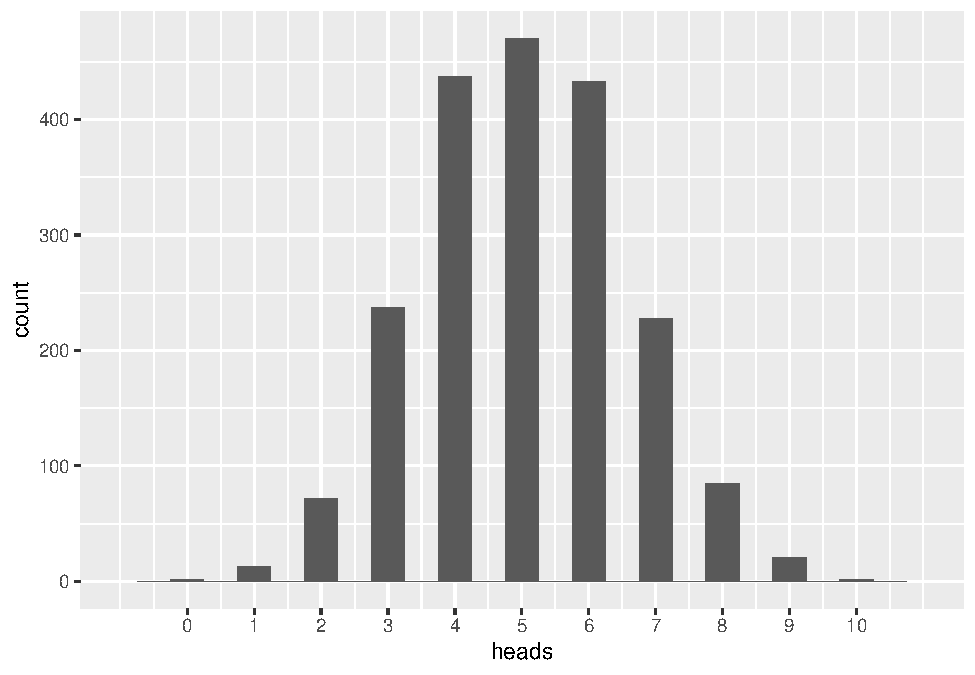
\includegraphics{intro_stats_files/figure-latex/unnamed-chunk-220-1.pdf}

This is helpful. In contrast with the set of simulations with twenty people, the last histogram gives us something closer to what we expect. The mode is at five heads, and every possible number of heads is represented, with decreasing counts as one moves away from five. With 2000 people flipping coins, all possible outcomes---including rare ones---are better represented.

Here is the the same histogram, but this time with the proportion of heads instead of the count of heads:

\begin{Shaded}
\begin{Highlighting}[]
\FunctionTok{ggplot}\NormalTok{(coin\_flips\_2000\_10, }\FunctionTok{aes}\NormalTok{(}\AttributeTok{x =}\NormalTok{ prop)) }\SpecialCharTok{+}
    \FunctionTok{geom\_histogram}\NormalTok{(}\AttributeTok{binwidth =} \FloatTok{0.05}\NormalTok{) }\SpecialCharTok{+}
    \FunctionTok{scale\_x\_continuous}\NormalTok{(}\AttributeTok{limits =} \FunctionTok{c}\NormalTok{(}\SpecialCharTok{{-}}\FloatTok{0.1}\NormalTok{, }\FloatTok{1.1}\NormalTok{), }\AttributeTok{breaks =} \FunctionTok{seq}\NormalTok{(}\DecValTok{0}\NormalTok{, }\DecValTok{1}\NormalTok{, }\FloatTok{0.1}\NormalTok{))}
\end{Highlighting}
\end{Shaded}

\begin{verbatim}
## Warning: Removed 2 rows containing missing values (geom_bar).
\end{verbatim}

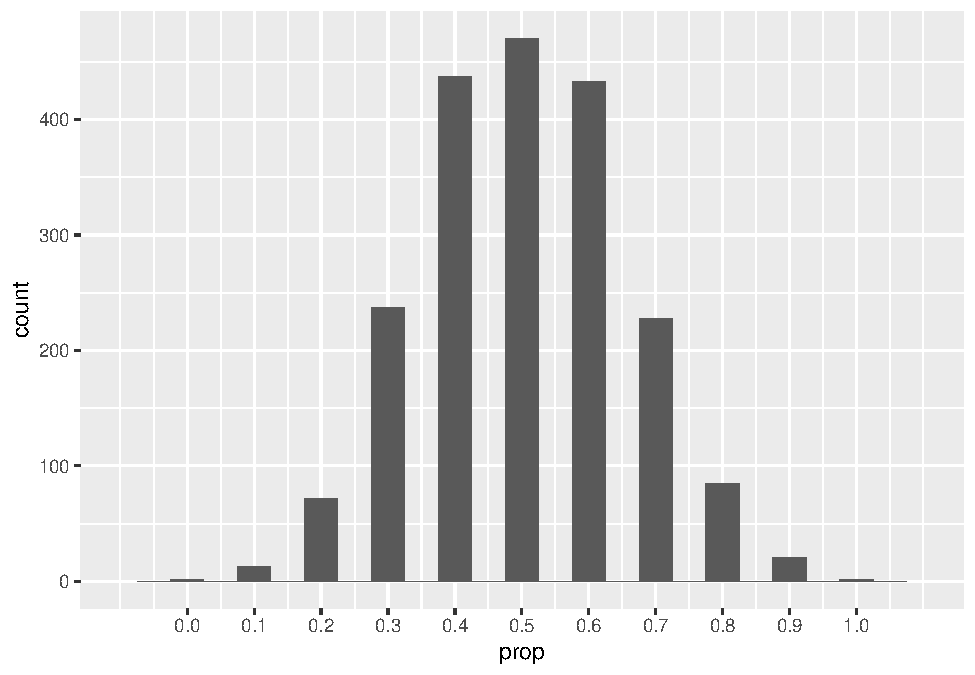
\includegraphics{intro_stats_files/figure-latex/unnamed-chunk-221-1.pdf}

\hypertarget{exercise-3-4}{%
\paragraph*{Exercise 3}\label{exercise-3-4}}
\addcontentsline{toc}{paragraph}{Exercise 3}

Do you think the shape of the distribution would be appreciably different if we used 20,000 or even 200,000 people? Why or why not? (Normally, I would encourage you to test your theory by trying it in R. However, it takes a \emph{long} time to simulate that many flips and I don't want you to tie up resources and memory. Think through this in your head.)

Please write up your answer here.

\begin{center}\rule{0.5\linewidth}{0.5pt}\end{center}

From now on, we will insist on using at least a thousand simulations---if not more---to make sure that we represent the full range of possible outcomes.\footnote{There is some theory behind choosing the number of times we need to simulate, but we're not going to get into all that.}

\hypertarget{randomization1-more}{%
\section{More flips}\label{randomization1-more}}

Now let's increase the number of coin flips each person performs. We'll still use 2000 simulations (imagine 2000 people all flipping coins), but this time, each person will flip the coin 1000 times instead of only 10 times. The first code chunk below accounts for a substantial amount of the time it takes to run the code in this document.

\begin{Shaded}
\begin{Highlighting}[]
\FunctionTok{set.seed}\NormalTok{(}\DecValTok{1234}\NormalTok{)}
\NormalTok{coin\_flips\_2000\_1000 }\OtherTok{\textless{}{-}} \FunctionTok{do}\NormalTok{(}\DecValTok{2000}\NormalTok{) }\SpecialCharTok{*} \FunctionTok{rflip}\NormalTok{(}\DecValTok{1000}\NormalTok{)}
\NormalTok{coin\_flips\_2000\_1000}
\end{Highlighting}
\end{Shaded}

\begin{verbatim}
##         n heads tails  prop
## 1    1000   485   515 0.485
## 2    1000   515   485 0.515
## 3    1000   481   519 0.481
## 4    1000   508   492 0.508
## 5    1000   499   501 0.499
## 6    1000   516   484 0.516
## 7    1000   497   503 0.497
## 8    1000   497   503 0.497
## 9    1000   494   506 0.494
## 10   1000   528   472 0.528
## 11   1000   495   505 0.495
## 12   1000   483   517 0.483
## 13   1000   520   480 0.520
## 14   1000   528   472 0.528
## 15   1000   478   522 0.478
## 16   1000   516   484 0.516
## 17   1000   493   507 0.493
## 18   1000   524   476 0.524
## 19   1000   473   527 0.473
## 20   1000   516   484 0.516
## 21   1000   529   471 0.529
## 22   1000   516   484 0.516
## 23   1000   535   465 0.535
## 24   1000   491   509 0.491
## 25   1000   500   500 0.500
## 26   1000   497   503 0.497
## 27   1000   507   493 0.507
## 28   1000   515   485 0.515
## 29   1000   493   507 0.493
## 30   1000   482   518 0.482
## 31   1000   485   515 0.485
## 32   1000   493   507 0.493
## 33   1000   498   502 0.498
## 34   1000   490   510 0.490
## 35   1000   485   515 0.485
## 36   1000   495   505 0.495
## 37   1000   488   512 0.488
## 38   1000   496   504 0.496
## 39   1000   491   509 0.491
## 40   1000   488   512 0.488
## 41   1000   488   512 0.488
## 42   1000   524   476 0.524
## 43   1000   500   500 0.500
## 44   1000   516   484 0.516
## 45   1000   514   486 0.514
## 46   1000   479   521 0.479
## 47   1000   488   512 0.488
## 48   1000   469   531 0.469
## 49   1000   515   485 0.515
## 50   1000   520   480 0.520
## 51   1000   486   514 0.486
## 52   1000   507   493 0.507
## 53   1000   509   491 0.509
## 54   1000   467   533 0.467
## 55   1000   467   533 0.467
## 56   1000   504   496 0.504
## 57   1000   483   517 0.483
## 58   1000   513   487 0.513
## 59   1000   518   482 0.518
## 60   1000   493   507 0.493
## 61   1000   516   484 0.516
## 62   1000   507   493 0.507
## 63   1000   509   491 0.509
## 64   1000   508   492 0.508
## 65   1000   511   489 0.511
## 66   1000   491   509 0.491
## 67   1000   524   476 0.524
## 68   1000   515   485 0.515
## 69   1000   524   476 0.524
## 70   1000   510   490 0.510
## 71   1000   482   518 0.482
## 72   1000   498   502 0.498
## 73   1000   507   493 0.507
## 74   1000   490   510 0.490
## 75   1000   501   499 0.501
## 76   1000   502   498 0.502
## 77   1000   520   480 0.520
## 78   1000   528   472 0.528
## 79   1000   504   496 0.504
## 80   1000   501   499 0.501
## 81   1000   507   493 0.507
## 82   1000   486   514 0.486
## 83   1000   500   500 0.500
## 84   1000   505   495 0.505
## 85   1000   494   506 0.494
## 86   1000   505   495 0.505
## 87   1000   512   488 0.512
## 88   1000   521   479 0.521
## 89   1000   497   503 0.497
## 90   1000   501   499 0.501
## 91   1000   489   511 0.489
## 92   1000   497   503 0.497
## 93   1000   500   500 0.500
## 94   1000   470   530 0.470
## 95   1000   511   489 0.511
## 96   1000   504   496 0.504
## 97   1000   460   540 0.460
## 98   1000   493   507 0.493
## 99   1000   477   523 0.477
## 100  1000   489   511 0.489
## 101  1000   511   489 0.511
## 102  1000   519   481 0.519
## 103  1000   491   509 0.491
## 104  1000   464   536 0.464
## 105  1000   493   507 0.493
## 106  1000   497   503 0.497
## 107  1000   515   485 0.515
## 108  1000   491   509 0.491
## 109  1000   472   528 0.472
## 110  1000   505   495 0.505
## 111  1000   503   497 0.503
## 112  1000   489   511 0.489
## 113  1000   530   470 0.530
## 114  1000   510   490 0.510
## 115  1000   521   479 0.521
## 116  1000   488   512 0.488
## 117  1000   453   547 0.453
## 118  1000   489   511 0.489
## 119  1000   486   514 0.486
## 120  1000   481   519 0.481
## 121  1000   495   505 0.495
## 122  1000   484   516 0.484
## 123  1000   534   466 0.534
## 124  1000   500   500 0.500
## 125  1000   497   503 0.497
## 126  1000   524   476 0.524
## 127  1000   494   506 0.494
## 128  1000   505   495 0.505
## 129  1000   479   521 0.479
## 130  1000   493   507 0.493
## 131  1000   488   512 0.488
## 132  1000   482   518 0.482
## 133  1000   519   481 0.519
## 134  1000   497   503 0.497
## 135  1000   531   469 0.531
## 136  1000   481   519 0.481
## 137  1000   510   490 0.510
## 138  1000   500   500 0.500
## 139  1000   476   524 0.476
## 140  1000   493   507 0.493
## 141  1000   490   510 0.490
## 142  1000   469   531 0.469
## 143  1000   484   516 0.484
## 144  1000   534   466 0.534
## 145  1000   491   509 0.491
## 146  1000   510   490 0.510
## 147  1000   507   493 0.507
## 148  1000   495   505 0.495
## 149  1000   526   474 0.526
## 150  1000   497   503 0.497
## 151  1000   510   490 0.510
## 152  1000   496   504 0.496
## 153  1000   470   530 0.470
## 154  1000   502   498 0.502
## 155  1000   485   515 0.485
## 156  1000   516   484 0.516
## 157  1000   513   487 0.513
## 158  1000   510   490 0.510
## 159  1000   484   516 0.484
## 160  1000   517   483 0.517
## 161  1000   512   488 0.512
## 162  1000   492   508 0.492
## 163  1000   513   487 0.513
## 164  1000   478   522 0.478
## 165  1000   503   497 0.503
## 166  1000   485   515 0.485
## 167  1000   489   511 0.489
## 168  1000   477   523 0.477
## 169  1000   508   492 0.508
## 170  1000   530   470 0.530
## 171  1000   476   524 0.476
## 172  1000   510   490 0.510
## 173  1000   475   525 0.475
## 174  1000   479   521 0.479
## 175  1000   497   503 0.497
## 176  1000   505   495 0.505
## 177  1000   506   494 0.506
## 178  1000   514   486 0.514
## 179  1000   511   489 0.511
## 180  1000   536   464 0.536
## 181  1000   487   513 0.487
## 182  1000   489   511 0.489
## 183  1000   487   513 0.487
## 184  1000   503   497 0.503
## 185  1000   493   507 0.493
## 186  1000   530   470 0.530
## 187  1000   496   504 0.496
## 188  1000   495   505 0.495
## 189  1000   481   519 0.481
## 190  1000   503   497 0.503
## 191  1000   482   518 0.482
## 192  1000   504   496 0.504
## 193  1000   513   487 0.513
## 194  1000   523   477 0.523
## 195  1000   512   488 0.512
## 196  1000   512   488 0.512
## 197  1000   508   492 0.508
## 198  1000   528   472 0.528
## 199  1000   498   502 0.498
## 200  1000   529   471 0.529
## 201  1000   516   484 0.516
## 202  1000   490   510 0.490
## 203  1000   498   502 0.498
## 204  1000   499   501 0.499
## 205  1000   502   498 0.502
## 206  1000   498   502 0.498
## 207  1000   503   497 0.503
## 208  1000   521   479 0.521
## 209  1000   509   491 0.509
## 210  1000   509   491 0.509
## 211  1000   492   508 0.492
## 212  1000   496   504 0.496
## 213  1000   516   484 0.516
## 214  1000   494   506 0.494
## 215  1000   487   513 0.487
## 216  1000   509   491 0.509
## 217  1000   487   513 0.487
## 218  1000   490   510 0.490
## 219  1000   520   480 0.520
## 220  1000   495   505 0.495
## 221  1000   500   500 0.500
## 222  1000   491   509 0.491
## 223  1000   511   489 0.511
## 224  1000   475   525 0.475
## 225  1000   515   485 0.515
## 226  1000   477   523 0.477
## 227  1000   501   499 0.501
## 228  1000   509   491 0.509
## 229  1000   490   510 0.490
## 230  1000   498   502 0.498
## 231  1000   494   506 0.494
## 232  1000   521   479 0.521
## 233  1000   477   523 0.477
## 234  1000   510   490 0.510
## 235  1000   517   483 0.517
## 236  1000   506   494 0.506
## 237  1000   477   523 0.477
## 238  1000   490   510 0.490
## 239  1000   524   476 0.524
## 240  1000   503   497 0.503
## 241  1000   514   486 0.514
## 242  1000   506   494 0.506
## 243  1000   482   518 0.482
## 244  1000   507   493 0.507
## 245  1000   504   496 0.504
## 246  1000   501   499 0.501
## 247  1000   482   518 0.482
## 248  1000   480   520 0.480
## 249  1000   511   489 0.511
## 250  1000   497   503 0.497
## 251  1000   471   529 0.471
## 252  1000   510   490 0.510
## 253  1000   523   477 0.523
## 254  1000   485   515 0.485
## 255  1000   505   495 0.505
## 256  1000   507   493 0.507
## 257  1000   473   527 0.473
## 258  1000   495   505 0.495
## 259  1000   465   535 0.465
## 260  1000   501   499 0.501
## 261  1000   460   540 0.460
## 262  1000   499   501 0.499
## 263  1000   524   476 0.524
## 264  1000   514   486 0.514
## 265  1000   503   497 0.503
## 266  1000   469   531 0.469
## 267  1000   496   504 0.496
## 268  1000   489   511 0.489
## 269  1000   507   493 0.507
## 270  1000   466   534 0.466
## 271  1000   482   518 0.482
## 272  1000   520   480 0.520
## 273  1000   513   487 0.513
## 274  1000   492   508 0.492
## 275  1000   486   514 0.486
## 276  1000   498   502 0.498
## 277  1000   507   493 0.507
## 278  1000   494   506 0.494
## 279  1000   499   501 0.499
## 280  1000   498   502 0.498
## 281  1000   459   541 0.459
## 282  1000   495   505 0.495
## 283  1000   498   502 0.498
## 284  1000   495   505 0.495
## 285  1000   488   512 0.488
## 286  1000   518   482 0.518
## 287  1000   502   498 0.502
## 288  1000   503   497 0.503
## 289  1000   476   524 0.476
## 290  1000   495   505 0.495
## 291  1000   495   505 0.495
## 292  1000   503   497 0.503
## 293  1000   482   518 0.482
## 294  1000   518   482 0.518
## 295  1000   514   486 0.514
## 296  1000   520   480 0.520
## 297  1000   498   502 0.498
## 298  1000   523   477 0.523
## 299  1000   516   484 0.516
## 300  1000   483   517 0.483
## 301  1000   504   496 0.504
## 302  1000   505   495 0.505
## 303  1000   502   498 0.502
## 304  1000   486   514 0.486
## 305  1000   540   460 0.540
## 306  1000   510   490 0.510
## 307  1000   507   493 0.507
## 308  1000   482   518 0.482
## 309  1000   509   491 0.509
## 310  1000   486   514 0.486
## 311  1000   474   526 0.474
## 312  1000   511   489 0.511
## 313  1000   484   516 0.484
## 314  1000   499   501 0.499
## 315  1000   496   504 0.496
## 316  1000   505   495 0.505
## 317  1000   487   513 0.487
## 318  1000   520   480 0.520
## 319  1000   483   517 0.483
## 320  1000   515   485 0.515
## 321  1000   513   487 0.513
## 322  1000   509   491 0.509
## 323  1000   520   480 0.520
## 324  1000   509   491 0.509
## 325  1000   480   520 0.480
## 326  1000   524   476 0.524
## 327  1000   507   493 0.507
## 328  1000   509   491 0.509
## 329  1000   493   507 0.493
## 330  1000   464   536 0.464
## 331  1000   526   474 0.526
## 332  1000   513   487 0.513
## 333  1000   505   495 0.505
## 334  1000   509   491 0.509
## 335  1000   500   500 0.500
## 336  1000   499   501 0.499
## 337  1000   520   480 0.520
## 338  1000   491   509 0.491
## 339  1000   488   512 0.488
## 340  1000   483   517 0.483
## 341  1000   508   492 0.508
## 342  1000   474   526 0.474
## 343  1000   482   518 0.482
## 344  1000   485   515 0.485
## 345  1000   516   484 0.516
## 346  1000   511   489 0.511
## 347  1000   490   510 0.490
## 348  1000   519   481 0.519
## 349  1000   493   507 0.493
## 350  1000   508   492 0.508
## 351  1000   492   508 0.492
## 352  1000   500   500 0.500
## 353  1000   503   497 0.503
## 354  1000   478   522 0.478
## 355  1000   511   489 0.511
## 356  1000   495   505 0.495
## 357  1000   472   528 0.472
## 358  1000   468   532 0.468
## 359  1000   504   496 0.504
## 360  1000   478   522 0.478
## 361  1000   485   515 0.485
## 362  1000   503   497 0.503
## 363  1000   487   513 0.487
## 364  1000   482   518 0.482
## 365  1000   485   515 0.485
## 366  1000   507   493 0.507
## 367  1000   477   523 0.477
## 368  1000   504   496 0.504
## 369  1000   502   498 0.502
## 370  1000   492   508 0.492
## 371  1000   485   515 0.485
## 372  1000   491   509 0.491
## 373  1000   502   498 0.502
## 374  1000   483   517 0.483
## 375  1000   510   490 0.510
## 376  1000   508   492 0.508
## 377  1000   500   500 0.500
## 378  1000   501   499 0.501
## 379  1000   518   482 0.518
## 380  1000   528   472 0.528
## 381  1000   500   500 0.500
## 382  1000   486   514 0.486
## 383  1000   487   513 0.487
## 384  1000   511   489 0.511
## 385  1000   483   517 0.483
## 386  1000   485   515 0.485
## 387  1000   485   515 0.485
## 388  1000   520   480 0.520
## 389  1000   486   514 0.486
## 390  1000   492   508 0.492
## 391  1000   519   481 0.519
## 392  1000   478   522 0.478
## 393  1000   509   491 0.509
## 394  1000   494   506 0.494
## 395  1000   482   518 0.482
## 396  1000   490   510 0.490
## 397  1000   488   512 0.488
## 398  1000   538   462 0.538
## 399  1000   483   517 0.483
## 400  1000   515   485 0.515
## 401  1000   489   511 0.489
## 402  1000   511   489 0.511
## 403  1000   486   514 0.486
## 404  1000   501   499 0.501
## 405  1000   497   503 0.497
## 406  1000   515   485 0.515
## 407  1000   514   486 0.514
## 408  1000   504   496 0.504
## 409  1000   526   474 0.526
## 410  1000   481   519 0.481
## 411  1000   505   495 0.505
## 412  1000   504   496 0.504
## 413  1000   511   489 0.511
## 414  1000   510   490 0.510
## 415  1000   494   506 0.494
## 416  1000   515   485 0.515
## 417  1000   510   490 0.510
## 418  1000   488   512 0.488
## 419  1000   490   510 0.490
## 420  1000   506   494 0.506
## 421  1000   489   511 0.489
## 422  1000   514   486 0.514
## 423  1000   524   476 0.524
## 424  1000   492   508 0.492
## 425  1000   502   498 0.502
## 426  1000   519   481 0.519
## 427  1000   500   500 0.500
## 428  1000   516   484 0.516
## 429  1000   515   485 0.515
## 430  1000   496   504 0.496
## 431  1000   479   521 0.479
## 432  1000   481   519 0.481
## 433  1000   521   479 0.521
## 434  1000   485   515 0.485
## 435  1000   492   508 0.492
## 436  1000   507   493 0.507
## 437  1000   507   493 0.507
## 438  1000   497   503 0.497
## 439  1000   516   484 0.516
## 440  1000   491   509 0.491
## 441  1000   518   482 0.518
## 442  1000   490   510 0.490
## 443  1000   502   498 0.502
## 444  1000   521   479 0.521
## 445  1000   504   496 0.504
## 446  1000   495   505 0.495
## 447  1000   500   500 0.500
## 448  1000   513   487 0.513
## 449  1000   497   503 0.497
## 450  1000   488   512 0.488
## 451  1000   497   503 0.497
## 452  1000   532   468 0.532
## 453  1000   519   481 0.519
## 454  1000   487   513 0.487
## 455  1000   500   500 0.500
## 456  1000   509   491 0.509
## 457  1000   506   494 0.506
## 458  1000   508   492 0.508
## 459  1000   524   476 0.524
## 460  1000   520   480 0.520
## 461  1000   509   491 0.509
## 462  1000   551   449 0.551
## 463  1000   512   488 0.512
## 464  1000   497   503 0.497
## 465  1000   500   500 0.500
## 466  1000   493   507 0.493
## 467  1000   508   492 0.508
## 468  1000   514   486 0.514
## 469  1000   524   476 0.524
## 470  1000   508   492 0.508
## 471  1000   493   507 0.493
## 472  1000   513   487 0.513
## 473  1000   515   485 0.515
## 474  1000   494   506 0.494
## 475  1000   487   513 0.487
## 476  1000   464   536 0.464
## 477  1000   511   489 0.511
## 478  1000   484   516 0.484
## 479  1000   527   473 0.527
## 480  1000   485   515 0.485
## 481  1000   495   505 0.495
## 482  1000   515   485 0.515
## 483  1000   484   516 0.484
## 484  1000   464   536 0.464
## 485  1000   541   459 0.541
## 486  1000   512   488 0.512
## 487  1000   506   494 0.506
## 488  1000   500   500 0.500
## 489  1000   522   478 0.522
## 490  1000   507   493 0.507
## 491  1000   521   479 0.521
## 492  1000   511   489 0.511
## 493  1000   486   514 0.486
## 494  1000   501   499 0.501
## 495  1000   515   485 0.515
## 496  1000   473   527 0.473
## 497  1000   499   501 0.499
## 498  1000   515   485 0.515
## 499  1000   519   481 0.519
## 500  1000   488   512 0.488
## 501  1000   508   492 0.508
## 502  1000   484   516 0.484
## 503  1000   484   516 0.484
## 504  1000   502   498 0.502
## 505  1000   489   511 0.489
## 506  1000   495   505 0.495
## 507  1000   519   481 0.519
## 508  1000   521   479 0.521
## 509  1000   506   494 0.506
## 510  1000   515   485 0.515
## 511  1000   499   501 0.499
## 512  1000   514   486 0.514
## 513  1000   527   473 0.527
## 514  1000   504   496 0.504
## 515  1000   469   531 0.469
## 516  1000   489   511 0.489
## 517  1000   503   497 0.503
## 518  1000   531   469 0.531
## 519  1000   497   503 0.497
## 520  1000   499   501 0.499
## 521  1000   483   517 0.483
## 522  1000   501   499 0.501
## 523  1000   481   519 0.481
## 524  1000   516   484 0.516
## 525  1000   491   509 0.491
## 526  1000   486   514 0.486
## 527  1000   492   508 0.492
## 528  1000   498   502 0.498
## 529  1000   522   478 0.522
## 530  1000   487   513 0.487
## 531  1000   477   523 0.477
## 532  1000   501   499 0.501
## 533  1000   490   510 0.490
## 534  1000   487   513 0.487
## 535  1000   490   510 0.490
## 536  1000   484   516 0.484
## 537  1000   489   511 0.489
## 538  1000   502   498 0.502
## 539  1000   490   510 0.490
## 540  1000   493   507 0.493
## 541  1000   509   491 0.509
## 542  1000   523   477 0.523
## 543  1000   501   499 0.501
## 544  1000   482   518 0.482
## 545  1000   498   502 0.498
## 546  1000   481   519 0.481
## 547  1000   502   498 0.502
## 548  1000   499   501 0.499
## 549  1000   504   496 0.504
## 550  1000   487   513 0.487
## 551  1000   481   519 0.481
## 552  1000   483   517 0.483
## 553  1000   488   512 0.488
## 554  1000   491   509 0.491
## 555  1000   532   468 0.532
## 556  1000   509   491 0.509
## 557  1000   495   505 0.495
## 558  1000   493   507 0.493
## 559  1000   519   481 0.519
## 560  1000   475   525 0.475
## 561  1000   523   477 0.523
## 562  1000   474   526 0.474
## 563  1000   461   539 0.461
## 564  1000   479   521 0.479
## 565  1000   528   472 0.528
## 566  1000   502   498 0.502
## 567  1000   503   497 0.503
## 568  1000   501   499 0.501
## 569  1000   487   513 0.487
## 570  1000   504   496 0.504
## 571  1000   504   496 0.504
## 572  1000   509   491 0.509
## 573  1000   493   507 0.493
## 574  1000   498   502 0.498
## 575  1000   488   512 0.488
## 576  1000   514   486 0.514
## 577  1000   482   518 0.482
## 578  1000   483   517 0.483
## 579  1000   500   500 0.500
## 580  1000   485   515 0.485
## 581  1000   503   497 0.503
## 582  1000   476   524 0.476
## 583  1000   518   482 0.518
## 584  1000   502   498 0.502
## 585  1000   496   504 0.496
## 586  1000   501   499 0.501
## 587  1000   501   499 0.501
## 588  1000   520   480 0.520
## 589  1000   489   511 0.489
## 590  1000   499   501 0.499
## 591  1000   484   516 0.484
## 592  1000   504   496 0.504
## 593  1000   510   490 0.510
## 594  1000   499   501 0.499
## 595  1000   490   510 0.490
## 596  1000   503   497 0.503
## 597  1000   486   514 0.486
## 598  1000   489   511 0.489
## 599  1000   505   495 0.505
## 600  1000   493   507 0.493
## 601  1000   490   510 0.490
## 602  1000   482   518 0.482
## 603  1000   522   478 0.522
## 604  1000   525   475 0.525
## 605  1000   503   497 0.503
## 606  1000   471   529 0.471
## 607  1000   501   499 0.501
## 608  1000   504   496 0.504
## 609  1000   495   505 0.495
## 610  1000   504   496 0.504
## 611  1000   494   506 0.494
## 612  1000   530   470 0.530
## 613  1000   484   516 0.484
## 614  1000   489   511 0.489
## 615  1000   500   500 0.500
## 616  1000   508   492 0.508
## 617  1000   492   508 0.492
## 618  1000   478   522 0.478
## 619  1000   534   466 0.534
## 620  1000   489   511 0.489
## 621  1000   503   497 0.503
## 622  1000   504   496 0.504
## 623  1000   484   516 0.484
## 624  1000   494   506 0.494
## 625  1000   483   517 0.483
## 626  1000   509   491 0.509
## 627  1000   520   480 0.520
## 628  1000   489   511 0.489
## 629  1000   501   499 0.501
## 630  1000   500   500 0.500
## 631  1000   483   517 0.483
## 632  1000   514   486 0.514
## 633  1000   513   487 0.513
## 634  1000   499   501 0.499
## 635  1000   492   508 0.492
## 636  1000   464   536 0.464
## 637  1000   508   492 0.508
## 638  1000   506   494 0.506
## 639  1000   499   501 0.499
## 640  1000   500   500 0.500
## 641  1000   512   488 0.512
## 642  1000   491   509 0.491
## 643  1000   510   490 0.510
## 644  1000   487   513 0.487
## 645  1000   484   516 0.484
## 646  1000   475   525 0.475
## 647  1000   501   499 0.501
## 648  1000   478   522 0.478
## 649  1000   490   510 0.490
## 650  1000   493   507 0.493
## 651  1000   510   490 0.510
## 652  1000   493   507 0.493
## 653  1000   519   481 0.519
## 654  1000   542   458 0.542
## 655  1000   495   505 0.495
## 656  1000   527   473 0.527
## 657  1000   537   463 0.537
## 658  1000   509   491 0.509
## 659  1000   461   539 0.461
## 660  1000   502   498 0.502
## 661  1000   508   492 0.508
## 662  1000   496   504 0.496
## 663  1000   487   513 0.487
## 664  1000   510   490 0.510
## 665  1000   488   512 0.488
## 666  1000   517   483 0.517
## 667  1000   503   497 0.503
## 668  1000   456   544 0.456
## 669  1000   470   530 0.470
## 670  1000   475   525 0.475
## 671  1000   510   490 0.510
## 672  1000   492   508 0.492
## 673  1000   492   508 0.492
## 674  1000   506   494 0.506
## 675  1000   492   508 0.492
## 676  1000   485   515 0.485
## 677  1000   500   500 0.500
## 678  1000   499   501 0.499
## 679  1000   512   488 0.512
## 680  1000   490   510 0.490
## 681  1000   502   498 0.502
## 682  1000   489   511 0.489
## 683  1000   499   501 0.499
## 684  1000   493   507 0.493
## 685  1000   494   506 0.494
## 686  1000   515   485 0.515
## 687  1000   488   512 0.488
## 688  1000   487   513 0.487
## 689  1000   504   496 0.504
## 690  1000   504   496 0.504
## 691  1000   481   519 0.481
## 692  1000   487   513 0.487
## 693  1000   512   488 0.512
## 694  1000   512   488 0.512
## 695  1000   474   526 0.474
## 696  1000   498   502 0.498
## 697  1000   504   496 0.504
## 698  1000   510   490 0.510
## 699  1000   501   499 0.501
## 700  1000   517   483 0.517
## 701  1000   507   493 0.507
## 702  1000   478   522 0.478
## 703  1000   536   464 0.536
## 704  1000   484   516 0.484
## 705  1000   482   518 0.482
## 706  1000   485   515 0.485
## 707  1000   510   490 0.510
## 708  1000   487   513 0.487
## 709  1000   484   516 0.484
## 710  1000   504   496 0.504
## 711  1000   499   501 0.499
## 712  1000   507   493 0.507
## 713  1000   490   510 0.490
## 714  1000   511   489 0.511
## 715  1000   521   479 0.521
## 716  1000   507   493 0.507
## 717  1000   504   496 0.504
## 718  1000   489   511 0.489
## 719  1000   487   513 0.487
## 720  1000   502   498 0.502
## 721  1000   502   498 0.502
## 722  1000   491   509 0.491
## 723  1000   484   516 0.484
## 724  1000   500   500 0.500
## 725  1000   512   488 0.512
## 726  1000   491   509 0.491
## 727  1000   496   504 0.496
## 728  1000   485   515 0.485
## 729  1000   523   477 0.523
## 730  1000   515   485 0.515
## 731  1000   503   497 0.503
## 732  1000   509   491 0.509
## 733  1000   487   513 0.487
## 734  1000   508   492 0.508
## 735  1000   480   520 0.480
## 736  1000   499   501 0.499
## 737  1000   495   505 0.495
## 738  1000   502   498 0.502
## 739  1000   516   484 0.516
## 740  1000   493   507 0.493
## 741  1000   484   516 0.484
## 742  1000   475   525 0.475
## 743  1000   483   517 0.483
## 744  1000   508   492 0.508
## 745  1000   523   477 0.523
## 746  1000   502   498 0.502
## 747  1000   503   497 0.503
## 748  1000   519   481 0.519
## 749  1000   483   517 0.483
## 750  1000   484   516 0.484
## 751  1000   501   499 0.501
## 752  1000   494   506 0.494
## 753  1000   511   489 0.511
## 754  1000   507   493 0.507
## 755  1000   493   507 0.493
## 756  1000   501   499 0.501
## 757  1000   507   493 0.507
## 758  1000   507   493 0.507
## 759  1000   522   478 0.522
## 760  1000   475   525 0.475
## 761  1000   501   499 0.501
## 762  1000   478   522 0.478
## 763  1000   504   496 0.504
## 764  1000   506   494 0.506
## 765  1000   499   501 0.499
## 766  1000   492   508 0.492
## 767  1000   503   497 0.503
## 768  1000   501   499 0.501
## 769  1000   512   488 0.512
## 770  1000   491   509 0.491
## 771  1000   503   497 0.503
## 772  1000   484   516 0.484
## 773  1000   525   475 0.525
## 774  1000   527   473 0.527
## 775  1000   514   486 0.514
## 776  1000   507   493 0.507
## 777  1000   485   515 0.485
## 778  1000   482   518 0.482
## 779  1000   502   498 0.502
## 780  1000   492   508 0.492
## 781  1000   494   506 0.494
## 782  1000   501   499 0.501
## 783  1000   492   508 0.492
## 784  1000   502   498 0.502
## 785  1000   516   484 0.516
## 786  1000   505   495 0.505
## 787  1000   497   503 0.497
## 788  1000   492   508 0.492
## 789  1000   497   503 0.497
## 790  1000   511   489 0.511
## 791  1000   499   501 0.499
## 792  1000   507   493 0.507
## 793  1000   493   507 0.493
## 794  1000   491   509 0.491
## 795  1000   480   520 0.480
## 796  1000   512   488 0.512
## 797  1000   520   480 0.520
## 798  1000   482   518 0.482
## 799  1000   511   489 0.511
## 800  1000   517   483 0.517
## 801  1000   497   503 0.497
## 802  1000   513   487 0.513
## 803  1000   502   498 0.502
## 804  1000   521   479 0.521
## 805  1000   505   495 0.505
## 806  1000   479   521 0.479
## 807  1000   508   492 0.508
## 808  1000   516   484 0.516
## 809  1000   500   500 0.500
## 810  1000   517   483 0.517
## 811  1000   479   521 0.479
## 812  1000   493   507 0.493
## 813  1000   507   493 0.507
## 814  1000   519   481 0.519
## 815  1000   496   504 0.496
## 816  1000   497   503 0.497
## 817  1000   498   502 0.498
## 818  1000   500   500 0.500
## 819  1000   507   493 0.507
## 820  1000   527   473 0.527
## 821  1000   463   537 0.463
## 822  1000   506   494 0.506
## 823  1000   511   489 0.511
## 824  1000   523   477 0.523
## 825  1000   515   485 0.515
## 826  1000   527   473 0.527
## 827  1000   519   481 0.519
## 828  1000   490   510 0.490
## 829  1000   505   495 0.505
## 830  1000   511   489 0.511
## 831  1000   469   531 0.469
## 832  1000   492   508 0.492
## 833  1000   497   503 0.497
## 834  1000   523   477 0.523
## 835  1000   480   520 0.480
## 836  1000   493   507 0.493
## 837  1000   529   471 0.529
## 838  1000   523   477 0.523
## 839  1000   499   501 0.499
## 840  1000   523   477 0.523
## 841  1000   501   499 0.501
## 842  1000   505   495 0.505
## 843  1000   523   477 0.523
## 844  1000   504   496 0.504
## 845  1000   492   508 0.492
## 846  1000   470   530 0.470
## 847  1000   493   507 0.493
## 848  1000   511   489 0.511
## 849  1000   485   515 0.485
## 850  1000   510   490 0.510
## 851  1000   498   502 0.498
## 852  1000   506   494 0.506
## 853  1000   501   499 0.501
## 854  1000   519   481 0.519
## 855  1000   514   486 0.514
## 856  1000   489   511 0.489
## 857  1000   513   487 0.513
## 858  1000   533   467 0.533
## 859  1000   485   515 0.485
## 860  1000   499   501 0.499
## 861  1000   490   510 0.490
## 862  1000   508   492 0.508
## 863  1000   482   518 0.482
## 864  1000   496   504 0.496
## 865  1000   496   504 0.496
## 866  1000   525   475 0.525
## 867  1000   500   500 0.500
## 868  1000   480   520 0.480
## 869  1000   493   507 0.493
## 870  1000   500   500 0.500
## 871  1000   489   511 0.489
## 872  1000   503   497 0.503
## 873  1000   479   521 0.479
## 874  1000   500   500 0.500
## 875  1000   499   501 0.499
## 876  1000   502   498 0.502
## 877  1000   485   515 0.485
## 878  1000   515   485 0.515
## 879  1000   512   488 0.512
## 880  1000   509   491 0.509
## 881  1000   499   501 0.499
## 882  1000   477   523 0.477
## 883  1000   515   485 0.515
## 884  1000   490   510 0.490
## 885  1000   505   495 0.505
## 886  1000   499   501 0.499
## 887  1000   495   505 0.495
## 888  1000   527   473 0.527
## 889  1000   514   486 0.514
## 890  1000   513   487 0.513
## 891  1000   505   495 0.505
## 892  1000   504   496 0.504
## 893  1000   482   518 0.482
## 894  1000   499   501 0.499
## 895  1000   491   509 0.491
## 896  1000   474   526 0.474
## 897  1000   513   487 0.513
## 898  1000   492   508 0.492
## 899  1000   504   496 0.504
## 900  1000   511   489 0.511
## 901  1000   488   512 0.488
## 902  1000   534   466 0.534
## 903  1000   485   515 0.485
## 904  1000   471   529 0.471
## 905  1000   511   489 0.511
## 906  1000   502   498 0.502
## 907  1000   517   483 0.517
## 908  1000   520   480 0.520
## 909  1000   525   475 0.525
## 910  1000   517   483 0.517
## 911  1000   495   505 0.495
## 912  1000   497   503 0.497
## 913  1000   493   507 0.493
## 914  1000   496   504 0.496
## 915  1000   472   528 0.472
## 916  1000   503   497 0.503
## 917  1000   512   488 0.512
## 918  1000   488   512 0.488
## 919  1000   482   518 0.482
## 920  1000   496   504 0.496
## 921  1000   474   526 0.474
## 922  1000   502   498 0.502
## 923  1000   490   510 0.490
## 924  1000   516   484 0.516
## 925  1000   488   512 0.488
## 926  1000   489   511 0.489
## 927  1000   477   523 0.477
## 928  1000   511   489 0.511
## 929  1000   486   514 0.486
## 930  1000   482   518 0.482
## 931  1000   486   514 0.486
## 932  1000   506   494 0.506
## 933  1000   492   508 0.492
## 934  1000   482   518 0.482
## 935  1000   509   491 0.509
## 936  1000   511   489 0.511
## 937  1000   477   523 0.477
## 938  1000   507   493 0.507
## 939  1000   506   494 0.506
## 940  1000   497   503 0.497
## 941  1000   506   494 0.506
## 942  1000   495   505 0.495
## 943  1000   513   487 0.513
## 944  1000   511   489 0.511
## 945  1000   486   514 0.486
## 946  1000   486   514 0.486
## 947  1000   511   489 0.511
## 948  1000   492   508 0.492
## 949  1000   475   525 0.475
## 950  1000   490   510 0.490
## 951  1000   488   512 0.488
## 952  1000   493   507 0.493
## 953  1000   485   515 0.485
## 954  1000   509   491 0.509
## 955  1000   486   514 0.486
## 956  1000   504   496 0.504
## 957  1000   477   523 0.477
## 958  1000   512   488 0.512
## 959  1000   501   499 0.501
## 960  1000   487   513 0.487
## 961  1000   493   507 0.493
## 962  1000   492   508 0.492
## 963  1000   512   488 0.512
## 964  1000   505   495 0.505
## 965  1000   494   506 0.494
## 966  1000   494   506 0.494
## 967  1000   493   507 0.493
## 968  1000   502   498 0.502
## 969  1000   498   502 0.498
## 970  1000   498   502 0.498
## 971  1000   517   483 0.517
## 972  1000   525   475 0.525
## 973  1000   530   470 0.530
## 974  1000   503   497 0.503
## 975  1000   486   514 0.486
## 976  1000   525   475 0.525
## 977  1000   503   497 0.503
## 978  1000   493   507 0.493
## 979  1000   485   515 0.485
## 980  1000   485   515 0.485
## 981  1000   529   471 0.529
## 982  1000   508   492 0.508
## 983  1000   495   505 0.495
## 984  1000   488   512 0.488
## 985  1000   519   481 0.519
## 986  1000   515   485 0.515
## 987  1000   464   536 0.464
## 988  1000   524   476 0.524
## 989  1000   522   478 0.522
## 990  1000   520   480 0.520
## 991  1000   508   492 0.508
## 992  1000   512   488 0.512
## 993  1000   504   496 0.504
## 994  1000   481   519 0.481
## 995  1000   450   550 0.450
## 996  1000   500   500 0.500
## 997  1000   499   501 0.499
## 998  1000   487   513 0.487
## 999  1000   481   519 0.481
## 1000 1000   498   502 0.498
## 1001 1000   520   480 0.520
## 1002 1000   492   508 0.492
## 1003 1000   532   468 0.532
## 1004 1000   512   488 0.512
## 1005 1000   503   497 0.503
## 1006 1000   482   518 0.482
## 1007 1000   486   514 0.486
## 1008 1000   518   482 0.518
## 1009 1000   469   531 0.469
## 1010 1000   468   532 0.468
## 1011 1000   471   529 0.471
## 1012 1000   524   476 0.524
## 1013 1000   500   500 0.500
## 1014 1000   514   486 0.514
## 1015 1000   510   490 0.510
## 1016 1000   478   522 0.478
## 1017 1000   518   482 0.518
## 1018 1000   503   497 0.503
## 1019 1000   512   488 0.512
## 1020 1000   506   494 0.506
## 1021 1000   492   508 0.492
## 1022 1000   513   487 0.513
## 1023 1000   499   501 0.499
## 1024 1000   469   531 0.469
## 1025 1000   497   503 0.497
## 1026 1000   491   509 0.491
## 1027 1000   508   492 0.508
## 1028 1000   498   502 0.498
## 1029 1000   500   500 0.500
## 1030 1000   513   487 0.513
## 1031 1000   502   498 0.502
## 1032 1000   528   472 0.528
## 1033 1000   482   518 0.482
## 1034 1000   497   503 0.497
## 1035 1000   510   490 0.510
## 1036 1000   509   491 0.509
## 1037 1000   490   510 0.490
## 1038 1000   500   500 0.500
## 1039 1000   470   530 0.470
## 1040 1000   481   519 0.481
## 1041 1000   510   490 0.510
## 1042 1000   465   535 0.465
## 1043 1000   501   499 0.501
## 1044 1000   495   505 0.495
## 1045 1000   490   510 0.490
## 1046 1000   491   509 0.491
## 1047 1000   497   503 0.497
## 1048 1000   495   505 0.495
## 1049 1000   532   468 0.532
## 1050 1000   497   503 0.497
## 1051 1000   510   490 0.510
## 1052 1000   488   512 0.488
## 1053 1000   480   520 0.480
## 1054 1000   532   468 0.532
## 1055 1000   484   516 0.484
## 1056 1000   512   488 0.512
## 1057 1000   491   509 0.491
## 1058 1000   498   502 0.498
## 1059 1000   495   505 0.495
## 1060 1000   482   518 0.482
## 1061 1000   495   505 0.495
## 1062 1000   489   511 0.489
## 1063 1000   486   514 0.486
## 1064 1000   515   485 0.515
## 1065 1000   500   500 0.500
## 1066 1000   494   506 0.494
## 1067 1000   520   480 0.520
## 1068 1000   516   484 0.516
## 1069 1000   497   503 0.497
## 1070 1000   511   489 0.511
## 1071 1000   499   501 0.499
## 1072 1000   475   525 0.475
## 1073 1000   480   520 0.480
## 1074 1000   508   492 0.508
## 1075 1000   487   513 0.487
## 1076 1000   483   517 0.483
## 1077 1000   500   500 0.500
## 1078 1000   502   498 0.502
## 1079 1000   471   529 0.471
## 1080 1000   526   474 0.526
## 1081 1000   494   506 0.494
## 1082 1000   507   493 0.507
## 1083 1000   508   492 0.508
## 1084 1000   487   513 0.487
## 1085 1000   493   507 0.493
## 1086 1000   504   496 0.504
## 1087 1000   514   486 0.514
## 1088 1000   512   488 0.512
## 1089 1000   499   501 0.499
## 1090 1000   531   469 0.531
## 1091 1000   485   515 0.485
## 1092 1000   515   485 0.515
## 1093 1000   475   525 0.475
## 1094 1000   473   527 0.473
## 1095 1000   487   513 0.487
## 1096 1000   481   519 0.481
## 1097 1000   486   514 0.486
## 1098 1000   466   534 0.466
## 1099 1000   475   525 0.475
## 1100 1000   513   487 0.513
## 1101 1000   497   503 0.497
## 1102 1000   523   477 0.523
## 1103 1000   491   509 0.491
## 1104 1000   521   479 0.521
## 1105 1000   489   511 0.489
## 1106 1000   512   488 0.512
## 1107 1000   496   504 0.496
## 1108 1000   517   483 0.517
## 1109 1000   533   467 0.533
## 1110 1000   527   473 0.527
## 1111 1000   533   467 0.533
## 1112 1000   497   503 0.497
## 1113 1000   490   510 0.490
## 1114 1000   481   519 0.481
## 1115 1000   491   509 0.491
## 1116 1000   489   511 0.489
## 1117 1000   472   528 0.472
## 1118 1000   511   489 0.511
## 1119 1000   494   506 0.494
## 1120 1000   545   455 0.545
## 1121 1000   498   502 0.498
## 1122 1000   490   510 0.490
## 1123 1000   516   484 0.516
## 1124 1000   475   525 0.475
## 1125 1000   494   506 0.494
## 1126 1000   537   463 0.537
## 1127 1000   481   519 0.481
## 1128 1000   495   505 0.495
## 1129 1000   488   512 0.488
## 1130 1000   490   510 0.490
## 1131 1000   486   514 0.486
## 1132 1000   527   473 0.527
## 1133 1000   501   499 0.501
## 1134 1000   505   495 0.505
## 1135 1000   502   498 0.502
## 1136 1000   494   506 0.494
## 1137 1000   495   505 0.495
## 1138 1000   517   483 0.517
## 1139 1000   480   520 0.480
## 1140 1000   477   523 0.477
## 1141 1000   505   495 0.505
## 1142 1000   516   484 0.516
## 1143 1000   526   474 0.526
## 1144 1000   518   482 0.518
## 1145 1000   495   505 0.495
## 1146 1000   511   489 0.511
## 1147 1000   493   507 0.493
## 1148 1000   506   494 0.506
## 1149 1000   498   502 0.498
## 1150 1000   504   496 0.504
## 1151 1000   509   491 0.509
## 1152 1000   487   513 0.487
## 1153 1000   504   496 0.504
## 1154 1000   496   504 0.496
## 1155 1000   512   488 0.512
## 1156 1000   477   523 0.477
## 1157 1000   514   486 0.514
## 1158 1000   511   489 0.511
## 1159 1000   475   525 0.475
## 1160 1000   464   536 0.464
## 1161 1000   448   552 0.448
## 1162 1000   526   474 0.526
## 1163 1000   538   462 0.538
## 1164 1000   499   501 0.499
## 1165 1000   487   513 0.487
## 1166 1000   509   491 0.509
## 1167 1000   501   499 0.501
## 1168 1000   481   519 0.481
## 1169 1000   509   491 0.509
## 1170 1000   486   514 0.486
## 1171 1000   487   513 0.487
## 1172 1000   491   509 0.491
## 1173 1000   489   511 0.489
## 1174 1000   475   525 0.475
## 1175 1000   474   526 0.474
## 1176 1000   473   527 0.473
## 1177 1000   513   487 0.513
## 1178 1000   517   483 0.517
## 1179 1000   497   503 0.497
## 1180 1000   469   531 0.469
## 1181 1000   520   480 0.520
## 1182 1000   457   543 0.457
## 1183 1000   532   468 0.532
## 1184 1000   500   500 0.500
## 1185 1000   514   486 0.514
## 1186 1000   522   478 0.522
## 1187 1000   517   483 0.517
## 1188 1000   518   482 0.518
## 1189 1000   503   497 0.503
## 1190 1000   506   494 0.506
## 1191 1000   504   496 0.504
## 1192 1000   509   491 0.509
## 1193 1000   506   494 0.506
## 1194 1000   511   489 0.511
## 1195 1000   496   504 0.496
## 1196 1000   513   487 0.513
## 1197 1000   505   495 0.505
## 1198 1000   512   488 0.512
## 1199 1000   495   505 0.495
## 1200 1000   512   488 0.512
## 1201 1000   495   505 0.495
## 1202 1000   527   473 0.527
## 1203 1000   495   505 0.495
## 1204 1000   513   487 0.513
## 1205 1000   515   485 0.515
## 1206 1000   488   512 0.488
## 1207 1000   495   505 0.495
## 1208 1000   494   506 0.494
## 1209 1000   505   495 0.505
## 1210 1000   500   500 0.500
## 1211 1000   483   517 0.483
## 1212 1000   505   495 0.505
## 1213 1000   523   477 0.523
## 1214 1000   508   492 0.508
## 1215 1000   498   502 0.498
## 1216 1000   499   501 0.499
## 1217 1000   489   511 0.489
## 1218 1000   505   495 0.505
## 1219 1000   509   491 0.509
## 1220 1000   501   499 0.501
## 1221 1000   496   504 0.496
## 1222 1000   496   504 0.496
## 1223 1000   504   496 0.504
## 1224 1000   491   509 0.491
## 1225 1000   500   500 0.500
## 1226 1000   523   477 0.523
## 1227 1000   499   501 0.499
## 1228 1000   489   511 0.489
## 1229 1000   486   514 0.486
## 1230 1000   515   485 0.515
## 1231 1000   494   506 0.494
## 1232 1000   496   504 0.496
## 1233 1000   496   504 0.496
## 1234 1000   486   514 0.486
## 1235 1000   533   467 0.533
## 1236 1000   487   513 0.487
## 1237 1000   485   515 0.485
## 1238 1000   503   497 0.503
## 1239 1000   508   492 0.508
## 1240 1000   510   490 0.510
## 1241 1000   496   504 0.496
## 1242 1000   497   503 0.497
## 1243 1000   504   496 0.504
## 1244 1000   470   530 0.470
## 1245 1000   512   488 0.512
## 1246 1000   526   474 0.526
## 1247 1000   487   513 0.487
## 1248 1000   508   492 0.508
## 1249 1000   505   495 0.505
## 1250 1000   519   481 0.519
## 1251 1000   490   510 0.490
## 1252 1000   475   525 0.475
## 1253 1000   479   521 0.479
## 1254 1000   509   491 0.509
## 1255 1000   500   500 0.500
## 1256 1000   479   521 0.479
## 1257 1000   529   471 0.529
## 1258 1000   518   482 0.518
## 1259 1000   510   490 0.510
## 1260 1000   482   518 0.482
## 1261 1000   498   502 0.498
## 1262 1000   478   522 0.478
## 1263 1000   498   502 0.498
## 1264 1000   521   479 0.521
## 1265 1000   501   499 0.501
## 1266 1000   489   511 0.489
## 1267 1000   502   498 0.502
## 1268 1000   509   491 0.509
## 1269 1000   502   498 0.502
## 1270 1000   455   545 0.455
## 1271 1000   486   514 0.486
## 1272 1000   524   476 0.524
## 1273 1000   510   490 0.510
## 1274 1000   492   508 0.492
## 1275 1000   484   516 0.484
## 1276 1000   480   520 0.480
## 1277 1000   520   480 0.520
## 1278 1000   486   514 0.486
## 1279 1000   506   494 0.506
## 1280 1000   492   508 0.492
## 1281 1000   512   488 0.512
## 1282 1000   522   478 0.522
## 1283 1000   525   475 0.525
## 1284 1000   494   506 0.494
## 1285 1000   500   500 0.500
## 1286 1000   499   501 0.499
## 1287 1000   522   478 0.522
## 1288 1000   494   506 0.494
## 1289 1000   525   475 0.525
## 1290 1000   506   494 0.506
## 1291 1000   496   504 0.496
## 1292 1000   524   476 0.524
## 1293 1000   475   525 0.475
## 1294 1000   465   535 0.465
## 1295 1000   495   505 0.495
## 1296 1000   517   483 0.517
## 1297 1000   502   498 0.502
## 1298 1000   494   506 0.494
## 1299 1000   518   482 0.518
## 1300 1000   479   521 0.479
## 1301 1000   513   487 0.513
## 1302 1000   522   478 0.522
## 1303 1000   494   506 0.494
## 1304 1000   499   501 0.499
## 1305 1000   493   507 0.493
## 1306 1000   535   465 0.535
## 1307 1000   495   505 0.495
## 1308 1000   507   493 0.507
## 1309 1000   509   491 0.509
## 1310 1000   500   500 0.500
## 1311 1000   480   520 0.480
## 1312 1000   524   476 0.524
## 1313 1000   489   511 0.489
## 1314 1000   504   496 0.504
## 1315 1000   516   484 0.516
## 1316 1000   521   479 0.521
## 1317 1000   532   468 0.532
## 1318 1000   518   482 0.518
## 1319 1000   500   500 0.500
## 1320 1000   502   498 0.502
## 1321 1000   491   509 0.491
## 1322 1000   529   471 0.529
## 1323 1000   513   487 0.513
## 1324 1000   489   511 0.489
## 1325 1000   496   504 0.496
## 1326 1000   515   485 0.515
## 1327 1000   498   502 0.498
## 1328 1000   495   505 0.495
## 1329 1000   459   541 0.459
## 1330 1000   521   479 0.521
## 1331 1000   515   485 0.515
## 1332 1000   491   509 0.491
## 1333 1000   496   504 0.496
## 1334 1000   514   486 0.514
## 1335 1000   497   503 0.497
## 1336 1000   515   485 0.515
## 1337 1000   483   517 0.483
## 1338 1000   497   503 0.497
## 1339 1000   496   504 0.496
## 1340 1000   495   505 0.495
## 1341 1000   497   503 0.497
## 1342 1000   499   501 0.499
## 1343 1000   515   485 0.515
## 1344 1000   520   480 0.520
## 1345 1000   520   480 0.520
## 1346 1000   513   487 0.513
## 1347 1000   504   496 0.504
## 1348 1000   528   472 0.528
## 1349 1000   489   511 0.489
## 1350 1000   512   488 0.512
## 1351 1000   527   473 0.527
## 1352 1000   503   497 0.503
## 1353 1000   471   529 0.471
## 1354 1000   478   522 0.478
## 1355 1000   501   499 0.501
## 1356 1000   491   509 0.491
## 1357 1000   504   496 0.504
## 1358 1000   502   498 0.502
## 1359 1000   471   529 0.471
## 1360 1000   492   508 0.492
## 1361 1000   488   512 0.488
## 1362 1000   494   506 0.494
## 1363 1000   531   469 0.531
## 1364 1000   473   527 0.473
## 1365 1000   487   513 0.487
## 1366 1000   503   497 0.503
## 1367 1000   494   506 0.494
## 1368 1000   530   470 0.530
## 1369 1000   496   504 0.496
## 1370 1000   517   483 0.517
## 1371 1000   526   474 0.526
## 1372 1000   515   485 0.515
## 1373 1000   488   512 0.488
## 1374 1000   455   545 0.455
## 1375 1000   503   497 0.503
## 1376 1000   494   506 0.494
## 1377 1000   527   473 0.527
## 1378 1000   503   497 0.503
## 1379 1000   472   528 0.472
## 1380 1000   511   489 0.511
## 1381 1000   488   512 0.488
## 1382 1000   493   507 0.493
## 1383 1000   520   480 0.520
## 1384 1000   524   476 0.524
## 1385 1000   508   492 0.508
## 1386 1000   515   485 0.515
## 1387 1000   519   481 0.519
## 1388 1000   490   510 0.490
## 1389 1000   477   523 0.477
## 1390 1000   508   492 0.508
## 1391 1000   515   485 0.515
## 1392 1000   520   480 0.520
## 1393 1000   489   511 0.489
## 1394 1000   500   500 0.500
## 1395 1000   519   481 0.519
## 1396 1000   493   507 0.493
## 1397 1000   509   491 0.509
## 1398 1000   489   511 0.489
## 1399 1000   494   506 0.494
## 1400 1000   508   492 0.508
## 1401 1000   513   487 0.513
## 1402 1000   514   486 0.514
## 1403 1000   516   484 0.516
## 1404 1000   502   498 0.502
## 1405 1000   496   504 0.496
## 1406 1000   483   517 0.483
## 1407 1000   516   484 0.516
## 1408 1000   502   498 0.502
## 1409 1000   510   490 0.510
## 1410 1000   469   531 0.469
## 1411 1000   487   513 0.487
## 1412 1000   518   482 0.518
## 1413 1000   499   501 0.499
## 1414 1000   463   537 0.463
## 1415 1000   521   479 0.521
## 1416 1000   483   517 0.483
## 1417 1000   469   531 0.469
## 1418 1000   493   507 0.493
## 1419 1000   496   504 0.496
## 1420 1000   482   518 0.482
## 1421 1000   477   523 0.477
## 1422 1000   536   464 0.536
## 1423 1000   507   493 0.507
## 1424 1000   505   495 0.505
## 1425 1000   511   489 0.511
## 1426 1000   517   483 0.517
## 1427 1000   510   490 0.510
## 1428 1000   486   514 0.486
## 1429 1000   520   480 0.520
## 1430 1000   493   507 0.493
## 1431 1000   497   503 0.497
## 1432 1000   491   509 0.491
## 1433 1000   520   480 0.520
## 1434 1000   494   506 0.494
## 1435 1000   514   486 0.514
## 1436 1000   479   521 0.479
## 1437 1000   506   494 0.506
## 1438 1000   492   508 0.492
## 1439 1000   474   526 0.474
## 1440 1000   501   499 0.501
## 1441 1000   504   496 0.504
## 1442 1000   507   493 0.507
## 1443 1000   482   518 0.482
## 1444 1000   512   488 0.512
## 1445 1000   506   494 0.506
## 1446 1000   516   484 0.516
## 1447 1000   504   496 0.504
## 1448 1000   508   492 0.508
## 1449 1000   504   496 0.504
## 1450 1000   499   501 0.499
## 1451 1000   520   480 0.520
## 1452 1000   484   516 0.484
## 1453 1000   504   496 0.504
## 1454 1000   499   501 0.499
## 1455 1000   499   501 0.499
## 1456 1000   500   500 0.500
## 1457 1000   503   497 0.503
## 1458 1000   488   512 0.488
## 1459 1000   474   526 0.474
## 1460 1000   504   496 0.504
## 1461 1000   510   490 0.510
## 1462 1000   498   502 0.498
## 1463 1000   510   490 0.510
## 1464 1000   523   477 0.523
## 1465 1000   525   475 0.525
## 1466 1000   475   525 0.475
## 1467 1000   496   504 0.496
## 1468 1000   482   518 0.482
## 1469 1000   506   494 0.506
## 1470 1000   468   532 0.468
## 1471 1000   500   500 0.500
## 1472 1000   486   514 0.486
## 1473 1000   508   492 0.508
## 1474 1000   517   483 0.517
## 1475 1000   507   493 0.507
## 1476 1000   518   482 0.518
## 1477 1000   508   492 0.508
## 1478 1000   482   518 0.482
## 1479 1000   504   496 0.504
## 1480 1000   483   517 0.483
## 1481 1000   521   479 0.521
## 1482 1000   506   494 0.506
## 1483 1000   510   490 0.510
## 1484 1000   500   500 0.500
## 1485 1000   473   527 0.473
## 1486 1000   516   484 0.516
## 1487 1000   505   495 0.505
## 1488 1000   486   514 0.486
## 1489 1000   467   533 0.467
## 1490 1000   522   478 0.522
## 1491 1000   515   485 0.515
## 1492 1000   495   505 0.495
## 1493 1000   476   524 0.476
## 1494 1000   497   503 0.497
## 1495 1000   514   486 0.514
## 1496 1000   490   510 0.490
## 1497 1000   518   482 0.518
## 1498 1000   508   492 0.508
## 1499 1000   480   520 0.480
## 1500 1000   501   499 0.501
## 1501 1000   490   510 0.490
## 1502 1000   475   525 0.475
## 1503 1000   493   507 0.493
## 1504 1000   498   502 0.498
## 1505 1000   541   459 0.541
## 1506 1000   484   516 0.484
## 1507 1000   508   492 0.508
## 1508 1000   453   547 0.453
## 1509 1000   530   470 0.530
## 1510 1000   491   509 0.491
## 1511 1000   496   504 0.496
## 1512 1000   520   480 0.520
## 1513 1000   508   492 0.508
## 1514 1000   504   496 0.504
## 1515 1000   524   476 0.524
## 1516 1000   510   490 0.510
## 1517 1000   500   500 0.500
## 1518 1000   490   510 0.490
## 1519 1000   505   495 0.505
## 1520 1000   509   491 0.509
## 1521 1000   525   475 0.525
## 1522 1000   493   507 0.493
## 1523 1000   511   489 0.511
## 1524 1000   497   503 0.497
## 1525 1000   479   521 0.479
## 1526 1000   489   511 0.489
## 1527 1000   528   472 0.528
## 1528 1000   515   485 0.515
## 1529 1000   492   508 0.492
## 1530 1000   498   502 0.498
## 1531 1000   518   482 0.518
## 1532 1000   484   516 0.484
## 1533 1000   485   515 0.485
## 1534 1000   502   498 0.502
## 1535 1000   515   485 0.515
## 1536 1000   535   465 0.535
## 1537 1000   529   471 0.529
## 1538 1000   481   519 0.481
## 1539 1000   505   495 0.505
## 1540 1000   492   508 0.492
## 1541 1000   478   522 0.478
## 1542 1000   514   486 0.514
## 1543 1000   491   509 0.491
## 1544 1000   494   506 0.494
## 1545 1000   498   502 0.498
## 1546 1000   487   513 0.487
## 1547 1000   494   506 0.494
## 1548 1000   511   489 0.511
## 1549 1000   510   490 0.510
## 1550 1000   488   512 0.488
## 1551 1000   491   509 0.491
## 1552 1000   544   456 0.544
## 1553 1000   514   486 0.514
## 1554 1000   501   499 0.501
## 1555 1000   506   494 0.506
## 1556 1000   485   515 0.485
## 1557 1000   505   495 0.505
## 1558 1000   490   510 0.490
## 1559 1000   502   498 0.502
## 1560 1000   500   500 0.500
## 1561 1000   485   515 0.485
## 1562 1000   503   497 0.503
## 1563 1000   483   517 0.483
## 1564 1000   517   483 0.517
## 1565 1000   509   491 0.509
## 1566 1000   510   490 0.510
## 1567 1000   488   512 0.488
## 1568 1000   491   509 0.491
## 1569 1000   526   474 0.526
## 1570 1000   484   516 0.484
## 1571 1000   494   506 0.494
## 1572 1000   498   502 0.498
## 1573 1000   481   519 0.481
## 1574 1000   520   480 0.520
## 1575 1000   504   496 0.504
## 1576 1000   512   488 0.512
## 1577 1000   510   490 0.510
## 1578 1000   503   497 0.503
## 1579 1000   501   499 0.501
## 1580 1000   495   505 0.495
## 1581 1000   497   503 0.497
## 1582 1000   533   467 0.533
## 1583 1000   521   479 0.521
## 1584 1000   492   508 0.492
## 1585 1000   496   504 0.496
## 1586 1000   484   516 0.484
## 1587 1000   487   513 0.487
## 1588 1000   495   505 0.495
## 1589 1000   476   524 0.476
## 1590 1000   483   517 0.483
## 1591 1000   520   480 0.520
## 1592 1000   502   498 0.502
## 1593 1000   497   503 0.497
## 1594 1000   495   505 0.495
## 1595 1000   510   490 0.510
## 1596 1000   500   500 0.500
## 1597 1000   517   483 0.517
## 1598 1000   513   487 0.513
## 1599 1000   491   509 0.491
## 1600 1000   475   525 0.475
## 1601 1000   498   502 0.498
## 1602 1000   516   484 0.516
## 1603 1000   493   507 0.493
## 1604 1000   485   515 0.485
## 1605 1000   504   496 0.504
## 1606 1000   496   504 0.496
## 1607 1000   480   520 0.480
## 1608 1000   498   502 0.498
## 1609 1000   530   470 0.530
## 1610 1000   470   530 0.470
## 1611 1000   516   484 0.516
## 1612 1000   514   486 0.514
## 1613 1000   500   500 0.500
## 1614 1000   469   531 0.469
## 1615 1000   495   505 0.495
## 1616 1000   489   511 0.489
## 1617 1000   503   497 0.503
## 1618 1000   475   525 0.475
## 1619 1000   492   508 0.492
## 1620 1000   504   496 0.504
## 1621 1000   488   512 0.488
## 1622 1000   492   508 0.492
## 1623 1000   516   484 0.516
## 1624 1000   479   521 0.479
## 1625 1000   502   498 0.502
## 1626 1000   490   510 0.490
## 1627 1000   493   507 0.493
## 1628 1000   517   483 0.517
## 1629 1000   509   491 0.509
## 1630 1000   498   502 0.498
## 1631 1000   517   483 0.517
## 1632 1000   497   503 0.497
## 1633 1000   519   481 0.519
## 1634 1000   493   507 0.493
## 1635 1000   500   500 0.500
## 1636 1000   501   499 0.501
## 1637 1000   486   514 0.486
## 1638 1000   502   498 0.502
## 1639 1000   500   500 0.500
## 1640 1000   505   495 0.505
## 1641 1000   464   536 0.464
## 1642 1000   500   500 0.500
## 1643 1000   502   498 0.502
## 1644 1000   488   512 0.488
## 1645 1000   480   520 0.480
## 1646 1000   491   509 0.491
## 1647 1000   529   471 0.529
## 1648 1000   490   510 0.490
## 1649 1000   487   513 0.487
## 1650 1000   494   506 0.494
## 1651 1000   527   473 0.527
## 1652 1000   493   507 0.493
## 1653 1000   512   488 0.512
## 1654 1000   512   488 0.512
## 1655 1000   481   519 0.481
## 1656 1000   486   514 0.486
## 1657 1000   459   541 0.459
## 1658 1000   487   513 0.487
## 1659 1000   481   519 0.481
## 1660 1000   544   456 0.544
## 1661 1000   479   521 0.479
## 1662 1000   513   487 0.513
## 1663 1000   501   499 0.501
## 1664 1000   480   520 0.480
## 1665 1000   489   511 0.489
## 1666 1000   491   509 0.491
## 1667 1000   503   497 0.503
## 1668 1000   527   473 0.527
## 1669 1000   506   494 0.506
## 1670 1000   487   513 0.487
## 1671 1000   506   494 0.506
## 1672 1000   506   494 0.506
## 1673 1000   485   515 0.485
## 1674 1000   525   475 0.525
## 1675 1000   520   480 0.520
## 1676 1000   490   510 0.490
## 1677 1000   508   492 0.508
## 1678 1000   488   512 0.488
## 1679 1000   505   495 0.505
## 1680 1000   485   515 0.485
## 1681 1000   508   492 0.508
## 1682 1000   473   527 0.473
## 1683 1000   503   497 0.503
## 1684 1000   526   474 0.526
## 1685 1000   496   504 0.496
## 1686 1000   524   476 0.524
## 1687 1000   498   502 0.498
## 1688 1000   540   460 0.540
## 1689 1000   486   514 0.486
## 1690 1000   491   509 0.491
## 1691 1000   499   501 0.499
## 1692 1000   521   479 0.521
## 1693 1000   496   504 0.496
## 1694 1000   501   499 0.501
## 1695 1000   485   515 0.485
## 1696 1000   482   518 0.482
## 1697 1000   510   490 0.510
## 1698 1000   488   512 0.488
## 1699 1000   499   501 0.499
## 1700 1000   486   514 0.486
## 1701 1000   496   504 0.496
## 1702 1000   504   496 0.504
## 1703 1000   499   501 0.499
## 1704 1000   484   516 0.484
## 1705 1000   489   511 0.489
## 1706 1000   491   509 0.491
## 1707 1000   515   485 0.515
## 1708 1000   476   524 0.476
## 1709 1000   508   492 0.508
## 1710 1000   485   515 0.485
## 1711 1000   483   517 0.483
## 1712 1000   529   471 0.529
## 1713 1000   552   448 0.552
## 1714 1000   483   517 0.483
## 1715 1000   511   489 0.511
## 1716 1000   479   521 0.479
## 1717 1000   496   504 0.496
## 1718 1000   511   489 0.511
## 1719 1000   530   470 0.530
## 1720 1000   501   499 0.501
## 1721 1000   505   495 0.505
## 1722 1000   527   473 0.527
## 1723 1000   495   505 0.495
## 1724 1000   496   504 0.496
## 1725 1000   494   506 0.494
## 1726 1000   486   514 0.486
## 1727 1000   495   505 0.495
## 1728 1000   503   497 0.503
## 1729 1000   493   507 0.493
## 1730 1000   475   525 0.475
## 1731 1000   493   507 0.493
## 1732 1000   501   499 0.501
## 1733 1000   511   489 0.511
## 1734 1000   487   513 0.487
## 1735 1000   480   520 0.480
## 1736 1000   471   529 0.471
## 1737 1000   482   518 0.482
## 1738 1000   527   473 0.527
## 1739 1000   494   506 0.494
## 1740 1000   500   500 0.500
## 1741 1000   527   473 0.527
## 1742 1000   521   479 0.521
## 1743 1000   498   502 0.498
## 1744 1000   487   513 0.487
## 1745 1000   488   512 0.488
## 1746 1000   534   466 0.534
## 1747 1000   492   508 0.492
## 1748 1000   491   509 0.491
## 1749 1000   516   484 0.516
## 1750 1000   496   504 0.496
## 1751 1000   496   504 0.496
## 1752 1000   497   503 0.497
## 1753 1000   508   492 0.508
## 1754 1000   488   512 0.488
## 1755 1000   526   474 0.526
## 1756 1000   495   505 0.495
## 1757 1000   510   490 0.510
## 1758 1000   504   496 0.504
## 1759 1000   496   504 0.496
## 1760 1000   501   499 0.501
## 1761 1000   562   438 0.562
## 1762 1000   505   495 0.505
## 1763 1000   493   507 0.493
## 1764 1000   513   487 0.513
## 1765 1000   506   494 0.506
## 1766 1000   517   483 0.517
## 1767 1000   499   501 0.499
## 1768 1000   489   511 0.489
## 1769 1000   488   512 0.488
## 1770 1000   516   484 0.516
## 1771 1000   479   521 0.479
## 1772 1000   494   506 0.494
## 1773 1000   506   494 0.506
## 1774 1000   497   503 0.497
## 1775 1000   485   515 0.485
## 1776 1000   482   518 0.482
## 1777 1000   518   482 0.518
## 1778 1000   483   517 0.483
## 1779 1000   496   504 0.496
## 1780 1000   480   520 0.480
## 1781 1000   487   513 0.487
## 1782 1000   511   489 0.511
## 1783 1000   507   493 0.507
## 1784 1000   474   526 0.474
## 1785 1000   506   494 0.506
## 1786 1000   493   507 0.493
## 1787 1000   497   503 0.497
## 1788 1000   507   493 0.507
## 1789 1000   535   465 0.535
## 1790 1000   501   499 0.501
## 1791 1000   514   486 0.514
## 1792 1000   528   472 0.528
## 1793 1000   486   514 0.486
## 1794 1000   482   518 0.482
## 1795 1000   484   516 0.484
## 1796 1000   503   497 0.503
## 1797 1000   528   472 0.528
## 1798 1000   507   493 0.507
## 1799 1000   478   522 0.478
## 1800 1000   536   464 0.536
## 1801 1000   500   500 0.500
## 1802 1000   489   511 0.489
## 1803 1000   527   473 0.527
## 1804 1000   487   513 0.487
## 1805 1000   515   485 0.515
## 1806 1000   481   519 0.481
## 1807 1000   496   504 0.496
## 1808 1000   489   511 0.489
## 1809 1000   524   476 0.524
## 1810 1000   513   487 0.513
## 1811 1000   503   497 0.503
## 1812 1000   493   507 0.493
## 1813 1000   495   505 0.495
## 1814 1000   506   494 0.506
## 1815 1000   513   487 0.513
## 1816 1000   485   515 0.485
## 1817 1000   498   502 0.498
## 1818 1000   483   517 0.483
## 1819 1000   502   498 0.502
## 1820 1000   501   499 0.501
## 1821 1000   498   502 0.498
## 1822 1000   505   495 0.505
## 1823 1000   495   505 0.495
## 1824 1000   517   483 0.517
## 1825 1000   504   496 0.504
## 1826 1000   499   501 0.499
## 1827 1000   496   504 0.496
## 1828 1000   499   501 0.499
## 1829 1000   481   519 0.481
## 1830 1000   496   504 0.496
## 1831 1000   488   512 0.488
## 1832 1000   492   508 0.492
## 1833 1000   495   505 0.495
## 1834 1000   528   472 0.528
## 1835 1000   520   480 0.520
## 1836 1000   516   484 0.516
## 1837 1000   496   504 0.496
## 1838 1000   493   507 0.493
## 1839 1000   511   489 0.511
## 1840 1000   491   509 0.491
## 1841 1000   469   531 0.469
## 1842 1000   487   513 0.487
## 1843 1000   490   510 0.490
## 1844 1000   475   525 0.475
## 1845 1000   491   509 0.491
## 1846 1000   510   490 0.510
## 1847 1000   491   509 0.491
## 1848 1000   512   488 0.512
## 1849 1000   503   497 0.503
## 1850 1000   485   515 0.485
## 1851 1000   508   492 0.508
## 1852 1000   497   503 0.497
## 1853 1000   512   488 0.512
## 1854 1000   511   489 0.511
## 1855 1000   506   494 0.506
## 1856 1000   516   484 0.516
## 1857 1000   499   501 0.499
## 1858 1000   499   501 0.499
## 1859 1000   490   510 0.490
## 1860 1000   488   512 0.488
## 1861 1000   499   501 0.499
## 1862 1000   522   478 0.522
## 1863 1000   464   536 0.464
## 1864 1000   487   513 0.487
## 1865 1000   512   488 0.512
## 1866 1000   504   496 0.504
## 1867 1000   504   496 0.504
## 1868 1000   501   499 0.501
## 1869 1000   526   474 0.526
## 1870 1000   534   466 0.534
## 1871 1000   503   497 0.503
## 1872 1000   496   504 0.496
## 1873 1000   497   503 0.497
## 1874 1000   517   483 0.517
## 1875 1000   508   492 0.508
## 1876 1000   501   499 0.501
## 1877 1000   482   518 0.482
## 1878 1000   498   502 0.498
## 1879 1000   510   490 0.510
## 1880 1000   503   497 0.503
## 1881 1000   502   498 0.502
## 1882 1000   476   524 0.476
## 1883 1000   507   493 0.507
## 1884 1000   500   500 0.500
## 1885 1000   493   507 0.493
## 1886 1000   507   493 0.507
## 1887 1000   500   500 0.500
## 1888 1000   509   491 0.509
## 1889 1000   510   490 0.510
## 1890 1000   500   500 0.500
## 1891 1000   512   488 0.512
## 1892 1000   527   473 0.527
## 1893 1000   484   516 0.484
## 1894 1000   458   542 0.458
## 1895 1000   497   503 0.497
## 1896 1000   502   498 0.502
## 1897 1000   496   504 0.496
## 1898 1000   505   495 0.505
## 1899 1000   513   487 0.513
## 1900 1000   543   457 0.543
## 1901 1000   506   494 0.506
## 1902 1000   508   492 0.508
## 1903 1000   528   472 0.528
## 1904 1000   472   528 0.472
## 1905 1000   492   508 0.492
## 1906 1000   493   507 0.493
## 1907 1000   482   518 0.482
## 1908 1000   501   499 0.501
## 1909 1000   504   496 0.504
## 1910 1000   504   496 0.504
## 1911 1000   499   501 0.499
## 1912 1000   491   509 0.491
## 1913 1000   507   493 0.507
## 1914 1000   463   537 0.463
## 1915 1000   499   501 0.499
## 1916 1000   486   514 0.486
## 1917 1000   483   517 0.483
## 1918 1000   515   485 0.515
## 1919 1000   475   525 0.475
## 1920 1000   495   505 0.495
## 1921 1000   495   505 0.495
## 1922 1000   504   496 0.504
## 1923 1000   484   516 0.484
## 1924 1000   523   477 0.523
## 1925 1000   491   509 0.491
## 1926 1000   472   528 0.472
## 1927 1000   498   502 0.498
## 1928 1000   514   486 0.514
## 1929 1000   473   527 0.473
## 1930 1000   485   515 0.485
## 1931 1000   502   498 0.502
## 1932 1000   491   509 0.491
## 1933 1000   499   501 0.499
## 1934 1000   498   502 0.498
## 1935 1000   492   508 0.492
## 1936 1000   502   498 0.502
## 1937 1000   477   523 0.477
## 1938 1000   518   482 0.518
## 1939 1000   520   480 0.520
## 1940 1000   469   531 0.469
## 1941 1000   500   500 0.500
## 1942 1000   509   491 0.509
## 1943 1000   482   518 0.482
## 1944 1000   519   481 0.519
## 1945 1000   488   512 0.488
## 1946 1000   488   512 0.488
## 1947 1000   517   483 0.517
## 1948 1000   510   490 0.510
## 1949 1000   519   481 0.519
## 1950 1000   486   514 0.486
## 1951 1000   496   504 0.496
## 1952 1000   503   497 0.503
## 1953 1000   503   497 0.503
## 1954 1000   528   472 0.528
## 1955 1000   506   494 0.506
## 1956 1000   484   516 0.484
## 1957 1000   504   496 0.504
## 1958 1000   494   506 0.494
## 1959 1000   492   508 0.492
## 1960 1000   487   513 0.487
## 1961 1000   518   482 0.518
## 1962 1000   475   525 0.475
## 1963 1000   498   502 0.498
## 1964 1000   473   527 0.473
## 1965 1000   509   491 0.509
## 1966 1000   459   541 0.459
## 1967 1000   508   492 0.508
## 1968 1000   499   501 0.499
## 1969 1000   514   486 0.514
## 1970 1000   511   489 0.511
## 1971 1000   504   496 0.504
## 1972 1000   490   510 0.490
## 1973 1000   518   482 0.518
## 1974 1000   487   513 0.487
## 1975 1000   498   502 0.498
## 1976 1000   515   485 0.515
## 1977 1000   521   479 0.521
## 1978 1000   492   508 0.492
## 1979 1000   522   478 0.522
## 1980 1000   498   502 0.498
## 1981 1000   510   490 0.510
## 1982 1000   495   505 0.495
## 1983 1000   529   471 0.529
## 1984 1000   483   517 0.483
## 1985 1000   505   495 0.505
## 1986 1000   497   503 0.497
## 1987 1000   493   507 0.493
## 1988 1000   491   509 0.491
## 1989 1000   525   475 0.525
## 1990 1000   490   510 0.490
## 1991 1000   498   502 0.498
## 1992 1000   524   476 0.524
## 1993 1000   506   494 0.506
## 1994 1000   485   515 0.485
## 1995 1000   502   498 0.502
## 1996 1000   491   509 0.491
## 1997 1000   479   521 0.479
## 1998 1000   524   476 0.524
## 1999 1000   505   495 0.505
## 2000 1000   507   493 0.507
\end{verbatim}

\begin{Shaded}
\begin{Highlighting}[]
\FunctionTok{mean}\NormalTok{(coin\_flips\_2000\_1000}\SpecialCharTok{$}\NormalTok{heads)}
\end{Highlighting}
\end{Shaded}

\begin{verbatim}
## [1] 499.9055
\end{verbatim}

\begin{Shaded}
\begin{Highlighting}[]
\FunctionTok{ggplot}\NormalTok{(coin\_flips\_2000\_1000, }\FunctionTok{aes}\NormalTok{(}\AttributeTok{x =}\NormalTok{ heads)) }\SpecialCharTok{+}
    \FunctionTok{geom\_histogram}\NormalTok{(}\AttributeTok{binwidth =} \DecValTok{10}\NormalTok{, }\AttributeTok{boundary =} \DecValTok{500}\NormalTok{)}
\end{Highlighting}
\end{Shaded}

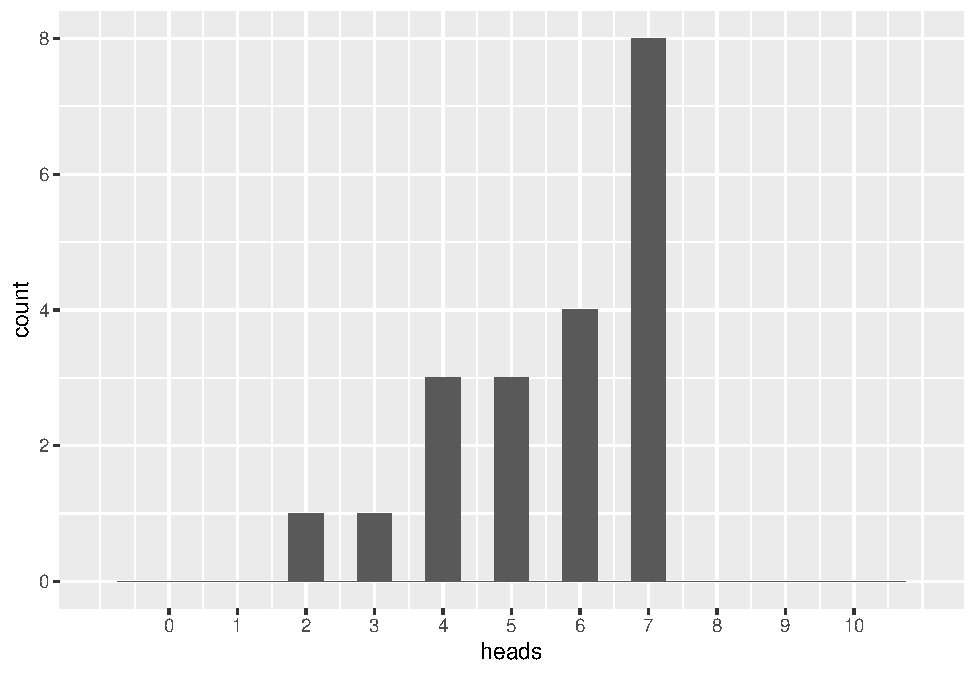
\includegraphics{intro_stats_files/figure-latex/unnamed-chunk-224-1.pdf}

And now the same histogram, but with proportions:

\begin{Shaded}
\begin{Highlighting}[]
\FunctionTok{ggplot}\NormalTok{(coin\_flips\_2000\_1000, }\FunctionTok{aes}\NormalTok{(}\AttributeTok{x =}\NormalTok{ prop)) }\SpecialCharTok{+}
    \FunctionTok{geom\_histogram}\NormalTok{(}\AttributeTok{binwidth =} \FloatTok{0.01}\NormalTok{, }\AttributeTok{boundary =} \FloatTok{0.5}\NormalTok{)}
\end{Highlighting}
\end{Shaded}

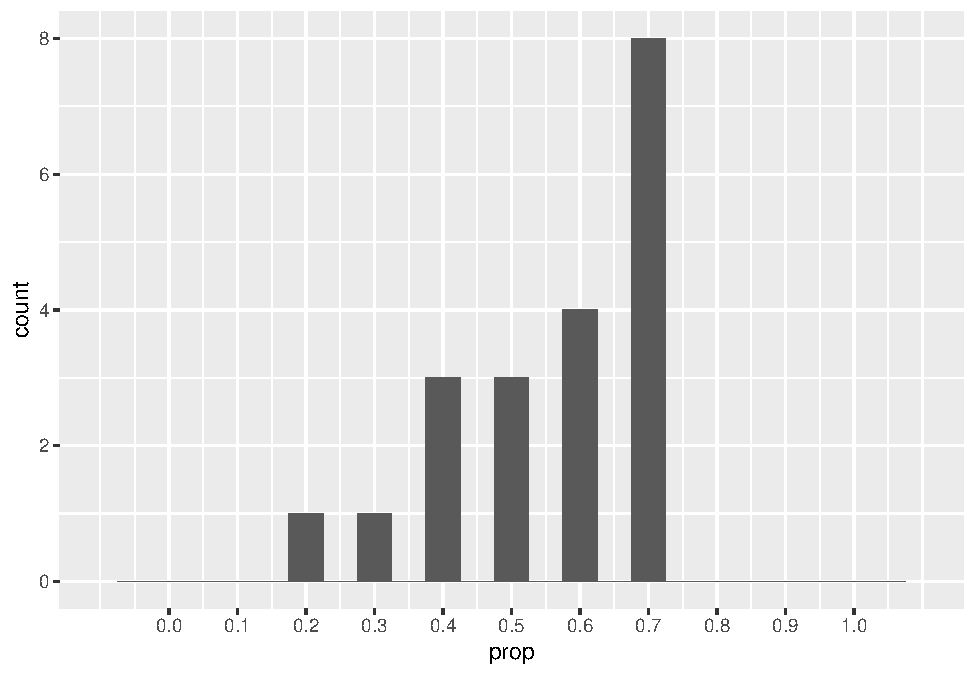
\includegraphics{intro_stats_files/figure-latex/unnamed-chunk-225-1.pdf}

\hypertarget{exercise-4-4}{%
\paragraph*{Exercise 4}\label{exercise-4-4}}
\addcontentsline{toc}{paragraph}{Exercise 4}

Comment on the histogram above. Describe its shape using the vocabulary of the three important features (modes, symmetry, outliers). Why do you think it's shaped like this?

Please write up your answer here.

\hypertarget{exercise-5-4}{%
\paragraph*{Exercise 5}\label{exercise-5-4}}
\addcontentsline{toc}{paragraph}{Exercise 5}

Given the amount of randomness involved (each person is tossing coins which randomly come up heads or tails), why do we see so much structure and orderliness in the histograms?

Please write up your answer here.

\hypertarget{randomization1-who-cares}{%
\section{But who cares about coin flips?}\label{randomization1-who-cares}}

It's fair to ask why we go to all this trouble to talk about coin flips. The most pressing research questions of our day do not involve people sitting around and flipping coins, either physically or virtually.

But now substitute ``heads'' and ``tails'' with ``cancer'' and ``no cancer''. Or ``guilty'' and ``not guilty''. Or ``shot'' and ``not shot''. The fact is that many important issues are measured as variables with two possible outcomes. There is some underlying ``probability'' of seeing one outcome over the other. (It doesn't have to be 50\% like the coin.) Statistical methods---including simulation---can say a lot about what we ``expect'' to see if these outcomes are truly random. More importantly, when we see outcomes that \emph{aren't} consistent with our simulations, we may wonder if there is some underlying mechanism that may be not so random after all. It may not look like it on first blush, but this idea is at the core of the scientific method.

For example, let's suppose that 85\% of U.S. adults support some form of background checks for gun buyers.\footnote{This is likely close to the truth. See this article: \url{https://iop.harvard.edu/get-involved/harvard-political-review/vast-majority-americans-support-universal-background-checks}} Now, imagine we went out and surveyed a random group of people and asked them a simple yes/no question about their support for background checks. What might we see?

Let's simulate. Imagine flipping a coin, but instead of coming up heads 50\% of the time, suppose it were possible for the coin to come up heads 85\% of the time.\footnote{The idea of a ``weighted'' coin that can do this comes up all the time in probability and statistics courses, but it seems that it's not likely one could actually manufacture a coin that came up heads more or less than 50\% of the time when flipped. See this paper for more details: \url{http://www.stat.columbia.edu/~gelman/research/published/diceRev2.pdf}} A sequence of heads and tails with this weird coin would be much like randomly surveying people and asking them about background checks.

We can make a ``virtual'' weird coin with the \texttt{rflip} command by specifying how often we want heads to come up.

\begin{Shaded}
\begin{Highlighting}[]
\FunctionTok{set.seed}\NormalTok{(}\DecValTok{1234}\NormalTok{)}
\FunctionTok{rflip}\NormalTok{(}\DecValTok{1}\NormalTok{, }\AttributeTok{prob =} \FloatTok{0.85}\NormalTok{)}
\end{Highlighting}
\end{Shaded}

\begin{verbatim}
## 
## Flipping 1 coin [ Prob(Heads) = 0.85 ] ...
## 
## H
## 
## Number of Heads: 1 [Proportion Heads: 1]
\end{verbatim}

If we flip our weird coin a bunch of times, we can see that our coin is not fair. Indeed, it appears to come up heads way more often than not:

\begin{Shaded}
\begin{Highlighting}[]
\FunctionTok{set.seed}\NormalTok{(}\DecValTok{1234}\NormalTok{)}
\FunctionTok{rflip}\NormalTok{(}\DecValTok{100}\NormalTok{, }\AttributeTok{prob =} \FloatTok{0.85}\NormalTok{)}
\end{Highlighting}
\end{Shaded}

\begin{verbatim}
## 
## Flipping 100 coins [ Prob(Heads) = 0.85 ] ...
## 
## H H H H T H H H H H H H H T H H H H H H H H H H H H H T H H H H H H H H
## H H T H H H H H H H H H H H H H H H H H H H H H T H H H H H H H H H H T
## H H H H H H H H T H H H H T H H H T H T H H H H H H H H
## 
## Number of Heads: 90 [Proportion Heads: 0.9]
\end{verbatim}

The results from the above code can be thought of as a survey of 100 random U.S. adults about their support for background checks for purchasing guns. ``Heads'' means ``supports'' and ``tails'' means ``opposes.'' If the majority of Americans support background checks, then we will come across more people in our survey who tell us they support background checks. This shows up in our simulation as the appearance of more heads than tails.

Note that there is no guarantee that our sample will have exactly 85\% heads. In fact, it doesn't; it has 90\% heads.

Again, keep in mind that we're simulating the act of obtaining a random sample of 100 U.S. adults. If we get a different sample, we'll get different results. (We set a different seed here. That ensures that this code chunk is randomly different from the one above.)

\begin{Shaded}
\begin{Highlighting}[]
\FunctionTok{set.seed}\NormalTok{(}\DecValTok{123456}\NormalTok{)}
\FunctionTok{rflip}\NormalTok{(}\DecValTok{100}\NormalTok{, }\AttributeTok{prob =} \FloatTok{0.85}\NormalTok{)}
\end{Highlighting}
\end{Shaded}

\begin{verbatim}
## 
## Flipping 100 coins [ Prob(Heads) = 0.85 ] ...
## 
## H H H H H H H H T H H H T T T T T H H H H H H H H H T T T H H T H H H H
## T T H H H H T H H H H H H H H H H T H T H H H H H H H H H H H H H H H H
## T H H H T H H H H H H T H H H H H H H H H H H H T H H H
## 
## Number of Heads: 81 [Proportion Heads: 0.81]
\end{verbatim}

See, this time, only 81\% came up heads, even though we expected 85\%. That's how randomness works.

\hypertarget{exercise-6a-2}{%
\paragraph*{Exercise 6(a)}\label{exercise-6a-2}}
\addcontentsline{toc}{paragraph}{Exercise 6(a)}

Now imagine that 2000 people all go out and conduct surveys of 100 random U.S. adults, asking them about their support for background checks. Write some R code that simulates this. Plot a histogram of the results. (Hint: you'll need \texttt{do(2000)\ *} in there.) Use the proportion of supporters (\texttt{prop}), not the raw count of supporters (\texttt{heads}).

\begin{Shaded}
\begin{Highlighting}[]
\FunctionTok{set.seed}\NormalTok{(}\DecValTok{1234}\NormalTok{)}
\CommentTok{\# Add code here to simulate 2000 surveys of 100 U.S. adults.}
\end{Highlighting}
\end{Shaded}

\begin{Shaded}
\begin{Highlighting}[]
\CommentTok{\# Plot the results in a histogram using proportions.}
\end{Highlighting}
\end{Shaded}

\hypertarget{exercise-6b-2}{%
\paragraph*{Exercise 6(b)}\label{exercise-6b-2}}
\addcontentsline{toc}{paragraph}{Exercise 6(b)}

Run another simulation, but this time, have each person survey 1000 adults and not just 100.

\begin{Shaded}
\begin{Highlighting}[]
\FunctionTok{set.seed}\NormalTok{(}\DecValTok{1234}\NormalTok{)}
\CommentTok{\# Add code here to simulate 2000 surveys of 1000 U.S. adults.}
\end{Highlighting}
\end{Shaded}

\begin{Shaded}
\begin{Highlighting}[]
\CommentTok{\# Plot the results in a histogram using proportions.}
\end{Highlighting}
\end{Shaded}

\hypertarget{exercise-6c}{%
\paragraph*{Exercise 6(c)}\label{exercise-6c}}
\addcontentsline{toc}{paragraph}{Exercise 6(c)}

What changed when you surveyed 1000 people instead of 100?

Please write up your answer here.

\hypertarget{randomization1-sampling-var}{%
\section{Sampling variability}\label{randomization1-sampling-var}}

We've seen that taking repeated samples (using the \texttt{do} command) leads to lots of different outcomes. That is randomness in action. We don't expect the results of each survey to be exactly the same every time the survey is administered.

But despite this randomness, there is an interesting pattern that we can observe. It has to do with the number of times we flip the coin. Since we're using coin flips to simulate the act of conducting a survey, the number of coin flips is playing the role of the \emph{sample size}. In other words, if we want to simulate a survey of U.S. adults with a sample size of 100, we simulate that by flipping 100 coins.

\hypertarget{exercise-7-2}{%
\paragraph*{Exercise 7}\label{exercise-7-2}}
\addcontentsline{toc}{paragraph}{Exercise 7}

Go back and look at all the examples above. What do you notice about the range of values on the x-axis when the sample size is small versus large? (In other words, in what way are the histograms different when using \texttt{rflip(10)} or \texttt{rflip(100)} versus \texttt{rflip(1000)}? It's easier to compare histograms one to another when looking at the proportions instead of the raw head counts because proportions are always on the same scale from 0 to 1.)

Please write up your answer here.

\hypertarget{randomization1-conclusion}{%
\section{Conclusion}\label{randomization1-conclusion}}

Simulation is a tool for understanding what happens when a statistical process is repeated many times in a randomized way. The availability of fast computer processing makes simulation easy and accessible. Eventually, the goal will be to use simulation to answer important questions about data and the processes in the world that generate data. This is possible because, despite the ubiquitous presence of randomness, a certain order emerges when the number of samples is large enough. Even though there is sampling variability (different random outcomes each time we sample), there are patterns in that variability that can be exploited to make predictions.

\hypertarget{randomization2}{%
\chapter{Introduction to randomization, Part 2}\label{randomization2}}

2.0

\hypertarget{functions-introduced-in-this-chapter-8}{%
\subsection*{Functions introduced in this chapter}\label{functions-introduced-in-this-chapter-8}}
\addcontentsline{toc}{subsection}{Functions introduced in this chapter}

\texttt{sample}, \texttt{specify}, \texttt{hypothesize}, \texttt{generate}, \texttt{calculate}, \texttt{visualize}, \texttt{shade\_p\_value}, \texttt{get\_p\_value}

\hypertarget{randomization2-intro}{%
\section{Introduction}\label{randomization2-intro}}

In this chapter, we'll learn more about randomization and simulation. Instead of flipping coins, though, we'll randomly shuffle data around in order to explore the effects of randomizing a predictor variable.

\hypertarget{randomization2-install}{%
\subsection{Install new packages}\label{randomization2-install}}

If you are using RStudio Workbench, you do not need to install any packages. (Any packages you need should already be installed by the server administrators.)

If you are using R and RStudio on your own machine instead of accessing RStudio Workbench through a browser, you'll need to type the following commands at the Console:

\begin{verbatim}
install.packages("openintro")
install.packages("infer")
\end{verbatim}

\hypertarget{randomization2-download}{%
\subsection{Download the R notebook file}\label{randomization2-download}}

Check the upper-right corner in RStudio to make sure you're in your \texttt{intro\_stats} project. Then click on the following link to download this chapter as an R notebook file (\texttt{.Rmd}).

https://vectorposse.github.io/intro\_stats/chapter\_downloads/09-intro\_to\_randomization\_2.Rmd

Once the file is downloaded, move it to your project folder in RStudio and open it there.

\hypertarget{randomization2-restart}{%
\subsection{Restart R and run all chunks}\label{randomization2-restart}}

In RStudio, select ``Restart R and Run All Chunks'' from the ``Run'' menu.

\hypertarget{randomization2-load}{%
\section{Load packages}\label{randomization2-load}}

We'll load \texttt{tidyverse} as usual along with the \texttt{janitor} package to make tables (with \texttt{tabyl}). The \texttt{openintro} package has a data set called \texttt{sex\_discrimination} that we will explore. Finally, the \texttt{infer} package will provide tools that we will use in nearly every chapter for the remainder of the book.

\begin{Shaded}
\begin{Highlighting}[]
\FunctionTok{library}\NormalTok{(tidyverse)}
\FunctionTok{library}\NormalTok{(janitor)}
\FunctionTok{library}\NormalTok{(openintro)}
\end{Highlighting}
\end{Shaded}

\begin{verbatim}
## Loading required package: airports
\end{verbatim}

\begin{verbatim}
## Loading required package: cherryblossom
\end{verbatim}

\begin{verbatim}
## Loading required package: usdata
\end{verbatim}

\begin{verbatim}
## 
## Attaching package: 'openintro'
\end{verbatim}

\begin{verbatim}
## The following object is masked from 'package:mosaic':
## 
##     dotPlot
\end{verbatim}

\begin{verbatim}
## The following objects are masked from 'package:lattice':
## 
##     ethanol, lsegments
\end{verbatim}

\begin{verbatim}
## The following object is masked from 'package:faraway':
## 
##     orings
\end{verbatim}

\begin{Shaded}
\begin{Highlighting}[]
\FunctionTok{library}\NormalTok{(infer)}
\end{Highlighting}
\end{Shaded}

\begin{verbatim}
## 
## Attaching package: 'infer'
\end{verbatim}

\begin{verbatim}
## The following objects are masked from 'package:mosaic':
## 
##     prop_test, t_test
\end{verbatim}

\hypertarget{randomization2-question}{%
\section{Our research question}\label{randomization2-question}}

An interesting study was conducted in the 1970s that investigated gender discrimination in hiring.\footnote{Rosen B and Jerdee T. 1974. Influence of sex role stereotypes on personnel decisions. \emph{Journal of Applied Psychology} 59(1):9-14.} The researchers brought in 48 male bank supervisors and asked them to evaluate personnel files. Based on their review, they were to determine if the person was qualified for promotion to branch manager. The trick is that all the files were identical, but half listed the candidate as male and half listed the candidate as female. The files were randomly assigned to the 48 supervisors.

The research question is whether the files supposedly belonging to males were recommended for promotion more than the files supposedly belonging to females.

\hypertarget{exercise-1-6}{%
\paragraph*{Exercise 1}\label{exercise-1-6}}
\addcontentsline{toc}{paragraph}{Exercise 1}

Is the study described above an observational study or an experiment? How do you know?

Please write up your answer here.

\hypertarget{exercise-2a-1}{%
\paragraph*{Exercise 2(a)}\label{exercise-2a-1}}
\addcontentsline{toc}{paragraph}{Exercise 2(a)}

Identify the sample in the study. In other words, how many people were in the sample and what are the important characteristics common to those people.

Please write up your answer here.

\hypertarget{exercise-2b-1}{%
\paragraph*{Exercise 2(b)}\label{exercise-2b-1}}
\addcontentsline{toc}{paragraph}{Exercise 2(b)}

Identify the population of interest in the study. In other words, who is the sample supposed to represent? That is, what group of people that this study is trying to learn about?

Please write up your answer here.

\hypertarget{exercise-2c-1}{%
\paragraph*{Exercise 2(c)}\label{exercise-2c-1}}
\addcontentsline{toc}{paragraph}{Exercise 2(c)}

In your opinion, does the sample from this study truly represent the population you identified above?

Please write up your answer here.

\hypertarget{randomization2-eda}{%
\section{Exploratory data analysis}\label{randomization2-eda}}

Here is the data:

\begin{Shaded}
\begin{Highlighting}[]
\NormalTok{sex\_discrimination}
\end{Highlighting}
\end{Shaded}

\begin{verbatim}
## # A tibble: 48 x 2
##    sex   decision
##    <fct> <fct>   
##  1 male  promoted
##  2 male  promoted
##  3 male  promoted
##  4 male  promoted
##  5 male  promoted
##  6 male  promoted
##  7 male  promoted
##  8 male  promoted
##  9 male  promoted
## 10 male  promoted
## # ... with 38 more rows
\end{verbatim}

\begin{Shaded}
\begin{Highlighting}[]
\FunctionTok{glimpse}\NormalTok{(sex\_discrimination)}
\end{Highlighting}
\end{Shaded}

\begin{verbatim}
## Rows: 48
## Columns: 2
## $ sex      <fct> male, male, male, male, male, male, male, male, male, male, m~
## $ decision <fct> promoted, promoted, promoted, promoted, promoted, promoted, p~
\end{verbatim}

\hypertarget{exercise-3-5}{%
\paragraph*{Exercise 3}\label{exercise-3-5}}
\addcontentsline{toc}{paragraph}{Exercise 3}

Which variable is the response variable and which variable is the predictor variable?

Please write up your answer here.

\begin{center}\rule{0.5\linewidth}{0.5pt}\end{center}

Here is a contingency table with \texttt{decision} as the row variable and \texttt{sex} as the column variable. (Recall that we always list the response variable first. That way, the column sums will show us how many are in each of the predictor groups.)

\begin{Shaded}
\begin{Highlighting}[]
\FunctionTok{tabyl}\NormalTok{(sex\_discrimination, decision, sex) }\SpecialCharTok{\%\textgreater{}\%}
    \FunctionTok{adorn\_totals}\NormalTok{()}
\end{Highlighting}
\end{Shaded}

\begin{verbatim}
##      decision male female
##      promoted   21     14
##  not promoted    3     10
##         Total   24     24
\end{verbatim}

\hypertarget{exercise-4-5}{%
\paragraph*{Exercise 4}\label{exercise-4-5}}
\addcontentsline{toc}{paragraph}{Exercise 4}

Create another contingency table of \texttt{decision} and \texttt{sex}, this time with percentages (\emph{not} proportions) instead of counts. You'll probably have to go back to the ``Categorical data'' to review the syntax. (Hint: you should have three separate \texttt{adorn} functions on the lines following the \texttt{tabyl} command.)

\begin{Shaded}
\begin{Highlighting}[]
\CommentTok{\# Add code here to create a contingency table of percentages}
\end{Highlighting}
\end{Shaded}

\begin{center}\rule{0.5\linewidth}{0.5pt}\end{center}

Although we can read off the percentages in the contingency table, we need to do computations using the proportions. (Remember that we use percentages to communicate with other human beings, but we do math with proportions.) Fortunately, the output of \texttt{tabyl} is a tibble! So we can manipulate and grab the elements we need.

Let's create and store the \texttt{tabyl} output with proportions. We don't need the marginal distribution, so we can dispense with \texttt{adorn\_totals}.

\begin{Shaded}
\begin{Highlighting}[]
\NormalTok{decision\_sex\_tabyl }\OtherTok{\textless{}{-}} \FunctionTok{tabyl}\NormalTok{(sex\_discrimination, decision, sex) }\SpecialCharTok{\%\textgreater{}\%}
    \FunctionTok{adorn\_percentages}\NormalTok{(}\StringTok{"col"}\NormalTok{)}
\NormalTok{decision\_sex\_tabyl}
\end{Highlighting}
\end{Shaded}

\begin{verbatim}
##      decision  male    female
##      promoted 0.875 0.5833333
##  not promoted 0.125 0.4166667
\end{verbatim}

\hypertarget{exercise-5-5}{%
\paragraph*{Exercise 5}\label{exercise-5-5}}
\addcontentsline{toc}{paragraph}{Exercise 5}

Interpret these proportions in the context of the data. In other words, what do these proportions say about the male files that were recommended for promotion versus the female files recommended for promotion?

Please write up your answer here.

\begin{center}\rule{0.5\linewidth}{0.5pt}\end{center}

The real statistic of interest to us is the difference between these proportions. We can use the \texttt{mutate} command from \texttt{dplyr} variable compute the difference for us.

\begin{Shaded}
\begin{Highlighting}[]
\NormalTok{decision\_sex\_tabyl }\SpecialCharTok{\%\textgreater{}\%}
    \FunctionTok{mutate}\NormalTok{(}\AttributeTok{diff =}\NormalTok{ male }\SpecialCharTok{{-}}\NormalTok{ female)}
\end{Highlighting}
\end{Shaded}

\begin{verbatim}
##      decision  male    female       diff
##      promoted 0.875 0.5833333  0.2916667
##  not promoted 0.125 0.4166667 -0.2916667
\end{verbatim}

As a matter of fact, once we know the difference in promotion rates, we don't really need the individual proportions anymore. The \texttt{transmute} verb is a version of \texttt{mutate} that gives us exactly what we want. It will create a new column just like \texttt{mutate}, but then it keeps only that new column. We'll call the resulting output \texttt{decision\_sex\_diff}.

\begin{Shaded}
\begin{Highlighting}[]
\NormalTok{decision\_sex\_diff }\OtherTok{\textless{}{-}}\NormalTok{ decision\_sex\_tabyl }\SpecialCharTok{\%\textgreater{}\%}
    \FunctionTok{transmute}\NormalTok{(}\AttributeTok{diff =}\NormalTok{ male }\SpecialCharTok{{-}}\NormalTok{ female)}
\NormalTok{decision\_sex\_diff}
\end{Highlighting}
\end{Shaded}

\begin{verbatim}
##        diff
##   0.2916667
##  -0.2916667
\end{verbatim}

We don't really need both the positive and negative values. Let's just keep the first row and keep track of which direction we subtracted to get it. (The positive difference results from the male promotion rate minus the female promotion rate.) We can use \texttt{slice} to grab the first row:

\begin{Shaded}
\begin{Highlighting}[]
\NormalTok{decision\_sex\_diff }\SpecialCharTok{\%\textgreater{}\%}
    \FunctionTok{slice}\NormalTok{(}\DecValTok{1}\NormalTok{)}
\end{Highlighting}
\end{Shaded}

\begin{verbatim}
##       diff
##  0.2916667
\end{verbatim}

This means that there is a 29\% difference between the male files that were promoted and the female files that were promoted. The difference was computed as males minus females, so the fact that the number is positive means that male files were \emph{more} likely to recommended for promotion.

\hypertarget{randomization2-permuting}{%
\section{Permuting}\label{randomization2-permuting}}

One way to see if there is evidence of an association between promotion decisions and sex is to assume, temporarily, that there is no association. If there were truly no association, then the difference between the promotion rates between the male files and female files should be 0\%. Of course, the number of people promoted in the data was 35, an odd number, so the number of male files promoted and female files promoted cannot be the same. Therefore, the difference in proportions can't be exactly 0 in this data. Nevertheless, we would expect---under the assumption of no association---the number of male files promoted to be \emph{close} to the number of female files promoted, giving a difference around 0\%.

Now, we saw a difference of about 29\% between the two groups in the data. Then again, non-zero differences---sometimes even large ones--- can just come about by pure chance alone. We may have accidentally sampled more bank managers who just happened to prefer the male candidates. This could happen for sexist reasons; it's possible our sample of bank managers are, by chance, more sexist than bank managers in the general population during the 1970s. Or it might be for more benign reasons; perhaps the male applications got randomly steered to bank managers who were more likely to be impressed with any application, and therefore, they were more likely to promote anyone regardless of the gender listed. We have to consider the possibility that our observed difference seems large even though there may have been no association between promotion and sex in the general population.

So how do we test the range of values that could arise from just chance alone? In other words, how do we explore sampling variability?

One way to force the variables to be independent is to ``permute''---in other words, shuffle---the values of \texttt{sex} in our data. If we ignore the sex listed in the file and give it a random label (independent of the \emph{actual} sex listed in the file), we know for sure that such an assignment is random and not due to any actual evidence of sexism. In that case, promotion is equally likely to occur in both groups.

Let's see how permuting works in R. To begin with, look at the actual values of \texttt{sex} in our data:

\begin{Shaded}
\begin{Highlighting}[]
\NormalTok{sex\_discrimination}\SpecialCharTok{$}\NormalTok{sex}
\end{Highlighting}
\end{Shaded}

\begin{verbatim}
##  [1] male   male   male   male   male   male   male   male   male   male  
## [11] male   male   male   male   male   male   male   male   male   male  
## [21] male   male   male   male   female female female female female female
## [31] female female female female female female female female female female
## [41] female female female female female female female female
## Levels: male female
\end{verbatim}

All the males happen to be listed first, followed by all the females.

Now we permute all the values around (using the \texttt{sample} command). As explained in an earlier chapter, we will set the seed so that our results are reproducible.

\begin{Shaded}
\begin{Highlighting}[]
\FunctionTok{set.seed}\NormalTok{(}\DecValTok{3141593}\NormalTok{)}
\FunctionTok{sample}\NormalTok{(sex\_discrimination}\SpecialCharTok{$}\NormalTok{sex)}
\end{Highlighting}
\end{Shaded}

\begin{verbatim}
##  [1] male   female male   male   female female female female female female
## [11] female female female female male   male   female male   female male  
## [21] female female male   male   female female male   female male   male  
## [31] male   male   male   female male   female male   male   male   male  
## [41] female female female male   male   male   female male  
## Levels: male female
\end{verbatim}

Do it again without the seed, just to make sure it's truly random:

\begin{Shaded}
\begin{Highlighting}[]
\FunctionTok{sample}\NormalTok{(sex\_discrimination}\SpecialCharTok{$}\NormalTok{sex)}
\end{Highlighting}
\end{Shaded}

\begin{verbatim}
##  [1] male   male   male   female male   female male   female female female
## [11] female male   female male   female female female female male   male  
## [21] female female female male   male   female male   male   male   female
## [31] male   male   male   male   male   female female female female male  
## [41] female female male   male   male   female female male  
## Levels: male female
\end{verbatim}

\hypertarget{randomization2-randomization}{%
\section{Randomization}\label{randomization2-randomization}}

The idea here is to keep the promotion status the same for each file, but randomly permute the sex labels. There will still be the same number of male and female files, but now they will be randomly matched with promoted files and not promoted files. Since this new grouping into ``males'' and ``females'' is completely random and arbitrary, we expect the likelihood of promotion to be equal for both groups.

A more precise way of saying this is that the expected difference under the assumption of independent variables is 0\%. If there were truly no association, then the percentage of people promoted would be independent of sex. However, sampling variability means that we are not likely to see an exact difference of 0\%. (Also, as we mentioned earlier, the odd number of promotions means the difference will never be exactly 0\% anyway in this data.) The real question, then, is how different could the difference be from 0\% and still be reasonably possible due to random chance.

Let's perform a few random simulations. We'll walk through the steps one line at a time. The first thing we do is permute the \texttt{sex} column:

\begin{Shaded}
\begin{Highlighting}[]
\FunctionTok{set.seed}\NormalTok{(}\DecValTok{3141593}\NormalTok{)}
\NormalTok{sex\_discrimination }\SpecialCharTok{\%\textgreater{}\%}
    \FunctionTok{mutate}\NormalTok{(}\AttributeTok{sex =} \FunctionTok{sample}\NormalTok{(sex))}
\end{Highlighting}
\end{Shaded}

\begin{verbatim}
## # A tibble: 48 x 2
##    sex    decision
##    <fct>  <fct>   
##  1 male   promoted
##  2 female promoted
##  3 male   promoted
##  4 male   promoted
##  5 female promoted
##  6 female promoted
##  7 female promoted
##  8 female promoted
##  9 female promoted
## 10 female promoted
## # ... with 38 more rows
\end{verbatim}

Then we follow the steps from earlier, generating a contingency table with proportions. This is accomplished by simply adding two lines of code to the previous code:

\begin{Shaded}
\begin{Highlighting}[]
\FunctionTok{set.seed}\NormalTok{(}\DecValTok{3141593}\NormalTok{)}
\NormalTok{sex\_discrimination }\SpecialCharTok{\%\textgreater{}\%}
    \FunctionTok{mutate}\NormalTok{(}\AttributeTok{sex =} \FunctionTok{sample}\NormalTok{(sex)) }\SpecialCharTok{\%\textgreater{}\%}
    \FunctionTok{tabyl}\NormalTok{(decision, sex) }\SpecialCharTok{\%\textgreater{}\%}
    \FunctionTok{adorn\_percentages}\NormalTok{(}\StringTok{"col"}\NormalTok{)}
\end{Highlighting}
\end{Shaded}

\begin{verbatim}
##      decision      male    female
##      promoted 0.6666667 0.7916667
##  not promoted 0.3333333 0.2083333
\end{verbatim}

Note that the proportions in this table are different from the ones in the real data.

Then we calculate the difference between the male and female columns by adding a line with \texttt{transmute}:

\begin{Shaded}
\begin{Highlighting}[]
\FunctionTok{set.seed}\NormalTok{(}\DecValTok{3141593}\NormalTok{)}
\NormalTok{sex\_discrimination }\SpecialCharTok{\%\textgreater{}\%}
    \FunctionTok{mutate}\NormalTok{(}\AttributeTok{sex =} \FunctionTok{sample}\NormalTok{(sex)) }\SpecialCharTok{\%\textgreater{}\%}
    \FunctionTok{tabyl}\NormalTok{(decision, sex) }\SpecialCharTok{\%\textgreater{}\%}
    \FunctionTok{adorn\_percentages}\NormalTok{(}\StringTok{"col"}\NormalTok{) }\SpecialCharTok{\%\textgreater{}\%}
    \FunctionTok{transmute}\NormalTok{(}\AttributeTok{diff =}\NormalTok{ male }\SpecialCharTok{{-}}\NormalTok{ female)}
\end{Highlighting}
\end{Shaded}

\begin{verbatim}
##    diff
##  -0.125
##   0.125
\end{verbatim}

In this case, the first row happens to be negative, but that's okay. This particular random shuffling had more females promoted than males. (Remember, though, that the permuted sex labels are now meaningless.)

Finally, we grab the entry in the first row with \texttt{slice}:

\begin{Shaded}
\begin{Highlighting}[]
\FunctionTok{set.seed}\NormalTok{(}\DecValTok{3141593}\NormalTok{)}
\NormalTok{sex\_discrimination }\SpecialCharTok{\%\textgreater{}\%}
    \FunctionTok{mutate}\NormalTok{(}\AttributeTok{sex =} \FunctionTok{sample}\NormalTok{(sex)) }\SpecialCharTok{\%\textgreater{}\%}
    \FunctionTok{tabyl}\NormalTok{(decision, sex) }\SpecialCharTok{\%\textgreater{}\%}
    \FunctionTok{adorn\_percentages}\NormalTok{(}\StringTok{"col"}\NormalTok{) }\SpecialCharTok{\%\textgreater{}\%}
    \FunctionTok{transmute}\NormalTok{(}\AttributeTok{diff =}\NormalTok{ male }\SpecialCharTok{{-}}\NormalTok{ female) }\SpecialCharTok{\%\textgreater{}\%}
    \FunctionTok{slice}\NormalTok{(}\DecValTok{1}\NormalTok{)}
\end{Highlighting}
\end{Shaded}

\begin{verbatim}
##    diff
##  -0.125
\end{verbatim}

We'll repeat this code a few more times, but without the seed, to get new random observations.

\begin{Shaded}
\begin{Highlighting}[]
\NormalTok{sex\_discrimination }\SpecialCharTok{\%\textgreater{}\%}
    \FunctionTok{mutate}\NormalTok{(}\AttributeTok{sex =} \FunctionTok{sample}\NormalTok{(sex)) }\SpecialCharTok{\%\textgreater{}\%}
    \FunctionTok{tabyl}\NormalTok{(decision, sex) }\SpecialCharTok{\%\textgreater{}\%}
    \FunctionTok{adorn\_percentages}\NormalTok{(}\StringTok{"col"}\NormalTok{) }\SpecialCharTok{\%\textgreater{}\%}
    \FunctionTok{transmute}\NormalTok{(}\AttributeTok{diff =}\NormalTok{ male }\SpecialCharTok{{-}}\NormalTok{ female) }\SpecialCharTok{\%\textgreater{}\%}
    \FunctionTok{slice}\NormalTok{(}\DecValTok{1}\NormalTok{)}
\end{Highlighting}
\end{Shaded}

\begin{verbatim}
##        diff
##  0.04166667
\end{verbatim}

\begin{Shaded}
\begin{Highlighting}[]
\NormalTok{sex\_discrimination }\SpecialCharTok{\%\textgreater{}\%}
    \FunctionTok{mutate}\NormalTok{(}\AttributeTok{sex =} \FunctionTok{sample}\NormalTok{(sex)) }\SpecialCharTok{\%\textgreater{}\%}
    \FunctionTok{tabyl}\NormalTok{(decision, sex) }\SpecialCharTok{\%\textgreater{}\%}
    \FunctionTok{adorn\_percentages}\NormalTok{(}\StringTok{"col"}\NormalTok{) }\SpecialCharTok{\%\textgreater{}\%}
    \FunctionTok{transmute}\NormalTok{(}\AttributeTok{diff =}\NormalTok{ male }\SpecialCharTok{{-}}\NormalTok{ female) }\SpecialCharTok{\%\textgreater{}\%}
    \FunctionTok{slice}\NormalTok{(}\DecValTok{1}\NormalTok{)}
\end{Highlighting}
\end{Shaded}

\begin{verbatim}
##   diff
##  0.125
\end{verbatim}

\begin{Shaded}
\begin{Highlighting}[]
\NormalTok{sex\_discrimination }\SpecialCharTok{\%\textgreater{}\%}
    \FunctionTok{mutate}\NormalTok{(}\AttributeTok{sex =} \FunctionTok{sample}\NormalTok{(sex)) }\SpecialCharTok{\%\textgreater{}\%}
    \FunctionTok{tabyl}\NormalTok{(decision, sex) }\SpecialCharTok{\%\textgreater{}\%}
    \FunctionTok{adorn\_percentages}\NormalTok{(}\StringTok{"col"}\NormalTok{) }\SpecialCharTok{\%\textgreater{}\%}
    \FunctionTok{transmute}\NormalTok{(}\AttributeTok{diff =}\NormalTok{ male }\SpecialCharTok{{-}}\NormalTok{ female) }\SpecialCharTok{\%\textgreater{}\%}
    \FunctionTok{slice}\NormalTok{(}\DecValTok{1}\NormalTok{)}
\end{Highlighting}
\end{Shaded}

\begin{verbatim}
##   diff
##  0.125
\end{verbatim}

\begin{Shaded}
\begin{Highlighting}[]
\NormalTok{sex\_discrimination }\SpecialCharTok{\%\textgreater{}\%}
    \FunctionTok{mutate}\NormalTok{(}\AttributeTok{sex =} \FunctionTok{sample}\NormalTok{(sex)) }\SpecialCharTok{\%\textgreater{}\%}
    \FunctionTok{tabyl}\NormalTok{(decision, sex) }\SpecialCharTok{\%\textgreater{}\%}
    \FunctionTok{adorn\_percentages}\NormalTok{(}\StringTok{"col"}\NormalTok{) }\SpecialCharTok{\%\textgreater{}\%}
    \FunctionTok{transmute}\NormalTok{(}\AttributeTok{diff =}\NormalTok{ male }\SpecialCharTok{{-}}\NormalTok{ female) }\SpecialCharTok{\%\textgreater{}\%}
    \FunctionTok{slice}\NormalTok{(}\DecValTok{1}\NormalTok{)}
\end{Highlighting}
\end{Shaded}

\begin{verbatim}
##        diff
##  -0.2916667
\end{verbatim}

Think carefully about what these random numbers mean. Each time we randomize, we get a simulated difference in the proportion of promotions between male files and female files. The \texttt{sample} part ensures that there is no actual relationship between promotion and sex among these randomized values. We expect each simulated difference to be close to zero, but we also expect deviations from zero due to randomness and chance.

\hypertarget{randomization2-infer}{%
\section{\texorpdfstring{The \texttt{infer} package}{The infer package}}\label{randomization2-infer}}

The above code examples show the nuts and bolts of permuting data around to break any association that might exist between two variables. However, to do a proper randomization, we need to repeat this process many, many times (just like how we flipped thousands of ``coins'' in the last chapter).

Here we introduce some code from the \texttt{infer} package that will help us automate this procedure. The added benefit of introducing \texttt{infer} now is that we will continue to use it in nearly every chapter of the book that follows.

Here is the code template, starting with setting the seed:

\begin{Shaded}
\begin{Highlighting}[]
\FunctionTok{set.seed}\NormalTok{(}\DecValTok{3141593}\NormalTok{)}
\NormalTok{sims }\OtherTok{\textless{}{-}}\NormalTok{ sex\_discrimination }\SpecialCharTok{\%\textgreater{}\%}
    \FunctionTok{specify}\NormalTok{(decision }\SpecialCharTok{\textasciitilde{}}\NormalTok{ sex, }\AttributeTok{success =} \StringTok{"promoted"}\NormalTok{) }\SpecialCharTok{\%\textgreater{}\%}
    \FunctionTok{hypothesize}\NormalTok{(}\AttributeTok{null =} \StringTok{"independence"}\NormalTok{) }\SpecialCharTok{\%\textgreater{}\%}
    \FunctionTok{generate}\NormalTok{(}\AttributeTok{reps =} \DecValTok{1000}\NormalTok{, }\AttributeTok{type =} \StringTok{"permute"}\NormalTok{) }\SpecialCharTok{\%\textgreater{}\%}
    \FunctionTok{calculate}\NormalTok{(}\AttributeTok{stat =} \StringTok{"diff in props"}\NormalTok{, }\AttributeTok{order =} \FunctionTok{c}\NormalTok{(}\StringTok{"male"}\NormalTok{, }\StringTok{"female"}\NormalTok{))}
\NormalTok{sims}
\end{Highlighting}
\end{Shaded}

\begin{verbatim}
## Response: decision (factor)
## Explanatory: sex (factor)
## Null Hypothesis: independence
## # A tibble: 1,000 x 2
##    replicate    stat
##        <int>   <dbl>
##  1         1 -0.125 
##  2         2 -0.125 
##  3         3 -0.0417
##  4         4  0.0417
##  5         5  0.125 
##  6         6 -0.0417
##  7         7 -0.0417
##  8         8  0.125 
##  9         9  0.125 
## 10        10  0.208 
## # ... with 990 more rows
\end{verbatim}

We will learn more about all these lines of code in future chapters. By the end of the course, running this type of analysis will be second nature. For now, you can copy and paste the code chunk above and make minor changes as you need. Here are the three things you will need to look out for for doing this with different data sets in the future:

\begin{enumerate}
\def\labelenumi{\arabic{enumi}.}
\tightlist
\item
  The second line (after setting the seed) will be your new data set.
\item
  In the \texttt{specify} line, you will have a different response variable, predictor variable, and success condition that will depend on the context of your new data.
\item
  In the \texttt{calculate} line, you will have two different levels that you want to compare. Be careful to list them in the order in which you want to subtract them.
\end{enumerate}

\hypertarget{randomization2-plot}{%
\section{Plot results}\label{randomization2-plot}}

A histogram will show us the range of possible values under the assumption of independence of the two variables. We can get one from our \texttt{infer} output using \texttt{visualize}. (This is a lot easier than building a histogram with \texttt{ggplot}!)

\begin{Shaded}
\begin{Highlighting}[]
\NormalTok{sims }\SpecialCharTok{\%\textgreater{}\%}
    \FunctionTok{visualize}\NormalTok{()}
\end{Highlighting}
\end{Shaded}

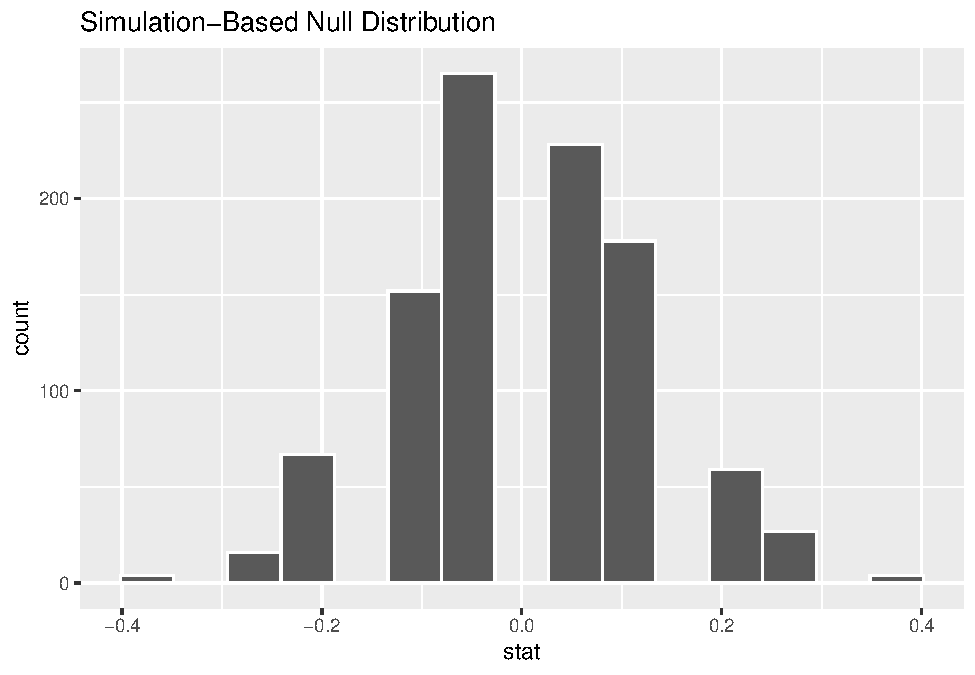
\includegraphics{intro_stats_files/figure-latex/unnamed-chunk-254-1.pdf}

The bins aren't great in the picture above. There is no way currently to set the binwidth or boundary as we've done before, but we can experiment with the total number of bins. 9 seems to be a good number.

\begin{Shaded}
\begin{Highlighting}[]
\NormalTok{sims }\SpecialCharTok{\%\textgreater{}\%}
    \FunctionTok{visualize}\NormalTok{(}\AttributeTok{bins =} \DecValTok{9}\NormalTok{)}
\end{Highlighting}
\end{Shaded}

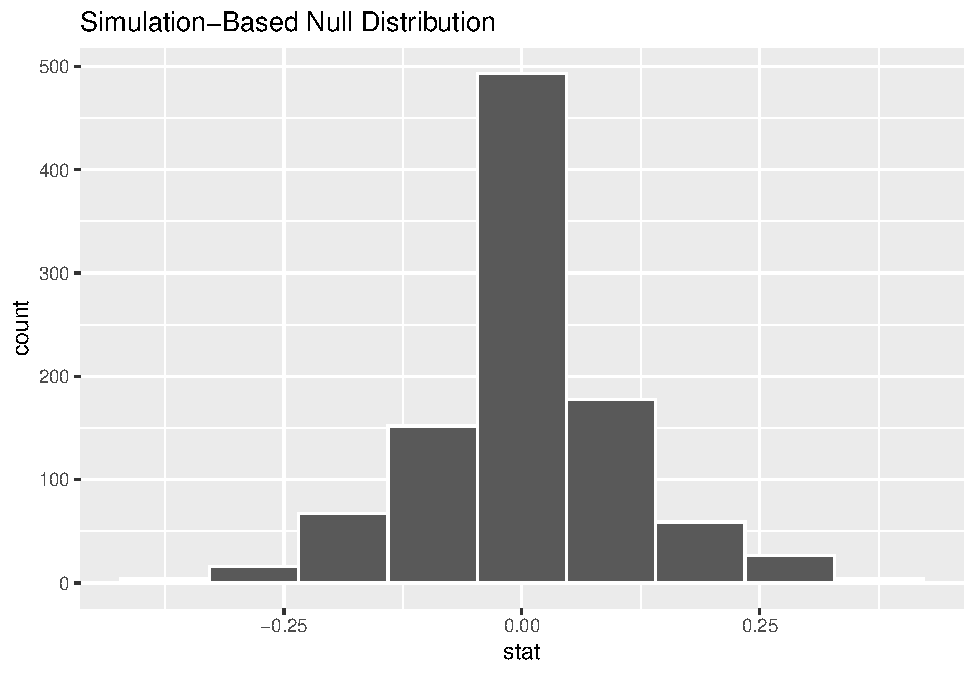
\includegraphics{intro_stats_files/figure-latex/unnamed-chunk-255-1.pdf}

\hypertarget{exercise-6-3}{%
\paragraph*{Exercise 6}\label{exercise-6-3}}
\addcontentsline{toc}{paragraph}{Exercise 6}

Why is the mode of the graph above at 0? This has been explained several different times in this chapter, but put it into your own words to make sure you understand the logic behind the randomization.

Please write up your answer here.

\begin{center}\rule{0.5\linewidth}{0.5pt}\end{center}

Let's compare these simulated values to the observed difference in the real data. We've computed the latter already, but let's use \texttt{infer} tools to find it. We'll give the answer a name, \texttt{obs\_diff}.

\begin{Shaded}
\begin{Highlighting}[]
\NormalTok{obs\_diff }\OtherTok{\textless{}{-}}\NormalTok{ sex\_discrimination }\SpecialCharTok{\%\textgreater{}\%}
    \FunctionTok{observe}\NormalTok{(decision }\SpecialCharTok{\textasciitilde{}}\NormalTok{ sex, }\AttributeTok{success =} \StringTok{"promoted"}\NormalTok{,}
            \AttributeTok{stat =} \StringTok{"diff in props"}\NormalTok{, }\AttributeTok{order =} \FunctionTok{c}\NormalTok{(}\StringTok{"male"}\NormalTok{, }\StringTok{"female"}\NormalTok{))}
\NormalTok{obs\_diff}
\end{Highlighting}
\end{Shaded}

\begin{verbatim}
## Response: decision (factor)
## Explanatory: sex (factor)
## # A tibble: 1 x 1
##    stat
##   <dbl>
## 1 0.292
\end{verbatim}

Now we can graph the observed difference in the data alongside the simulated values under the assumption of independent variables. The name of the function \texttt{shade\_p\_value} is a little cryptic for now, but it will become clear within a few chapters.

\begin{Shaded}
\begin{Highlighting}[]
\NormalTok{sims }\SpecialCharTok{\%\textgreater{}\%}
    \FunctionTok{visualize}\NormalTok{(}\AttributeTok{bins =} \DecValTok{9}\NormalTok{) }\SpecialCharTok{+}
    \FunctionTok{shade\_p\_value}\NormalTok{(}\AttributeTok{obs\_stat =}\NormalTok{ obs\_diff, }\AttributeTok{direction =} \StringTok{"greater"}\NormalTok{)}
\end{Highlighting}
\end{Shaded}

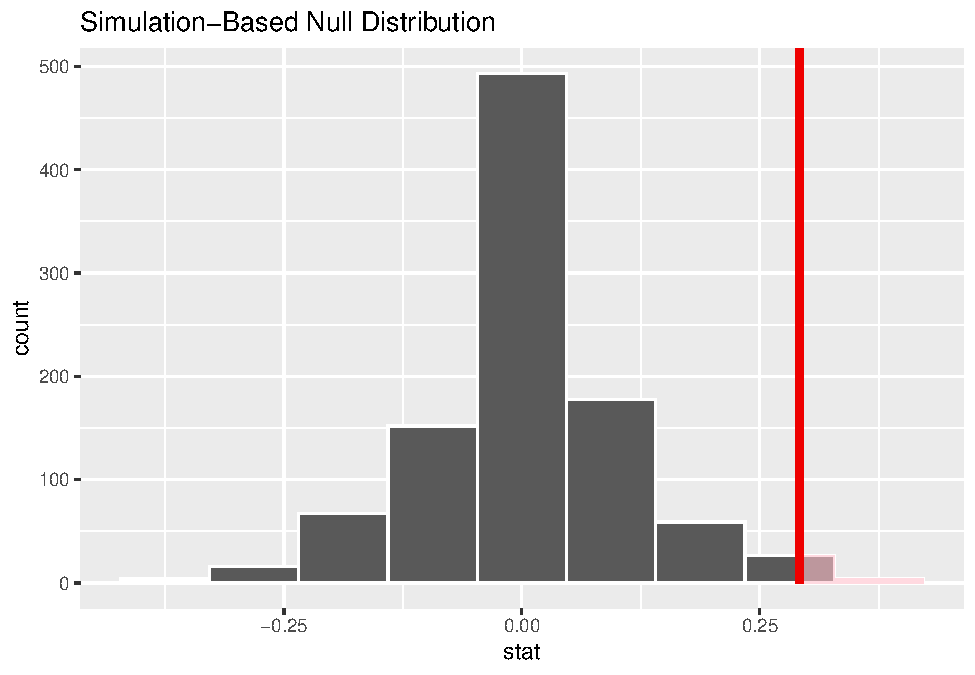
\includegraphics{intro_stats_files/figure-latex/unnamed-chunk-257-1.pdf}

\hypertarget{randomization2-chance}{%
\section{By chance?}\label{randomization2-chance}}

How likely is it that the observed difference (or a difference even more extreme) could have resulted from chance alone? Because \texttt{sims} contains simulated results after permuting, the values in the \texttt{stat} column assume that promotion is independent of sex. In order to assess how plausible our observed difference is under that assumption, we want to find out how many of the simulated values are at least as big, if not bigger, than the observed difference, 0.292.

Look at the randomized differences sorted in decreasing order:

\begin{Shaded}
\begin{Highlighting}[]
\NormalTok{sims }\SpecialCharTok{\%\textgreater{}\%}
    \FunctionTok{arrange}\NormalTok{(}\FunctionTok{desc}\NormalTok{(stat))}
\end{Highlighting}
\end{Shaded}

\begin{verbatim}
## Response: decision (factor)
## Explanatory: sex (factor)
## Null Hypothesis: independence
## # A tibble: 1,000 x 2
##    replicate  stat
##        <int> <dbl>
##  1       133 0.375
##  2       181 0.375
##  3       568 0.375
##  4       619 0.375
##  5        50 0.292
##  6        68 0.292
##  7        77 0.292
##  8        93 0.292
##  9       111 0.292
## 10       119 0.292
## # ... with 990 more rows
\end{verbatim}

Of the 1000 simulations, the most extreme difference of 37.5\% occurred four times, just by chance. That seems like a pretty extreme value when expecting a value of 0\%, but the laws of probability tell us that extreme values will be observed from time to time, even if rarely. Also recall that the observed difference in the actual data was 29.2\%. This specific value came up quite a bit in our simulated data. In fact, the 31st entry of the sorted data above is the last occurrence of the value 0.292. After that, the next higher larger value is 0.208.

So let's return to the original question. How many simulated values are as large---if not larger---than the observed difference? Apparently, 31 out of 1000, which is 0.031. In other words 3\% of the simulated data is as extreme or more extreme than the actual difference in promotion rates between male files and female files in the real data. That's not very large. In other words, a difference like 29.2\% could occur just by chance---like flipping 10 out of 10 heads or something like that. But it doesn't happen very often.

We can automate this calculation using the function \texttt{get\_p\_value} (similar to \texttt{shade\_p\_value} above) even though we don't yet know what ``p value'' means.

\begin{Shaded}
\begin{Highlighting}[]
\NormalTok{sims }\SpecialCharTok{\%\textgreater{}\%}
    \FunctionTok{get\_p\_value}\NormalTok{(}\AttributeTok{obs\_stat =}\NormalTok{ obs\_diff, }\AttributeTok{direction =} \StringTok{"greater"}\NormalTok{)}
\end{Highlighting}
\end{Shaded}

\begin{verbatim}
## # A tibble: 1 x 1
##   p_value
##     <dbl>
## 1   0.031
\end{verbatim}

\textbf{COPY/PASTE WARNING}: If the observed difference were negative, then extreme values of interest would be \emph{less} than, say, -0.292, not greater than 0.292. You must note if the observed difference is positive or negative and then use ``greater'' or ``less'' as appropriate!

Again, 0.031 is a small number. This shows us that if there were truly no association between promotion and sex, then our data is a rare event. (An observed difference this extreme or more extreme would only occur about 3\% of the time by chance.)

Because the probability above is so small, it seems unlikely that our variables are independent. Therefore, it seems more likely that there is an association between promotion and sex. We have evidence of a statistically significant difference between the chance of getting recommended for promotion if the file indicates male versus female.

Because this is an experiment, it's possible that a causal claim could be made. If everything in the application files was identical except the indication of gender, then it stands to reason that gender \emph{explains} why more male files were promoted over female files. But all that depends on the experiment being a well-designed experiment.

\hypertarget{exercise-7-3}{%
\paragraph*{Exercise 7}\label{exercise-7-3}}
\addcontentsline{toc}{paragraph}{Exercise 7}

Although we are not experts in experimental design, what concerns do you have about generalizing the results of this experiment to broad conclusions about sexism in the 1970s?
(To be clear, I'm not saying that sexism wasn't a broad problem in the 1970s. It surely was---and still is. I'm only asking you to opine as to why the results of this one study might not be conclusive in making an overly broad statement.)

Please write up your answer here.

\hypertarget{randomization2-your-turn}{%
\section{Your turn}\label{randomization2-your-turn}}

In this section, you'll explore another famous data set related to the topic of gender discrimination. (Also from the 1970s!)

The following code will download admissions data from the six largest graduate departments at the University of California, Berkeley in 1973. We've seen the \texttt{read\_csv} command before, but we've added some extra stuff in there to make sure all the columns get imported as factor variables (rather than having to convert them ourselves later).

\begin{Shaded}
\begin{Highlighting}[]
\NormalTok{ucb\_admit }\OtherTok{\textless{}{-}} \FunctionTok{read\_csv}\NormalTok{(}\StringTok{"https://vectorposse.github.io/intro\_stats/data/ucb\_admit.csv"}\NormalTok{,}
                      \AttributeTok{col\_types =} \FunctionTok{list}\NormalTok{(}
                          \AttributeTok{Admit =} \FunctionTok{col\_factor}\NormalTok{(),}
                          \AttributeTok{Gender =} \FunctionTok{col\_factor}\NormalTok{(),}
                          \AttributeTok{Dept =} \FunctionTok{col\_factor}\NormalTok{()))}
\end{Highlighting}
\end{Shaded}

\begin{Shaded}
\begin{Highlighting}[]
\NormalTok{ucb\_admit}
\end{Highlighting}
\end{Shaded}

\begin{verbatim}
## # A tibble: 4,526 x 3
##    Admit    Gender Dept 
##    <fct>    <fct>  <fct>
##  1 Admitted Male   A    
##  2 Admitted Male   A    
##  3 Admitted Male   A    
##  4 Admitted Male   A    
##  5 Admitted Male   A    
##  6 Admitted Male   A    
##  7 Admitted Male   A    
##  8 Admitted Male   A    
##  9 Admitted Male   A    
## 10 Admitted Male   A    
## # ... with 4,516 more rows
\end{verbatim}

\begin{Shaded}
\begin{Highlighting}[]
\FunctionTok{glimpse}\NormalTok{(ucb\_admit)}
\end{Highlighting}
\end{Shaded}

\begin{verbatim}
## Rows: 4,526
## Columns: 3
## $ Admit  <fct> Admitted, Admitted, Admitted, Admitted, Admitted, Admitted, Adm~
## $ Gender <fct> Male, Male, Male, Male, Male, Male, Male, Male, Male, Male, Mal~
## $ Dept   <fct> A, A, A, A, A, A, A, A, A, A, A, A, A, A, A, A, A, A, A, A, A, ~
\end{verbatim}

As you go through the exercises below, you should carefully copy and paste commands from earlier in the chapter, making the necessary changes.

\textbf{Remember that R is case sensitive! In the \texttt{sex\_discrimination} data, all the variables and levels started with lowercase letters. In the \texttt{ucb\_admit} data, they all start with uppercase letters, so you'll need to be careful to change that after you copy and paste code examples from above.}

\hypertarget{exercise-8a-2}{%
\paragraph*{Exercise 8(a)}\label{exercise-8a-2}}
\addcontentsline{toc}{paragraph}{Exercise 8(a)}

Is this data observational or experimental? How do you know?

Please write up your answer here.

\hypertarget{exercise-8b-2}{%
\paragraph*{Exercise 8(b)}\label{exercise-8b-2}}
\addcontentsline{toc}{paragraph}{Exercise 8(b)}

Exploratory data analysis: make two contingency tables with \texttt{Admit} as the response variable and \texttt{Gender} as the explanatory variable. One table should have counts and the other table should have percentages. (Both tables should include the marginal distribution at the bottom.)

\begin{Shaded}
\begin{Highlighting}[]
\CommentTok{\# Add code here to make a contingency table with counts.}
\end{Highlighting}
\end{Shaded}

\begin{Shaded}
\begin{Highlighting}[]
\CommentTok{\# Add code here to make a contingency table with percentages.}
\end{Highlighting}
\end{Shaded}

\hypertarget{exercise-8c}{%
\paragraph*{Exercise 8(c)}\label{exercise-8c}}
\addcontentsline{toc}{paragraph}{Exercise 8(c)}

Use \texttt{observe} from the \texttt{infer} package to calculate the observed difference in proportions between males who were admitted and females who were admitted. Do the subtraction in that order: males minus females. Store your output as \texttt{obs\_diff2} so that it doesn't overwrite the variable \texttt{obs\_diff} we created earlier.

\begin{Shaded}
\begin{Highlighting}[]
\CommentTok{\# Add code here to calculate the observed difference.}
\CommentTok{\# Store this as obs\_diff2.}
\end{Highlighting}
\end{Shaded}

\hypertarget{exercise-8d}{%
\paragraph*{Exercise 8(d)}\label{exercise-8d}}
\addcontentsline{toc}{paragraph}{Exercise 8(d)}

Simulate 1000 outcomes under the assumption that admission is independent of gender. Use the \texttt{specify}, \texttt{hypothesize}, \texttt{generate}, and \texttt{calculate} sequence from the \texttt{infer} package as above. Call the simulated data frame \texttt{sims2} so that it doesn't conflict with the earlier \texttt{sims}. Don't touch the \texttt{set.seed} command. That will ensure that all students get the same randomization.

\begin{Shaded}
\begin{Highlighting}[]
\FunctionTok{set.seed}\NormalTok{(}\DecValTok{10101}\NormalTok{)}
\CommentTok{\# Add code here to simulate 1000 outcomes}
\CommentTok{\# under the independence assumption}
\CommentTok{\# and store the simulations in a data frame called sims2.}
\end{Highlighting}
\end{Shaded}

\hypertarget{exercise-8e}{%
\paragraph*{Exercise 8(e)}\label{exercise-8e}}
\addcontentsline{toc}{paragraph}{Exercise 8(e)}

Plot the simulated values in a histogram using the \texttt{visualize} verb from \texttt{infer}. When you first run the code, remove the \texttt{bins\ =\ 9} we had earlier and let \texttt{visualize} choose the number of bins. If you are satisfied with the graph, you don't need to specify a number of bins. If you are not satisfied, you can experiment with the number of bins until you find a number that seems reasonable.

Be sure to include a vertical line at the value of the observed difference using the \texttt{shade\_p\_value} command. Don't forget that the location of that line is \texttt{obs\_diff2} now.

\begin{Shaded}
\begin{Highlighting}[]
\CommentTok{\# Add code here to plot the results.}
\end{Highlighting}
\end{Shaded}

\hypertarget{exercise-8f}{%
\paragraph*{Exercise 8(f)}\label{exercise-8f}}
\addcontentsline{toc}{paragraph}{Exercise 8(f)}

Finally, comment on what you see. Based on the histogram above, is the observed difference in the data rare? In other words, under the assumption that admission and gender are independent, are we likely to see an observed difference as far away from zero as we actually see in the data? So what is your conclusion then? Do you believe there was an association between admission and gender in the UC Berkeley admissions process in 1973?

Please write up your answer here.

\hypertarget{randomization2-simpson}{%
\section{Simpson's paradox}\label{randomization2-simpson}}

The example above from UC Berkeley seems like an open and shut case. Male applicants were clearly admitted at a greater rate than female applicants. While we never expect the application rates to be \emph{exactly} equal---even under the assumption that admission and gender are independent---the randomization exercise showed us that the observed data was \emph{way} outside the range of possible differences that could have occurred just by chance.

But we also know this is observational data. Association is not causation.

\hypertarget{exercise-9-2}{%
\paragraph*{Exercise 9}\label{exercise-9-2}}
\addcontentsline{toc}{paragraph}{Exercise 9}

Note that we didn't say ``correlation is not causation''. The latter is also true, but why does it not apply in this case? (Think about the conditions for correlation.)

Please write up your answer here.

\begin{center}\rule{0.5\linewidth}{0.5pt}\end{center}

Since we don't have data from a carefully controlled experiment, we always have to be worried about lurking variables. Could there be a third variable apart from admission and gender that could be driving the association between them? In other words, the fact that males were admitted at a higher rate than females might be sexism, or it might be spurious.

Since we have access to a third variable, \texttt{Dept}, let's analyze it as well. The \texttt{tabyl} command will happily take a third variable and create a \emph{set} of contingency tables, one for each department.

Here are the tables with counts:

\begin{Shaded}
\begin{Highlighting}[]
\FunctionTok{tabyl}\NormalTok{(ucb\_admit, Admit, Gender, Dept) }\SpecialCharTok{\%\textgreater{}\%}
    \FunctionTok{adorn\_totals}\NormalTok{()}
\end{Highlighting}
\end{Shaded}

\begin{verbatim}
## $A
##     Admit Male Female
##  Admitted  512     89
##  Rejected  313     19
##     Total  825    108
## 
## $B
##     Admit Male Female
##  Admitted  353     17
##  Rejected  207      8
##     Total  560     25
## 
## $C
##     Admit Male Female
##  Admitted  120    202
##  Rejected  205    391
##     Total  325    593
## 
## $D
##     Admit Male Female
##  Admitted  138    131
##  Rejected  279    244
##     Total  417    375
## 
## $E
##     Admit Male Female
##  Admitted   53     94
##  Rejected  138    299
##     Total  191    393
## 
## $F
##     Admit Male Female
##  Admitted   22     24
##  Rejected  351    317
##     Total  373    341
\end{verbatim}

And here are the tables with percentages:

\begin{Shaded}
\begin{Highlighting}[]
\FunctionTok{tabyl}\NormalTok{(ucb\_admit, Admit, Gender, Dept) }\SpecialCharTok{\%\textgreater{}\%}
    \FunctionTok{adorn\_totals}\NormalTok{() }\SpecialCharTok{\%\textgreater{}\%}
    \FunctionTok{adorn\_percentages}\NormalTok{(}\StringTok{"col"}\NormalTok{) }\SpecialCharTok{\%\textgreater{}\%}
    \FunctionTok{adorn\_pct\_formatting}\NormalTok{()}
\end{Highlighting}
\end{Shaded}

\begin{verbatim}
## $A
##     Admit   Male Female
##  Admitted  62.1%  82.4%
##  Rejected  37.9%  17.6%
##     Total 100.0% 100.0%
## 
## $B
##     Admit   Male Female
##  Admitted  63.0%  68.0%
##  Rejected  37.0%  32.0%
##     Total 100.0% 100.0%
## 
## $C
##     Admit   Male Female
##  Admitted  36.9%  34.1%
##  Rejected  63.1%  65.9%
##     Total 100.0% 100.0%
## 
## $D
##     Admit   Male Female
##  Admitted  33.1%  34.9%
##  Rejected  66.9%  65.1%
##     Total 100.0% 100.0%
## 
## $E
##     Admit   Male Female
##  Admitted  27.7%  23.9%
##  Rejected  72.3%  76.1%
##     Total 100.0% 100.0%
## 
## $F
##     Admit   Male Female
##  Admitted   5.9%   7.0%
##  Rejected  94.1%  93.0%
##     Total 100.0% 100.0%
\end{verbatim}

\hypertarget{exercise-10-4}{%
\paragraph*{Exercise 10}\label{exercise-10-4}}
\addcontentsline{toc}{paragraph}{Exercise 10}

Look at the contingency tables with percentages. Examine each department individually. What do you notice about the admit rates (as percentages) between males and females for most of the departments listed? Identify the four departments where female admission rates were higher than male admission rates.

Please write up your answer here.

\begin{center}\rule{0.5\linewidth}{0.5pt}\end{center}

This is completely counterintuitive. How can males be admitted at a higher rate overall, and yet in most departments, females were admitted at a higher rate.

This phenomenon is often called \emph{Simpson's Paradox}. Like almost everything in statistics, this is named after a person (Edward H. Simpson) who got the popular credit for writing about the phenomenon, but not being the person who actually discovered the phenomenon. (There does not appear to be a primeval reference for the first person to have studied it. Similar observations had appeared in various sources more than 50 years before Simpson wrote his paper.)

\hypertarget{exercise-11-4}{%
\paragraph*{Exercise 11}\label{exercise-11-4}}
\addcontentsline{toc}{paragraph}{Exercise 11}

Look at the contingency tables with counts. Focus on the four departments you identified above. What is true of the total number of male and female applicants for those four department (and not for the other two departments)?

Please write up your answer here.

\hypertarget{exercise-12a-1}{%
\paragraph*{Exercise 12(a)}\label{exercise-12a-1}}
\addcontentsline{toc}{paragraph}{Exercise 12(a)}

Now create a contingency table with percentages that uses \texttt{Admit} for the row variable and \texttt{Dept} as the column variable.

\begin{Shaded}
\begin{Highlighting}[]
\CommentTok{\# Add code here to create a contingency table with percentages}
\CommentTok{\# for Dept and Admit}
\end{Highlighting}
\end{Shaded}

\hypertarget{exercise-12b-1}{%
\paragraph*{Exercise 12(b)}\label{exercise-12b-1}}
\addcontentsline{toc}{paragraph}{Exercise 12(b)}

In the contingency table above, what's true about the admission rates for the four departments you identified above (and not true for the other two department)?

Please write up your answer here.

\begin{center}\rule{0.5\linewidth}{0.5pt}\end{center}

Your work in the previous exercises begins to paint a picture that explains what's going on with this ``paradox''. Males applied in greater numbers to departments with high acceptance rates. As a result, more male students overall got in to graduate school. Females applied in greater numbers to departments that were more selective. Overall, then, fewer females got in to graduate school. But on a department-by-department basis, female applicants were usually more likely to get accepted.

None of this suggests that sexism fails to exist. It doesn't even prove that sexism wasn't a factor in some departmental admission procedures. What it does suggest is that when we don't take into account possible lurking variables, we run the risk of oversimplifying issues that are potentially complex.

In our analysis of the UC Berkeley data, we've exhausted all the variables available to us in the data set. There remains the potential for \emph{unmeasured confounders}, or variables that could still act as lurking variables, but we have no idea about them because they aren't in our data. This is an unavoidable peril of working with observational data. If we aren't careful to ``control'' for a reasonable set of possible lurking variables, we must be very careful when trying to make broad conclusions.

\hypertarget{randomization2-conclusion}{%
\section{Conclusion}\label{randomization2-conclusion}}

Here we used randomization to explore the idea of two variables being independent or associated. When we assume they are independent, we can explore the sampling variability of the differences that could occur by pure chance alone. We expect the difference to be zero, but we know that randomness will cause the simulated differences to have a range of values. Is the difference in the observed data far away from zero? In that case, we can say we have evidence that the variables are not independent; in other words, it is more likely that our variables are associated.

\hypertarget{randomization2-prep}{%
\subsection{Preparing and submitting your assignment}\label{randomization2-prep}}

\begin{enumerate}
\def\labelenumi{\arabic{enumi}.}
\tightlist
\item
  From the ``Run'' menu, select ``Restart R and Run All Chunks''.
\item
  Deal with any code errors that crop up. Repeat steps 1---2 until there are no more code errors.
\item
  Spell check your document by clicking the icon with ``ABC'' and a check mark.
\item
  Hit the ``Preview'' button one last time to generate the final draft of the \texttt{.nb.html} file.
\item
  Proofread the HTML file carefully. If there are errors, go back and fix them, then repeat steps 1--5 again.
\end{enumerate}

If you have completed this chapter as part of a statistics course, follow the directions you receive from your professor to submit your assignment.

\hypertarget{hypothesis1}{%
\chapter{Hypothesis testing with randomization, Part 1}\label{hypothesis1}}

2.0

\hypertarget{functions-introduced-in-this-chapter-9}{%
\subsection*{Functions introduced in this chapter}\label{functions-introduced-in-this-chapter-9}}
\addcontentsline{toc}{subsection}{Functions introduced in this chapter}

\texttt{drop\_na}, \texttt{pull}

\hypertarget{hypothesis1-intro}{%
\section{Introduction}\label{hypothesis1-intro}}

Using a sample to deduce something about a population is called ``statistical inference''. In this chapter, we'll learn about one form of statistical inference called ``hypothesis testing''. The focus will be on walking through the example from Part 2 of ``Introduction to randomization'' and recasting it here as a formal hypothesis test.

There are no new R commands here, but there are many new ideas that will require careful reading. You are not expected to be an expert on hypothesis testing after this one chapter. However, within the next few chapters, as we learn more about hypothesis testing and work through many more examples, the hope is that you will begin to assimilate and internalize the logic of inference and the steps of a hypothesis test.

\hypertarget{hypothesis1-install}{%
\subsection{Install new packages}\label{hypothesis1-install}}

There are no new packages used in this chapter.

\hypertarget{hypothesis1-download}{%
\subsection{Download the R notebook file}\label{hypothesis1-download}}

Check the upper-right corner in RStudio to make sure you're in your \texttt{intro\_stats} project. Then click on the following link to download this chapter as an R notebook file (\texttt{.Rmd}).

https://vectorposse.github.io/intro\_stats/chapter\_downloads/10-hypothesis\_testing\_with\_randomization\_1.Rmd

Once the file is downloaded, move it to your project folder in RStudio and open it there.

\hypertarget{hypothesis1-restart}{%
\subsection{Restart R and run all chunks}\label{hypothesis1-restart}}

In RStudio, select ``Restart R and Run All Chunks'' from the ``Run'' menu.

\hypertarget{hypothesis1-load}{%
\section{Load packages}\label{hypothesis1-load}}

We load \texttt{tidyverse} and \texttt{janitor}. We'll continue to explore the \texttt{infer} package for investigating statistical claims. We load the \texttt{openintro} package to access the \texttt{sex\_discrimination} data (the one with the male bank managers promoting male files versus female files).

\begin{Shaded}
\begin{Highlighting}[]
\FunctionTok{library}\NormalTok{(tidyverse)}
\FunctionTok{library}\NormalTok{(janitor)}
\FunctionTok{library}\NormalTok{(infer)}
\FunctionTok{library}\NormalTok{(openintro)}
\end{Highlighting}
\end{Shaded}

\hypertarget{hypothesis1-question}{%
\section{Our research question}\label{hypothesis1-question}}

We return to the sex discrimination experiment from the last chapter. We are interested in finding out if there is an association between the recommendation to promote a candidate for branch manager and the gender listed on the file being evaluated by the male bank manager.

\hypertarget{hypothesis1-hypothesis-testing}{%
\section{Hypothesis testing}\label{hypothesis1-hypothesis-testing}}

The approach we used in Part 2 of ``Introduction to randomization'' was to assume that the two variables \texttt{decision} and \texttt{sex} were independent. From that assumption, we were able to compare the observed difference in promotion percentages between males and females from the actual data to the distribution of random values obtained by randomization. When the observed difference was far enough away from zero, we concluded that the assumption of independence was probably false, giving us evidence that the two variables were associated after all.

This logic is formalized into a sequence of steps known as a \emph{hypothesis test}. In this section, we will introduce a rubric for conducting a full and complete hypothesis test for the sex discrimination example. The file {[}LINK HERE{]} shows the steps for each part of the rubric.

A hypothesis test can be organized into five parts:

\begin{enumerate}
\def\labelenumi{\arabic{enumi}.}
\tightlist
\item
  Exploratory data analysis
\item
  Hypotheses
\item
  Model
\item
  Mechanics
\item
  Conclusion
\end{enumerate}

Below, I'll address each of these steps.

\hypertarget{hypothesis1-eda}{%
\subsection{Exploratory data analysis}\label{hypothesis1-eda}}

Before we can answer questions using data, we need to understand our data.

Most data sets come with some information about the provenance and structure of the data. (Often this is called ``metadata''.) Data provenance is the story of how the data was collected and for what purpose. Together with some information about the types of variables recorded, this is the who, what, when, where, why, and how. Without context, data is just a bunch of letters and numbers. You must understand the nature of the data in order to use the data. Information about the structure of the data is often recorded in a ``code book''.

For data that you collect yourself, you'll already know all about it, although should probably write that stuff down in case other people want to use your data (or in case ``future you'' wants to use the data). For other data sets, you hope that other people have recorded information about how the data was collected and what is described in the data. When working with data sets in R as we do for these chapters, we've already seen that there are help files---sometimes more or less helpful. In some cases, you'll need to go beyond the brief explanations in the help file to investigate the data provenance. And for files we download from other places on the internet, we may have a lot of work to do.

\hypertarget{exercise-1-7}{%
\paragraph*{Exercise 1}\label{exercise-1-7}}
\addcontentsline{toc}{paragraph}{Exercise 1}

What are some ethical issues you might want to consider when looking into the provenance of data? Have a discussion with a classmate and/or do some internet sleuthing to see if you can identify one or two key issues that should be considered before you access or analyze data.

Please write up your answer here.

For exploring the raw data in front of us, we can use commands like \texttt{View} from the Console to see the data in spreadsheet form, although if we're using R Notebooks, we can just type the name of the data frame in a code chunk and run it to print the data in a form we can navigate and explore. There is also \texttt{glimpse} to explore the structure of the data (the variables and how they're coded), as well as other summary functions to get a quick sense of the variables.

Sometimes you have to prepare your data for analysis. A common example is converting categorical variables that should be coded as factor variables, but often are coded as character vectors, or are coded numerically (like ``1'' and ``0'' instead of ``Yes'' and ``No''). Sometimes missing data is coded unusually (like ``999'') and that has to be fixed before trying to calculate statistics. ``Cleaning'' data is often a task that takes more time than analyzing it!

Finally, once the data is in a suitably tidy form, we can use visualizations like tables, graphs, and charts to understand the data better. Often, there are conditions about the shape of our data that have to be met before inference is appropriate, and this step can help diagnose problems that could arise in the inferential procedure. This is a good time to look for outliers, for example.

\hypertarget{hypothesis1-hypotheses}{%
\subsection{Hypotheses}\label{hypothesis1-hypotheses}}

We are trying to ask some question about a population of interest. However, all we have in our data is a sample of that population. The word inference comes from the verb ``infer'': we are trying to infer what might be true of a population just from examining a sample. It's also possible that our question involves comparing two or more populations to each other. In this case, we'll have multiple samples, one from each of our populations. For example, in our sex discrimination example, we are comparing two populations: male bank managers who consider male files for promotion, and male bank managers who consider female files for promotion. Our data gives us two samples who form only a part of the larger populations of interest.

To convince our audience that our analysis is correct, it makes sense to take a skeptical position. If we are trying to prove that there is an association between promotion and sex, we don't just declare it to be so. We start with a ``null hypothesis'', or an expression of the belief that there is no association. A null hypothesis always represents the ``default'' position that a skeptic might take. It codifies the idea that ``there's nothing to see here.''

Our job is to gather evidence to show that there is something interesting going on. The statement of interest to us is called the ``alternative hypothesis''. This is usually the thing we're trying to prove related to our research question.

We can perform \emph{one-sided} tests or \emph{two-sided} tests. A one-sided test is when we have a specific direction in mind for the effect. For example, if we are trying to prove that male files are \emph{more} likely to be promoted than female files, then we would perform a one-sided test. On the other hand, if we only care about proving an association, then male files could be either more likely or less likely to be promoted than female files. (This is contrasted to the null that states that male files are \emph{equally} likely to be promoted as female files.) If it seems weird to run a two-sided test, keep in mind that we want to give our statistical analysis a chance to prove an association regardless of the direction of the association. Wouldn't you be interested to know if it turned out that male files are, in fact, \emph{less} likely to be promoted?

You can't cheat and look at the data first. In a normal research study out there in the real world, you develop hypotheses long before you collect data. So you have to decide to do a one-sided or two-sided test before you have the luxury of seeing your data pointing in one direction or the other.

Running a two-sided test is often a good default option. Again, this is because our analysis will allow us to show interesting effects in any direction.

We typically express hypotheses in two ways. First, we write down full sentences that express in the context of the problem what our null and alternative hypotheses are stating. Then, we express the same ideas as mathematical statements. This translation from words to math is important as it gives us the connection to the quantitative statistical analysis we need to perform. The null hypothesis will always be that some quantity is equal to (=) the null value. The alternative hypothesis depends on whether we are conducting a one-sided test or a two-sided test. A one-sided test is mathematically saying that the quantity of interest is either greater than (\textgreater) or less than (\textless) the null value. A two-sided test always states that the quantity of interest is not equal to (\(\neq\)) the null value. (Notice the math symbol enclosed in dollar signs in the previous sentence. In the HTML file, these symbols will appear correctly. In the R Notebook, you can hover the cursor anywhere between the dollar signs and the math symbol will show up. Alternatively, you can click somewhere between the dollar signs and hit Ctrl-Enter or Cmd-Enter, just like with inline R code.)

The most important thing to know is that the entire hypothesis test up until you reach the conclusion is conducted \textbf{under the assumption that the null hypothesis is true}. In other words, we pretend the whole time that our alternative hypothesis is false, and we carry out our analysis working under that assumption. This may seem odd, but it makes sense when you remember that the goal of inference is to try to convince a skeptic. Others will only believe your claim after you present evidence that suggests that the data is inconsistent with the claims made in the null.

\hypertarget{hypothesis1-model}{%
\subsection{Model}\label{hypothesis1-model}}

A model is an approximation---usually a simplification---of reality. In a hypothesis test, when we say ``model'' we are talking specifically about the ``null model''. In other words, what is true about the population under the assumption of the null? If we sample from the population repeatedly, we find that there is some kind of distribution of values that can occur by pure chance alone. This is called the \emph{sampling distribution model}. We have been learning about how to use randomization to understand the sampling distribution and how much sampling variability to expect, even when the null hypothesis is true.

Building a model is contingent upon certain assumptions being true. We cannot usually demonstrate directly that these assumptions are conclusively met; however, there are often conditions that can be checked with our data that can give us some confidence in saying that the assumptions are probably met. For example, there is no hope that we can infer anything from our sample unless that sample is close to a random sample of the population. There is rarely any direct evidence of having a properly random sample, and often, random samples are too much to ask for. There is almost never such a thing as a truly random sample of the population. Nevertheless, it is up to us to make the case that our sample is as representative of the population as possible. Additionally, we have to know that our sample comprises less than 10\% of the size of the population. The reasons for this are somewhat technical and the 10\% figure is just a rough guideline, but we should think carefully about this whenever we want our inference to be correct.

Those are just two examples. For the randomization tests we are running, those are the only two conditions we need to check. For other hypothesis tests in the future that use different types of models, we will need to check more conditions that correspond to the modeling assumptions we will need to make.

\hypertarget{hypothesis1-mechanics}{%
\subsection{Mechanics}\label{hypothesis1-mechanics}}

This is the nitty-gritty, nuts-and-bolts part of a hypothesis test. Once we have a model that tells us how data should behave under the assumption of the null hypothesis, we need to check how our data actually behaved. The measure of where our data is relative to the null model is called the \emph{test statistic}. For example, if the null hypothesis states that there should be a difference of zero between promotion rates for males and females, then the test statistic would be the actual observed difference in our data between males and females.

Once we have a test statistic, we can plot it in the same graph as the null model. This gives us a visual sense of how rare or unusual our observed data is. The further our test statistic is from the center of the null model, the more evidence we have that our data would be very unusual if the null model were true. And that, in turn, gives us a reason not to believe the null model. When conducting a two-sided test, we will actually graph locations on both side of the null value: the test statistic on one side of the null value and a point the same distance on the other side of the null value. This will acknowledge that we're interested in evidence of an effect in either direction.

Finally, we convert the visual evidence explained in the previous paragraph to a number called a \emph{P-value}. This measures how likely it is to see our observed data---or data even more extreme---under the assumption of the null. A small P-value, then, means that if the null were really true, we wouldn't be very likely at all to see data like ours. That leaves us with little confidence that the null model is really true. (After all, we \emph{did} see the data we gathered!) If the P-value is large---in other words, if the test statistic is closer to the middle of the null distribution---then our data is perfectly consistent with the null hypothesis. That doesn't mean the null is true, but it certainly does not give us evidence against the null.

A one-sided test will give us a P-value that only counts data more extreme than the observed data in the direction that we explicitly hypothesized. For example, if our alternative hypothesis was that male files are more likely to be promoted, then we would only look at the part of the model that showed differences with as many or more male promotions as our data showed. A two-sided P-value, by contrast, will count data that is extreme in either direction. This will include values on both sides of the distribution, which is why it's called a two-sided test. Computationally, it is usually easiest to calculate the one-sided P-value and just double it.\footnote{This is not technically the most mathematically appropriate thing to do, but it's a reasonable approximation in many common situations.}

Remember the statement made earlier that throughout the hypothesis testing process, \textbf{we work under the assumption that the null hypothesis is true}. The P-value is no exception. It tells us \textbf{under the assumption of the null} how likely we are to to see data at least as extreme (if not even more extreme) as the data we actually saw.

\hypertarget{hypothesis1-ht-conclusion}{%
\subsection{Conclusion}\label{hypothesis1-ht-conclusion}}

The P-value we calculate in the Mechanics section allows us to determine what our decision will be relative to the null hypothesis. As explained above, when the P-value is small, that means we had data that would be very unlikely had the null been true. The sensible conclusion is then to ``reject the null hypothesis.'' On the other hand, if the data is consistent with the null hypothesis, then we ``fail to reject the null hypothesis.''

How small does the P-value need to be before we are willing to reject the null hypothesis? That is a decision we have to make based on how much we are willing to risk an incorrect conclusion. A value that is widely used is 0.05; in other words, if \(P < 0.05\) we reject the null, and if \(P > 0.05\), we fail to reject the null. However, for situations where we want to be conservative, we could choose this threshold to be much smaller. If we insist that the P-value be less than 0.01, for example, then we will only reject the null when we have a lot more evidence. The threshold we choose is called the ``significance level'', denoted by the Greek letter alpha: \(\alpha\). The value of \(\alpha\) must be chosen long before we compute our P-value so that we're not tempted to cheat and change the value of \(\alpha\) to suit our P-value (and by doing so, quite literally, move the goalposts).

\textbf{Note that we never accept the null hypothesis.} The hypothesis testing procedure gives us no evidence in favor of the null. All we can say is that the evidence is either strong enough to warrant rejection of the null, or else it isn't, in which case we can conclude nothing. If we can't prove the null false, we are left not knowing much of anything at all.

The phrases ``reject the null'' or ``fail to reject the null'' are very statsy. Your audience may not be statistically trained. Besides, the \emph{real} conclusion you care about concerns the research question of interest you posed at the beginning of this process, and that is built into the alternative hypothesis, not the null. Therefore, we need some statement that addresses the alternative hypothesis in words that a general audience will understand. I recommend the following templates:

\begin{itemize}
\item
  When you reject the null, you can safely say, ``We have sufficient evidence that {[}restate the alternative hypothesis{]}.''
\item
  When you fail to reject the null, you can safely say, ``We have insufficient evidence that {[}restate the alternative hypothesis{]}.''
\end{itemize}

The last part of your conclusion should be an acknowledgement of the uncertainty in this process. Statistics tries to tame randomness, but in the end, randomness is always somewhat unpredictable. It is possible that we came to the wrong conclusion, not because we made mistakes in our computation, but because statistics just can't be right 100\% of the time when randomness is involved. Therefore, we need to explain to our audience that we may have made an error.

A \emph{Type I} error is what happens when the null hypothesis is actually true, but our procedure rejects it anyway. This happens when we get an unrepresentative extreme sample for some reason. For example, perhaps there really is no association between promotion and sex. Even if that were true, we could accidentally survey a group of bank managers who---by pure chance alone---happen to recommend promotion more often for the male files. Our test statistic will be ``accidentally'' far from the null value, and we will mistakenly reject the null. Whenever we reject the null, we are at risk of making a Type I error. Given that we are conclusively stating a statistically significant finding, if that finding is wrong, this is a \emph{false positive}, a term that is synonymous with a Type I error. The significance level \(\alpha\) discussed above is, in fact, the probability of making a Type I error. (If the null is true, we will still reject the null if our P-value happens to be less than \(\alpha\).)

On the other hand, the null may actually be false, and yet, we may not manage to gather enough evidence to disprove it. This can also happen due to an unusual sample---a sample that doesn't conform to the ``truth''. But there are other ways this can happen as well, most commonly when you have a small sample size (which doesn't allow you to prove much of anything at all) or when the effect you're trying to measure exists, but is so small that it is hard to distinguish from no effect at all (which is what the null postulates). In these cases, we are at risk of making a \emph{Type II} error. Anytime we say that we fail to reject the null, we have to worry about the possibility of making a Type II error, also called a \emph{false negative}.

\hypertarget{hypothesis1-example}{%
\section{Example}\label{hypothesis1-example}}

Below, we'll model the process of walking through a complete hypothesis test, showing how we would address each step. Then, you'll have a turn at doing the same thing for a different question. Unless otherwise stated, we will always assume a significance level of \(\alpha = 0.05\). (In other words, we will reject the null if our computed P-value is less than 0.05, and we will fail to reject the null if our P-value is greater than or equal to 0.05.)

Note that there is some mathematical formatting. As mentioned before, this is done by enclosing such math in dollar signs. Don't worry too much about the syntax; just mimic what you see in the example.

\hypertarget{hypothesis1-ex-eda}{%
\section{Exploratory data analysis}\label{hypothesis1-ex-eda}}

\hypertarget{hypothesis1-ex-documentation}{%
\subsection{Use data documentation (help files, code books, Google, etc.) to determine as much as possible about the data provenance and structure.}\label{hypothesis1-ex-documentation}}

You can look at the help file by typing \texttt{?sex\_discrimination} at the Console. (However, do not put that command here in a code chunk. The R Notebook has no way of displaying a help file when it's processed.) You can also type that into the Help tab in the lower-right panel in RStudio.

The help file doesn't say too much, but there is a ``Source'' at the bottom. We can do an internet search for ``Rosen Jerdee Influence of sex role stereotypes on personnel decisions''. As many academics articles on the internet are, this one is pay-walled, so we can't read it for free. If you go to school or work for an institution with a library, though, you may be able to access articles through your library services. Talk to a librarian if you'd like to access research articles. As long as you have the citation details, librarians can often track down articles, and many are already accessible through library databases.

In this case, we can read the abstract for free. This tells us that the data we have is only one part of a larger set of experiments done.

This is also the place to comment on any ethical concerns you may have. For example, how was the data collected? Did the researchers follow ethical guidelines in the treatment of their subjects, like obtaining consent? Without accessing the full article, it's hard to know in this case. But do your best in each data analysis task you have to try to find out as much as possible about the data.

In this section, we'll also print the data set and use \texttt{glimpse} to summarize the variables.

\begin{Shaded}
\begin{Highlighting}[]
\NormalTok{sex\_discrimination}
\end{Highlighting}
\end{Shaded}

\begin{verbatim}
## # A tibble: 48 x 2
##    sex   decision
##    <fct> <fct>   
##  1 male  promoted
##  2 male  promoted
##  3 male  promoted
##  4 male  promoted
##  5 male  promoted
##  6 male  promoted
##  7 male  promoted
##  8 male  promoted
##  9 male  promoted
## 10 male  promoted
## # ... with 38 more rows
\end{verbatim}

\begin{Shaded}
\begin{Highlighting}[]
\FunctionTok{glimpse}\NormalTok{(sex\_discrimination)}
\end{Highlighting}
\end{Shaded}

\begin{verbatim}
## Rows: 48
## Columns: 2
## $ sex      <fct> male, male, male, male, male, male, male, male, male, male, m~
## $ decision <fct> promoted, promoted, promoted, promoted, promoted, promoted, p~
\end{verbatim}

\hypertarget{hypothesis1-ex-prepare}{%
\subsection{Prepare the data for analysis.}\label{hypothesis1-ex-prepare}}

In this section, we do any tasks required to clean the data. This will often involve using \texttt{mutate}, either to convert other variable types to factors, or compute additional variables using existing columns. It may involve using \texttt{filter} to analyze only one part of the data we care about.

If there is missing data, this is the place to identify it and decide if you need to address it before starting your analysis. It's always important to check for missing data. It's not always necessary to address it now as many of the R functions we use will ignore rows with missing data.

The easiest way to detect missing data is to try deleting rows that are missing some data with \texttt{drop\_na} and see if the number of rows changes:

\begin{Shaded}
\begin{Highlighting}[]
\NormalTok{sex\_discrimination }\SpecialCharTok{\%\textgreater{}\%}
  \FunctionTok{drop\_na}\NormalTok{()}
\end{Highlighting}
\end{Shaded}

\begin{verbatim}
## # A tibble: 48 x 2
##    sex   decision
##    <fct> <fct>   
##  1 male  promoted
##  2 male  promoted
##  3 male  promoted
##  4 male  promoted
##  5 male  promoted
##  6 male  promoted
##  7 male  promoted
##  8 male  promoted
##  9 male  promoted
## 10 male  promoted
## # ... with 38 more rows
\end{verbatim}

Since the result still has 48 rows, there are no missing values.

The \texttt{sex\_discimination} data is already squeaky clean, so we don't need to do anything here.

\hypertarget{hypothesis1-ex-plots}{%
\subsection{Make tables or plots to explore the data visually.}\label{hypothesis1-ex-plots}}

As we have two categorical variables, a contingency table is a good way of visualizing the distribution of both variables together. (Don't forget to include the marginal distribution and create two tables: one with counts and one with percentages!)

\begin{Shaded}
\begin{Highlighting}[]
\FunctionTok{tabyl}\NormalTok{(sex\_discrimination, decision, sex) }\SpecialCharTok{\%\textgreater{}\%}
  \FunctionTok{adorn\_totals}\NormalTok{()}
\end{Highlighting}
\end{Shaded}

\begin{verbatim}
##      decision male female
##      promoted   21     14
##  not promoted    3     10
##         Total   24     24
\end{verbatim}

\begin{Shaded}
\begin{Highlighting}[]
\FunctionTok{tabyl}\NormalTok{(sex\_discrimination, decision, sex) }\SpecialCharTok{\%\textgreater{}\%}
  \FunctionTok{adorn\_totals}\NormalTok{() }\SpecialCharTok{\%\textgreater{}\%}
  \FunctionTok{adorn\_percentages}\NormalTok{(}\StringTok{"col"}\NormalTok{) }\SpecialCharTok{\%\textgreater{}\%}
  \FunctionTok{adorn\_pct\_formatting}\NormalTok{()}
\end{Highlighting}
\end{Shaded}

\begin{verbatim}
##      decision   male female
##      promoted  87.5%  58.3%
##  not promoted  12.5%  41.7%
##         Total 100.0% 100.0%
\end{verbatim}

\hypertarget{hypothesis1-ex-hypotheses}{%
\section{Hypotheses}\label{hypothesis1-ex-hypotheses}}

\hypertarget{hypothesis1-ex-sample-pop}{%
\subsection{Identify the sample (or samples) and a reasonable population (or populations) of interest.}\label{hypothesis1-ex-sample-pop}}

There are technically two samples of interest here. All the data comes from a group of 48 bank managers recruited for the study, but one group of interest are bank managers who are evaluating male files, and the other group of interest are bank managers who are evaluating female files.

One of the contingency tables above shows the sample sizes for each group in the marginal distribution along the bottom of the table (i.e., the column sums). There are 24 mangers with male files and 24 managers with female files.

The populations of interest are probably all bank managers evaluating male candidates and all bank managers evaluating female candidates, probably only in in the U.S. (where the two researchers were based) and only during the 1970s.

\hypertarget{hypothesis1-ex-express-words}{%
\subsection{Express the null and alternative hypotheses as contextually meaningful full sentences.}\label{hypothesis1-ex-express-words}}

(Note: The null hypothesis is indicated by the symbol \(H_{0}\), often pronounced ``H naught'' or ``H sub zero.'' The alternative hypothesis is indicated by \(H_{A}\), pronounced ``H sub A.'')

\(H_{0}:\) There is no association between decision and sex in hiring branch managers for banks in the 1970s.

\(H_{A}:\) There is an association between decision and sex in hiring branch managers for banks in the 1970s.

\hypertarget{hypothesis1-ex-express-math}{%
\subsection{Express the null and alternative hypotheses in symbols (when possible).}\label{hypothesis1-ex-express-math}}

\(H_{0}: p_{promoted, male} - p_{promoted, female} = 0\)

\(H_{A}: p_{promoted, male} - p_{promoted, female} \neq 0\)

Note: First, pay attention to the ``success'' condition (in this case, ``promoted''). We could choose to measure either those promoted or those not promoted. The difference will be positive for one and negative for the other, so it really doesn't matter which one we choose. Just make a choice and be consistent. Also pay close attention here to the order of the subtraction. Again, while it doesn't matter conceptually, we need to make sure that the code we include later agrees with this order.

\hypertarget{hypothesis1-ex-model}{%
\section{Model}\label{hypothesis1-ex-model}}

\hypertarget{hypothesis1-ex-sampling-dist-model}{%
\subsection{Identify the sampling distribution model.}\label{hypothesis1-ex-sampling-dist-model}}

We will randomize to simulate the sampling distribution.

\hypertarget{hypothesis1-ex-conditions}{%
\subsection{Check the relevant conditions to ensure that model assumptions are met.}\label{hypothesis1-ex-conditions}}

\begin{itemize}
\tightlist
\item
  Random (for both groups)

  \begin{itemize}
  \tightlist
  \item
    We have no evidence that these are random samples of bank managers. We hope that they are representative. If the populations of interest are all bank managers in the U.S. evaluating either male candidates or female candidates, then we have some doubts as to how representative these samples are. It is likely that the bank managers were recruited from limited geographic areas based on the location of the researchers, and we know that geography could easily be a confounder for sex discrimination (because some areas of the country might be more prone to it than others). Despite our misgivings, we will proceed on with the analysis, but we will temper our expectations for grand, sweeping conclusions.
  \end{itemize}
\item
  10\% (for both groups)

  \begin{itemize}
  \tightlist
  \item
    Regardless of the intended populations, 24 bank managers evaluating male files and 24 bank managers evaluating female files are surely less than 10\% of all bank managers under consideration.
  \end{itemize}
\end{itemize}

\hypertarget{hypothesis1-ex-mechanics}{%
\section{Mechanics}\label{hypothesis1-ex-mechanics}}

\hypertarget{hypothesis1-ex-compute-test-stat}{%
\subsection{Compute the test statistic.}\label{hypothesis1-ex-compute-test-stat}}

We let \texttt{infer} do the work here:

\begin{Shaded}
\begin{Highlighting}[]
\NormalTok{obs\_diff }\OtherTok{\textless{}{-}}\NormalTok{ sex\_discrimination }\SpecialCharTok{\%\textgreater{}\%}
    \FunctionTok{observe}\NormalTok{(decision }\SpecialCharTok{\textasciitilde{}}\NormalTok{ sex, }\AttributeTok{success =} \StringTok{"promoted"}\NormalTok{,}
            \AttributeTok{stat =} \StringTok{"diff in props"}\NormalTok{, }\AttributeTok{order =} \FunctionTok{c}\NormalTok{(}\StringTok{"male"}\NormalTok{, }\StringTok{"female"}\NormalTok{))}
\NormalTok{obs\_diff}
\end{Highlighting}
\end{Shaded}

\begin{verbatim}
## Response: decision (factor)
## Explanatory: sex (factor)
## # A tibble: 1 x 1
##    stat
##   <dbl>
## 1 0.292
\end{verbatim}

Note: \texttt{obs\_diff} is a tibble, albeit a small one, having only one column and one row. That tibble is what we need to feed into the visualization later. However, for reporting the value by itself, we have to pull it out of the tibble. We will do this below using the \texttt{pull} function. See the inline code in the next subsection.

\hypertarget{hypothesis1-ex-report-test-stat}{%
\subsection{Report the test statistic in context (when possible).}\label{hypothesis1-ex-report-test-stat}}

The observed difference in the proportion of promotion recommendations for male files versus female files is 0.2916667 (subtracting males minus females). Or, another way to say this: there is a 29.1666667\% difference in the promotion rates between male files and female files.

\hypertarget{hypothesis1-ex-plot-null}{%
\subsection{Plot the null distribution.}\label{hypothesis1-ex-plot-null}}

Note: In this section, we will use the series of verbs from \texttt{infer} to generate all the information we need about the hypothesis test. We call that output \texttt{decision\_sex\_test} here, but you'll want to change it to another name for a different test. The recommended pattern is \texttt{response\_predictor\_test}.

Don't forget to set the seed. We are using randomization to permute the values of the predictor variable in order to break any association that might exist in the data. This will allow us to explore the sampling distribution created under the assumption of the null hypothesis.

When you get to the \texttt{visualize} step, leave the number of bins out. (Just type \texttt{visualize()} with empty parentheses.) If you determine that the default binning is not optimal, you can add back \texttt{bins} and experiment with the number. We know from the previous chapter that 9 bins is good here.

\begin{Shaded}
\begin{Highlighting}[]
\FunctionTok{set.seed}\NormalTok{(}\DecValTok{9999}\NormalTok{)}
\NormalTok{decision\_sex\_test }\OtherTok{\textless{}{-}}\NormalTok{ sex\_discrimination }\SpecialCharTok{\%\textgreater{}\%}
    \FunctionTok{specify}\NormalTok{(decision }\SpecialCharTok{\textasciitilde{}}\NormalTok{ sex, }\AttributeTok{success =} \StringTok{"promoted"}\NormalTok{) }\SpecialCharTok{\%\textgreater{}\%}
    \FunctionTok{hypothesize}\NormalTok{(}\AttributeTok{null =} \StringTok{"independence"}\NormalTok{) }\SpecialCharTok{\%\textgreater{}\%}
    \FunctionTok{generate}\NormalTok{(}\AttributeTok{reps =} \DecValTok{1000}\NormalTok{, }\AttributeTok{type =} \StringTok{"permute"}\NormalTok{) }\SpecialCharTok{\%\textgreater{}\%}
    \FunctionTok{calculate}\NormalTok{(}\AttributeTok{stat =} \StringTok{"diff in props"}\NormalTok{, }\AttributeTok{order =} \FunctionTok{c}\NormalTok{(}\StringTok{"male"}\NormalTok{, }\StringTok{"female"}\NormalTok{))}
\NormalTok{decision\_sex\_test}
\end{Highlighting}
\end{Shaded}

\begin{verbatim}
## Response: decision (factor)
## Explanatory: sex (factor)
## Null Hypothesis: independence
## # A tibble: 1,000 x 2
##    replicate    stat
##        <int>   <dbl>
##  1         1 -0.0417
##  2         2  0.208 
##  3         3  0.0417
##  4         4 -0.125 
##  5         5 -0.0417
##  6         6 -0.208 
##  7         7 -0.208 
##  8         8  0.0417
##  9         9 -0.292 
## 10        10  0.125 
## # ... with 990 more rows
\end{verbatim}

\begin{Shaded}
\begin{Highlighting}[]
\NormalTok{decision\_sex\_test }\SpecialCharTok{\%\textgreater{}\%}
    \FunctionTok{visualize}\NormalTok{(}\AttributeTok{bins =} \DecValTok{9}\NormalTok{) }\SpecialCharTok{+}
    \FunctionTok{shade\_p\_value}\NormalTok{(}\AttributeTok{obs\_stat =}\NormalTok{ obs\_diff, }\AttributeTok{direction =} \StringTok{"two{-}sided"}\NormalTok{)}
\end{Highlighting}
\end{Shaded}

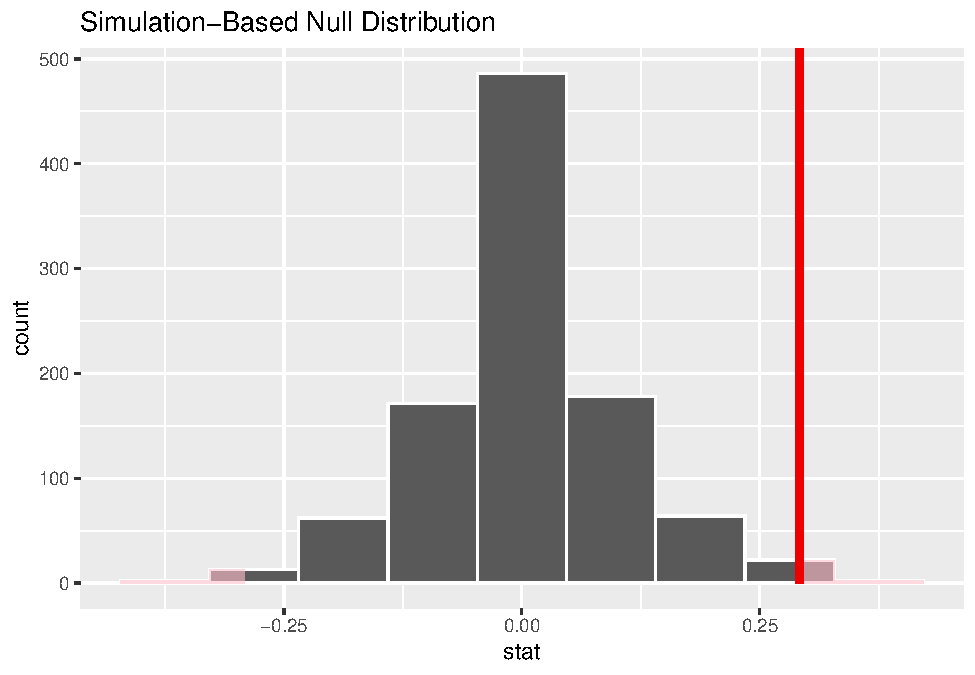
\includegraphics{intro_stats_files/figure-latex/unnamed-chunk-279-1.pdf}

(You'll note that there is light gray shading in \emph{both} tails above. This is because we are conducting a two-sided test, which means that we're interested in values that are more extreme than our observed difference in \emph{both} directions.)

\hypertarget{hypothesis1-ex-calculate-p}{%
\subsection{Calculate the P-value.}\label{hypothesis1-ex-calculate-p}}

\begin{Shaded}
\begin{Highlighting}[]
\NormalTok{P }\OtherTok{\textless{}{-}}\NormalTok{ decision\_sex\_test }\SpecialCharTok{\%\textgreater{}\%}
  \FunctionTok{get\_p\_value}\NormalTok{(}\AttributeTok{obs\_stat =}\NormalTok{ obs\_diff, }\AttributeTok{direction =} \StringTok{"two{-}sided"}\NormalTok{)}
\NormalTok{P}
\end{Highlighting}
\end{Shaded}

\begin{verbatim}
## # A tibble: 1 x 1
##   p_value
##     <dbl>
## 1   0.048
\end{verbatim}

Note: as with the test statistic above, the P-value appears above in a 1x1 tibble. That's fine for this step, but in the inline code below, we will need to use \texttt{pull} again to extract the value.

\hypertarget{hypothesis1-ex-interpret-p}{%
\subsection{Interpret the P-value as a probability given the null.}\label{hypothesis1-ex-interpret-p}}

The P-value is 0.048. If there were no association between decision and sex, there would be a 4.8\% chance of seeing data at least as extreme as we saw.

Some important things here:

\begin{enumerate}
\def\labelenumi{\arabic{enumi}.}
\item
  We include an interpretation for our P-value. Remember that the P-value is the probability---\textbf{under the assumption of the null hypothesis}---of seeing results as extreme or even more extreme than the data we saw.
\item
  The P-value is less than 0.05 (just barely). Remember that as we talk about the conclusion in the next section of the rubric.
\end{enumerate}

\hypertarget{hypothesis1-ex-ht-conclusion}{%
\section{Conclusion}\label{hypothesis1-ex-ht-conclusion}}

\hypertarget{hypothesis1-ex-stat-conclusion}{%
\subsection{State the statistical conclusion.}\label{hypothesis1-ex-stat-conclusion}}

We reject the null hypothesis.

\hypertarget{hypothesis1-ex-context-conclusion}{%
\subsection{State (but do not overstate) a contextually meaningful conclusion.}\label{hypothesis1-ex-context-conclusion}}

There is sufficient evidence to suggest that there is an an association between decision and sex in hiring branch managers for banks in the 1970s.

Note: the easiest thing to do here is just restate the alternative hypothesis. If we reject the null, then we have \emph{sufficient} evidence for the alternative hypothesis. If we fail to reject the null, we have \emph{insufficient} evidence for the alternative hypothesis. Either way, though, this contextually meaningful conclusion is all about the alternative hypothesis.

\hypertarget{hypothesis1-ex-reservations}{%
\subsection{Express reservations or uncertainty about the generalizability of the conclusion.}\label{hypothesis1-ex-reservations}}

We have some reservations about how generalizable this conclusion is due to the fact that we are lacking information about how representative our samples of bank managers were. We also point out that this experiment was conducted in the 1970s, so its conclusions are not valid for today.

Note: This would also be the place to point out any possible sources of bias or confounding that might be present, especially for observational studies.

\hypertarget{hypothesis1-ex-errors}{%
\subsection{Identify the possibility of either a Type I or Type II error and state what making such an error means in the context of the hypotheses.}\label{hypothesis1-ex-errors}}

As we rejected the null, we run the risk of committing a Type I error. It is possible that there is no association between decision and sex, but we've come across a sample in which male files were somehow more likely to be recommended for promotion.

\begin{center}\rule{0.5\linewidth}{0.5pt}\end{center}

After writing up your conclusions and acknowledging the possibility of a Type I or Type II error, the hypothesis test is complete. (At least for now. In the future, we will add one more step of computing a confidence interval.)

\hypertarget{hypothesis1-one-sided-two-sided}{%
\section{More on one-sided and two-sided tests}\label{hypothesis1-one-sided-two-sided}}

I want to emphasize again the difference between conducting a one-sided versus a two-sided test. You may recall that in ``Introduction to simulation, Part 2'', we calculated this:

\begin{Shaded}
\begin{Highlighting}[]
\FunctionTok{set.seed}\NormalTok{(}\DecValTok{9999}\NormalTok{)}
\NormalTok{sex\_discrimination }\SpecialCharTok{\%\textgreater{}\%}
    \FunctionTok{specify}\NormalTok{(decision }\SpecialCharTok{\textasciitilde{}}\NormalTok{ sex, }\AttributeTok{success =} \StringTok{"promoted"}\NormalTok{) }\SpecialCharTok{\%\textgreater{}\%}
    \FunctionTok{hypothesize}\NormalTok{(}\AttributeTok{null =} \StringTok{"independence"}\NormalTok{) }\SpecialCharTok{\%\textgreater{}\%}
    \FunctionTok{generate}\NormalTok{(}\AttributeTok{reps =} \DecValTok{1000}\NormalTok{, }\AttributeTok{type =} \StringTok{"permute"}\NormalTok{) }\SpecialCharTok{\%\textgreater{}\%}
    \FunctionTok{calculate}\NormalTok{(}\AttributeTok{stat =} \StringTok{"diff in props"}\NormalTok{, }\AttributeTok{order =} \FunctionTok{c}\NormalTok{(}\StringTok{"male"}\NormalTok{, }\StringTok{"female"}\NormalTok{)) }\SpecialCharTok{\%\textgreater{}\%}
    \FunctionTok{get\_p\_value}\NormalTok{(}\AttributeTok{obs\_stat =}\NormalTok{ obs\_diff, }\AttributeTok{direction =} \StringTok{"greater"}\NormalTok{)}
\end{Highlighting}
\end{Shaded}

\begin{verbatim}
## # A tibble: 1 x 1
##   p_value
##     <dbl>
## 1   0.024
\end{verbatim}

The justification was that, back then, we already suspected that male files were more likely to be promoted, and it appears that our evidence (the test statistic, or our observed difference) was pretty far in that direction. (Actually, we may get a slightly different number each time. Remember that we are randomizing. Therefore, we won't expect to get the exact same numbers each time.)

By way of contrast, in this chapter we computed the two-sided P-value:

\begin{Shaded}
\begin{Highlighting}[]
\FunctionTok{set.seed}\NormalTok{(}\DecValTok{9999}\NormalTok{)}
\NormalTok{sex\_discrimination }\SpecialCharTok{\%\textgreater{}\%}
    \FunctionTok{specify}\NormalTok{(decision }\SpecialCharTok{\textasciitilde{}}\NormalTok{ sex, }\AttributeTok{success =} \StringTok{"promoted"}\NormalTok{) }\SpecialCharTok{\%\textgreater{}\%}
    \FunctionTok{hypothesize}\NormalTok{(}\AttributeTok{null =} \StringTok{"independence"}\NormalTok{) }\SpecialCharTok{\%\textgreater{}\%}
    \FunctionTok{generate}\NormalTok{(}\AttributeTok{reps =} \DecValTok{1000}\NormalTok{, }\AttributeTok{type =} \StringTok{"permute"}\NormalTok{) }\SpecialCharTok{\%\textgreater{}\%}
    \FunctionTok{calculate}\NormalTok{(}\AttributeTok{stat =} \StringTok{"diff in props"}\NormalTok{, }\AttributeTok{order =} \FunctionTok{c}\NormalTok{(}\StringTok{"male"}\NormalTok{, }\StringTok{"female"}\NormalTok{)) }\SpecialCharTok{\%\textgreater{}\%}
    \FunctionTok{get\_p\_value}\NormalTok{(}\AttributeTok{obs\_stat =}\NormalTok{ obs\_diff, }\AttributeTok{direction =} \StringTok{"two{-}sided"}\NormalTok{)}
\end{Highlighting}
\end{Shaded}

\begin{verbatim}
## # A tibble: 1 x 1
##   p_value
##     <dbl>
## 1   0.048
\end{verbatim}

The only change to the code is the word ``two-sided'' (versus ``greater'') in the last line.

Our P-value in this chapter is twice as large as it could have been if we had run a one-sided test.

Doubling the P-value might mean that it no longer falls under the significance threshold \(\alpha = 0.05\) (although in this case, we still came in under 0.05). This raises an obvious question: why use two-sided tests at all? If the P-values are higher, that makes it less likely that we will reject the null, which means we won't be able to prove our alternative hypothesis. Isn't that a bad thing?

As a matter of fact, there are many researchers in the world who do think it's a bad thing, and routinely do things like use one-sided tests to give them a better chance of getting small P-values. But this is not ethical. The point of research is to do good science, not prove your pet theories correct. There are many incentives in the world for a researcher to prove their theories correct (money, awards, career advancement, fame and recognition, legacy, etc.), but these should be secondary to the ultimate purpose of advancing knowledge. Sadly, many researchers out there have these priorities reversed. I do not claim that researchers set out to cheat; I suspect that the vast majority of researchers act in good faith. Nevertheless, the rewards associated with ``successful'' research cause cognitive biases that are hard to overcome. And ``success'' is often very narrowly defined as research that produces small P-values.

A better approach is to be conservative. For example, a two-sided test is not only more conservative because it produces higher P-values, but also because it answers a more general question. That is, it is scientifically interesting when an association goes in either direction (e.g.~more male promotions, but also possibly more female promotions). This is why we recommended above using two-sided tests by default, and only using a one-sided test when there is a very strong research hypothesis that justifies it.

\hypertarget{hypothesis1-fail-to-reject}{%
\section{A reminder about failing to reject the null}\label{hypothesis1-fail-to-reject}}

It's also important to remember that when we fail to reject the null hypothesis, we are not saying that the null hypothesis is true. Neither are we saying it's false. Failure to reject the null is really a failure to conclude anything at all. But rather than looking at it as a failure, a more productive viewpoint is to see it as an opportunity for more research, possibly with larger sample sizes.

Even when we do reject the null, it is important not to see that as the end of the conversation. Too many times, a researcher publishes a ``statistically significant'' finding in a peer-reviewed journal, and then that result is taken as ``Truth''. We should, instead, view statistical inference as incremental knowledge that works slowly to refine our state of scientific knowledge, as opposed to a collection of ``facts'' and ``non-facts''.

\hypertarget{hypothesis1-your-turn}{%
\section{Your turn}\label{hypothesis1-your-turn}}

Now it's your turn to run a complete hypothesis test. Determine if males were admitted to the top six UC Berkeley grad programs at a higher rate than females. For purposes of this exercise, we will not take into account the \texttt{Dept} variable as we did in the last chapter when we discussed Simpson's Paradox. But as that is a potential source of confounding, be sure to mention it in the part of the rubric where you discuss reservations about your conclusion.

As always, use a significance level of \(\alpha = 0.05\).

Here is the data import:

\begin{Shaded}
\begin{Highlighting}[]
\NormalTok{ucb\_admit }\OtherTok{\textless{}{-}} \FunctionTok{read\_csv}\NormalTok{(}\StringTok{"https://vectorposse.github.io/intro\_stats/data/ucb\_admit.csv"}\NormalTok{,}
                      \AttributeTok{col\_types =} \FunctionTok{list}\NormalTok{(}
                          \AttributeTok{Admit =} \FunctionTok{col\_factor}\NormalTok{(),}
                          \AttributeTok{Gender =} \FunctionTok{col\_factor}\NormalTok{(),}
                          \AttributeTok{Dept =} \FunctionTok{col\_factor}\NormalTok{()))}
\end{Highlighting}
\end{Shaded}

I have copied the template below. You need to fill in each step. Some of the steps will be the same or similar to steps in the example above. It is perfectly okay to copy and paste R code, making the necessary changes. It is \textbf{not} okay to copy and paste text. You need to put everything into your own words. Also, don't copy and paste the parts that are labeled as ``Notes''. That is information to help you understand each step, but it's not part of the statistical analysis itself.

The template below is exactly the same as in the file {[}LINK HERE{]} up to the part about confidence intervals which we haven't learned yet.

\hypertarget{exploratory-data-analysis}{%
\paragraph*{Exploratory data analysis}\label{exploratory-data-analysis}}
\addcontentsline{toc}{paragraph}{Exploratory data analysis}

\hypertarget{use-data-documentation-help-files-code-books-google-etc.-to-determine-as-much-as-possible-about-the-data-provenance-and-structure.}{%
\subparagraph*{Use data documentation (help files, code books, Google, etc.) to determine as much as possible about the data provenance and structure.}\label{use-data-documentation-help-files-code-books-google-etc.-to-determine-as-much-as-possible-about-the-data-provenance-and-structure.}}
\addcontentsline{toc}{subparagraph}{Use data documentation (help files, code books, Google, etc.) to determine as much as possible about the data provenance and structure.}

Please write up your answer here

\begin{Shaded}
\begin{Highlighting}[]
\CommentTok{\# Add code here to print the data}
\end{Highlighting}
\end{Shaded}

\begin{Shaded}
\begin{Highlighting}[]
\CommentTok{\# Add code here to glimpse the variables}
\end{Highlighting}
\end{Shaded}

\hypertarget{prepare-the-data-for-analysis.-not-always-necessary.}{%
\subparagraph*{Prepare the data for analysis. {[}Not always necessary.{]}}\label{prepare-the-data-for-analysis.-not-always-necessary.}}
\addcontentsline{toc}{subparagraph}{Prepare the data for analysis. {[}Not always necessary.{]}}

\begin{Shaded}
\begin{Highlighting}[]
\CommentTok{\# Add code here to prepare the data for analysis.}
\end{Highlighting}
\end{Shaded}

\hypertarget{make-tables-or-plots-to-explore-the-data-visually.}{%
\subparagraph*{Make tables or plots to explore the data visually.}\label{make-tables-or-plots-to-explore-the-data-visually.}}
\addcontentsline{toc}{subparagraph}{Make tables or plots to explore the data visually.}

\begin{Shaded}
\begin{Highlighting}[]
\CommentTok{\# Add code here to make tables or plots.}
\end{Highlighting}
\end{Shaded}

\hypertarget{hypotheses}{%
\paragraph*{Hypotheses}\label{hypotheses}}
\addcontentsline{toc}{paragraph}{Hypotheses}

\hypertarget{identify-the-sample-or-samples-and-a-reasonable-population-or-populations-of-interest.}{%
\subparagraph*{Identify the sample (or samples) and a reasonable population (or populations) of interest.}\label{identify-the-sample-or-samples-and-a-reasonable-population-or-populations-of-interest.}}
\addcontentsline{toc}{subparagraph}{Identify the sample (or samples) and a reasonable population (or populations) of interest.}

Please write up your answer here.

\hypertarget{express-the-null-and-alternative-hypotheses-as-contextually-meaningful-full-sentences.}{%
\subparagraph*{Express the null and alternative hypotheses as contextually meaningful full sentences.}\label{express-the-null-and-alternative-hypotheses-as-contextually-meaningful-full-sentences.}}
\addcontentsline{toc}{subparagraph}{Express the null and alternative hypotheses as contextually meaningful full sentences.}

\(H_{0}:\) Null hypothesis goes here.

\(H_{A}:\) Alternative hypothesis goes here.

\hypertarget{express-the-null-and-alternative-hypotheses-in-symbols-when-possible.}{%
\subparagraph*{Express the null and alternative hypotheses in symbols (when possible).}\label{express-the-null-and-alternative-hypotheses-in-symbols-when-possible.}}
\addcontentsline{toc}{subparagraph}{Express the null and alternative hypotheses in symbols (when possible).}

\(H_{0}: math\)

\(H_{A}: math\)

\hypertarget{model}{%
\paragraph*{Model}\label{model}}
\addcontentsline{toc}{paragraph}{Model}

\hypertarget{identify-the-sampling-distribution-model.}{%
\subparagraph*{Identify the sampling distribution model.}\label{identify-the-sampling-distribution-model.}}
\addcontentsline{toc}{subparagraph}{Identify the sampling distribution model.}

Please write up your answer here.

\hypertarget{check-the-relevant-conditions-to-ensure-that-model-assumptions-are-met.}{%
\subparagraph*{Check the relevant conditions to ensure that model assumptions are met.}\label{check-the-relevant-conditions-to-ensure-that-model-assumptions-are-met.}}
\addcontentsline{toc}{subparagraph}{Check the relevant conditions to ensure that model assumptions are met.}

Please write up your answer here. (Some conditions may require R code as well.)

\hypertarget{mechanics}{%
\paragraph*{Mechanics}\label{mechanics}}
\addcontentsline{toc}{paragraph}{Mechanics}

\hypertarget{compute-the-test-statistic.}{%
\subparagraph*{Compute the test statistic.}\label{compute-the-test-statistic.}}
\addcontentsline{toc}{subparagraph}{Compute the test statistic.}

\begin{Shaded}
\begin{Highlighting}[]
\CommentTok{\# Add code here to compute the test statistic.}
\end{Highlighting}
\end{Shaded}

\hypertarget{report-the-test-statistic-in-context-when-possible.}{%
\subparagraph*{Report the test statistic in context (when possible).}\label{report-the-test-statistic-in-context-when-possible.}}
\addcontentsline{toc}{subparagraph}{Report the test statistic in context (when possible).}

Please write up your answer here.

\hypertarget{plot-the-null-distribution.}{%
\subparagraph*{Plot the null distribution.}\label{plot-the-null-distribution.}}
\addcontentsline{toc}{subparagraph}{Plot the null distribution.}

\begin{Shaded}
\begin{Highlighting}[]
\FunctionTok{set.seed}\NormalTok{(}\DecValTok{9999}\NormalTok{)}
\CommentTok{\# Add code here to simulate the null distribution.}
\CommentTok{\# Run 1000 reps like in the earlier example.}
\end{Highlighting}
\end{Shaded}

\begin{Shaded}
\begin{Highlighting}[]
\CommentTok{\# Add code here to plot the null distribution.}
\end{Highlighting}
\end{Shaded}

\hypertarget{calculate-the-p-value.}{%
\subparagraph*{Calculate the P-value.}\label{calculate-the-p-value.}}
\addcontentsline{toc}{subparagraph}{Calculate the P-value.}

\begin{Shaded}
\begin{Highlighting}[]
\CommentTok{\# Add code here to calculate the P{-}value.}
\end{Highlighting}
\end{Shaded}

\hypertarget{interpret-the-p-value-as-a-probability-given-the-null.}{%
\subparagraph*{Interpret the P-value as a probability given the null.}\label{interpret-the-p-value-as-a-probability-given-the-null.}}
\addcontentsline{toc}{subparagraph}{Interpret the P-value as a probability given the null.}

Please write up your answer here.

\hypertarget{conclusion}{%
\paragraph*{Conclusion}\label{conclusion}}
\addcontentsline{toc}{paragraph}{Conclusion}

\hypertarget{state-the-statistical-conclusion.}{%
\subparagraph*{State the statistical conclusion.}\label{state-the-statistical-conclusion.}}
\addcontentsline{toc}{subparagraph}{State the statistical conclusion.}

Please write up your answer here.

\hypertarget{state-but-do-not-overstate-a-contextually-meaningful-conclusion.}{%
\subparagraph*{State (but do not overstate) a contextually meaningful conclusion.}\label{state-but-do-not-overstate-a-contextually-meaningful-conclusion.}}
\addcontentsline{toc}{subparagraph}{State (but do not overstate) a contextually meaningful conclusion.}

Please write up your answer here.

\hypertarget{express-reservations-or-uncertainty-about-the-generalizability-of-the-conclusion.}{%
\subparagraph*{Express reservations or uncertainty about the generalizability of the conclusion.}\label{express-reservations-or-uncertainty-about-the-generalizability-of-the-conclusion.}}
\addcontentsline{toc}{subparagraph}{Express reservations or uncertainty about the generalizability of the conclusion.}

Please write up your answer here.

\hypertarget{identify-the-possibility-of-either-a-type-i-or-type-ii-error-and-state-what-making-such-an-error-means-in-the-context-of-the-hypotheses.}{%
\subparagraph*{Identify the possibility of either a Type I or Type II error and state what making such an error means in the context of the hypotheses.}\label{identify-the-possibility-of-either-a-type-i-or-type-ii-error-and-state-what-making-such-an-error-means-in-the-context-of-the-hypotheses.}}
\addcontentsline{toc}{subparagraph}{Identify the possibility of either a Type I or Type II error and state what making such an error means in the context of the hypotheses.}

Please write up your answer here.

\hypertarget{hypothesis1-conclusion}{%
\section{Conclusion}\label{hypothesis1-conclusion}}

A hypothesis test is a formal set of steps---a procedure, if you will---for implementing the logic of inference. We take a skeptical position and assume a null hypothesis in contrast to the question of interest, the alternative hypothesis. We build a model under the assumption of the null hypothesis to see if our data is consistent with the null (in which case we fail to reject the null) or unusual/rare relative to the null (in which case we reject the null). We always work under the assumption of the null so that we can convince a skeptical audience using evidence. We also take care to acknowledge that statistical procedures can be wrong, and not to put too much credence in the results of any single set of data or single hypothesis test.

\hypertarget{hypothesis1-prep}{%
\subsection{Preparing and submitting your assignment}\label{hypothesis1-prep}}

\begin{enumerate}
\def\labelenumi{\arabic{enumi}.}
\tightlist
\item
  From the ``Run'' menu, select ``Restart R and Run All Chunks''.
\item
  Deal with any code errors that crop up. Repeat steps 1---2 until there are no more code errors.
\item
  Spell check your document by clicking the icon with ``ABC'' and a check mark.
\item
  Hit the ``Preview'' button one last time to generate the final draft of the \texttt{.nb.html} file.
\item
  Proofread the HTML file carefully. If there are errors, go back and fix them, then repeat steps 1--5 again.
\end{enumerate}

If you have completed this chapter as part of a statistics course, follow the directions you receive from your professor to submit your assignment.

  \bibliography{book.bib,packages.bib}

\end{document}
